%\documentclass[a4paper,12pt, draft]{article}

%%% Работа с русским языком
\usepackage{cmap}					% поиск в PDF
\usepackage{mathtext} 				% русские буквы в формулах
\usepackage[T2A]{fontenc}			% кодировка
\usepackage[utf8]{inputenc}			% кодировка исходного текста
\usepackage[english,russian]{babel}	% локализация и переносы
\usepackage{indentfirst}            % красная строка в первом абзаце
\frenchspacing                      % равные пробелы между словами и предложениями
% 
%%% Дополнительная работа с математикой
\usepackage{amsmath,amsfonts,amssymb,amsthm,mathtools} % пакеты AMS
\usepackage{icomma}                                    % "Умная" запятая
% \usepackage{unicode-math} % русский в математике
\usepackage{gensymb} % градус



%%% Свои символы и команды
\usepackage{centernot} % центрированное зачеркивание символа
\usepackage{stmaryrd}  % некоторые спецсимволы
\usepackage{dsfont}
\usepackage{amsthm}

\renewcommand{\epsilon}{\ensuremath{\varepsilon}}
\renewcommand{\phi}{\ensuremath{\varphi}}
\renewcommand{\kappa}{\ensuremath{\varkappa}}
\renewcommand{\le}{\ensuremath{\leqslant}}
\renewcommand{\leq}{\ensuremath{\leqslant}}
\renewcommand{\ge}{\ensuremath{\geqslant}}
\renewcommand{\geq}{\ensuremath{\geqslant}}
\renewcommand{\emptyset}{\ensuremath{\varnothing}}
% \renewcommand{\c}{\cdot}

\DeclareMathOperator{\sgn}{sgn}
\DeclareMathOperator{\ord}{ord}
\DeclareMathOperator{\lcm}{\text{НОК}}
\DeclareMathOperator{\gcdru}{\text{НОД}}
\DeclareMathOperator{\ke}{Ker}
\DeclareMathOperator{\im}{Im}
\DeclareMathOperator{\re}{Re}
\DeclareMathOperator{\orb}{Orb}
\DeclareMathOperator{\stab}{Stab}
\DeclareMathOperator{\charf}{char}
\DeclareMathOperator{\eva}{Eva}


\newcommand{\NN}{\mathbb{N}}
\newcommand{\ZZ}{\mathbb{Z}}
\newcommand{\QQ}{\mathbb{Q}}
\newcommand{\RR}{\mathbb{R}}
\newcommand{\Cm}{\mathbb{C}}
\newcommand{\FF}{\mathbb{F}}
\newcommand{\id}{\mathrm{id}}


\newcommand{\comp}{\circ}
\newcommand{\raone}{\mapsto}
\newcommand{\Ra}{\Rightarrow}
\newcommand{\ra}{\rightarrow}
\newcommand{\hra}{\hookrightarrow}
\newcommand{\La}{\Leftarrow}
\newcommand{\la}{\leftarrow}
\newcommand{\Lra}{\Leftrightarrow}
\newcommand{\lra}{\leftrightarrow}
\renewcommand{\subset}{\subseteq}
\newcommand{\sub}{\subset}
\newcommand{\sconstr}{\;\vert\;}
\newcommand{\thus}{\implies}
\newcommand{\cd}{\cdot}

% \newcommand{\myeq{\stackrel{\mathclap{\normalfont\mbox{def}}}{=}}}
\newcommand{\defeq}{\vcentcolon= }
\newcommand{\defev}{\stackrel{\Delta}{\Longleftrightarrow}}
% \newcommand{\deriv}[3][1]{%
% 	\ifthenelse{#1>1}{%
% 		\frac{\delta^{#1} {#2}}{\delta {#3}^{#1}}
% 	}{%
% 		\frac{\delta {#2}}{\delta {#3}}
% 	}%
% }
\newcommand{\deriv}[3]{\frac{\delta^{#1} {#2}}{\delta {#3}^{#1}}}

\renewcommand{\labelitemi}{$\triangleright$}

% \equalto --- делает вертикальное равно
\newcommand{\verteq}{\rotatebox{90}{$\,=$}}
\newcommand{\equalto}[2]{\underset{\scriptstyle\overset{\mkern4mu\verteq}{#2}}{#1}}


% \let\bs\backslash
% \let\lra\Leftrightarrow
% \let\ra\Rightarrow
% \let\la\Leftarrow
% \let\emb\hookrightarrow

%%% Перенос знаков в формулах (по Львовскому)
\newcommand{\hm}[1]{#1\nobreak\discretionary{}{\hbox{$\mathsurround=0pt #1$}}{}}

%%% Работа с картинками
\usepackage{graphicx}    % Для вставки рисунков
\setlength\fboxsep{3pt}  % Отступ рамки \fbox{} от рисунка
\setlength\fboxrule{1pt} % Толщина линий рамки \fbox{}
\usepackage{wrapfig}     % Обтекание рисунков текстом

%%% Работа с таблицами
\usepackage{array,tabularx,tabulary,booktabs} % Дополнительная работа с таблицами
\usepackage{longtable}                        % Длинные таблицы
\usepackage{multirow}                         % Слияние строк в таблице

%%% Теоремы
\theoremstyle{plain}
\newtheorem*{theorem}{Теорема}
\newtheorem*{lemma}{Лемма}
\newtheorem*{proposition}{Утверждение}
\newtheorem*{exercise}{Упражнение}
\newtheorem*{problem}{Задача}

\theoremstyle{definition}
\newtheorem*{definition}{Определение}
\newtheorem*{corollary}{Следствие}
\newtheorem*{note}{Замечание}
\newtheorem*{reminder}{Напоминание}
\newtheorem*{example}{Пример}

\theoremstyle{remark}
\newtheorem*{solution}{Решение}

%%% Оформление страницы
\usepackage{extsizes}     % Возможность сделать 14-й шрифт
\usepackage{geometry}     % Простой способ задавать поля
\usepackage{setspace}     % Интерлиньяж
\usepackage{enumitem}     % Настройка окружений itemize и enumerate
\setlist{leftmargin=20pt} % Отступы в itemize и enumerate

\geometry{top=25mm}    % Поля сверху страницы
\geometry{bottom=30mm} % Поля снизу страницы
\geometry{left=20mm}   % Поля слева страницы
\geometry{right=20mm}  % Поля справа страницы

\setlength\parindent{15pt}        % Устанавливает длину красной строки 15pt
\linespread{1}                  % Коэффициент межстрочного интервала
%\setlength{\parskip}{0.5em}      % Вертикальный интервал между абзацами
\setcounter{secnumdepth}{0}      % Отключение нумерации разделов
%\setcounter{section}{-1}         % Нумерация секций с нуля
\usepackage{multicol}			  % Для текста в нескольких колонках
\usepackage{soulutf8}             % Модификаторы начертания
\mathtoolsset{showonlyrefs=true} % показывать номера формул только у тех, у которых есть ссылки по eqref
%%% Содержаниие
\usepackage{tocloft}
\tocloftpagestyle{main}
%\setlength{\cftsecnumwidth}{2.3em}
%\renewcommand{\cftsecdotsep}{1}
%\renewcommand{\cftsecpresnum}{\hfill}
%\renewcommand{\cftsecaftersnum}{\quad}

%%% Шаблонная информация для титульного листа
\newcommand{\CourseName}{Основы Высшей Алгебры и Теории Кодирования}
\newcommand{\FullCourseNameFirstPart}{\so{ОСНОВЫ ВЫСШЕЙ АЛГЕБРЫ И ТЕОРИИ КОДИРОВАНИЯ}}
\newcommand{\SemesterNumber}{II}
\newcommand{\LecturerInitials}{Вялый Михаил Николаевич}
\newcommand{\CourseDate}{Весна 2023}
\newcommand{\AuthorInitials}{Юдин Иван}
\newcommand{\VKLink}{https://vk.com/prk_gufik}
\newcommand{\GithubLink}{https://github.com/daniild71r/lectures_tex_club}

%%% Колонтитулы
\usepackage{titleps}
\newpagestyle{main}{
	\setheadrule{0.4pt}
	\sethead{\CourseName}{}{\hyperlink{intro}{\;Назад к содержанию}}
	\setfootrule{0.4pt}                       
	\setfoot{ФПМИ МФТИ, \CourseDate}{}{\thepage} 
}
\pagestyle{main}  

%%% Нумерация уравнений
\makeatletter
\def\eqref{\@ifstar\@eqref\@@eqref}
\def\@eqref#1{\textup{\tagform@{\ref*{#1}}}}
\def\@@eqref#1{\textup{\tagform@{\ref{#1}}}}
\makeatother                      % \eqref* без гиперссылки
\numberwithin{equation}{section}  % Нумерация вида (номер_секции).(номер_уравнения)
\mathtoolsset{showonlyrefs= true} % Номера только у формул с \eqref{} в тексте.

%%% Гиперссылки
\usepackage{hyperref}
\usepackage[usenames,dvipsnames,svgnames,table,rgb]{xcolor}
\hypersetup{
	unicode=true,            % русские буквы в раздела PDF
	colorlinks=true,       	 % Цветные ссылки вместо ссылок в рамках
	linkcolor=black!15!blue, % Внутренние ссылки
	citecolor=green,         % Ссылки на библиографию
	filecolor=magenta,       % Ссылки на файлы
	urlcolor=NavyBlue,       % Ссылки на URL
}

%%% Графика
\usepackage{tikz}        % Графический пакет tikz
\usepackage{tikz-cd}     % Коммутативные диаграммы
\usepackage{tkz-euclide} % Геометрия
\usepackage{stackengine} % Многострочные тексты в картинках
\usetikzlibrary{angles, babel, quotes}

%\includeonly{lectures/lect05,lectures/lect06}  % Скомпилировать только часть лекций

\begin{document}
    \begin{titlepage}
	\clearpage\thispagestyle{empty}
	\centering
	
	\textbf{Московский физико-технический институт \\ Физтех-школа прикладной математики и информатики}
	\vspace{33ex}
	
	{\textbf{\FullCourseNameFirstPart}}
	
	\SemesterNumber\ СЕМЕСТР  
	\vspace{1ex}
	
	Лектор: \textit{\LecturerInitials}
	
	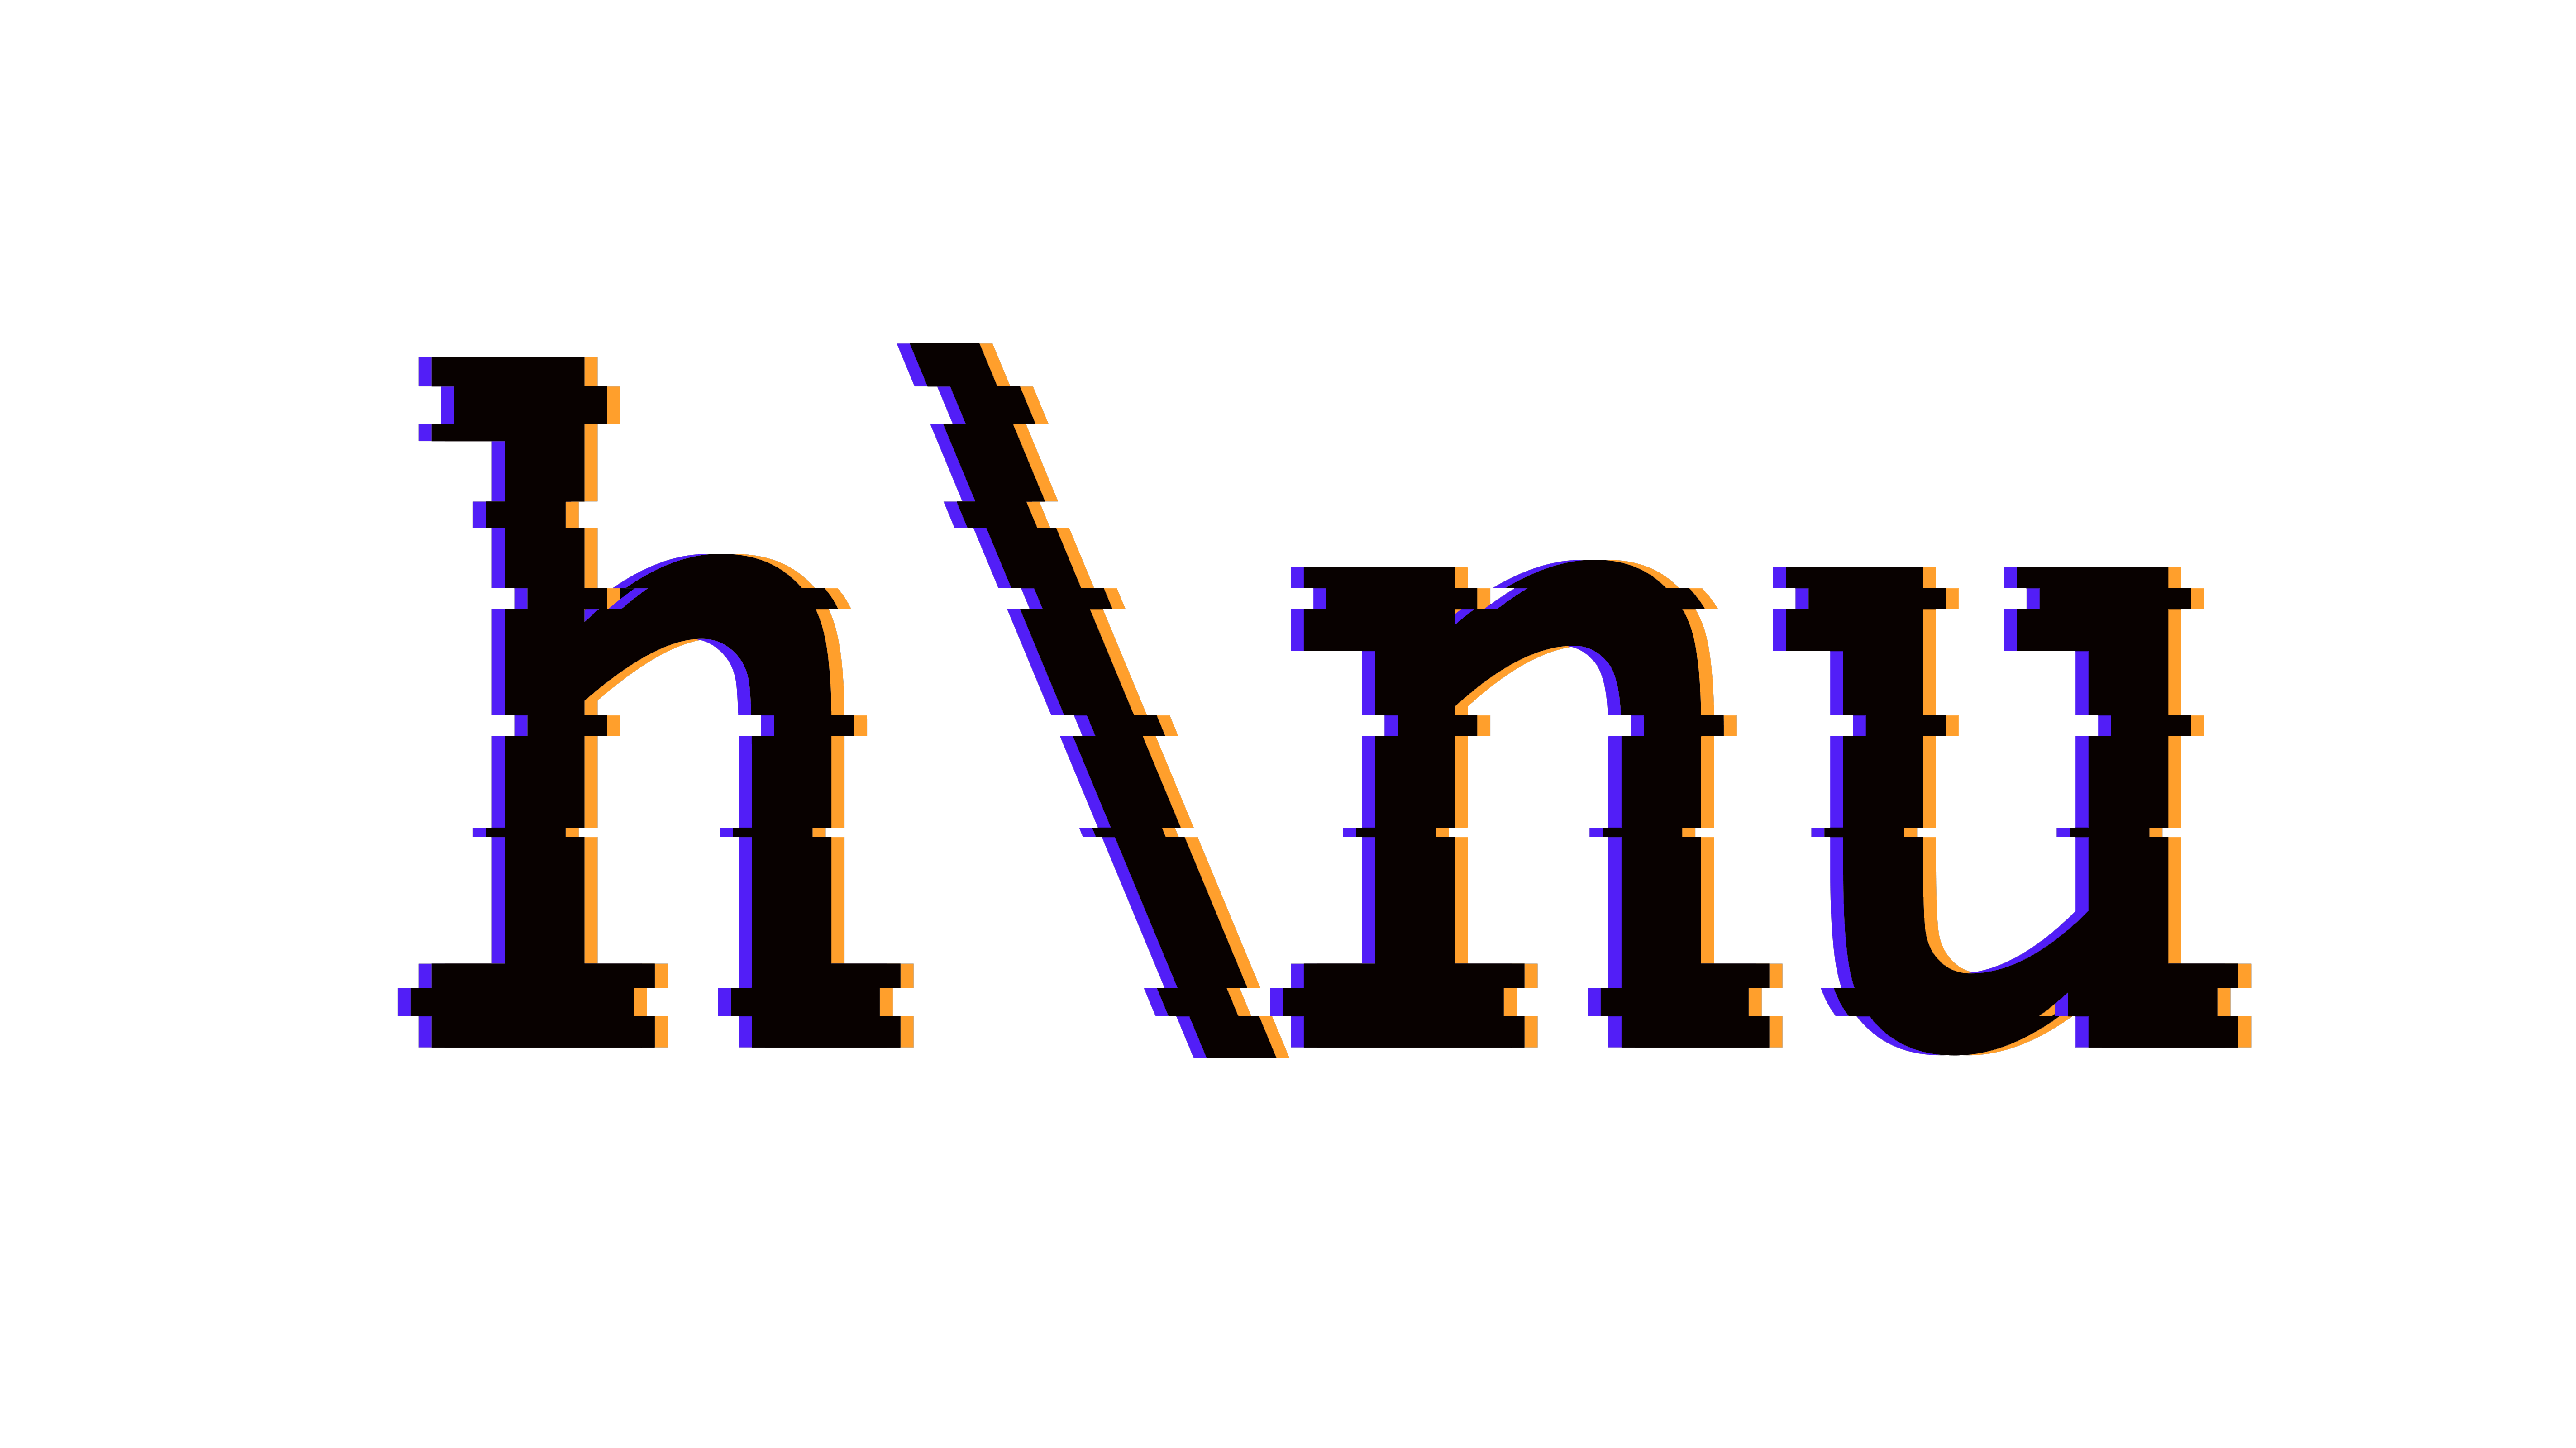
\includegraphics[width=0.4\textwidth]{images/logo_ltc.png}

	\begin{flushright}
		\noindent
		Автор:  \href{\VKLink}{\textit{\AuthorInitials}}, \href{\VKLinksecond}{\textit{\AuthorInitialssecond}}

		\href{\GithubLink}{\textit{Проект на Github}}
	\end{flushright}
	
	\vfill
	\CourseDate
	\pagebreak
\end{titlepage}
    \newpage
    \hypertarget{intro}{}
    \tableofcontents
    
    \linespread{1}
    \selectfont
    
    \newpage

    % 2023 reTeXed Lectures:
    \section{Ряды Фурье}

\begin{note}
	Мы рассматриваем только измеримые функции, если не оговорено обратного.
\end{note}

\subsection{Коэффициенты Фурье}

\begin{proposition}
	Множество функций, суммируемых со своим квадратом на промежутке $I \subset \R$ (то есть для функции $f$ рассматривается $f^2(x) = f(x) \cdot f(x)$), образует линейное пространство.
\end{proposition}

\begin{proof}
	Нужно показать замкнутость относительно сложения. Заметим, что из суммируемости функций $f_1, f_2$ со своим квадратом следует суммируемость $f_1 \cdot f_2$. Действительно, произведение измеримо по известному свойству, а также есть неравенство:
	\[
		\forall x \in I\ \ |f_1(x) \cdot f_2(x)| \le \frac{1}{2}(f_1^2(x) + f_2^2(x))
	\]
	То есть суммируемость произведения установлена по признаку суммируемости. Остаётся расписать квадрат от суммы функций и увидеть, что правая часть тоже суммируема:
	\[
		(f_1 + f_2)^2 = f_1^2 + 2f_1f_2 + f_2^2
	\]
\end{proof}

\begin{note}
	На полученном линейном пространстве можно ввести <<скалярное произведение>> следующим образом:
	\[
		\tbr{f, g} := \int_I f(x)g(x)d\mu(x)
	\]
	Проблема в том, что для него не выполнено всего одно из свойств:
	\[
		\forall x \in I\ \tbr{f, f} = 0 \centernot\Ra f = 0
	\]
\end{note}

\begin{note}
	Нарушение свойства у <<скалярного произведения>> можно исправить, если перейти к линейному пространству классов эквивалентности функций. По чему будет эквивалентность? Достаточно вспомнить факт:
	\[
		\tbr{f, f} = \int_I f^2(x)d\mu(x) = 0 \Lra f = 0 \text{ почти всюду на } I
	\]
	Стало быть, определим эквивалентность на функциях следующим образом:
	\[
		f \sim g \Longleftrightarrow \tbr{f - g, f - g} = 0
	\]
	Доказательство того, что этим задано отношение эквивалентности, оставляется читателю в качестве домашнего задания (Спойлер: мы это уже делали для пространств $L_1$, ибо введённая эквивалентность по сути требует совпадение функций почти всюду на $I$).
\end{note}

\begin{definition}
	Линейное пространство классов эквивалентных функций, измеримых и суммируемых со своим квадратом на $I$, обозначается как $L_2(I)$.
\end{definition}

\begin{anote}
	Для линейного пространства всех функций, измеримых и суммируемых со своим квадратом на $I$, иногда используют обозначение $\cL_2(I)$. Мы будем просто писать $f \in L_2(I)$ --- представитель класса из $L_2(I)$, если не оговорено обратного.
\end{anote}

\begin{corollary}
	$L_2(I)$ является евклидовым пространством с тем скалярным произведением, которое мы определили. Благодаря этому выполняется неравенство Коши-Буняковского-Шварца:
	\[
		\forall f, g \in L_2(I)\ \ |\tbr{f, g}|^2 \le \tbr{f, f} \cdot \tbr{g, g}
	\]
	Или же в раскрытой форме:
	\[
		\md{\int_I f(x)g(x)d\mu(x)} \le \ps{\int_I f^2(x)d\mu(x)}^{1/2} \cdot \ps{\int_I g^2(x)d\mu(x)}^{1/2}
	\]
	Оно же ещё называется \textit{интегральным неравенством Коши-Буняковского-Шварца}.
\end{corollary}

\begin{note}
	Заметим, что $f \in L_2(I) \lra |f| \in L_2(I)$, а поэтому имеет место и такое неравенство:
	\[
		\int_I |f(x)g(x)|d\mu(x) \le \ps{\int_I f^2(x)d\mu(x)}^{1/2} \cdot \ps{\int_I g^2(x)d\mu(x)}^{1/2}
	\]
\end{note}

\begin{anote}
	Вообще говоря, при введении скалярного произведения на $L_2(I)$ мы руководствуемся представителями классов. Стало быть, надо доказывать корректность, но мы это опускаем (и это, к тому же, достаточно просто).
\end{anote}

\begin{proposition}
	$L_2(I)$ является линейно-нормированным пространством (ЛНП) с нормой следующего вида:
	\[
		\|f\|_{L_2} = \sqrt{\tbr{f, f}} = \sqrt{\int_I f^2(x)d\mu(x)}
	\]
\end{proposition}

\begin{proof}
	Доказывалось то ли в первом, то ли во втором семестре. Нужно проверить аксиомы нормы.
\end{proof}

\begin{definition}
	Система функций $\{e_i(x)\}_{i = 1}^\infty \subseteq L_2(I)$ называется \textit{ортогональной}, если выполнено условие:
	\[
		\forall i \neq j\ \ \tbr{e_i, e_j} = 0
	\]
\end{definition}

\begin{definition}
	Если $\{e_i\}_{i = 1}^\infty$ --- ортогональная система ненулевых функций, то \textit{коэффициенты Фурье для функции $f \in L_2(I)$ по этой системе} определяются так:
	\[
			\forall k \in \N\ \ \alpha_k = \frac{\tbr{f, e_k}}{\tbr{e_k, e_k}}
	\]
	А ряд $\sum_{k = 1}^\infty \alpha_k e_k$ называется \textit{рядом Фурье функции $f$ по системе $e_i$}.
\end{definition}

\begin{example}
	Рассмотрим несколько примеров ортогональных систем:
	\begin{enumerate}
		\item \textit{Многочленами Лежандра} называется ряд многочленов следующего вида:
		\begin{align*}
			&{L_0(x) = 1}
			\\
			&{L_n(x) = \frac{1}{2^n n!} \cdot \frac{d^n}{dx^n} (x^2 - 1)^n,\ n > 0}
		\end{align*}
		Утверждается, что они образуют ортогональную систему в $L_2[-1; 1]$. Попробуем вычислить скалярное произведение $\tbr{L_n, L_k}$ для любых $n > k \ge 0$. Для начала докажем, что
		\[
			\forall j \le n\ \ \frac{d^j}{dx^j}(x^2 - 1)^n = (x - 1)^{n - j} p_j(x)
		\]
		где $p_j(x)$ --- многочлен степени $n$. Сделать это можно индукцией по $j$:
		\begin{itemize}
			\item База $j = 0$: тривиально
			
			\item Переход $j > 0$: распишем производную
			\begin{multline*}
				\frac{d^{j + 1}}{dx^{j + 1}}(x^2 - 1)^n = \frac{d}{dx}\ps{(x - 1)^{n - j}p_j(x)} = (n - j)(x - 1)^{n - j - 1}p_j(x) + (x - 1)^{n - j}p'_j(x) =
				\\
				(x - 1)^{n - j - 1}p_{j + 1}(x)
			\end{multline*}
			Из этих равенств уже можно выяснить явный вид многочлена $p_{j + 1}(x)$, который соответствует утверждению индукции.
		\end{itemize}
		Более того, аналогичное утверждение верно и в таком виде:
		\[
			\forall j \le n\ \ \frac{d^j}{dx^j}(x^2 - 1)^n = (x + 1)^{n - j}q_j(x)
		\]
		где $q_j(x)$ тоже степени $n$. Доказательство абсолютно аналогичное, а общим следствием для этих двух фактов будет такое равенство:
		\[
			\forall j \le n\ \ \frac{d^j}{dx^j}(x^2 - 1)^n\Big|_{x = \pm 1} = 0
		\]
		Теперь мы готовы к расписыванию скалярного произведения. Если вынести коэффициенты многочленов, то остаётся разобраться с таким интегралом:
		\begin{multline*}
			\int_{-1}^1 \frac{d^n}{dx^n}(x^2 - 1)^n \cdot \frac{d^k}{dx^k}(x^2 - 1)^kdx =
			\\
			\underbrace{\frac{d^{n - 1}}{dx^{n - 1}}(x^2 - 1)^n \cdot \frac{d^k}{dx^k}(x^2 - 1)^k\Big|_{-1}^1}_0 - \int_{-1}^1 \frac{d^{n - 1}}{dx^{n - 1}}(x^2 - 1)^n \cdot \frac{d^{k + 1}}{dx^{k + 1}}(x^2 - 1)^kdx =
			\\
			\ldots = (-1)^n \int_{-1}^1 (x^2 - 1)^n \frac{d^{k + n}}{dx^{k + n}}(x^2 - 1)^kdx
		\end{multline*}
		Коль скоро $k + n > 2k$, то производная порядка $k + n$ от многочлена степени $2k$ не может не занулится, то есть
		\[
			\int_{-1}^1 \frac{d^n}{dx^n}(x^2 - 1)^n \cdot \frac{d^k}{dx^k}(x^2 - 1)^kdx = (-1)^n \int_{-1}^1 (x^2 - 1)^n \frac{d^{k + n}}{dx^{k + n}}(x^2 - 1)^kdx = 0
		\]
		
		\item \textit{Тригонометрической системой} называется система функций $\{1 / 2, \cos nx,\ \sin nx \such n \in \N\}$, рассматриваемая в $L_2[a; a + 2\pi]$. Так как интеграл по периоду периодической функции не зависит от смещения начальной точки, то рассмотрим $a = -\pi$ и докажем в этом случае ортогональность:
		\begin{itemize}
			\item \(\forall n \in \N \int_{-\pi}^\pi \cos(nx)dx = 0\) --- тривиально
			
			\item \(\forall n \in \N \int_{-\pi}^\pi \sin(nx)dx = 0\) --- тривиально
			
			\item Рассмотрим $\tbr{\cos(nx), \cos(mx)},\ m \neq n$:
			\begin{multline*}
				\int_{-\pi}^\pi \cos(nx)\cos(mx)dx = \frac{1}{2} \int_{-\pi}^\pi (\cos((m + n)x) + \cos((m - n)x))dx =
				\\
				\frac{1}{2(m + n)}\sin((m + n)x)\Big|_{-\pi}^\pi + \frac{1}{2(m - n)}\sin((m - n)x)\Big|_{-\pi}^\pi = 0
			\end{multline*}
			
			\item Случай $\tbr{\sin(nx), \sin(mx)},\ m \neq n$ разбирается аналогично
			
			\item Случай $\tbr{\sin(nx), \cos(mx)},\ m, n \in \N$ разбирается аналогично
		\end{itemize}
		Посчитаем \textit{тригонометрические коэффициенты Фурье} для произвольной функции $f$:
		\begin{itemize}
			\item \[
				a_0 = \frac{\tbr{f, 1 / 2}}{\tbr{1 / 2, 1 / 2}} = \frac{1}{\pi} \int_{-\pi}^\pi f(x)d\mu(x)
			\]
			
			\item \[
				\forall n \in \N\ \ a_n = \frac{\tbr{f, \cos(nx)}}{\tbr{\cos(nx), \cos(nx)}} = \frac{\int_{-\pi}^\pi f(x)\cos(nx)d\mu(x)}{\int_{-\pi}^\pi \cos^2(nx)d\mu(x)} = \frac{1}{\pi} \int_{-\pi}^\pi f(x)\cos(nx)d\mu(x)
			\]
			
			\item \[
				\forall n \in \N\ \ b_n = \frac{\tbr{f, \sin(nx)}}{\tbr{\sin(nx), \sin(nx)}} = \frac{1}{\pi} \int_{-\pi}^\pi f(x)\sin(nx)d\mu(x)
			\]
		\end{itemize}
	\end{enumerate}
\end{example}

\begin{definition}
	Пусть $f \in L_1[a; a + 2\pi]$. Тогда \textit{тригонометрическим рядом Фурье функции $f$} называется следующий ряд:
	\[
		a_0 \cdot \frac{1}{2} + \sum_{n = 1}^\infty (a_n \cdot \cos(nx) + b_n \cdot \sin(nx)) \sim f(x)
	\]
	где $a_n, b_n$ взяты из примера выше, а эквивалентность надо понимать как \textit{просто сопоставление}.
\end{definition}

\begin{note}
	В определении выше мы потребовали $f$ быть представителем класса всего лишь из $L_1[a; a + 2\pi]$. Почему так? Потому что суммируемости хватает, чтобы коэффициенты были корректно определены, следовательно и ряд тоже.
\end{note}

\begin{definition} (от автора, встречалось у лектора в прошлом году)
	\textit{Носителем функции} $f \colon D \to \R$ называется замыкание множества всех тех $x \in D$, что $f(x) \neq 0$.
\end{definition}

\begin{definition} (от автора, встречалось у лектора в прошлом году)
	Функция $f \colon D \to \R$, $D \subset \R$ называется \textit{финитной}, если её носитель ограничен.
\end{definition}

\begin{lemma}
	Множество непрерывных финитных функций из $\R$ в $\R$ всюду плотно в $L_1(\R)$.
\end{lemma}

\begin{note}
	Иначе говоря, замыкание этого множества совпадает с $L_1(\R)$.
\end{note}

\begin{proof}
	Обозначим множество непрерывных финитных функций за $T$. Начнём с того, что докажем его всюду плотность в $L_1[a; b]$. Для этого мы будем поэтапно сводить более общий случай к частному:
	\begin{enumerate}
		\item $f \in L_1[a; b]$. Тогда $f = f^+ - f^-$. В силу финитности мы могли бы приблизить $f^{\pm}$ функциями из $T$, которые потом склеили бы отрезками прямых в местах, где $f$ совершало переход через ноль (таких точек конечное число). Полученная функция была бы приближением к $f$.
		
		\item $f \in L_1[a; b]$, $f \ge 0$. В силу неотрицательности и измеримости, мы можем приблизить $f$ неубывающей последовательностью ступенчатых функций $f = \lim_{n \to \infty} h_n$. По теореме Леви:
		\[
			\int_{[a; b]} f(x)d\mu(x) = \lim_{n \to \infty} \int_{[a; b]} h_n(x)d\mu(x)
		\]
		Значит, если мы можем приблизить ступенчатую функцию, то возьмём, например, приближения с точностью $\eps / 2^n$. Тогда предел этих приближений будет совпадать с исходным и можно найти приближение к $f$.
		
		\item $f \in L_1[a; b]$ --- неотрицательная ступенчатая функция. Тогда $f$ всегда можно записать таким образом:
		\[
			f = \sum_{k = 1}^N c_k \chi_{E_k}(x)
		\]
		Стало быть, задача как и в первом пункте сводится к приближению $\chi_{E_k}$ и склеиванию их на $[a; b]$.
		
		\item $f = \chi_E \in L_1[a; b]$, $E \subseteq [a; b]$. В силу измеримости функции $f$ мы можем воспользоваться критерием измеримости:
		\[
			\forall \eps > 0\ \exists M \text{ --- элементарное множество} \such \mu(E \tr M) < \eps
		\]
		Это автоматически означает, что $\int_{[a; b]} |\chi_E(x) - \chi_M(x)|d\mu(x) < \eps$. Если мы можем приблизить $\chi_M$, на чьё множество наложено условие элементарности, то мы можем приблизить и $E$.
		
		\item $f = \chi_M \in L_1[a; b]$, $M \subseteq [a; b]$ --- элементарное множество. Из определения элементарного множества моментально следует разложение характеристической функции:
		\[
			M = \bscup_{k = 1}^{K} \gJ_k \Lora \chi_M = \sum_{k = 1}^K \chi_{\gJ_k}
		\]
		где $\gJ_k$ --- брус.
		
		\item $f = \chi_B \in L_1[a; b]$, $B \subseteq [a; b]$ --- брус (он же промежуток в этом случае). Не умаляя общности, рассмотрим $B = (c; d)$. Тогда можно запросто отступить на сколь угодно малое $\delta$ вглубь и взять за приближающую функцию такую, что она принимает 1 на $(c + \delta; d - \delta)$, а в зоне между ведёт себя как наклонённая прямая.
		
		\textcolor{red}{Здесь должен быть рисуночек такого приближения.}
	\end{enumerate}
	Теперь мы готовы рассмотреть любую $f \in L_1(\R)$. Заметим, что $f(x) = \lim_{N \to \infty} f(x) \cdot \chi_{[-N; N]}$. По теореме Леви снова имеем интегральный предел:
	\[
		\int_\R f(x)d\mu(x) = \lim_{N \to \infty} \int_\R f(x) \chi_{[-N; N]}d\mu(x) = \lim_{N \to \infty} \int_{[-N; N]} f(x)\chi_{[-N; N]}d\mu(x)
	\]
	Отсюда следует факт, что $\lim_{N \to \infty} \|f - f \cdot \chi_{[-N; N]}\|_{L_1(\R)} = 0$. Коль скоро носитель произведения лежит в отрезке $[-N; N]$, то интегралы по $\R$ заменяются на интегралы по $[-N; N]$. За счёт этого, мы можем воспользоваться доказанным утверждением для $L_1[-N; N]$:
	\[
		\forall N \in \N\ \forall \eps > 0\ \exists g \in T \such \|f \cdot \chi_{[-N; N]} - g\|_{L_1[-N; N]} < \eps
	\]
	Та функция $g$, которую мы находим, является гарантированно непрерывной и финитной лишь на $[-N; N]$. Чтобы получить приближающую функцию для $f$, сделаем уже известный трюк:
	\[
		g_\gamma = \System{
			&{g(x), x \in [-N; N]}
			\\
			&{0,\ x \notin [-N - \gamma; N + \gamma]}
			\\
			&{\text{линейная},\ x \in [-N - \gamma; -N] \sqcup [N; N + \gamma]}
		}
	\]
	Проверим, что $g_\gamma$ действительно приближает $f$:
	\begin{multline*}
		\|f - g_\gamma\|_{L_1(\R)} \le \|f - f \cdot \chi_{[-N; N]}\|_{L_1(\R)} + \|f \cdot \chi_{[-N; N]} - g_\gamma\|_{L_1(\R)} =
		\\
		\|f - f \cdot \chi_{[-N; N]}\|_{L_1(\R)} + \|f \cdot \chi_{[-N; N]} - g_\gamma\|_{L_1[-N; N]} + \|0 - g_\gamma\|_{L_1(\R \bs [-N; N])}
	\end{multline*}
	Величина посередине $< \eps$ в силу определения $g_\gamma$. Величину справа тоже можно сделать $< \eps$, просто выбрав достаточно малое $\gamma$. Остаётся величина слева, но она стремится к нулю при $N \to \infty$, что позволяет её тоже сделать меньше $\eps$.
\end{proof} %Предварительные сведения
    \begin{proof} (через теорему Лузина \textcolor{red}{Пока не готово})
	Снова приближаем $f \in L_1[a; b]$. По теореме Лузина:
	\[
		\forall \eps > 0\ \exists E_\eps \subseteq [a; b] \such \mu([a; b] \bs E_\eps) < \eps \wedge \exists g_1 \in C(E_\eps) \such \forall x \in E_\eps\ f(x) = g_1(x)
	\]
	Идея состоит в том, чтобы взять какую-то основную часть $g_1	$ (в плане функцию со значениями $g_1$ на некотором подмножестве $E_\eps$) и дополнить её значениями до $[a; b]$ так, чтобы она была приближающей. При этом нам не то чтобы важно, что происходит за $[a; b]$, лишь бы функция была непрерывной и финитной. Поэтому мы построим функцию на $\R$, а затем подрежем её под $[a; b]$. Итак, $\exists F \subseteq E_\eps$ --- можно подобрать замкнутое множество таким, что $\mu(E_\eps \bs F) < \eps / 2$. Далее всё просто:
	\[
		\R \bs F \text{ --- открытое множество} \Ra \R \bs F = \bscup_{k = 1}^\infty (a_k; b_k)
	\]
	Теперь, определим $g$ --- продолжение $g_1$ на $\R$:
	\begin{itemize}
		\item $\forall x \in F\ \ g(x) = g_1(x)$
		
		\item $\forall x \in \R \bs F$ потребуем $g(a_k) = f(a_k)$ и $g(b_k) = f(b_k)$ (если эти граничные точки оказались в $F$, то такое определение согласовано по предыдущему пункту). Внутри $(a_k; b_k)$ просто скажем, что $g$ линейно соединяет граничные точки
	\end{itemize}
	Полученная функция непрерывна на $[a; b]$. Осталось проверить, что при любом $\eta > 0$ мы можем выбрать $\eps > 0$ и следовательно $g$, что она действительно хорошо приближает $f$ по норме $L_1[a; b]$ (не забудем учесть неравенство $\mu([a; b] \bs F) < \frac{3\eps}{2}$). Действительно, 
	\[
		\int_{[a; b] \bs F} |f(x) - g(x)|d\mu(x) \le \int_{[a; b] \bs F} |f(x)|d\mu(x) + \int_{[a; b] \bs F} |g(x)|d\mu(x)
	\]
	\textcolor{red}{Обработать доказательство.}
\end{proof}

\begin{lemma} \label{average_continuous}
	Каждая суммируемая на $\R$ функция $f \colon \R \to \R$ непрерывна в среднем, то есть имеет место предел:
	\[
		\exists \lim_{t \to 0} \int_\R |f(x + t) - f(x)|d\mu(x) = 0
	\]
\end{lemma}

\begin{proof}
	Разберёмся с простым случаем, а сложный сведём к нему:
	\begin{enumerate}
		\item $f \in L_1[a; b]$. Докажем наличие такого предела:
		\[
			\exists \lim_{t \to 0+} \int_{[a; b - t]} |f(x + t) - f(x)|d\mu(x) = 0
		\]
		По лемме о всюду плотности множества непрерывных финитных функций верно следующее:
		\[
			\forall \eps > 0\ \exists g \in C[a; b] \such \int_{[a; b]} |f(x) - g(x)|d\mu(x) < \frac{\eps}{3}
		\]
		Коль скоро $g$ будет непрерывной на отрезке, то по теореме Кантора она ещё и равномерно непрерывна:
		\[
			\forall \eps > 0\ \exists \delta > 0 \such \forall x, y \in [a; b], |x - y| < \delta\ \ |g(x) - g(y)| < \frac{\eps}{3(b - a)}
		\]
		Рассмотрим достаточно малое $0 < t < \delta$ и оценим соответствующий интеграл:
		\begin{multline*}
			\int_{[a; b - t]} |f(x + t) - f(x)|d\mu(x) \le \int_{[a; b - t]} |f(x + t) - g(x + t)|d\mu(x) +
			\\
			\int_{[a; b - t]} |g(x + t) - g(x)|d\mu(x) + \int_{[a; b - t]} |g(x) - f(x)|d\mu(x) < \eps
		\end{multline*}
		Оценка первого и последнего интегралов как $\eps / 3$ по отдельности следует из выбора $g$, а интеграл посередине оценивается так же из-за равномерной непрерывности.
	
		\item $f \in L_1(\R)$ --- сведём этот случай к уже доказаному выше. Из суммируемости на множестве бесконечной меры следует, что
		\[
			\forall \eps > 0\ \exists N \in \N \such \int_{\R \bs [-N; N]} |f(x)|dx < \frac{\eps}{3}
		\]
		Зафиксируем $\eps > 0$ и соответствующее $N \in \N$. Для произвольного $t$ мы можем разбить интеграл на такие два:
		\begin{multline*}
			\int_\R |f(x + t) - f(x)|dx = \int_{[-N - 1; N + 1 - t]} |f(x + t) - f(x)|dx +
			\\
			\int_{\R \bs [-N - 1; N + 1 - t]} |f(x + t) - f(x)|dx
		\end{multline*}
		Коль скоро интеграл Лебега обладает абсолютной непрерывностью и $t \to 0$, то рассмотрим только $0 < t < 1$ \textcolor{red}{Не уверен, что это является обоснованием. Спросить и дописать}. Тогда первый интеграл уменьшением $t$ доводится до $< \eps / 3$ (за счёт уже доказанного выше), а второй интеграл разбивается на два по неравенству треугольника и тоже оцениваются как $\eps / 3$ каждый, за счёт свойства выбранного $N$.
	\end{enumerate}
\end{proof}

\begin{theorem} (Римана об осциляции)
	Если $f \in L_1(I)$, где $I$ --- промежуток в $\R$, то существуют следующие пределы:
	\[
		\exists \lim_{\lambda \to \infty} \int_I f(x)\cos(\lambda x)d\mu(x) = \lim_{\lambda \to \infty} \int_I f(x)\sin(\lambda x)d\mu(x) = 0
	\]
\end{theorem}

\begin{note}
	Другими словами, коэффициенты тригонометрического ряда Фурье при увеличении номера обязательно уменьшаются.
\end{note}

\begin{proof}
	Интегралы суть одинаковы, поэтому мы покажем доказательство лишь для одного из них (того, что с косинусом). Разберём случаи:
	\begin{itemize}
		\item $I = \R$. Оценим модуль интеграла:
		\begin{multline*}
			\md{\int_\R f(x)\cos(\lambda x)d\mu(x)} = \md{-\int_\R f\ps{t + \frac{\pi}{\lambda}}\cos(\lambda t)d\mu(t)} =
			\\
			\md{-\frac{1}{2}\int_\R \ps{f\ps{t + \frac{\pi}{\lambda}} - f(t)}\cos(\lambda t)d\mu(t)} \le \frac{1}{2}\int_\R \md{f\ps{t + \frac{\pi}{\lambda}} - f(t)}d\mu(t) \xrightarrow[\lambda \to \infty]{} 0
		\end{multline*}
		В первом равенстве произошла замена переменной $x = t + \pi / \lambda$, во втором --- взяли среднее между полученным интегралом и исходным (просто $x$ на $t$ поменяли).
		
		\item $I \neq \R$ Тогда дополним $f$ нулём за границами промежутка до $\R$. Понятно, что интеграл по $I$ тогда совпадает с интегралом по $\R$, и мы просто ссылаемся на доказанное в предыдущем пункте.
	\end{itemize}
\end{proof}

\begin{corollary}
	Для любой функции, суммируемой на промежутке длиной $2\pi$, её тригонометрические коэффициенты Фурье образуют бесконечно малые последовательности:
	\[
		\lim_{n \to \infty} a_n = \lim_{n \to \infty} b_n = 0
	\]
\end{corollary}

\begin{proposition}
	Если $f \in L_1[-\pi; \pi]$, то имеет место 2 утверждения:
	\begin{itemize}
		\item Если $f$ --- чётная функция, то $b_n = 0$. Ряд Фурье в таком случае называется \textit{обобщённым косинус-рядом Фурье}
		
		\item Если $f$ --- нечётная функция, то $a_n = 0$. Ряд Фурье в таком случае называется \textit{обобщённым синус-рядом Фурье}
	\end{itemize}
\end{proposition}

\begin{proof}
	Посчитаем соответствующие интегралы из ряда Фурье:
	\begin{itemize}
		\item $b_n = \frac{1}{\pi}\int_{-\pi}^\pi f(x)\sin(nx)d\mu(x)$. Заметим, что раз $f$ --- чётная функция, то $f(x)\sin(nx)$ --- нечётная функция. Раз так, то
		\[
			\int_{-\pi}^\pi f(x)\sin(nx)d\mu(x) = \int_{-\pi}^0 f(x)\sin(nx)d\mu(x) + \int_0^\pi f(x)\sin(nx)d\mu(x) = 0
		\]
		
		\item $a_n = \frac{1}{\pi}\int_{-\pi}^\pi f(x)\cos(nx)d\mu(x)$. Действуем аналогично в силу нечётности $f(x)\cos(nx)$
	\end{itemize}
\end{proof}

\begin{note}
	Более того, формулы коэффициентов работают даже тогда, когда $f \notin L_1[0; \pi]$. Достаточно лишь того, чтобы $f(x)\sin x \in L_1[0; \pi]$. Действительно, мы можем переписать интеграл для $f(x)\sin(nx)$ таким образом:
	\[
		\int_{[0; \pi]} f(x)\sin(nx)d\mu(x) = \int_{[0; \pi]} f(x)\sin x \cdot \ps{\frac{\sin(nx)}{\sin x}}d\mu(x)
	\]
	Функция, которая была выделена в скобки, является композицей \textit{многочлена Чебышёва} и тригонометрической функции:
	\[
		\frac{\sin(nx)}{\sin x} = U_{n - 1}(\cos x)
	\]
\end{note}

\begin{example}
	Посчитаем тригонометрический ряд Фурье для $f(x) = \ctg \frac{x}{2} \in L_1[0; \pi]$. Коль скоро это нечётная функция, то нам нужны лишь $b_n$:
	\[
		b_1 = \frac{2}{\pi} \int_0^\pi \frac{\cos(x / 2)}{\sin(x / 2)} \sin xdx = 1
	\]
	Чтобы вычислить остальные члены ряда, посчитаем разницу между следующим и предыдущим коэффициентом:
	\begin{multline*}
		b_{n + 1} - b_n = \frac{2}{\pi} \int_0^\pi \frac{\cos(x / 2)}{\sin(x / 2)}(\sin((n + 1)x) - \sin(nx))dx =
		\\
		\frac{4}{\pi}\int_0^\pi \frac{\cos(x / 2)}{\sin(x / 2)}(\cos((n + 1/2)x) \cdot \sin(x / 2))dx = \frac{2}{\pi}\int_0^\pi (\cos((n + 1)x) + \cos(nx))dx = 0
	\end{multline*}
	То есть котангенсу половины аргумента сопоставлен очень милый ряд:
	\[
		\ctg \frac{x}{2} \sim \sin(x) + \sin(2x) + \sin(3x) + \ldots
	\]
\end{example}

\subsubsection*{Классические ортогональные многочлены и ортогональные системы, с ними связанные}

\begin{enumerate}
	\item Зафиксируем $\alpha, \beta > -1$. Тогда рассмотрим систему из многочленов вида $(1 - x)^{\alpha / 2}(1 + x)^{\beta / 2}P_n^{(\alpha, \beta)}(x)$, $n \in \N_0$, где
	\[
		P_n^{(\alpha, \beta)}(x) = c_n(1 - x)^{-\alpha}(1 + x)^{-\beta} \frac{d^n}{dx^n}\ps{(1 - x)^{\alpha + n}(1 + x)^{\beta + n}} \text{ --- \textit{многочлены Якоби}}
	\]
	При этом система рассматривается на $[-1; 1]$.
	\begin{itemize}
		\item При $\alpha = \beta$ элементы этой системы называются \textit{многочленами Гегенбауэра, или же ультрасферическими многочленами}
		
		\item При $\alpha = \beta = 0$ --- \textit{многочлены Лежандра}
		
		\item При $\alpha = \beta = -\frac{1}{2}$ --- \textit{многочлены Чебышёва первого рода}
		
		\item При $\alpha = \beta = \frac{1}{2}$ --- \textit{многочлены Чебышёва второго рода}
	\end{itemize}

	\item Зафиксируем $\alpha > -1$ и рассмотрим систему, состоящую из элементов вида $x^{\alpha / 2}e^{-x / 2} L_n^{(\alpha)}(x)$, $n \in \N_0$, где
	\[
		L_n^{(\alpha)}(x) = c_n x^{-\alpha}e^x \frac{d^n}{dx^n}(x^{\alpha + n}e^{-x}) \text{ --- \textit{многочлены Лагерра}}
	\]
	При этом система рассматривается на $\lsi{0; +\infty}$.
	
	\item Рассмотрим систему, состоящую из элементов вида $e^{-x^2 / 2}H_n(x)$, $n \in \N_0$, где
	\[
		H_n(x) = c_ne^{x^2} \frac{d^n}{dx^n}(e^{-x^2}) \text{ --- \text{многочлены Эрмита}}
	\]
	При этом система рассматривается на $(-\infty; \infty)$
\end{enumerate}

\begin{note} (Комплексная форма тригонометрического ряда Фурье)
	Тригонометрический ряд Фурье можно переписать следующим образом, используя комплексную экспоненту:
	\begin{multline*}
		\frac{a_0}{2} + \sum_{n = 1}^\infty a_n\cos(nx) + b_n\sin(nx) = \frac{a_0}{2} + \sum_{n = 1}^\infty a_n\frac{e^{inx} + e^{-inx}}{2} + b_n\frac{e^{inx} - e^{-inx}}{2i} =
		\\
		\frac{a_0}{2} + \sum_{n = 1}^\infty \ps{\frac{e^{inx}}{2}(a_n - ib_n) + \frac{e^{-inx}}{2}(a_n + ib_n)} = \sum_{-\infty}^{+\infty} c_ne^{inx}
	\end{multline*}
	Бесконечную сумму надо понимать как 2 суммы от 1 до бесконечности и ещё отдельный ноль. Коэффициенты этого ряда выглядят так:
	\[
		\forall n \in \N \quad c_n = \frac{1}{2\pi} \int_{[-\pi; \pi]} f(x)e^{-inx}d\mu(x)
	\]
\end{note}

\subsection{Сходимость тригонометрических рядов Фурье}

\begin{note}
	Для упрощения записи, мы будем говорить, что $f \in L_{2\pi}$, если $f$ --- $2\pi$-периодическая и $f \in L_1[-\pi; \pi]$
\end{note}

\begin{anote}
	$2\pi$-периодичность подразумевает, что равенство $f(x + 2\pi) = f(x)$ верно для всех разумных $x$. В частности, если рассматривать $f$ как функцию только на отрезке $[a; a + 2\pi]$, то она $2\pi$-периодична по определению при условии $f(a) = f(a + 2\pi)$.
\end{anote}

\begin{lemma}
	Если $f \in L_{2\pi}$, то её $n$-я частичная сумма тригонометрического ряда Фурье $S_n(f, x)$ представима в следующем виде:
	\[
		S_n(f, x) = \frac{a_0}{2} + \sum_{k = 1}^n (a_k\cos(kx) + b_k\sin(kx)) = \frac{1}{\pi}\int_{[-\pi; \pi]} f(u)D_n(u - x)d\mu(u)
	\]
	где $D_n(t)$ есть следующее выражение, называемое \textit{ядром Дирихле}:
	\[
		D_n(t) = \frac{1}{2} + \sum_{k = 1}^n \cos(kt) = \frac{\sin((n + \frac{1}{2})t)}{2\sin(t / 2)}
	\]
\end{lemma}

\begin{proof}
	Подставим все формулы коэффициентов в частичную сумму $S_n(f, x)$:
	\begin{multline*}
		S_n(f, x) = \frac{1}{2\pi}\int_{[-\pi; \pi]} f(u)d\mu(u) +
		\\
		\sum_{k = 1}^n \ps{\frac{\cos(kx)}{\pi}\int_{[-\pi; \pi]} f(u)\cos(ku)d\mu(u) + \frac{\sin(kx)}{\pi}\int_{[-\pi; \pi]} f(u)\sin(ku)d\mu(u)} =
		\\
		\frac{1}{\pi} \int_{[-\pi; \pi]} f(u)\ps{\frac{1}{2} + \sum_{k = 1}^n \cos(kx)\cos(ku) + \sin(kx)\sin(ku)}d\mu(u) =
		\\
		\frac{1}{\pi} \int_{[-\pi; \pi]} f(u)\ps{\frac{1}{2} + \sum_{k = 1}^n \cos(k(u - x))}d\mu(u) = \frac{1}{\pi} \int_{[-\pi; \pi]} f(u)D_n(u - x)d\mu(u)
	\end{multline*}
	Остальные равенства получаются аналогичным образом. Докажем теперь, что сумма ядра Дирихле сворачивается в дробь:
	\begin{multline*}
		\frac{1}{2} + \sum_{k = 1}^n \cos(kt) = \frac{1}{2} + \frac{1}{2}\sum_{k = 1}^n (e^{ikt} + e^{-ikt}) = \frac{1}{2} \sum_{k = -n}^n e^{ikt} = \frac{1}{2} e^{-int} \frac{e^{i(2n + 1)t} - 1}{e^{it} - 1} =
		\\
		\frac{1}{2}\frac{(e^{i(n + 1/2)t} - e^{-i(n + 1/2)t})e^{i(n + 1/2)t}}{(e^{it/2} - e^{-it/2})e^{it/2}e^{int}} = \frac{\sin((n + 1/2)t)}{2\sin(t/2)}
	\end{multline*}
	Пояснение к последнему переходу: просто сокращаем вынесенные части плюс домножаем числитель и знаменатель на $2i$.
\end{proof}

\begin{note}
	Формулу с ядром Дирихле можно ещё записать в следующих видах:
	\begin{itemize}
		\item Заменой $u - x = t$ и сдвигом новых пределов интеграла обратно до $[-\pi; \pi]$ в силу $2\pi$-периодичности можно получить такую формулу:
		\[
			S_n(f, x) = \frac{1}{\pi} \int_{[-\pi; \pi]} f(x + t)D_n(t)d\mu(t)
		\]
		
		\item Заметим, что в форме выше $D_n(t)$ --- чётная функция, поэтому замена $u = -t$ приведёт к такой формуле (потом $u$ я просто заменил на $t$):
		\[
			S_n(f, x) = \frac{1}{\pi} \int_{[-\pi; \pi]} f(x - t)D_n(t)d\mu(t)
		\]
		
		\item Так как выше мы выразили одно и то же при помощи разных формул, то можно, например, взять среднее от них:
		\[
			S_n(f, x) = \frac{S_n(f, x) + S_n(f, x)}{2} = \frac{1}{2\pi} \int_{[-\pi; \pi]} (f(x + t) + f(x - t))D_n(t)d\mu(t)
		\]
		
		\item Дополнительно заметим, что $g(t) = f(x + t) + f(x - t)$ является чётной функцией. Стало быть, можно получить ещё и такую формулу:
		\[
			S_n(f, x) = \frac{1}{\pi} \int_{[0; \pi]} (f(x + t) + f(x - t))D_n(t)d\mu(t)
		\]
	\end{itemize}
\end{note} %Глава2. Натуральные, целые, рациональные
    \subsection{Классификация вероятностных мер}

\subsubsection{Дискретные вероятностные меры}

\begin{definition}
	Пусть $P$ --- вероятностная мера на $(\R, \B(\R))$. Она называется \textit{дискретной}, если выполнено условие:
	\[
		\exists X \subseteq \R \text{ --- не более чем счётное множество} \such P(\R \bs X) = 0 \wedge \forall x \in X\ P(\{x\}) > 0
	\]
	При этом говорят, что \textit{вероятностная мера $P$ сосредоточена на $X$}.
\end{definition}

\begin{note}
	\textit{Распределением (вероятностей)} называется сама вероятностная мера $P$.
\end{note}

\begin{definition}
	Пусть дискретная вероятностная мера $P$ сосредоточена на $X = \{x_k\}_{k = 1}^\infty \subset \R$. Обозначим $p_k = P(\{x_k\})$, тогда \textit{набор $(p_1, p_2, \ldots)$ образует распределение вероятностей на $X$}.  
\end{definition}

\begin{note}
	Если $P$ --- дискретная вероятстная мера, сосредоточенная на $X = \{x_k\}_{k = 1}^\infty \subset \R$, то функция распределения $F(x)$ имеет такой вид:
	\[
		F(x) = P\rsi{-\infty; x} = \sum_{k \colon x_k \le x} P(\{x_k\})
	\]
\end{note}

\subsubsection*{Примеры дискретных распределений}

\begin{enumerate}
	\item Константа $Const(x)$, $x \in \R$. $X = \{x\}$, $P(\{x\}) = 1$.
	
	\item Распределение Бернулли $Bern(p)$, $p \in (0; 1)$. $X = \{0, 1\}$, $p_1 = P(\{1\}) = p$, $p_0 = 1 - p$ (является моделью броска идеальной монетки)
	
	\item Биномиальное распределение $Bin(n, p)$, $n \in \N_0$, $p \in (0; 1)$. $X = \{0, 1, \ldots, n\}$, $p_k = C_n^k p^k (1 - p)^{n - k}$ для $k \in \range{0}{n}$ (является моделью $n$ независимых бросков идеальной монетки)
	
	\item Пуассоновское распределение $Poiss(\lambda)$, $\lambda > 0$. $X = \N_0$, $p_k = \frac{\lambda^k}{k!}e^{-\lambda}$ для $k \in \N_0$ (используется для моделирования \textit{редких событий})
\end{enumerate}

\subsubsection{Абсолютно непрерывные веротностные меры}

\begin{definition}
	Пусть $P$ --- вероятностная мера на $(\R, \B(\R))$, а $F$ -- её функция распределения. Эта мера называется \textit{абсолютно непрерывной}, если выполнено условие:
	\[
		\exists p \colon \R \to \R \such \int_\R p(t)d\mu(t) = 1 \wedge F(x) = \int_{\rsi{-\infty; x}} p(t)d\mu(t)
	\]
	Где $\mu$ --- мера Лебега. В этом случае $p(t)$ называется \textit{плотностью функции распределения $F$ (меры $P$)}.
\end{definition}

\begin{note}
	Достаточно часто задача складывается так, что интеграл Лебега спокойно заменяется на интеграл Римана (функция позволяет).
\end{note}

\begin{proposition}
	Пусть $P$ --- абсолютно непрерывная вероятностная мера на $(\R, \B(\R))$. Тогда имеет место формула:
	\[
		\forall B \in \B(\R)\ \ P(B) = \int_B p(x)d\mu(x)
	\]
\end{proposition}

\begin{proof}
	Рассмотрим $Q(B) = \int_B p(x)d\mu(x)$. В силу свойств интеграла Лебега, $Q$ является вероятностной мерой на измеримом пространстве $(\R, \B(\R))$, причём совпадающая с $P$ на полукольце полуинтервалов. Значит, по теореме Каратеодори $P = Q$.
\end{proof}

\begin{note}
	Естественно, если вероятностная мера абсолютно непрерывна, то и функция распределения абсолютно непрерывна. В частности, это означает 2 вещи:
	\begin{enumerate}
		\item $F$ непрерывна
		
		\item $F'(x) = p(x)$ почти всюду по мере Лебега
	\end{enumerate}
\end{note}

\subsubsection*{Примеры абсолютно непрерывных мер}

\textcolor{red}{Хорошо бы графики добавить}

\begin{enumerate}
	\item Равномерное распределение $U[a; b]$, $-\infty < a < b < +\infty$. Тогда
	\begin{align*}
		&{p(x) = \frac{1}{b - a}\chi_{[a; b]}}
		\\
		&{F(x) = \System{
			&{0,\ x < a}
			\\
			&{\frac{x - a}{b - a},\ x \in [a; b]}
		}}
	\end{align*}
	
	\item Нормальное (гауссовское) распределение $N(a, \sigma^2)$, $a \in \R$, $\sigma > 0$. Тогда
	\begin{align*}
		&{p(x) = \frac{1}{\sigma\sqrt{2\pi}}e^{-\frac{(x - a)^2}{2\sigma^2}}}
		\\
		&{F(x) = \int_{-\infty}^x p(y)dy \text{ --- неберущийся интеграл}}
	\end{align*}
	Эта мера используется для моделирования ошибок измерения
	
	\item Экспоненциальное (показательное) распределение $Exp(\alpha), \alpha > 0$. Тогда
	\begin{align*}
		&{p(x) = \alpha e^{-\alpha x}\chi_{\{x > 0\}}}
		\\
		&{F(x) = \System{
			&{0,\ x \le 0}
			\\
			&{1 - e^{-\alpha x},\ x > 0}
		}}
	\end{align*}
	
	\item Гамма распределение $\Gamma(\alpha, \lambda)$, $\alpha, \lambda > 0$. Тогда
	\begin{align*}
		&{p(x) = \frac{x^{\lambda - 1}\alpha^\lambda}{\Gamma(\lambda)}e^{-\alpha x} \chi_{\{x > 0\}}}
		\\
		&{F(x) = \int_{-\infty}^x p(y)dy \text{ --- неберущийся интеграл}}
	\end{align*}
	где $\Gamma$ --- это \textit{гамма-функция}, являющаяся непрерывным обощением факториала. Верны следующие факты:
	\begin{enumerate}
		\item \(\forall \lambda > 0\ \ \Gamma(\lambda) = \int_0^{+\infty} x^{\lambda - 1}e^{-x}dx\)
		
		\item \(\Gamma(\lambda + 1) = \lambda\Gamma(\lambda)\)
		
		\item \(\forall n \in \N\ \ \Gamma(n) = (n - 1)!\)
	\end{enumerate}

	\item Распределение Коши $K(\sigma)$, $\sigma > 0$. Тогда
	\begin{align*}
		&{p(x) = \frac{\sigma}{\pi(x^2 + \sigma^2)}}
		\\
		&{F(x) = \frac{1}{2} + \frac{1}{\pi} \arctg \frac{x}{\sigma}}
	\end{align*}
	(появляется, например, при исследовании вероятностной меры точки пересечения луча, проведённого из фиксированной точки, не лежащей на данной прямой)
\end{enumerate}

\subsubsection{Сингулярные вероятностные меры}

\begin{definition}
	Пусть $F$ --- функция распределения на $\R$. Точка $x$ называется \textit{точкой роста $F$}, если выполнено утверждение:
	\[
		\forall \eps > 0\ F(x + \eps) - F(x - \eps) > 0
	\]
\end{definition}

\begin{definition}
	Функция распределения $F$ (и соответствующая ей мера $P$) называется \textit{сингулярной}, если $F$ непрерывна и множество её точек роста имеет нулевую меру по Лебегу.
\end{definition}

\begin{example}
	Канторова лестница, дополненная нулём на интервале $(-\infty; 0)$ и единицей на $(1; +\infty)$ является сингулярной функцией распределения.
	
	Интересный факт здесь состоит в том, что мера всех горизонтальных отрезков равна единице, при этом вероятность попасть в любой из отрезков --- ноль (потому что вероятность отрезка = разность значений на его концах, а они одинаковы).
\end{example}

\begin{theorem} (Лебега, без доказательства)
	Пусть $F$ --- функция распределения на $\R$. Тогда существует разложение этой функции следующего вида:
	\[
		F(x) = \alpha_1 F_1(x) + \alpha_2 F_2(x) + \alpha_3 F_3(x)
	\]
	где $\alpha_i \ge 0$ и $\alpha_1 + \alpha_2 + \alpha_3 = 1$, а $F_1$ --- дискретная, $F_2$ --- абсолютно непрерывная, $F_3$ --- сингулярная функции распределения.
\end{theorem} %Рациональные. Действительные - сложение
    \section{Момент импульса}
 Упругий удар - когда полная кинематическая энергия системы сохраняется, неупругий - наоборот
Рассмотрим парное упругое столкновение, выполняется ЗСИ.
\[(\Vec{p_1}, \Vec{p_2}) \rightarrow (\Vec{p_1'}, \Vec{p_2'})\]
Удобно рассмотреть это взаимодействие с точки зрения ЦМ (в СО ЦМ).
\[V_{cm} = \frac{\Vec{p_1} + \Vec{p_2}}{m_1 + m_2}\]
\[\Vec{p_{1cm}} = \Vec{p_1} - m_1\Vec{V_{cm}}\]
\[\Vec{p_{2cm}} = \Vec{p_1} - m_2\Vec{V_{cm}}\]
ЗСИ:
\[\Vec{p_{1cm}} + \Vec{p_{2cm}} = \Vec{p_{1cm}'} + \Vec{p_{2cm}'} = \Vec{0}\]
ЗСЭ через импульсы:
\[\frac{\Vec{p_{1cm}^2}}{2m_1} + \frac{\Vec{p_{2cm}^2}}{2m_2} = \frac{\Vec{p_{1cm}^2'}}{2m_1} + \frac{\Vec{p_{1cm}^2'}}{2m_2}\]
Из этого получаем, что импульсы упругого столкновения остаются одинаковыми по модулю.
\[ |\Vec{p_{1cm}}| = |\Vec{p_{1cm}'}| = |\Vec{p_{2cm}}| = |\Vec{p_{2cm}'}|\]
То есть происходит только поворот на некоторой угол $\theta$, но модули импульсов не меняются.
\newline Очень часто задача звучит так: есть частица, которая движется и частица-мишень.
\newline То есть $\Vec{p_2} = \Vec{0}$
\newline Тогда угол, между вектором $\Vec{p_1}$ и $\Vec{p_1'}$ - это угол $\theta$ после взаимодействия с некой частицей-мишенью.
Заметим, что так как мишень неподвижна, то:
\[\Vec{p_1} = m_1\Vec{V_{cm}} + m_2\Vec{V_{cm}}\]
\[\Vec{p_1} = \Vec{p_1'} + \Vec{p_2'}\]
Далее, мы можем найти спокойно $\Vec{p_{2cm}'}$
\newline Неупругие удары, пороговая энергия
\newline Рассмотрим следующую реакцию:
\[ {}^4He + {}^{14}Ne = {}^{17}O + p - Q\] 
Q = 1.13 МэВ
\newline 1 эВ = 1e x 1В = $1.6 * 10^{-19}$ Кл * 1 В = $1.6 * 10^{-19}$ Дж
\newline Допустим, что вылетающее ядро гелия обладает необходимой энергией, чтоб её осуществить.
Тогда пороговая энергия (то есть минимальная энергия, необходимая на осуществление реакции).
\[K = \frac{(\Vec{p_o} + \Vec{p_p})^2}{2(m_o + m_p)} + Q = \frac{\Vec{p_{He}^2}}{2(m_o + m_p)} + Q\]
\[K = \frac{\Vec{p_{He}^2}}{2m_{He}} * \frac{m_{He}}{m_o + m_p} + Q\]
\[K = K * \frac{m_{He}}{m_o + m_p} + Q \rightarrow K = \frac{m_o + m_p}{m_o + m_p - m_{He}}Q\]
Момент импульса
Пусть частица движется со скоростью $\Vec{v}$, в данный момент находится в точке $\Vec{r}$, тогда можно записать новый радиус-вектор через время, как
\[\Vec{r} + \Vec{v}dt\]
Запишем площадь треугольника, образованного векторами $vdt, r, r + vdt$, тогда:
\[dS = \frac{1}{2}rvsin\alpha dt\]
\[\frac{dS}{dt} = const\]
Это называется секториальная скорость.
\[\dot S = \frac{1}{2}|[\Vec{r} * \Vec{v}]| = const\]
Момент импульса, это вектор:
\[\Vec{L} = [\Vec{r} * \Vec{p}]\]
Посчитаем его производную:
\[\dot L = [\dot \Vec{r} * \Vec{p}] + [\Vec{r} * \dot \Vec{p}] = [\Vec{r} * \dot \Vec{p}] = 0\]
Первое произведение 0 в силу того, что вектора $v, p$ - коллинеарны.
Следующее уравнение называется уравнением моментов.
\[\dot L = [\Vec{r} * \dot \Vec{p}] = [\Vec{r} * \Vec{F}] = \Vec{M}\]
Перейдём к закону сохранения момента импульса.
\newline Рассмотрим момент импульса замкнутой системы.
\[\frac{d\Vec{L}}{dt} = \sum_i [\Vec{r_i} * \dot \Vec{p_i}] = \sum_i [\Vec{r_i} * \sum_k \Vec{f_{ki}}]\]
\[\frac{d\Vec{L}}{dt} = \frac{1}{2}\sum_{ik}[\Vec{r_i} * \Vec{f_{ki}}] + \frac{1}{2}\sum_{ik}[\Vec{r_k} * \Vec{f_{ik}}] = \frac{1}{2}\sum_{ik} [(\Vec{r_i} - \Vec{r_k}) * \Vec{f_{ki}}] = 0\]
\newline То есть его производная равна 0, тогда момент импульса сохраняется.
\newline Законы сохранения связаны с симметрией пространства-времени.
\newline Закон сохранения моментов импульса связан с инвариантностью пространства Минковского относительно вращения, а импульсов - относительно перемещения.
\newline Запишем момент импульса относительно ЦМ.
\[\dot \Vec{L} = [\Vec{r} * \dot \Vec{p}] + [\Vec{v_0}t * \dot \Vec{p}] = \dot \Vec{L}'  + [\Vec{v_0}t * \dot \Vec{p}] = [\Vec{r} * \Vec{F}]\]
\[L = \sum_i [\Vec{r_i} * \Vec{p_i}] = \sum_i [(\Vec{r_i}' + \Vec{r_{cm})} * (\Vec{p_i}' + m_i\Vec{V_{cm}}) = ... = \Vec{L_{cm}} + [\Vec{r_{cm}} * \Vec{p}]\]
То есть мы получили, что момент импульса системы - это момент импульса центра масс + момент импульса относительно центра масс.
Первое слагаемое называют спином, а второе - орбитальным моментом.
Например, вращение Земли относительно себя самой - спин, а вокруг Солнца - орбительный момент.
В силу сохранения момента импульса мы можем считать, что сумма спина и орбитального момента сохраняется. %Действительные добиваются
    
    % 2023 reTeXed - partially:
    \begin{definition}
	Говорят, что \textit{$f$ удовлетворяет условию Гёльдера порядка $\alpha \in \rsi{0; 1}$} в точке $x_0$, если выполнены условия:
	\begin{enumerate}
		\item $\exists f(x_0 \pm 0) := \lim_{x \to x_0 \pm 0} f(x)$
		
		\item $\exists \delta > 0, C > 0 \such \forall t \in (0; \delta)\ |f(x_0 + t) - f(x_0 + 0)| < Ct^\alpha \wedge |f(x_0 - t) - f(x_0 - 0)| < Ct^\alpha$
	\end{enumerate}
\end{definition}

\begin{note}
	Далее \textit{односторонними производными} мы будем называть несколько необычные пределы:
	\[
		f'_+(x_0) = \lim_{t \to 0+} \frac{f(x_0 + t) - f(x_0 + 0)}{t}; \quad f'_-(x_0) = \lim_{t \to 0+} \frac{f(x_0 - t) - f(x_0 - 0)}{t}
	\]
	Несложно заметить, что существование таких односторонних производных приводит $f$ к тому, что она удовлетворяет условию Гёльдера при $\alpha = 1$ (оно ещё называется \textit{условием Липшица})
\end{note}

\begin{theorem} (Признак Липшица)
	Если $f \in L_{2\pi}$ и удовлетворяет условию Гёльдера порядка $\alpha$ в точке $x_0$, то тригонометрический ряд Фурье функции $f$ сходится к $\frac{1}{2}(f(x_0 + 0) - f(x_0 - 0))$ в точке $x_0$.
\end{theorem}

\begin{note}
	В частности, тригонометрический ряд сходится к $f(x_0)$, если $f$ непрерывна в $x_0$
\end{note}

\begin{proof}
	Проверим условия признака Дини с $s = \frac{1}{2}(f(x_0 + 0) - f(x_0 - 0))$, для этого посмотрим на соответствующий интеграл:
	\begin{multline*}
		\int_{[0; \delta]} \phi_x\ps{t, \frac{f(x_0 + 0) - f(x_0 - 0)}{2}}d\mu(t) =
		\\
		\int_{[0; \delta]} \frac{f(x_0 + t) - f(x_0 + 0)}{t}d\mu(t) + \int_{[0; \delta]} \frac{f(x_0 - t) - f(x_0 - 0)}{t}d\mu(t)
	\end{multline*}
	Остаётся воспользоваться условиём Гёльдера и оценим интегралы:
	\[
		\md{\int_{[0; \delta]} \frac{f(x_0 \pm t) - f(x_0 \pm 0)}{t}d\mu(t)} \le \int_{[0; \delta]} \frac{Ct^\alpha}{t}d\mu(t) < \infty
	\]
	Пояснение к последнему переходу: да, это почти всегда несобственный интеграл с особенностью в нуле. Однако, по теореме Леви можно показать, что значение этого интеграла всё же конечно.
\end{proof}

\begin{theorem} (Признак Жордана)
	Если функция $f \in L_{2\pi}$ имеет ограниченную вариацию на $[a; b]$, $b - a \le 2\pi$, то в любой точке $x \in (a; b)$ тригонометрический ряд Фурье функции $f$ сходится к $\frac{1}{2}(f(x - 0) + f(x + 0))$. Если, кроме того, $f$ непрерывна на $[a; b]$, то соответствующий тригонометрический ряд Фурье равномерно сходится к $f$ на любом подотрезке $[a'; b'] \subset (a; b)$.
\end{theorem}

\begin{reminder}
	Любая функция ограниченной вариации представима как разность двух монотонных, а любая монотонная функция имеет разрывы не более, чем первого рода (то есть односторонние пределы всегда есть).
\end{reminder}

\begin{proof}
	По основе признака Дини, тригонометрический ряд Фурье сходится к $\frac{1}{2}(f(x - 0) + f(x + 0))$ тогда и только тогда, когда
	\[
		\exists \delta > 0 \such \int_{[0; \delta]} \frac{f(x + t) + f(x - t) - (f(x - 0) + f(x + 0))}{t}\sin(nt)d\mu(t) \xrightarrow[n \to \infty]{} 0
	\]
	Коль скоро $x \in (a; b)$, то существует такое $\delta > 0$, что $x \pm \delta \in [a; b]$. Без ограничения общности, пусть $f$ неубывает. Зафиксируем $\eps > 0$. Тогда
	\[
		\exists \delta_1 \in (0; \delta) \such \forall t \in \rsi{0; \delta_1}\ \ f(x + t) - f(x + 0) < \eps
	\]
	Применим вторую теорему о среднем к следующему интегралу:
	\[
		\exists \delta_2 \in [0; \delta_1] \such \int_0^{\delta_1} \frac{f(x + t) - f(x + 0)}{t}\sin(nt)dt = (f(x + \delta_1) - f(x + 0)) \int_{\delta_2}^{\delta_1} \frac{\sin(nt)}{t}dt
	\]
	Чтобы оценить последний интеграл, нам нужно убрать $n$ из подыинтегрального выражения и воспользоваться известной сходимостью:
	\begin{enumerate}
		\item $\int_0^{+\infty} \frac{\sin t}{t}dt$ --- сходится. Значит:
		\[
			\exists C > 0 \such \forall A > 0\ \ \md{\int_0^A \frac{\sin t}{t}dt} < C
		\]
		
		\item \(\md{\int_0^{\delta_1} \frac{\sin(nt)}{t}dt} = \md{\int_0^{n\delta_1} \frac{\sin(u)}{u}du} < C\)
	\end{enumerate}
	Всё это позволяет оценить модуль интеграла следующим образом:
	\[
		\md{\int_0^{\delta_1} \frac{f(x + t) - f(x + 0)}{t}\sin(nt)dt} = \md{(f(x + \delta_1) - f(x + 0)) \int_{\delta_2}^{\delta_1} \frac{\sin(nt)}{t}dt} <
		\\
		\eps \cdot 2C
	\]
	С другой стороны, интеграл от $\delta_1$ до $\delta$ будет стремится к нулю при $n \to \infty$ по теореме Римана об осциляции. Стало быть:
	\[
		\exists N \in \N \such \forall n > N\ \ \int_0^{\delta} \frac{f(x + t) - f(x + 0)}{t} \sin(nt)d\mu(t) < \eps(1 + 2C)
	\]
	Первая часть доказана. Далее $f \in C[a; b]$ (помним, что по теореме Кантора $f \in \hat{C}[a; b]$) и мы покажем равномерную сходимость. По основе признака Дини, нам нужен такой предел:
	\[
		\int_{[0; \delta]} \frac{f(x + t) + f(x - t) - 2f(x)}{t}\sin(nt)d\mu(t) \rra 0,\ n \to \infty
	\]
	Доказательство по сути повторяет то, что мы уже сделали ранее. Только вот теперь $\delta_1$ такая:
	\[
		\exists \delta_1 \in (0; \delta) \such \forall x \in [a'; b']\ \forall t \in \rsi{0; \delta_1}\ \ f(x + t) - f(x + 0) < \eps
	\]
	Тогда интеграл от $\delta_1$ до $\delta$ равномерно сходится к нулю, а оценка на интеграл от 0 до $\delta$ остаётся старой (она и так не зависит от функции)
\end{proof}

\begin{definition}
	\textcolor{red}{Определение кусочно гладкой функции?}
\end{definition}

\begin{theorem} (Оценка скорости сходимости тригонометрического ряда Фурье)
	Если $f$ --- непрерывная, кусочно гладкая и $2\pi$-периодическая, то тригонометрический ряд Фурье этой функции сходится к $f$ равномерно на $\R$, причём справедлива такая оценка:
	\[
		\exists C = C(f) > 0 \such |S_n(f, x) - f(x)| \le C\frac{\ln n}{n}
	\]
\end{theorem}

\begin{proof}
	Распишем разность между частичной суммой и функцией через интеграл с ядром Дирихле:
	\[
		S_n(f, x) - f(x) = \frac{1}{\pi} \ps{\int_0^\delta + \int_\delta^\pi} g_x(t)\sin\ps{\ps{n + \frac{1}{2}}t}d\mu(t)
	\]
	где $g_x(t) = \frac{f(x + t) + f(x - t) - 2f(x)}{2\sin\frac{t}{2}}$. Обозначим соответствующие интегралы как $I_{1, 2}$. Для первого интеграла оценим $|g_x(t)|$:
	\begin{itemize}
		\item $M = \max_{x \in \R} |f'(x)|$, подразумевая вместо производной в точках разрыва её односторонние версии
		
		\item По теореме Лагранжа имеет место оценка $|f(x + t) - f(x)| \le Mt$ (если на отрезке $[x; x + t]$ есть $N$ точек разрыва производной, то расписываем модуль по неравенству треугольника на сумму отрезков непрерывности. Их общая оценка даёт ту же оценку)
		
		\item Имеет место неравенство $\frac{2}{\pi}\alpha \le \sin \alpha \le \alpha$ для $0 \le \alpha \le \pi / 2$. Покажем, почему верна оценка снизу. Для этого рассмотрим производную функции $\sin \alpha / \alpha$ при соответствующих значениях аргумента:
		\[
			\ps{\frac{\sin \alpha}{\alpha}}' = \frac{\cos \alpha}{\alpha^2}(\alpha - \tg \alpha) < 0,\ 0 < \alpha < \pi / 2
		\]
		С учётом того, что в нуле у этой функции максимум, то при $\pi / 2$ получаем минимум на отрезке, отсюда и оценка:
		\[
			\frac{\sin \alpha}{\alpha} \ge \frac{\sin(\pi / 2)}{\pi / 2} = \frac{2}{\pi}
		\]
	\end{itemize}
 	С учётом всего вышесказанного, имеет место оценка:
 	\[
 		|g_x(t)| \le \frac{2Mt}{2 \cdot \frac{2}{\pi} \cdot \frac{t}{2}} = \pi M \Lora |I_1| \le \frac{1}{\pi} \cdot \pi M \cdot \delta = M\delta
 	\]
 	Второй интеграл возьмём по частям:
 	\[
 		\int_\delta^\pi g_x(t)\sin\ps{(n + 1 / 2)t}dt = -\frac{g_x(t)\cos((n + 1 / 2)t)}{n + 1 / 2}\Big|_\delta^\pi + \int_\delta^\pi \frac{d}{dt}(g_x(t)) \frac{\cos((n + 1 / 2)t)}{n + 1 / 2}dt
 	\]
 	Оценим возникшую производную:
 	\begin{multline*}
 		\md{\frac{d}{dt}(g_x(t))} =
 		\\
 		\md{\frac{(f'(x + t) - f'(x - t))\sin(t / 2) - (f(x + t) + f(x - t) - 2f(x))\frac{1}{2}\cos(t / 2)}{2\sin^2(t / 2)}} \le
 		\\
 		\frac{M}{2 \cdot \frac{2}{\pi} \cdot \frac{t}{2}} + \frac{Mt}{2 \cdot \frac{4}{\pi^2} \cdot \frac{t^2}{4}} \le \frac{M_1}{t}
 	\end{multline*}
 	Итого, для интеграла $I_2$ верна оценка:
 	\[
 		|I_2| \le \frac{1}{\pi} \cdot \ps{\frac{1}{n + 1 / 2} \cdot 2\pi M + \frac{M_1}{n + 1 / 2} \cdot (\ln \pi - \ln \delta)} \le \frac{2M}{n} + \frac{M_1}{n}(\ln \pi + \ln(1 / \delta))
 	\]
 	Общая оценка получается такой:
 	\[
 		|S_n(f, x) - f(x)| \le |I_1| + |I_2| \le M\delta  + \frac{2M}{n} + \frac{M_1}{n}(\ln \pi + \ln(1 / \delta))
 	\]
 	Положив $\delta = 1 / n$, получим требуемое.
\end{proof}

\subsection{Действие с рядами Фурье}

\begin{theorem} (Почленное дифференцирование рядов Фурье) Если $f$ --- это $2\pi$-периодичекая, абсолютно непрерывная на любом периоде функция, то тригонометрический ряд Фурье функции $f'$ получается почленным дифференцированием тригонометрического ряда Фурье функции $f$.
\end{theorem}

\begin{proof}
	В силу абсолютной непрерывности $f$, её производная существует и непрерывна почти всюду. Стало быть, $f' \in L_1[-\pi; \pi]$. Распишем по стандартным формулам коэффициенты, которыми должен обладать ряд Фурье для производной:
	\[
		a_n(f') = \frac{1}{\pi} \int_{[-\pi; \pi]} f'(x)\cos(nx)d\mu(x) = \underbrace{\frac{1}{\pi} f(x)\cos(nx)\Big|_{-\pi}^\pi}_{0} + \frac{n}{\pi} \int_{[-\pi; \pi]} f(x)\sin(nx)d\mu(x) = nb_n(f)
	\]
	Аналогичная формула верна и для $b_n(f') = -na_n(f)$. Остаётся подставить коэффициенты по итоговым формулам в ряд:
	\[
		f'(x) \sim \sum_{n = 1}^\infty (-na_n(f)\sin(nx) + nb_n(f)\cos(nx)) = \ps{\frac{a_0(f)}{2} + \sum_{n = 1}^\infty (a_n(f)\cos(nx) + b_n(f)\sin(nx))}'
	\]
\end{proof}

\begin{corollary}
	Если $f$ --- это $2\pi$-периодическая функция такая, что $f', \ldots, f^{(k - 1)}$ абсолютно непрерывны на любом периоде и $2\pi$-периодичны, то верны оценки:
	\begin{align*}
		&{a_n(f) = o\ps{\frac{1}{n^k}}, n \to \infty}
		\\
		&{b_n(f) = o\ps{\frac{1}{n^k}}, n \to \infty}
	\end{align*}
\end{corollary}

\begin{proof}
	Если мы посчитаем $a_n(f^{(k)})$ или $b_n(f^{(k)})$, то индуктивно получим равенство, которое с модулем запишется как \(|a_n(f^{(k)})| = n^k|g_k|\), где $g_k$ --- это соответствующий коэффициент из $\{a_n(f), b_n(f)\}$. Стало быть, мы можем выразить коэффициенты ряда Фурье в этом равенстве и получить требуемую оценку (потому что коэффициент тригонометрического ряда Фурье для высшей производной тоже сходится к нулю по теореме Римана об осцилляции).
\end{proof}

\begin{note}
	В частных случаях оценку на коэффициенты можно улучшить. Например, как показывает слеудющая теорема, это возможно для функций ограниченной вариации.
\end{note}

\begin{theorem} (Оценка коэффициентов Фурье функции ограниченной вариации)
	Если $f$ --- это $2\pi$-периодическая функция, обладающая ограниченной вариацией на любом периоде, то верны оценки:
	\begin{align*}
		&{|a_n(f)| = O\ps{\frac{1}{n}}, n \to \infty}
		\\
		&{|b_n(f)| = O\ps{\frac{1}{n}}, n \to \infty}
	\end{align*}
\end{theorem}

\begin{proof}
	Будем аккуратно сводить оценку модуля коэффициента $|a_n(f)|$ к неравенству с полной вариацией:
	\begin{multline*}
		|a_n(f)| = \frac{1}{\pi}\md{\int_{-\pi}^\pi f(x)\cos(nx)dx} = \{1\} =
		\\
		\md{-\frac{1}{2\pi} \int_{-\pi}^\pi \ps{f\ps{x + \frac{\pi}{n}} - f(x)}\cos(nx)dx} = \{2\} =
		\\
		\frac{1}{2\pi} \md{\int_{-\pi}^\pi \ps{f\ps{x + \frac{k\pi}{n}} - f\ps{x + \frac{(k - 1)\pi}{n}}}dx} \le
		\\
		\frac{1}{2\pi} \int_{-\pi}^\pi \md{f\ps{x + \frac{k\pi}{n}} - f\ps{x + \frac{(k - 1)\pi}{n}}}dx
	\end{multline*}
	Пояснения к действиям:
	\begin{enumerate}
		\item Сделали замену $x = t + \pi / n$, сдвинули пределы интегрирования обратно к $[-\pi; \pi]$, взяли среднее от двух интегралов
		
		\item Повторили то же самое ещё произвольное $k - 1$ число раз, но среднее уже не брали
	\end{enumerate}
	Итак, посмотрим на $n|a_n(f)|$ и соберём вариацию:
	\[
		n|a_n(f)| \le \frac{1}{2\pi} \int_{-\pi}^\pi \sum_{k = 1}^n \md{f\ps{x + \frac{k\pi}{n}} - f\ps{x + \frac{(k - 1)\pi}{n}}}dx \le V(f)
	\]
	Из этого неравенства очевидна оценка на коэффициент ряда Фурье
\end{proof}

\begin{theorem} (Лебега об интегрировании рядов Фурье)
	Если $f \in L_{2\pi}$ имеет тригонометрический ряд Фурье $\frac{a_0}{2} + \sum_{n = 1}^\infty (a_n\cos(nx) + b_n\sin(nx))$, то неопределенный интеграл Лебега $F(x) = \int_{[x_0; x]} f(t)d\mu(t)$ представим по следующей формуле:
	\[
		F(x) = \frac{a_0x}{2} + C + \sum_{n = 1}^\infty \frac{a_n\sin(nx) - b_n\cos(nx)}{n}
	\]
	где ряд в правой части является рядом Фурье для функции $F(x) - \frac{a_0x}{2}$ и сходится равномерно на $[-\pi; \pi]$.
\end{theorem}

\begin{note}
	Важно отметить, что этот ряд для интеграла будет сходится независимо от того, сходится ли ряд для $f$.
\end{note}

\begin{proof}
	Уже известен факт, что $F(x)$ --- абсолютно непрерывная функция. Более того, $F(x) - \frac{a_0x}{2}$ --- тоже абсолютно непрерывная, причём ещё и $2\pi$-периодическая. Проверим это:
	\[
		F(\pi) - F(-\pi) = \int_{-\pi}^\pi f(t)d\mu(t) = \pi a_0 \Lora \ps{F(x) - \frac{a_0x}{2}}\Big|_{-\pi}^\pi = 0
	\]
	Разложим её в ряд Фурье:
	\[
		F(x) - \frac{a_0}{2}x = \frac{A_0}{2} + \sum_{n = 1}^\infty (A_n\cos(nx) + B_n\sin(nx))
	\]
	Теперь применим теорему о почленном дифференцировании:
	\[
		f(x) - \frac{a_0}{2} = \ps{F(x) - \frac{a_0}{2}x}' \sim \sum_{n = 1}^\infty (-A_n\sin(nx) + B_n\cos(nx))
	\]
	Из соотношения ниже получаем связь между коэффициентами рядов:
	\[
		f(x) \sim \frac{a_0}{2} + \sum_{n = 1}^\infty (-A_n\sin(nx) + B_n\cos(nx))
	\]
\end{proof} %Комплексные. Предел
    %Комплексные числа не трогали с 2021

    % 2023 reTeXed - full:
    \begin{note}
	То же самое утверждение верно и для случайных векторов:
	\[
		\xi_1, \ldots, \xi_n \text{ --- независ. в совокуп.} \Longleftrightarrow \forall \vv{x}_1, \ldots, \vv{x}_n\ \ P(\xi_1 \le \vv{x}_1 \wedge \ldots \wedge \xi_n \le \vv{x}_n) = \prod_{k = 1}^n P(\xi_k \le \vv{x}_k)
	\]
\end{note}

\begin{lemma} (Сохранение независимости в совокупности у композиций)
	Пусть $\{\xi_k\}_{k = 1}^n$ --- независимые в совокупности случайные векторы, $\xi_i \in \R^{d_i}$, $d_i \in \N$, а также есть $f_i \colon \R^{d_i} \to \R^{m_i}$ --- борелевские функции. Положим $\eta_i = f_i(\xi_i)$. Тогда $\{\eta_k\}_{k = 1}^n$ являются независимыми в совокупности.
\end{lemma}

\begin{proof}
	На самом деле, нам просто надо воспользоваться всем доказанным без дополнительных выкладок. Действительно, $\{\eta_k\}_{k = 1}^n$ независимы в совокупности тогда и только тогда, когда $\F_{\eta_1}, \ldots, \F_{\eta_n}$ независимы в совокупности. Однако, так как $\eta_i = f_i(\xi_i)$, то $\F_{\eta_i} \subseteq \F_{\xi_i}$, откуда всё и следует.
\end{proof}

\begin{corollary}
	Рассмотрим $\{\xi_t\}_{t = 1}^{n_1 + \ldots + n_k}$ независимых в совокупности случайных величин, разбитых соответствующим образом на блоки (отдельно первые $n_1$, затем $n_2$ и так далее). Дополнительно рассмотрим набор из $k$ борелевских функций $f_i \colon \R^{n_i} \to \R$. Тогда случайные величины $f_1(\xi_1, \ldots, \xi_{n_1}), \ldots, f_k(\xi_{n_1 + \ldots + n_{k - 1} + 1}, \ldots, \xi_{n_1 + \ldots + n_k})$ тоже независимы в совокупности.
\end{corollary}

\begin{proof}
	Доказывается аналогично лемме, просто надо положить за $\psi_i$ случайный вектор, образованный блоком.
\end{proof}

\begin{theorem} (Дополнительное свойство математического ожидания)
	Пусть $\xi, \eta$ --- независимые случайные величины, причём $\E\xi, \E\eta$ существуют и конечны. Тогда $\E\xi\eta$ тоже существует и вычисляется следующим образом:
	\[
		\E\xi\eta = (\E\xi) \cdot \E\eta
	\]
\end{theorem}

\begin{proof}
	Так как матожидание является интегралом Лебега, то мы будем доказывать эту теорему по соответствующим этапам:
	\begin{enumerate}
		\item Пусть $\xi, \eta$ --- простые случайные величины, то есть
		\begin{align*}
			&{\xi = \sum_{t = 1}^n x_t \chi\{\xi = x_t\}}
			\\
			&{\eta = \sum_{l = 1}^m y_l \chi\{\eta = y_l\}}
		\end{align*}
		Честно перемножим эти случайные величины:
		\[
			\xi\eta = \sum_{t = 1}^n \sum_{l = 1}^m x_t y_l \chi\{\xi = x_t \wedge \eta = y_l\}
		\]
		Теперь вычисляем матожидание от частей:
		\begin{multline*}
			\E(\xi\eta) = \sum_{t = 1}^n \sum_{l = 1}^m x_t y_l P(\xi = x_t \wedge \eta = y_l) =
			\\
			\sum_{t = 1}^n \sum_{l = 1}^m x_tP(\xi = x_t) \cdot y_lP(\eta = y_l) =
			\\
			\ps{\sum_{t = 1}^n x_tP(\xi = x_t)} \cdot \ps{\sum_{l = 1}^m y_lP(\eta = y_l)} = (\E\xi) \cdot \E\eta
		\end{multline*}
		
		\item Теперь $\xi, \eta \ge 0$ --- неотрицательные случайные величины. Возьмём подходящие последовательности из теоремы о приближении простыми функциями: $\{\xi_n\}_{n = 1}^\infty$ такова, что $0 \le \xi_n \sua \xi$ и при этом $\xi_n$ будут $\F_\xi$-измеримыми. Аналогично $\eta_n$. Из вышесказанного получается, что $\xi_n\eta_n \sua \xi\eta$, причём $\forall n \in \N\ \ \xi_n \indep \eta_n$. Осталось просто воспользоваться определением математического ожидания:
		\[
			\E\xi\eta = \lim_{n \to \infty} \E\xi_n\eta_n = \lim_{n \to \infty} ((\E\xi_n) \cdot \E\eta_n) = \lim_{n \to \infty} \E\xi_n \cdot \lim_{n \to \infty} \E\eta_n = (\E\xi) \cdot \E\eta
		\]
		
		\item $\xi, \eta$ --- произвольные случайные величины. Тогда $\xi^{\pm}$ и $\eta^{\pm}$ --- независимы (как композиции с независимыми). Выясним, что есть знакопостоянная часть для $\xi\eta$:
		\[
			(\xi\eta)^+ = \xi^+ \eta^+ + \xi^-\eta^-;\ \ (\xi\eta)^- = \xi^-\eta^+ + \xi^+\eta^-
		\]
		По определению матожидания в этом случае:
		\[
			\E\xi\eta = \E(\xi\eta)^+ - \E(\xi\eta)^-
		\]
		Дальнейшие алгебраические действия тривиальны.
	\end{enumerate}
\end{proof}

\section{Замена переменных в интеграле Лебега}

\begin{note}
	В этой главе мы живём в вероятностном пространстве $(\Omega, \F, P)$.
\end{note}

\subsection{Картина мира}

\begin{note}
	$\xi$ --- это отображение из $(\Omega, \F)$ в $(\R, \B(\R))$. По любой мере $P$ на $\F$ мы получили $P_\xi$, а по $\B(\R)$ мы получили $\F_\xi$.
	
	\textcolor{red}{Сюда очень хочется простую картинку с 6й лекции, около 46 минуты}
	
	Кортеж $(\R, \B(\R), P_\xi)$ образует вероятностное пространство. Случайные величины на нём --- борелевские функции. Коль скоро у нас есть вероятностная мера, мы имеем право определить интеграл Лебега от произвольной борелевской функции $g$:
	\[
		\int_\R g(x)P_\xi(dx) = \int_\R g(x)dP_\xi = \int_\R g(x)dP_\xi(x)
	\]
\end{note}

\subsection{Предельные теоремы интеграла Лебега}

\begin{note}
	Все эти теоремы были доказаны в курсе ОВиТМа, поэтому сейчас они идут без доказательства.
\end{note}

\begin{theorem} (Леви о монотонной сходимости)
	Пусть $\xi$, $\{\xi_n\}_{n = 1}^\infty$ --- случайные величины и выполнены следующие свойства:
	\begin{enumerate}
		\item $0 \le \xi_n \le \xi_{n + 1}$
		
		\item $\xi = \lim_{n \to \infty} \xi_n$
	\end{enumerate}
	Тогда $\E\xi = \lim_{n \to \infty} \E\xi_n$.
\end{theorem}

\begin{theorem} (лемма Фату)
	Пусть $\{\xi_n\}_{n = 1}^\infty$, $\eta$ --- случайные величины. Тогда
	\begin{enumerate}
		\item Если $\forall n \in \N\ \eta \le \xi_n$ и $\E\eta > -\infty$. Тогда
		\[
		\varlimsup_{n \to \infty} \E\xi_n \le \E \varlimsup_{n \to \infty} \xi_n
		\]
		
		\item Пусть $\forall n \in \N\ \xi_n \le \eta$ и $\E\eta < +\infty$. Тогда
		\[
		\varliminf_{n \to \infty} \E\xi_n \ge \E \varliminf_{n \to \infty} \xi_n
		\]
		
		\item Если $\forall n \in \N\ |\xi_n| \le \eta$ и $\E\eta \neq \infty$, то
		\[
		\E \varliminf_{n \to \infty} \xi_n \le \varliminf_{n \to \infty} \E\xi_n \le \varlimsup_{n \to \infty} \E\xi_n \le \E \varlimsup_{n \to \infty} \xi_n
		\]
	\end{enumerate}
\end{theorem}

\begin{theorem} (Лебега, о мажорируемой сходимости)
	Пусть $\eta, \xi, \{\xi_n\}_{n = 1}^\infty$ --- случайные величины, и выполнены свойства:
	\begin{enumerate}
		\item $\xi_n \to \xi$ почти всюду по мере $P$
		
		\item $\forall n \in \N\ |\xi_n| \le \eta$
		
		\item $\E\eta \neq \infty$
	\end{enumerate}
	Тогда $\E\xi = \lim_{n \to \infty} \E\xi_n$ и $\lim_{n \to \infty} \E |\xi_n - \xi| = 0$
\end{theorem}

\subsection{Замена переменной в интеграле Лебега}

\begin{theorem} (о замене переменной в интеграле Лебега)
	Пусть $\xi$ --- случайный вектор $\Omega \to \R^m$, а $P_\xi$ --- его распределение. Тогда для любой борелевской функции $g \colon \R^m \to \R$ выполнено соотношение:
	\[
		\E g(\xi) = \int_\Omega g(\xi(w))dP(w) = \int_{\R^m} g(x) dP_\xi(x)
 	\]
\end{theorem}

\begin{proof}
	Снова придётся помучаться с разбором случаев из построения интеграла:
	\begin{enumerate}
		\item Пусть $g(x) = \chi_A(x)$, где $A \in \B(\R^m)$. Тогда
		\[
			\E g(\xi) = \E \chi_{\xi \in A} = P(\xi \in A) = P_\xi(A) = \int_A P_\xi(dx) = \int_{\R^m} \chi_A(x)P_\xi(dx) = \int_{\R^m} g(x)P_\xi(dx)
		\]
		
		\item $g$ --- простая борелевская функция. Так как $g$ есть линейная комбинация индикаторов, а равенство из теоремы линейно по $g$, то всё доказано автоматически по первому пункту.
		
		\item Если $g \ge 0$, то рассмотрим последовательность неотрицательных простых функций $g_n \sua g$. По определению математического ожидания, $\E g(\xi) = \lim_{n \to \infty} \E g_n(\xi)$. Если мы заменим матожидание простой функции на соответствующий интеграл из теоремы, то такая последовательность сходится к интегралу, в котором $g_n$ заменена на $g$ (пользуемся теоремой Леви о монотонной последовательности для $\R^m$ по сути). В силу единственности предела получаем требуемое равенство.
		
		\item Если $g$ --- произвольная борелевская функция, то раскладываем её на $g = g^+ - g^-$ и пользуемся линейностью матожидания.
	\end{enumerate}
\end{proof}

\begin{corollary}~
	\begin{enumerate}
		\item Для вычисления математического ожидания $\E g(\xi)$ не нужно знать $\xi$ в явном виде, достаточно знать только распределение $P_\xi$.
		
		\item Если распределения $\xi, \eta$ совпадают, то для любой борелевской функции $g$ будет выполнено равенство, что $\E g(\xi) = \E g(\eta)$.
		
		\item Пусть $\xi$ --- случайная величина, тогда
		\[
			\E\xi = \int_\R xP_\xi(dx)
		\]
		
		\item Пусть $\xi$ --- дискретная случайная величина, сосредоточенная на $X$. Тогда математическое ожидание $g(\xi)$ можно посчитать следующим образом:
		\[
			\E g(\xi) = \sum_{x \in X} g(x)P(\xi = x)
		\]
	\end{enumerate}
\end{corollary}

\begin{note}
	А как посчитать интеграл $\int_\R g(x)P_\xi(dx)$? Мы знаем теорему Лебега о разложении функции распределения на 3 части, но даже там с сингулярной составляющей без случайного чуда ничего не сделать.
\end{note}

\begin{definition}
	Пусть $P$ --- вероятностная мера на $(\R^m, \B(\R^m))$, а $\mu$ --- это $\sigma$-конечная мера на $(\R^m, \B(\R^m))$. Тогда, функция $p(t) \ge 0$ называется \textit{обобщённой плотностью меры $P$ по мере $\mu$}, если выполнено равенство:
	\[
		\forall B \in \B(\R^m)\ \ P(B) = \int_B p(t)\mu(dt)
	\]
\end{definition}

\begin{example}
	Приведём некоторые примеры $\sigma$-конечных мер:
	\begin{itemize}
		\item $\mu$ --- мера Лебега на $\R$. Тогда для абсолютно непрерывного распределения $P$ у нас $p(t)$ --- это просто плотность $P$.
		
		\item $\mu$ --- считающая мера на $X$, где $X$ --- не более чем счётное множество. Она устроена так:
		\begin{align*}
			&{\forall x \in X\ \ \mu(\{x\}) = 1}
			\\
			&{\mu(\R \bs X) = 0}
		\end{align*}
		Тогда вероятностные меры, имеющие плотность по такой $\mu$ --- это дискретные меры $P$, принимающие ненулевые значения только на $X$ (Это легко показать, если посчитать значения вероятности через интеграл на множествах вида $\{x\}$). Для них $p(t) = P(\{t\})$. Тогда $P(B)$ запишется следующим образом:
		\[
			P(B) = \sum_{t \in X \cap B} P(\{t\}) = \int_B p(t)\mu(dt)
		\]
	\end{itemize}
\end{example} %Предел последовательности. Неравенства, арифметические операции
    \begin{proposition}
	Если $\lambda \in \sigma(A)$, то $\lambda^n \in \sigma(A^n)$.
\end{proposition}

\begin{note}
	На самом деле, есть более сильный факт:
	\[
		\forall \mu \in \sigma(A^n)\ \exists \lambda \in \sigma(A) \colon \lambda^n = \mu
	\]
	Таким образом, $(\sigma(A))^n = \sigma(A^n)$
\end{note}

\begin{proof}
	Предположим противное, то есть $\lambda^n \in \rho(A)$ и $\lambda \in \sigma(A)$. Значит, $(A^n - \lambda^n I)^{-1} \in \cL(E)$. Заметим, что мы так же можем записать обращаемый оператор в следующем виде:
	\[
		A^n - \lambda^n I = (A - \lambda I)\underbrace{(A^{n - 1} + \ldots + \lambda^{n - 1} I)}_{B} \Lora I = (A - \lambda I) B(A^n - \lambda^n I)^{-1}
	\]
	Так как все рассматриваемые операторы --- многочлены от степеней $A$, то они коммутируют. С учетом этого имеем, что $A_\lambda$ обратим. Более того, его обратный $A_\lambda^{-1} = B(A^n - \lambda^n I)^{-1} \in \cL(E)$, а стало быть $\lambda \in \rho(A)$, чего не может быть.
\end{proof}

\begin{proposition}
	Верна формула для спектрального радиуса:
	\[
		r(A) = \lim_{n \to \infty} \sqrt[n]{\|A^n\|}
	\]
\end{proposition}

\begin{proof}
	Воспользуемся тем фактом, что радиус сходимости ряда Неймана для $R(\lambda)$ совпадает с $r(A)$, ибо для радиуса сходимости степенного ряда есть формула:
	\[
		r(A) = r_{\text{сх.}} = \varlimsup_{n \to \infty} \sqrt[n]{\|A^n\|}
	\]
	В силу последнего доказанного утверждения, мы можем связать $r(A)$ с $r(A^n)$ следующим образом:
	\[
		r(A^n) = \sup_{\mu \in \sigma(A^n)} |\mu| \ge \sup_{\lambda \in \sigma(A)} |\lambda^n| = r(A)^n
	\]
	Стало быть, $r(A) \le \sqrt[n]{r(A^n)}$. При этом, по утверждению \ref{prop10_for_radius} имеем $r(A^n) \le \|A^n\|$. Получилось, что верхний предел не превосходит любого элемента последовательности $\sqrt[n]{\|A^n\|}$, а это означает, что он не превосходит их  нижнего предела. Такое возможно только тогда, когда существует просто предел.
\end{proof}

\begin{note}
	В конечномерном случае, $\sigma(A) = \sigma_p(A)$, причём $\exists \lambda \in \sigma_p(A) \Lra \ker A_\lambda \neq \{0\}$. В бесконечномерном случае этим уже не ограничиться.
\end{note}

\begin{note}
	Если $\ker A_\lambda = \{0\}$ и  $\im A_\lambda = E$, то $A_\lambda \in \cL(E)$ является биекцией, а значит по теореме Банаха $A_\lambda^{-1} \in \cL(E)$, то есть $\lambda \in \rho(A) = \Cm \bs \sigma(A)$.
	
	Это также значит, что можно классифицировать спектр, исходя из того, какая часть биективности ломается у $A_\lambda$.
\end{note}

\begin{definition}
	Рассмотрим оператор $A \in \cL(E)$. Тогда
	\begin{itemize}
		\item $\sigma_p(A) := \{\lambda \in \sigma(A) \colon \ker A_\lambda \neq \{0\}\}$ --- \textit{точечный спектр}
		
		\item $\sigma_c(A) := \{\lambda \in \sigma(A) \colon \ker A_\lambda = \{0\} \wedge \im A_\lambda \neq E \wedge \cl (\im A_\lambda) = E\}$ --- \textit{непрерывный спектр}
		
		\item $\sigma_r(A) := \{\lambda \in \sigma(A) \colon \ker A_\lambda = \{0\} \wedge \cl (\im A_\lambda) \neq E\}$ --- \textit{остаточный спектр}
	\end{itemize}
\end{definition}
	
\begin{exercise}
	Пусть дано пространство $\ell_2(\Cm)$, $\{\lambda_n\}_{n = 1}^\infty$ --- ограниченная последовательность, $(Ax)_n = \lambda_nx_n$. Доказать, что
	\[
		\sigma(A) = \ole{\{\lambda_n\}_{n = 1}^\infty}
	\]
\end{exercise}

\begin{corollary}
	Любое замкнутое ограниченное множество на комплексной плоскости является спектром какого-то оператора.
\end{corollary}

\section{Самосопряжённые операторы}

\begin{note}
	В этом параграфе мы живём в гильбертовом пространстве $H$ над полем $\Cm$. Оператор $A \in \cL(H)$ --- самосопряжённый, то есть $A = A^*$, или же
	\[
		\forall x, y \in H\ \ (Ax, y) = (x, Ay)
	\]
\end{note}

\begin{definition}
	\textit{Квадратичной формой оператора} $A$ называется функционал, определённый следующим образом:
	\[
		K(x) = (Ax, x) \colon H \to \Cm
	\]
\end{definition}

\begin{exercise}
	Если $\forall x \in H\ \ K(x) = 0$, то $A = 0$. При этом этот факт неверен, если рассмотреть $H$ над полем $\R$.
\end{exercise}

\begin{theorem}
	При всех условиях параграфа, есть 3 утверждения:
	\begin{enumerate}
		\item Оператор $A$ самосопряжён тогда и только тогда, когда $\forall x \in H\ \ K(x) \in \R$
		
		\item Если $\lambda$ --- собственное значение $A$, то $\lambda \in \R$
		
		\item Если $\lambda_1 \neq \lambda_2$ --- собственные значения $A$, а $e_1, e_2 \in H$ --- соответствующие собственные вектора, то $(e_1, e_2) = 0$
	\end{enumerate}
\end{theorem}

\begin{proof}~
	\begin{enumerate}
		\item В силу того, что скалярное произведение является эрмитовым, мы можем воспользоваться свойством перестановки аргументов:
		\[
			K(x) = (Ax, x) = (x, Ax) = \ole{(Ax, x)} \Lra K(x) \in \R
		\]
		
		\item Пусть $Av = \lambda v$. Тогда
		\[
			K(v) = (Av, v) = (\lambda v, v) = \lambda (v, v) \in \R \Lra \lambda \in \R
		\]
		
		\item Заметим следующее соотношение:
		\[
			\lambda_1(e_1, e_2) = (Ae_1, e_2) = (e_1, Ae_2) = \lambda_2(e_1, e_2)
		\]
		Так как $\lambda_1 \neq \lambda_2$, то такое возможно только тогда, когда $(e_1, e_2) = 0$.
	\end{enumerate}
\end{proof}

\begin{note}
	Мы получили, что $\sigma_p(A) \subseteq \R$. Можно высказать вполне законную гипотезу (которая скоро окажется верной), что $\sigma(A) \subseteq \R$
\end{note}

\begin{theorem} \label{sao_fred_th}
	При всех условиях параграфа, верно равенство
	\[
		\forall \lambda \in \Cm\ \ \cl(\im A_\lambda) \oplus \ker A_\lambda = H
	\]
\end{theorem}

\begin{proof}
	Воспользуемся теоремой \ref{conj_decomp_th} для сопряжённых операторов. Тогда
	\[
		\cl(\im A_\lambda) \oplus \ker (A_\lambda)^* = H
	\]
	При этом $(A_\lambda)^* = A^* - \ole{\lambda} I = A - \ole{\lambda} I$. Если $\lambda \in \R$, то всё тривиально доказано. Иначе $\lambda \notin \R$, но это так же значит, что $\lambda \notin \sigma_p(A)$, а это эквивалентно $\ker A_\lambda = \{0\}$. То же самое верно и для $\ole{\lambda}$, откуда тоже получаем тривиальное доказательство.
\end{proof}

\begin{theorem} (Критерий принадлежности спектру самосопряжённого оператора)
	\begin{enumerate}
		\item $\lambda \in \rho(A) \Lra A_\lambda \text{ --- ограниченный снизу, то есть } \exists m > 0\ \forall x \in H \colon \|A_\lambda x\| \ge m\|x\|$
		
		\item $\lambda \in \sigma(A) \Lra \exists x_n \in H \such \|x_n\| = 1 \wedge \lim_{n \to \infty} \|A_\lambda x_n\| = 0$
	\end{enumerate}
\end{theorem}

\begin{proof}
	Второй пункт --- тривиальное отрицание обеих частей первого. Поэтому, доказывать будем только первую эквивалентность:
	\begin{itemize}
		\item[$\Ra$] Раз $\lambda \in \rho(A)$, то $A_\lambda$ обратим, а значит биективен. По теореме \ref{reverse_op_crit} всё сразу доказано.
		
		\item[$\La$] По той же теореме, $A_\lambda$ должен быть непрерывно обратим. Более того, $\ker A_\lambda = \{0\}$, а в силу разложения пространства имеем следующее:
		\[
			\cl(\im A_\lambda) \oplus \ker A_\lambda = H = \cl(\im A_\lambda)
		\]
		Также по лемме \ref{op_bot_bounded_im} имеем $\im A_\lambda = \cl(\im A_\lambda) = H$.
	\end{itemize}
\end{proof}

\begin{theorem}
	При всех условиях параграфа, $\sigma(A) \subseteq \R$.
\end{theorem} %Подпоследовательности. Частичные пределы
    \begin{definition}
	Наилучшая оценка для $\tau(\theta)$ в классе $\cK$ называется \textit{оптимальной оценкой}.
\end{definition}

\begin{definition}
	Статистика $S(X)$ называется \textit{полной для параметра $\theta$}, если верна импликация:
	\[
		\forall f\ \ \Big(\forall \theta \in \Theta\ \ \E_\theta f(S(X)) = 0\Big) \Ra \Big(\forall \theta \in \Theta\ \ f(S(X)) =\aal{P_\theta} 0\Big)
	\]
\end{definition}

\begin{theorem} (Лемана-Шеффера об оптимальной оценке)
	Пусть $T$ --- полная достаточная статистика для параметра $\theta$, $d(X)$ --- несмещённая оценка $\tau(\theta)$. Тогда:
	\begin{enumerate}
		\item $\phi(T(X)) = \E_\theta (d(X) | T(X))$ --- несмещённая оценка с равномерно минимальной дисперсией для $\tau(\theta)$
		
		\item Если дополнительно $D_\theta \phi(T(X)) < \infty$, то $\phi(T(X))$ является оптимальной оценкой
	\end{enumerate}
\end{theorem}

\begin{proof}~
	\begin{enumerate}
		\item По теореме Колмогорова-Блэквелла-Рао мы уже знаем, что $\phi(T(X))$ --- несмещённая оценка, которая как минимум не хуже $d(X)$ по дисперсии. Пусть $\wt{d}(X)$ --- тоже несмещённая оценка. По той же теореме мы можем построить $\wt{\phi}(T(X)) = \E(\wt{d}(X) | T(X))$ с аналогичными свойствами. Теперь осталось заметить, что для $h = \phi - \wt{\phi}$ матожидание $h(T(X))$ нулевое:
		\[
		\forall \theta \in \Theta\ \ \E_\theta h(T(X)) = \E_\theta (\phi(T(X)) - \wt{\phi}(T(X))) = \tau(\theta) - \tau(\theta) = 0
		\]
		Так как $T(X)$ --- полная статистика, то это автоматически означает $\phi(T(X)) =\aal{P_\theta} \wt{\phi}(T(X))$. Отсюда следует, что для любой несмещённой оценки мы умеем строить её улучшение, которое точно не лучше $\phi(T(X))$. Это означает, что у $\phi(T(X))$ равномерно минимальная дисперсия среди всего класса несмещённых оценок.
		
		\item Теперь у нас ещё есть условие, что $D_\theta \phi(T(X)) < \infty$. Если теперь какая-то оценка $\wt{d}(X)$ имеет ровно ту же дисперсию при всех $\theta \in \Theta$, то по теореме Колмогорова-Блэквелла-Рао это возможно тогда и только тогда, когда $\wt{d}(X) =\aal{P_\theta} \phi(T(X))$. С учётом предыдущего результата, оценка $\phi(T(X))$ становится оптимальной.
	\end{enumerate}
\end{proof}

\begin{corollary}
	Если $T(X)$ --- полная достаточная оценка для параметра $\theta$, а $\phi(T(X))$ --- несмещённая оценка $\tau(\theta)$, то
	\begin{enumerate}
		\item $\phi(T(X))$ не хуже остальных оценок класса $\cK$
		
		\item Если $\phi(T(X)) \in L_2$, то $\phi(T(X))$ является оптимальной оценкой $\tau(\theta)$
	\end{enumerate}
\end{corollary}

\begin{proof}
	В рамках доказанной теоремы, положим $d(X) = \phi(T(X))$. Но тогда $\psi(T(X)) = \E(\phi(T(X)) | T(X)) = \phi(T(X))$, коль скоро $\phi(T(X))$ является $T(X)$-измеримой, а значит все свойства далее доказаны уже по теореме.
\end{proof}

\begin{theorem} (об экспоненциальном семействе, без доказательства)
	Пусть $\{X_i\}_{i = 1}^n$ --- выборка из экспоненциального семейства с плотностью общего вида:
	\[
		p_\theta(x) = h(x)\exp\ps{\sum_{i = 1}^k a_i(\theta)T_i(x) + V(\theta)}
	\]
	Тогда, если область значений векторной функции $a(\theta) = (a_1(\theta), \ldots, a_k(\theta))^T, \theta \in \Theta$, содержит $k$-мерный параллелепипед, то статистика $T(X)$ следующего вида является полной и достаточной для $\Theta$:
	\[
		T(X) = \ps{\sum_{i = 1}^k T_i(X_1), \ldots, \sum_{i = 1}^k T_i(X_n)}^T
	\]
\end{theorem}

\begin{note}
	Мы доказали достаточно много хороших фактов про наличие и выражение оптимальной статистики. Из них можно получить некоторый общий алгоритм поиск оптимальной статистики:
	\begin{enumerate}
		\item Найти достаточную статистику $T$
		
		\item Проверить эту статистику на полноту
		
		\item Если всё верно, то нужно решить уравнение вида $\E_\theta g(T(X)) = \tau(\theta)$, которое ещё называют \textit{уравнением несмещённости}
	\end{enumerate}
\end{note}

\subsection{Доверительные интервалы}

\subsubsection{Основные определения}

\begin{note}
	Далее мы находимся в вероятностно-статистическом пространстве $(\cX, \B(\cX), \cP)$, $\cP = \{P_\theta, \theta \in \Theta\}$ и рассматриваем наблюдение $X$ с неизвестным распределением $P \in \cP$.
\end{note}

\begin{definition}
	Пара статистик $(T_1(X), T_2(X))$ называется \textit{доверительным интервалом уровня доверия $\gamma$ для параметра $\theta$}, если выполнено неравенство:
	\[
		\forall \theta \in \Theta\ \ P(T_1(X) < \theta < T_2(X)) \ge \gamma
	\]
	Причём, если при всех $\theta \in \Theta$ достигается равенство, то доверительный интервал называется \textit{точным}.
\end{definition}

\begin{note}
	На практике интересуют уровни $\gamma \in \{0.9, 0.95, 0.99\}$. Также иногда удобно использовать односторонние доверительные интервалы вида $(-\infty, T_2(X))$ или $(T_1, +\infty)$.
\end{note}

\begin{note}
	В многомерном случае $\theta \in \Theta \subseteq \R^k$ можно определить аналогичное понятие доверительного интервала для $\theta_i$ или скалярной функции $\tau(\theta)$.
\end{note}

\begin{definition}
	Множество $S(X) \subseteq \Theta$ называется \textit{доверительным множеством уровня доверия $\gamma$ для параметра $\theta$}, если выполнено неравенство:
	\[
		\forall \theta \in \Theta\ \ P_\theta(\theta \in S(X)) \ge \gamma
	\]
\end{definition}

\begin{anote}
	Да, множество зависит от выборки.
\end{anote}

\subsubsection{Метод центральных статистик}

\begin{definition}
	Пусть одномерная функция $G(x, \theta)$ такова, что распределение $G(X, \theta)$ не зависит от параметра $\theta$ (другими словами, при любом фиксированном $\theta \in \Theta$ распределение статистики $G(X, \theta)$ остаётся неизменным). Тогда $G(X, \theta)$ называется \textit{центральной статистикой}.
\end{definition}

\begin{anote}
	Название тут несколько противоречивое, как и в случае упорядоченного множества: центральная статистика сама по себе не является статистикой, однако при каждом фиксированном $\theta$ --- да.
\end{anote}

\begin{example}
	Пусть $X_i \sim N(\theta, 1)$, $\theta \in \R$. Построим доверительный интервал для $\theta$ с уровнем доверия $\gamma$. За счёт распределения и ЦПТ мы имеем 2 прекрасных факта:
	\begin{itemize}
		\item $\ol{X} = \frac{1}{n}\sum_{i = 1}^n X_i \sim N(\theta, 1 / n)$
		
		\item $\sqrt{n}(\ol{X} - \theta) \sim N(0, 1)$ (Действительно, $\ol{X} \sim N(\theta, 1 / n)$, тогда $\ol{X} - \theta \sim N(0, 1 / n)$ ну и домножение нормирует дисперсию)
	\end{itemize}
	Во втором факте оценка не зависит от $\theta$, этим мы и воспользуемся. Пусть $u_p$ --- $p$-квантиль $N(0, 1)$. Тогда мы можем сказать следующее про интервал $\sqrt{n}(\ol{X} - \theta)$:
	\[
		\forall \theta \in \Theta\ \ P_\theta(u_{\frac{1 - \gamma}{2}} < \sqrt{n}(\ol{X} - \theta) < u_{\frac{1 + \gamma}{2}}) = P_\theta(|\sqrt{n}(\ol{X} - \theta)| < u_{\frac{1 + \gamma}{2}}) = \gamma
	\]
	Неравенство можно переписать так, чтобы $\theta$ оказалось посередине. Это же даст нам вид оценок:
	\[
		 \ol{X} - \frac{u_{\frac{1 + \gamma}{2}}}{\sqrt{n}} < \theta < \ol{X} - \frac{u_{\frac{1 - \gamma}{2}}}{\sqrt{n}}
	\]
	Итак, доверительный интервал --- это $\ps{\ol{X} - \frac{u_{\frac{1 + \gamma}{2}}}{\sqrt{n}}, \ol{X} - \frac{u_{\frac{1 - \gamma}{2}}}{\sqrt{n}}}$
\end{example}

\begin{note}
	Пример выше, по факту, показал применение центральной статистики, где можно отделить $X$ от $\theta$. В общем случае, пусть у нас есть центральная статистика $G(X, \theta)$, $\gamma_{1, 2} \in (0; 1) \colon \gamma_2 - \gamma_1 = \gamma$, а также $g_i$ --- обозначение $\gamma_i$-квантиля для функции распределения $G(X, \theta)$ при фиксированном $\theta$. Тогда:
	\[
		\forall \theta \in \Theta\ \ P_\theta(g_1 \le G(X, \theta) \le g_2) \ge \gamma_2 - \gamma_1 = \gamma
	\]
	Это, увы, не доверительный интервал. Однако, мы можем построить доверительное множество $S(X) = \{\theta \in \Theta \colon g_1 \le G(X, \theta) \le g_2\}$. Тогда сразу имеем требуемое:
	\[
		\forall \theta \in \Theta\ \ P_\theta(\theta \in S(X)) = P_\theta(g_1 \le G(X, \theta) \le g_2) \ge \gamma
	\]
\end{note}

\begin{note}
	Есть так называемые \textit{статистические таблицы}. Когда нужны конкретные квантили $g_1, g_2$, их обычно можно найти там.
\end{note}

\begin{note}
	Следующая лемма и её следствия будут посвящены понятному вопросу: <<А как искать центральные статистики?>>
\end{note}

\begin{lemma}
	Пусть $\{X_i\}_{i = 1}^n$ --- выборка со строго возрастающей функцией распределения $F$. Если $F$ непрерывна, то
	\[
		G(X_1, \ldots, X_n) = -\sum_{i = 1}^n \ln F(X_i) \sim \Gamma(1, n)
	\]
\end{lemma}

\begin{proof}
	Во-первых, покажем, что $F(X_i) \sim U[0; 1]$. Действительно:
	\[
		\forall y \in (0; 1)\ \ P(F(X_i) \le y) = P(X_i \le F^{-1}(y)) = F(F^{-1}(y)) = y
	\]
	Стало быть, $-\ln F(X_i) =^d -\ln U[0; 1] \sim Exp(1)$, а в силу свойства сложения случайных величин с экспоненциальным распределением получаем требуемое.
\end{proof}

\begin{corollary}
	Если $\{X_i\}_{i = 1}^n$ --- выборка из распределения $P_\theta$, причём при любом $\theta \in \Theta$ функция распределения $F_\theta(x)$ непрерывна и строго возрастает по $x$, то
	\[
		G(X_1, \ldots, X_n, \theta) = -\sum_{i = 1}^n \ln F_\theta(X_i) \text{ --- центральная статистика}
	\]
\end{corollary}

\begin{definition}
	Пусть $\{X_n\}_{n = 1}^\infty$ --- выборка из распределения $P_\theta$. Последовательность пар статистик $(T_{n, 1}(X), T_{n, 2}(X))$ называется \textit{асимптотическим доверительным интервалом уровня доверия $\gamma$ для параметра $\theta$}, если выполнено неравенство:
	\[
		\forall \theta \in \Theta\ \ \varliminf_{n \to \infty} P\big(T_{n, 1}(X) < \theta < T_{n, 2}(X)\big) \ge \gamma
	\]
	Причём если для всех $\theta \in \Theta$ достигается равенство, то асимптотический доверительный интервал называется \textit{точным}.
\end{definition}

 %Верхний, нижний пределы. Фундаментальность. Число е
    \begin{note}
	Далее и до конца доказательства мы живём в вероятностном пространстве $G(n, p)$, где $p = n^{-\alpha}$, $\alpha \in (5/6; 1)$
\end{note}

\begin{lemma}
	Утверждается, что
	\[
		\exists n_0 \such \forall n \ge n_0 \quad P(\forall S \subset V \colon |S| \le \sqrt{n}\ln n,\ \chi(G|_S) \le 3) \ge 1 - \frac{1}{\ln n}
	\]
\end{lemma}


\begin{proof}
	Надо показать, что
	\[
		P(\exists S \subset V \colon |S| \le \sqrt{n}\ln n,\ \chi(G|_S) > 3) = \frac{1}{\ln n}
	\]
	Для этого мы усилим свойства нашего события (равенство ибо события тривиально эквивалентны), а затем воспользуемся неравенством для вероятности объединения.
    Можно считать, что $S$ - минимальное по включению:
	\begin{multline*}
		P(\exists S \subset V \colon |S| \le \sqrt{n}\ln n,\ \chi(G|_S) > 3) =
		\\ 
		P(\exists S \subset V \colon 4 \le |S| \le \sqrt{n}\ln n,\ \chi(G|_S) > 3,\ \forall x \in S\ \chi(G|_{S \bs \{x\}} \leq 3)) \
    \end{multline*}
    Вместо кванторов существования можно написать сумму(вероятность объединения не больше суммы вероятностей)  :
    \begin{multline*}
		P(\exists S \subset V \colon 4 \le |S| \le \sqrt{n}\ln n,\ \chi(G|_S) > 3,\ \forall x \in S\ \chi(G|_{S \bs \{x\}} \leq 3)) \le\\
		\le \sum_{s = 4}^{\sqrt{n}\ln n} \sum_{S \subset V \over |S| = s} P(\underbrace{\chi(G|_s) > 3 \wedge \forall x \in S\ \chi(G|_{S \bs \{x\}}) \le 3}_{\Ra |E(G|_S)| \ge 3s/2}) \le
		\\
		\sum_{s = 4}^{\sqrt{n}\ln n}\sum_{S \subset V \over |S| = s} C_{C_s^2}^{3s / 2} \cdot p^{3s / 2} = \sum_{s = 4}^{\sqrt{n}\ln n} C_n^s C_{C_s^2}^{3s / 2} p^{3s / 2} \le \sum_{s = 4}^{\sqrt{n}\ln n} \ps{\frac{ne}{s}}^s \ps{\frac{C_s^2 \cdot e}{3s / 2}}^{3s / 2} p^{3s / 2} <
		\\
		\sum_{s = 4}^{\sqrt{n}\ln n} \ps{\frac{ne}{s}}^s p^{3s / 2} s^{3s / 2} = \sum_{s = 4}^{\sqrt{n}\ln n} \ps{\frac{ne}{s} \cdot s^{3 / 2} p^{3 / 2}}^s \le \sum_{s = 4}^{\sqrt{n}\ln n} \ps{n^{5 / 4}\sqrt{\ln n} \cdot e \cdot n^{-3\alpha / 2}}^s
	\end{multline*}
	Настал час, когда выстрелит условие $p = n^{-\alpha},\ \alpha \in (5 / 6; 1)$. Действительно, при таких $\alpha$ мы можем сказать, что $n^{5 / 4 - 3\alpha 2} = n^{-\beta},\ \beta > 0$. Так как моном растёт быстрее корня из логарифма, то
	\[
		\exists n_0 \such \forall n \ge n_0 \quad \sum_{s = 4}^{\sqrt{n}\ln n} \ps{n^{5 / 4 - 3\alpha / 2}\sqrt{\ln n} \cdot e}^s \le \sum_{s = 4}^{\sqrt{n}\ln n} n^{-\beta / 2 \cdot s}
        \le \sum_{s = 4}^{\infty} n^{-\beta / 2 \cdot s} = \frac{n^{-2\beta}}{1-n^{\frac{-\beta}{2}}} < \frac{1}{\ln{n}}
	\]
\end{proof}

\begin{definition}
Пусть дано вероятностное пространство $G(n,p)$. Случайная величина
$f$ называется \textit{липшицевой по рёбрам}, если $|f(G) - f(G')| \leq 1$, коль скоро графы $G$ и $G'$
отличаются на 1 ребро.
\end{definition}

\begin{definition}
Пусть дано вероятностное пространство $G(n,p)$. Случайная величина
$f$ называется \textit{липшицевой по вершинам}, если $|f(G) - f(G')| \leq 1$, коль скоро графы $G$ и $G'$ отличаются в окрестности ровно одной вершины (то есть множества рёбер у какой-то
вершины в графах $G$ и $G'$ различаются).
\end{definition}


\begin{note}
Число рёбер графа является липшицевым по рёбрам, а хроматическое число
графа — липшицево по вершинам. 
Количество треугольников в графе не является липшицевым по рёбрам.
\end{note}

\begin{theorem} (Неравенство Азумы, без доказательства)
	Пусть дано вероятностное пространство $G(n, p)$. Тогда:
	\begin{itemize}
		\item Если $f$ --- липшицева по рёбрам случайная величина, то \(P(f - \E f \ge a) \le \exp\ps{-\frac{a^2}{2C_n^2}}\)
		
		\item Если $f$ --- липшицева по вершинам случайная величина, то \(P(f - \E f \ge a) \le \exp\ps{-\frac{a^2}{2(n - 1)}}\)
	\end{itemize}
\end{theorem}

\begin{proof} (теоремы Боллобаша)
	Зафиксируем $\alpha \in (5/6; 1)$, по лемме найдём $n_0$ и рассмотрим $n \ge n_0$. Функцию $u(n, \alpha)$ надо взять таким образом:
	\[
		u := u(n, \alpha) = \min \left\{t \colon P(\chi(G) \le t) \ge 1 - \frac{1}{\ln n}\right\}
	\]
	Тогда имеет место 2 неравенства:
	\begin{itemize}
		\item \(P(\chi(G) \le u - 1) < \frac{1}{\ln n}\), ибо $u$ минимальное
		
		\item \(P(\chi(G) > u) > 1 - \frac{1}{\ln n}\) --- просто отрицание неравенства для $u$
	\end{itemize}
	Введём $Y(G)$ как минимальное число вершин, без которых граф $G$ правильно красится не более чем $u$ цветами:
	\[
		Y(G) = \min \{k \in \N \colon \exists S \subseteq V, |S| = k \wedge \chi(G|_{V \bs S}) \le u\}
	\]
	Если мы докажем, что $P\{Y \le \sqrt{n}\ln n\} = 1$, то мы получим теорему. Заметим, что $Y(G)$ является липшицевой по вершинам случайной величиной, так как если мы изменим как-то множество рёбер, идущих из вершины, то нам в крайнем случае нужно будет либо удалить, либо добавить её в множество $S$. Стало быть, мы можем воспользоваться неравенством Азумы: положим $a = \sqrt{2(n - 1)\ln\ln n}$. Предположим, что $\E Y \ge a$, но тогда
	\[
		\frac{1}{\ln n} \le P(\chi(G) \le u) = P(Y \le 0) \le \underbrace{P(Y \le \E Y - a)}_{P(Y - \E Y \le -a)} \le \exp\ps{-\frac{a^2}{2(n - 1)}} < \frac{1}{\ln n}
	\]
	получили противоречие. Значит $\E Y < a$. Тогда
	\[
		P(Y \ge 2a) \le P(Y \ge \E Y + a) < \frac{1}{\ln n}
	\]
    \[
    P(Y \ge 2\sqrt{2(n-1)\ln{\ln{n}}}) \leq \frac{1}{\ln{n}}
    \]
    Запишем обратное неравенство:
    \[
    P(Y < 2\sqrt{2(n-1)\ln{\ln{n}}}) \ge 1 - \frac{1}{\ln{n}}
    \]
    Так как $2\sqrt{2(n-1)\ln{\ln{n}}}$ < $\sqrt{n} \ln{n}$
    \[
    P(Y < \sqrt{n}\ln{n}) \geq 1 - \frac{1}{\ln{n}}
    \]
    Введём обозначения для событий:
    \[
    A = \forall S \subset V \colon |S| \le \sqrt{n}\ln n,\ \chi(G|_S) \le 3
    \]
    \[
    B = \chi(G) \geq u
    \]
    \[
    C = Y < \sqrt{n} \ln{n}
    \]
Тогда 
\begin{multline*}
P(A \cap B \cap C) = P(\overline{\overline{A} \cup \overline{B} \cup \overline{C}}) = 1 - P(\overline{A} \cup \overline{B} \cup \overline{C})\geq \\ \geq 1 - (1 - P(A)) + (1 - P(B)) + (1-P(C)) \geq 1 - \frac{3}{\ln{n}}
\end{multline*}
$P(A \cap B \cap C)$ - это множество графов. Если $G \in P(A \cap B \cap C)$, то $G \in B$, значит, $\chi(G) \geq u$. $G \in A \cap C$. Значит, $\exists S \colon |S| \le \sqrt{n}\ln{n} \colon \chi(G|_{V \setminus S}) \leq u$. $G \in A$ $\implies$ $\chi(G|_S) \le 3$. Но если на $S$ $G$ крастся в $3$ цвета, а на $V \setminus S$ в $u$ цветов, то $\chi(G) \le n+3$.
\end{proof} %Предел функции.Критерий Коши
    \subsection*{Собственные значения компактных операторов}

\begin{note}
	В этой главе мы рассматриваем банахово пространство $E$ над полем $\Cm$, $A \in K(E)$.
\end{note}

\begin{note}
	Одна из интересных особенностей компактных операторов состоит в том, что они наиболее похожи на хорошо известные читателю операторы из конечномерных пространств. В этом нас убедят следующие теоремы.
\end{note}

\begin{theorem} \label{compact_finite_dim}
	Пусть $\lambda \in \Cm \bs \{0\}$. Тогда $\dim \ker A_\lambda < \infty$.
\end{theorem}

\begin{proof}
	Утверждение теоремы эквивалентно тому, что единичная сфера в пространстве $\ker A_\lambda$ компактна. Это будет доказано, если мы покажем, как выделить из любой последовательности сходящуюся подпоследовательность. Пусть $x_n \in S(0, 1) \subseteq \ker A_\lambda$. Отсюда $\|x_n\| = 1$ и $Ax_n = \lambda x_n$. Более того, $\{x_n\}_{n = 1}^\infty$ --- ограниченное множество, а значит $\{Ax_n\}_{n = 1}^\infty$ --- предкомпакт. Стало быть, существует сходящаяся подпоследовательность $\lim_{k \to \infty} Ax_{n_k} = y$. В силу того, что мы можем раскрыть образ через $x_{n_k}$, получим следующее:
	\[
		\lim_{k \to \infty} \lambda x_{n_k} = y \Lra \lim_{k \to \infty} x_{n_k} = \frac{1}{\lambda}y
	\]
	Однако, это ещё не всё. Нам также нужно показать, что $y \in \ker A_\lambda$ --- принадлежит рассматриваемому подпространству. Для этого мы применим оператор $A$ к обеим частям предела (в силу его непрерывности, предел можно вынести):
	\[
		\lim_{k \to \infty} Ax_{n_k} = y = \frac{1}{\lambda} Ay \Lra Ay = \lambda y \Lra y \in \ker A_\lambda
	\]
\end{proof}

\begin{theorem}
	В условиях главы, для любого $\delta > 0$ вне любого круга $\{|\lambda| \le \delta\}$ может лежать лишь конечное число собственных значений оператора $A$.
\end{theorem}

\begin{proof}
	Проведём доказательство в частном случае $E = H$ --- гильбертово пространство, и $A$ --- компактный самосопряженный оператор. Предположим противное. Тогда, должно существовать $\delta_0 > 0$ и хотя бы счётное число $\{\lambda_n\}_{n = 1}^\infty$ собственных значений вне этого круга (то есть $|\lambda_n| > \delta_0$). Пусть $e_n$ --- нормированный собственный вектор для значения $\lambda_n$. Тогда $\{e_n\}_{n = 1}^\infty$ --- ограниченное множество, а значит $\{Ae_n\}_{n = 1}^\infty$ --- предкомпакт. Однако, в то же время верно неравенство (здесь мы используем ортогональность собственных векторов, это свойство самосопряжённого оператора):
	\[
		\forall n \neq m\ \ \|Ae_n - Ae_m\|^2 = \|\lambda_n e_n - \lambda_m e_m\|^2 = \lambda_n^2 + \lambda_m^2 > 2\delta_0^2
	\]
	Получили явное противоречие с вполне ограниченностью.
\end{proof}

\begin{corollary}
	Верно утверждение:
	\[
		\forall \delta > 0\ \ \sum_{|\lambda| > \delta} \dim \ker A_\lambda < \infty
	\]
\end{corollary}

\begin{proof}
	Тривиальное следствие последних двух теорем.
\end{proof}

\begin{theorem} (Фредгольма)
	Пусть $H$ --- гильбертово пространство над $\Cm$, $A$ --- компактный самосопряжённый оператор и $\lambda \in \Cm \bs \{0\}$. Тогда
	\[
		H = \im A_\lambda \oplus_{\bot} \ker A_\lambda
	\]
\end{theorem}

\begin{note}
	Отметим, что подобную теорему мы уже доказали для самосопряженных операторов --- это теорема \ref{sao_fred_th}. Теперь же, если добавить требование компактности $A$, то мы можем убрать замыкание образа $A_\lambda$
\end{note}

\begin{lemma} \label{simple_spectre}
	Если $\lambda \in \sigma(A) \bs \{0\}$, то $\lambda \in \sigma_p(A)$.
\end{lemma}

\begin{proof}
	По критерию принадлежности спектру, существует нормированная последовательность $x_n$, для которой есть предел $\lim_{n \to \infty} A_\lambda x_n = 0$. Так как $\{x_n\}_{n = 1}^\infty$ --- ограниченное множество, то в силу компактности $A$ можно выделить сходящуюся подпоследовательность $\lim_{k \to \infty} Ax_{n_k} = y$. Тогда, мы в то же время имеем равенство
	\[
		\lim_{k \to \infty} Ax_{n_k} = \lim_{k \to \infty} \lambda x_{n_k} = y
	\]
	Воспользуемся техникой, которой пользовались ранее: в силу непрерывности оператора $A$, его можно применить к последнему равенству:
	\[
		\lim_{k \to \infty} \lambda Ax_{n_k} = \lambda y = Ay \Lra y \in \ker A_\lambda
	\]
	Важно отметить, что $y \neq 0$. Это следует из упомянутого предела $\lim_{k \to \infty} \lambda x_{n_k} = y$. Стало быть, $\lambda \in \sigma_p(A)$.
\end{proof}

\begin{lemma}
	Пусть $M \subseteq H$ --- подпространство, инвариантное относительно самосопряжённого оператора $A$ (то есть $AM \subseteq M$). Тогда $M^\bot$ тоже инвариантен относительно $A$.
\end{lemma}

\begin{proof}
	Пусть $x \in M$. В силу условия, $Ax \in M$. Вопрос состоит в том, чтобы из  $y \in M^\bot$ показать верность $Ay \in M^\bot$. Проверим это явно:
	\[
		\forall x \in M\ (x, Ay) = (Ax, y) = 0 \Lora Ay \in M^\bot
	\]
\end{proof}

\begin{lemma}
	$\cl (\im A_\lambda) = \im A_\lambda$. Иначе говоря, образ $A_\lambda$ замкнут.
\end{lemma}

\begin{proof}
	Применим лемму об инвариантности. Заметим, что $M = \ker A_\lambda$ инвариантен относительно $A$ и $A_\lambda$, а значит и $M^\bot = \cl(\im A_\lambda)$ инвариантен относительно тех же операторов. Если мы докажем, что $A_\lambda|_{\cl(\im A_\lambda)}$ является сюръективным оператором, то всё будет доказано. Действительно, получим тогда $\cl(\im A_\lambda) = A_\lambda(\cl \im A_\lambda) \subseteq \im A_\lambda$. Обозначим $\tilde{A} = A|_{\cl(\im A_\lambda)}$ (<<понять это невозможно, можно только запомнить>>). Это тоже компактный самосопряжённый оператор, действующий из $\cl(\im A_\lambda)$ в само себя. Заметим, как связаны собственные значения $\wdt{A}$ с исходными:
	\[
		(\wdt{A})_\lambda = \wdt{A} - \lambda I = A|_{\cl(\im A_\lambda)} - \lambda I|_{\cl(\im A_\lambda)} = (A - \lambda I)|_{\cl(\im A_\lambda)} = \wdt{(A_\lambda)}
	\]
	А как мы знаем по теореме \ref{sao_fred_th}, все собственные вектора лежат в другой части прямого разложения. Раз так, то $\lambda \notin \{0\} \cup \sigma_p(\wdt{A})$. По доказанной лемме \ref{simple_spectre} может быть лишь верно $\lambda \in \rho(\wdt{A})$. Значит, оператор $(\wdt{A})_\lambda = \wdt{(A_\lambda)}$ биективен, что включает в себя его сюрьективность.
\end{proof}

\begin{proof} (теоремы)
	Очевидно.
\end{proof}

\begin{note}
	В разной литературе и доказанная теорема, и соответствующие леммы носят имя теорем Фредгольма.
\end{note}

\textcolor{red}{Сделать картинку теорем и лемм}

\begin{note}
	Теорема Фредгольма --- результат развития теории Фредгольма, посвящённой решению интегральных уравнений следующих видов:
	\begin{itemize}
		\item $A_\lambda x = y$
		
		\item $A_\lambda z = 0$
	\end{itemize}
	При $\lambda \neq 0$, возможно всего 2 ситуации:
	\begin{itemize}
		\item $\lambda$ --- не собственное значение. Тогда $\lambda \in \rho(A)$, а значит первое уравнение имеет единственное решение при любом $y$.
		
		\item $\lambda$ --- собственное значение. Это значит, что $\ker A_\lambda \neq \{0\}$ --- есть ненулевые собственные вектора. Тогда, в силу разложение $\im A_\lambda \oplus_\bot \ker A_\lambda = H$, первое уравнение будет иметь решение только в том случае, если $y$ ортогонален всем решениям второго уравнения.
	\end{itemize}
	Это утверждение называется \textit{альтернативой Фредгольма}. В его времена она формулировалась так (снова $\lambda \neq 0$). Возможно только 2 ситуации:
	\begin{itemize}
		\item Либо первое уравнение имеет единственное решение при любом $y$.
		
		\item Либо у него есть решение при некоторых $y$, но не единственное.
	\end{itemize}
\end{note}

\begin{theorem} (Гильберта --- Шмидта)
	Пусть $H$ --- сепарабельное гильбертово пространство над полем $\Cm$, $A$ --- компактный самосопряжённый оператор. Тогда в $H$ найдётся ортонормированный базис, состоящий из собственных векторов оператора $A$.
\end{theorem}

\begin{note}
	Случай $\dim H < \infty$ был доказан в курсе Алгебры и Геометрии, поэтому далее $\dim H = \infty$.
\end{note}

\begin{lemma}
	Если $A \neq 0$, то у этого оператора существует собственное значение $\lambda \neq 0$.
\end{lemma}

\begin{proof}
	Коль скоро $A \neq 0$ и мы рассматриваем компактный оператор, то $\|A\| \neq 0$. Коль скоро $A$ --- самосопряжённый оператор, то можно воспользоваться теоремой \ref{sao_spectre_bound}. По ней $\|A\| = \max(|m_-|, |m_+|)$. Так как $m_-, m_+ \in \sigma(A)$, то хотя бы одно из этих чисел ненулевое и является собственным значением, что и требовалось.
\end{proof} %Односторонние пределы. Непрерывность. Точки разрыва
    \begin{theorem} (Полнота $\cL(E_1, E_2)$ относительно поточечной сходимости)
	Пусть $E_1, E_2$ --- банаховы пространства, $\{A_n\}_{n = 1}^\infty \subseteq \cL(E_1, E_2)$. Если для любого $x \in E_1$ последовательность $\{A_nx\}_{n = 1}^\infty$ фундаментальна в $E_2$, то существует такой оператор $A \in \cL(E_1, E_2)$, что $A_n$ сходятся поточечно к $A$.
\end{theorem}

\begin{proof}
	Зафиксируем $x \in E_1$. Раз $\{A_nx\}_{n = 1}^\infty \subseteq E_2$ фундаментальна, то у неё есть предел (за счёт банаховости $E_2$). Положим значение оператора $A$ по определению этим пределом:
	\[
		Ax := \lim_{n \to \infty} A_nx
	\]
	Покажем, что определённый таким образом оператор принадлежит $\cL(E_1, E_2)$:
	\begin{itemize}
		\item $A$ линеен. Это на самом деле так, в силу линейности предела и $A_n$:
		\[
			\forall \alpha, \beta \in \K, a, b \in E_1\ \ A(\alpha a + \beta b) = \lim_{n \to \infty} A_n(\alpha a + \beta b) = \alpha \lim_{n \to \infty} A_na + \beta \lim_{n \to \infty} A_nb = \alpha Aa + \beta Ab
		\]
		
		\item $A$ ограничен. Мы хотим проделать те же действия, что и при доказательстве обычной полноты $\cL(E_1, E_2)$. Коль скоро $\lim_{n \to \infty} \|A_nx\| = \|Ax\|$, то последовательность норм $\{\|A_nx\|\}_{n = 1}^\infty$ ограничена при любом $x$, а значит по теореме Банаха-Штейнгауза-Хана должна быть ограничена последовательность норм операторов $\{\|A_n\|\}_{n = 1}^\infty$. Если обозначить константу ограничения за $M > 0$, то мы получаем знакомое предельное неравенство:
		\[
			\forall n \in \N\ \ \forall x \in E_1\ \|A_nx\| \le M\|x\| \Lora \|Ax\| \le M\|x\|
		\]
	\end{itemize}
\end{proof}

\begin{note}
	Поточечная сходимость операторов $A_n \in \cL(E_1, E_2)$ не влечёт за собой сходимость непосредственно операторов по норме $\lim_{n \to \infty} A_n = A$. Контрпример достаточно просто увидеть в пространстве $\ell_2$. Определим $A_n$ как срезку аргумента:
	\[
		A_nx = (x_1, \ldots, x_n, 0, \ldots)
	\]
	Стало быть, при каждом фиксированном $x \in \ell_2$ есть предел $\lim_{n \to \infty} A_nx = Ix = x$. Однако совершенно понятно, что $\lim_{n \to \infty} \|A_n - I\| \neq 0$, ибо всегда можно подобрать <<ломающий>> $x$, у которого есть единичная координата в позиции больше $n$.
\end{note}

\begin{theorem} (Критерий поточечной сходимости последовательности линейных ограниченных операторов)
	Пусть $\{A_n\}_{n = 1}^\infty \subseteq \cL(E_1, E_2)$ --- последовательность линейных ограниченныхи операторов. Тогда $A_n$ поточечно сходятся к некоторому оператору $A$ тогда и только тогда, когда выполнено 2 условия:
	\begin{itemize}
		\item Последовательность норм $\{\|A_n\|\}_{n = 1}^\infty$ ограничена
		
		\item $\exists Y \subseteq E_1 \colon \cl [Y] = E_1 \wedge \forall y \in Y\ \lim_{n \to \infty} A_ny = Ay$
	\end{itemize}
\end{theorem}

\begin{anote}
	Критерий немного напоминает аналогичные критерии независимости сигма-алгебр в теории вероятностей. С маленьким условием на сами операторы и с наличием хорошего множества $Y$ мы умеем распространять сходимость на всё пространство.
\end{anote}

\begin{proof}~
	\begin{itemize}
		\item[$\Ra$] Коль скоро есть поточечная сходимость, то в каждой точке $x \in E_1$ последовательность норм $\{\|A_nx\|\}_{n = 1}^\infty$ ограничена. Стало быть, по теореме Банаха-Штейнгауза-Хана последовательность норм операторов ограничена. За $Y$ мы можем смело взять $E_1$ и не думать вообще.
		
		\item[$\La$] Рассмотрим $x \in E_1$. За счёт существования всюду плотного $[Y]$, мы можем всегда найти близкую точку из $Y$ для $x$:
		\[
			\forall \eps > 0\ \exists y \in [Y] \such \|x - y\| < \eps
		\]
		Показывать сходимость будем через оценку нормы разности $A_nx - Ax$ при помощи неравенства треугольника:
		\[
			\|A_nx - Ax\| \le \|A_nx - A_ny\| + \|A_ny - Ay\| + \|Ay - Ax\|
		\]
		Разберёмся с каждым слагаемым отдельно (далее $M > 0$ --- это константа ограничения последовательности норм):
		\begin{itemize}
			\item $\|A_nx - A_ny\| \le \|A_n\| \cdot \|x - y\| < M \eps$
			
			\item $A_ny - Ay = (A_n - A)y$. Коль скоро на $Y$ операторы $A_n$ сходятся поточечно к $A$, то есть поточечная сходимость к любой точке $y \in [Y]$ (ибо это конечная линейная комбинация точек из $Y$). Стало быть:
			\[
				\forall y \in [Y]\ \forall \eps > 0\ \exists N \in \N \such \forall n \ge N\ \ \|A_ny - Ay\| < \eps
			\]
			
			\item $\|Ay - Ax\| \le \|A\| \cdot \|y - x\| < \|A\|\eps$
		\end{itemize}
		Итого:
		\[
			\forall \eps > 0\ \exists N \in \N \such \forall n \ge N\ \ \|A_nx - Ax\| \le (M + 1 + \|A\|)\eps
		\]
		Это напрямую означает поточечную сходимость $A_n$ к $A$.
	\end{itemize}
\end{proof}

\begin{corollary}
	Если в условиях последней теоремы $\{A_n\}_{n = 1}^\infty$ сходятся на $Y$ не просто поточечно, а по норме операторов, то предел тоже является линейным ограниченным оператором.
\end{corollary}

\subsection*{Применение теоремы Банаха-Штейнгауза}

\begin{problem}
	Вернёмся на семестр назад, в гармонический анализ. Если $f \in C_{2\pi} = CP[-\pi; \pi]$ (Continious Periodic), то такой функции мы \textit{сопоставляли} ряд Фурье:
	\[
		f \sim \frac{a_0}{2} + \sum_{k = 1}^\infty a_k\cos(kx) + b_k\sin(kx)
	\]
	И мы также изучили условия, при которых этот ряд сходится к $f$. Эту тему мы можем перевести на язык функционального анализа. Пусть $S_n(f, x)$ означает, как и раньше, частичную сумму ряда Фурье. Тогда её можно записать в виде интеграла с ядром Дирихле:
	\[
		S_n(f, x) = \frac{1}{\pi}\int_{-\pi}^\pi D_n(x - t)f(t)dt,\ D_n(t) = \frac{\sin\Big(\ps{n + \frac{1}{2}}t\Big)}{2\sin\frac{t}{2}}
	\]
	Эти частичные суммы можно рассмотреть как оператор $S_n \in \cL(C_{2\pi})$, то есть $S_n$ переводит $f$ в какую-то ещё одну функцию, причём из $C_{2\pi}$. Изучение равномерной сходимости ряда Фурье к функции $f$ это в точности изучение поточечной сходимости операторов $S_n$ к тождественному оператору $I$.
	
	Можно задаться вопросом: а можем ли мы обобщить $S_n$, если рассматривать его как оператор в пространстве $\cL(C_{2\pi})$? Во-первых, можем, а во-вторых, как следствие, мы получим интересное доказательство того факта, что не у всех функций из $C_{2\pi}$ может быть поточечная сходимость ряда Фурье, без построения точного контрпримера!
\end{problem}

\begin{definition}
	Пусть $f \in C[a; b]$, $K \in C\big([a; b]^2\big)$. Тогда \textit{оператором Фредгольма с ядром $K$} называется следующий оператор $A$:
	\[
		\forall x \in [a; b]\ (Af)(x) := \int_a^b K(x, t)f(t)dt
	\]
\end{definition}

\begin{note}
	Далее мы живём в пространстве $C[a; b]$.
\end{note}

\begin{proposition}
	Оператор Фредгольма с ядром $K$ принадлежит к классу $\cL(C[a; b])$.
\end{proposition}

\begin{proof}
	Линейность и непрерывность получаются в силу свойств интеграла (второе следует из интегрирования непрерывной функции).
\end{proof}

\begin{proposition}
	Если $A$ --- оператор Фредгольма с ядром $K$, то норму оператора можно найти явно:
	\[
		\|A\| = \max_{x \in [a; b]} \int_a^b |K(x, t)|dt
	\]
\end{proposition}

\begin{proof}~
	\begin{itemize}
		\item[$\le$] В эту сторону показать неравенство крайне просто:
		\begin{multline*}
			\|A\| = \sup_{\|f\| = 1} \|Af\| = \sup_{\|f\| = 1} \max_{x \in [a; b]} \md{\int_a^b K(x, t)f(t)dt} \le
			\\
			\sup_{\|f\| = 1} \max_{x \in [a; b]} \int_a^b |K(x, t)| \cdot |f(t)|dt \le
			\\
			\sup_{\|f\| = 1} \|f\| \cdot \max_{x \in [a; b]} \int_a^b |K(x, t)|dt = \max_{x \in [a; b]} \int_a^b |K(x, t)|dt
		\end{multline*}
		
		\item[$\ge$] Обозначим потенциальное выражение нормы за $M$. По сути нам нужно для любого $\eps > 0$ просто найти $f \in C[a; b]$, $\|f\| = 1$ такую, что $\|Af\| \ge M\eps$. Идея состоит в том, в цепочке неравенств выше у нас лишь одно проблемное место, где просто так равенства не получить --- это переход к модулю под знаком интеграла. Если бы мы мысленно забыли, что нам нужна непрерывная $f$, то мы бы могли взять $f_0(t) = \sgn K(x_0, t)$ и нужные равенства бы соблюлись. Значит, попробуем приближать эту функцию знака, например через линейное сглаживание (считаем, что $x$ фиксирован):
		
		\textcolor{red}{Тут должна быть картинка, когда $K(x_0, t)$ один раз пересекает ноль в $[a; b]$, но такое может быть и чаще!}
		
		Более формально, можно записать так:
		\[
			\forall n \in \N\ \ f_n(t) = \System{
				&{\sgn(K(x, t)), |K(x, t)| \ge \frac{1}{n}}
				\\
				&{linear, |K(x, t)| < \frac{1}{n}}
			}
		\]
		Используя подобную последовательность $f_n$, мы можем оценить снизу норму оператора:
		\begin{multline*}
			\forall n \in \N\ \ \|A\| = \sup_{\|f\| = 1} \|Af\| \ge \|Af_n\| = \max_{x \in [a; b]} \md{\int_a^b K(x, t)f_n(t)dt} \ge
			\\
			\md{\int_a^b K(x_0, t)f_n(t)dt} = \md{\int_{|K(x_0, t)| \ge \frac{1}{n}} K(x_0, t)f_n(t)dt + \int_{|K(x_0, t)| < \frac{1}{n}} K(x_0, t)f_n(t)d\mu(t)} \ge
			\\
			\int_{|K(x_0, t)| \ge \frac{1}{n}} K(x_0, t)f_n(t)dt - \md{\int_{|K(x_0, t)| < \frac{1}{n}} K(x_0, t)f_n(t)d\mu(t)}
		\end{multline*}
		Последний переход сделан при помощи неравенства $||a| - |b|| \le |a - b|$. Второй интеграл стремится к нулю с ростом $n$, поэтому его вклад в модуль можно забыть. При этом же для первого интеграла мы в силу определения $f_n$ имеем право написать следующее:
		\begin{multline*}
			\int_{|K(x_0, t)| \ge \frac{1}{n}} K(x_0, t)f_n(t)dt = \int_{|K(x_0, t)| \ge \frac{1}{n}} |K(x_0, t)|dt =
			\\
			M - \int_{|K(x_0, t)| < \frac{1}{n}} |K(x_0, t)|d\mu(t) \ge M - \frac{b - a}{n}
		\end{multline*}
		Стало быть, с ростом $n$ оценка нормы $\|A\|$ стремится снизу к $M$, что мы и хотели показать.
	\end{itemize}
\end{proof}

\begin{corollary}
	Формула нормы оператора Фредгольма верна и в случае оператора $S_n \in \cL(C_{2\pi})$. Более того, норма этих операторов стремится в бесконечность, то есть $\sup_{n \in \N} \|S_n\| = \infty$
\end{corollary}

\begin{proof}
	Оценим норму $\|S_n\|$ через полученную формулу:
	\begin{multline*}
		\|S_n\| = \frac{1}{\pi} \max_{x \in [-\pi; \pi]} \int_{-\pi}^\pi |D_n(x - t)|dt \ge \frac{1}{\pi} \int_{-\pi}^\pi |D_n(-t)|dt = \frac{2}{\pi} \int_0^\pi \frac{\md{\sin((n + 1 / 2)t)}}{2|\sin \frac{t}{2}|}dt \ge
		\\
		\frac{1}{\pi} \int_0^\pi \frac{|\sin((n + 1 / 2)t)|}{t / 2}dt = [s = (n + 1 / 2)t] = \frac{1}{2\pi} \int_0^{(n + 1 / 2)\pi} \frac{|\sin s|}{s}ds \approx \ln n
	\end{multline*}
	Отсюда $\lim_{n \to \infty} \|S_n\| = \infty$, что и требовалось.
\end{proof} %Свойства непрерывности.
    \begin{note}
    Теорема о единственности говорит, что характеристическая функция однозначно определяет распределение случайной величины. Явный вид этого распределения можно получить через формулу обращения.
\end{note}

\begin{theorem} (Формула обращения, без доказательства)
    Пусть $\phi(t)$ --- характеристическая функция случайной величины $\xi$ с функцией распределения $F_\xi$. Тогда:
    \begin{enumerate}
        \item $\forall a < b$, $a, b \in C(F_\xi)$ выполнено равенство:
        \[
            F_\xi(b) - F_\xi(a) = \frac{1}{2\pi} \lim_{c \to +\infty} \int_{-c}^{c}
            \frac{e^{-ita} - e^{-itb}}{it} \phi(t) dt
        \]
        \item Если $\int_\R |\phi(t)| dt < +\infty$, то случайная величина $\xi$ имеет плотность
        \[
            p(x) = \frac{1}{2\pi} \int_\R e^{-itx} \phi(t) dt
        \]
    \end{enumerate}
\end{theorem}

\begin{note}
    Внимательный читатель увидит здесь прямое и обратное преобразование Фурье. Теперь же попробуем ответить на вопрос: <<Как выяснить, является ли функция характеристической (для некоторой случайной величины)?>>
\end{note}

\begin{definition}
    Функция $f: \R \to \Cm$ называется \textit{неотрицательно определённой}, если выполнено неравенство:
    \[
        \forall n \in \N \ \ \forall t_1, \ldots, t_n \in \R \ \ \forall z_1, \ldots, z_n \in \Cm \ \
        \sum_{i, j = 1}^n f(t_i - t_j) z_i \ol{z_j} \ge 0
    \]
    Это утверждение можно записать более просто на языке алгебры:
    \[
    	\forall n \in \N\ \forall t_1, \ldots, t_n \in \R\ \forall \vv{z} \in \Cm^n \quad \vv{z} \Matrix{
    		f(t_1 - t_1) & \cdots & f(t_1 - t_n) \\
   			\vdots & \ddots & \vdots \\
   			f(t_n - t_1) & \cdots & f(t_n - t_n)
   		}
   		\vv{z}^* \ge 0
    \]
    где $\Cm^n$ надо рассматривать как линейное пространство кортежей (то есть строк), а операция $*$ - это композиция транспонирования и сопряжения.
\end{definition}

\begin{theorem} (Бохнера-Хинчина)
    Пусть $\phi: \R \to \Cm$ такая, что $\phi(0)=1$ и $\phi$ непрерывна в нуле. Тогда следующие утверждения эквивалентны:
    \begin{enumerate}
        \item $\phi$ является характеристической функцией некоторого распределения
        \item $\phi$ неотрицательно определена
    \end{enumerate}
\end{theorem}

\begin{proof}~
    \begin{itemize}
        \item[$1 \Ra 2$] Пусть $\phi$ является характеристической функцией распределения $P$. Тогда:
        \[
            \phi(t) = \int_\R e^{itx} dP(x)
        \]
        Нужно проверить определение неотрицательной определённости. Запишем сумму оттуда в другом виде:
        \begin{multline*}
            \sum_{k, l = 1}^n \phi(t_k - t_l) z_k \ol{z_l} = \sum_{k, l = 1}^n \ps{\int_\R e^{i(t_k - t_l)x} dP(x)} z_k \ol{z_l} =
            \\
            \int_\R \ps{\sum_{k, l = 1}^n e^{it_kx} z_k \ol{e^{it_lx} z_l}} dP(x) =
            \int_\R \ps{\sum_{k=1}^n e^{it_kx}z_k} \ol{ \ps{\sum_{l=1}^n e^{it_lx}z_l}} dP(x) =
            \\
            \int_\R \md{\sum_{k=1}^n e^{it_kx}z_k}^2 dP(x) \ge 0
        \end{multline*}
        
        \item[$2 \Ra 1$] Без доказательства.
    \end{itemize}
\end{proof}

\section{Метод характеристических функций}

\begin{note}
    Один из способов применения характеристических функций --- теорема о единственности --- о том, что характеристическая функция однозначно определяет распределение. Оказывается, что зависимость характеристических функций и распределений не только биективна, но и в некотором смысле непрерывна: организуя сходимость характеристических функций, получаем сходимость распределений.
\end{note}

\subsection{Теорема Прохорова}

\begin{note}
    Под $\gA$ снова нужно понимать произвольное множество индексов.
\end{note}

\begin{definition}
    Пусть $\{P_\alpha\}_{\alpha \in \gA}$ -- семейство распределений на $(\R^m, \B(\R^m))$.
    Семейство $\{P_\alpha\}_{\alpha \in \gA}$ называется \textit{относительно компактным}, если из любой последовательности $\{P_{\alpha_n}\}_{n = 1}^\infty \subseteq \{P_\alpha\}_{\alpha \in \gA}$ можно выбрать слабо сходящуюся подпоследовательность.
\end{definition}

\begin{definition}
    Пусть $\{P_\alpha\}_{\alpha \in \gA}$ -- семейство распределений на $(\R^m, \B(\R^m))$.
    Семейство $\{P_\alpha\}_{\alpha \in \gA}$ называется \textit{плотным}, если выполнено условие:
    \[
        \forall \eps > 0 \ \ \exists K \subseteq \R^m \text{ - компакт} \such \sup_{\alpha \in \gA} P_\alpha(\R^m \setminus K) \le \eps
    \]
\end{definition}

\begin{note}
	Другими словами, семейство мер будет плотным, если найдётся компакт, на котором все меры принимают значение хотя бы $1 - \eps$.
\end{note}

\begin{note}
    Относительная компактность -- более интересное свойство, но плотность проще проверить. Оказывается, что они эквивалентны.
\end{note}

\begin{theorem} (Прохорова)
    Семество распределений относительно компактно тогда и только тогда, когда оно плотно.
\end{theorem}

\begin{proof}
    Докажем для случая $m=1$, в общем случае доказывается аналогично, но надо чуть больше повозиться.
    \begin{itemize}
        \item[$\Ra$] Предположим противное. Пусть семейство распределений $\{P_\alpha\}_{\alpha \in \gA}$ относительно компактно и не плотно. Второй факт означает следующее:
        \[
            \exists \eps > 0 \ \ \forall K \text{ -- компакт в } \R \ \
            \sup_{\alpha \in \gA} P_\alpha(\R \setminus K) > \eps
        \]

        Зафиксируем $\eps > 0$. Рассмотрим последовательность компактов $[-n; n] \subset \R, n \in \N$ и выберем для для неё соответствующую последовательность вероятностных мер по сказанному выше:
        \[
            \forall n \in \N\ \alpha_n \in \gA \wedge P_{\alpha_n}(\R \setminus [-n, n]) > \eps
        \]

        $\{P_\alpha\}_{\alpha \in \gA}$ относительно компактно, тогда из $\{P_{\alpha_n}\}_{n = 1}^\infty$ можно выбрать слабо сходящуюся подпоследовательность:
        \[
            \{P_{\alpha_{n_k}}\}_{k = 1}^\infty \subseteq \{P_{\alpha_n}\}_{n = 1}^\infty \such
            P_{\alpha_{n_k}} \to^w Q, \ Q \text{ --- вероятностная мера}
        \]
        По теореме Александрова:
        \[
            P_{\alpha_{n_k}} \to^w Q \Leftrightarrow
            \varlimsup_{k \to \infty} P_{\alpha_{n_k}}(A) \le Q(A)
            \text{ для любого замкнутого } A \subseteq \R
        \]
        Дальше идея состоит в том, что за счёт неравенств с $\eps$ и предела мы покажем, что на самом деле $\eps = 0$, чего не может быть. Итак, за счёт неравенств с $\eps$ верно следующее:
        \[
        	\forall k \in \N\ \ \eps \le P_{\alpha_{n_k}}(\R \bs [-n_k; n_k]) \Lora \eps \le \varlimsup_{k \to \infty} P_{\alpha_{n_k}}(\R \bs [-n_k; n_k])
        \]
        Найдём замкнутое множество под теорему Александрова. Например, подойдёт $\R \bs (-n; n)$ с любым $n \in \N$, ибо всегда найдётся $k_0 \in \N$ с которого будет вложение $\R \bs [-n_k; n_k] \subseteq \R \bs (-n; n)$:
        \begin{multline*}
        	\forall n \in \N\ \exists k_0 \in \N \such \forall k \ge k_0\ \R \bs [-n_k; n_k] \subseteq \R \bs (-n; n) \Ra
        	\\
        	\forall n \in \N\ \ \varlimsup_{k \to \infty} P_{\alpha_{n_k}}(\R \bs [-n_k; n_k]) \le \varlimsup_{k \to \infty} P_{\alpha_{n_k}}(\R \bs (-n; n)) \le Q(\R \bs (-n; n))
        \end{multline*}
        С учётом всего, получаем:
        \[
        	\forall n \in \N\ \eps \le Q(\R \bs (-n; n)) \Lora 0 < \eps \le \lim_{n \to \infty} Q(\R \bs (-n; n)) = 0
        \]
        Получили искомое противоречие.

        \item[$\La$] Пусть $\{P_{\alpha_n}\}_{n = 1}^\infty$ --- последовательность в плотном семействе $\{P_\alpha\}_{\alpha \in \gA}$. Нужно извлечь из неё слабо сходящуюся подпоследовательность. Обозначим $F_n$ --- функции распределения вероятностных мер $P_{\alpha_n}$. В силу теоремы об эквивалентности сходимостей, мы будем искать такую функцию $G$, что выполнена сходимость в основном для функций распределения (если найдём, то теорема автоматически доказана):
        \[
            \forall x \in C(G)\ \ G(x) = \lim_{k \to \infty} F_{n_k}(x)
        \]
        Нам понадобится счётное всюду плотное множество в $\R$ -- возьмём $\Q$. Занумеруем все рациональные числа $\Q = \{q_1, q_2, \ldots\}$. Теперь рассмотрим последовательность $\{F_n(q_1),\ n \in \N\}$. Функции распределения принимают значения на $[0, 1]$, поэтому эта последовательность ограничена. Тогда из неё можно выбрать сходящуюся подпоследовательность $\{n_{1, t}\}_{t = 1}^\infty$, $\exists \lim_{t \to \infty} F_{1, t}(q_1)$. Аналогично берём построенную последовательность и выделяем в ней подполедовательность $\{n_{2, t}\}_{t = 1}^\infty \subseteq \{n_{1, t}\}_{t = 1}^\infty$, для которой сойдётся предел $\lim_{t \to \infty} F_{2, t}(q_2)$, и так далее. Наличие этих последовательностей позволяет рассмотреть диагональную последовательность (по сути диагональ Кантора) $\{n_{t, t}\}_{t = 1}^\infty$. Для неё верно уже более сильное утверждение:
        \[
        	\forall m \in \N\ \ \exists \lim_{t \to \infty} F_{n_{t, t}}(q_m)
        \]
        Введём теперь $G$, но пока на рациональных числах. По этой причине обозначим её $G_\Q$:
        \[
            \forall x \in \Q\ \ G_{\Q}(x) := \lim_{t \to \infty} F_{n_{t, t}}(x)
        \]

        Заметим, что $G_{\Q}$ неубывает по построению. Действительно, для $G_\Q$ это просто предельный переход из следующего факта:
        \[
        	\forall x, y \in \Q, x < y\ \forall t \in \N\ \ F_{n_{t, t}}(x) \le F_{n_{t, t}}(y)
        \]
		Теперь мы можем продолжить $G_\Q$ до искомой $G$:
        \[
            \forall x \in \R\ \ G(x) := \inf_{y \in \Q \colon x < y} G_{\Q}(y)
        \]
        Утверждается, что $G$ --- искомая функция распределения, а $F_{n_{t, t}}$ --- искомая подпоследовательность функций распределения, сходящаяся к $G$ в основном. Внимательный читатель мог догадаться, что $G$ определена подобным образом именно для непрерывности справа. Так или иначе, мы проверим все свойства явно:
        \begin{itemize}
        	\item $G$ монотонна. Это тривиально по определению
        	
        	\item $G$ непрерывна справа. Так как монотонность уже имеется, рассмотрим монотонно подходящую к $x$ последовательность точек $x_k \sda x$. За счёт той же монотонности, мы уже имеем неравенство $\lim_{k \to \infty} G(x_k) \ge G(x)$. Предположим, что оно оказалось строгим. Тогда
        	\[
        		\exists y \in \Q \such x < y \wedge G_\Q(y) < \lim_{k \to \infty} G(x_k)
        	\]
        	Мы также знаем, что $\lim_{k \to \infty} x_k = x < y$, то есть существует $k_0 \in \N$ такое, что $\forall k \ge k_0\ x_k < y$. Но тогда $G(x_k) \le G_\Q(y)$. Отсюда противоречие:
        	\[
        		G_\Q(y) < \lim_{k \to \infty} G(x_k) \le G_\Q(y)
        	\]
        	
        	\item Имеют место пределы к 0 и 1 на соответствующих бесконечностях. Заметим, что до этого мы ни разу не воспользовались плотностью наших мер. По определению это даёт нам такой факт:
        	\[
        		\forall \eps > 0\ \exists K \subseteq \R^m \text{ --- компакт} \such \inf_{\alpha \in \gA} P_\alpha(K) \ge 1 - \eps
        	\]
        	Зафиксируем $\eps > 0$ и компакт $K$. Так как $G$ монотонна, то она имеет не более чем счётное число точек разрыва, а значит можно выбрать её точки непрерывности $a < b$ так, что $K \subseteq \rsi{a; b}$. Тогда разность значений на концах полуинтервала можно оценить следующим образом:
        	\begin{multline*}
        		G(b) - G(a) = \lim_{t \to \infty} F_{n_{t, t}}(b) - \lim_{t \to \infty} F_{n_{t, t}}(a) = \lim_{t \to \infty} (F_{n_{t, t}}(b) - F_{n_{t, t}}(a)) =
        		\\
        		\lim_{t \to \infty} P_{\alpha_{n_{t, t}}} \rsi{a; b} = \varliminf_{t \to \infty} P_{\alpha_{n_{t, t}}} \rsi{a; b} \ge \varliminf_{t \to \infty} P_{\alpha_{n_{t, t}}}(K) \ge 1 - \eps
        	\end{multline*}
        	Значения $F_{n_{t, t}} \in [0; 1]$, значит и у $G_\Q$ они заключены в $[0; 1]$, а это уже даёт аналогичное ограничение на значения $G$. С учётом монотонности $G$ и последнего неравенства, остаётся только одна возможность:
        	\[
        		\lim_{x \to +\infty} G(x) = 1;\ \ \lim_{x \to -\infty} G(x) = 0
        	\]
        \end{itemize}
    	Нам осталось проверить, что во всех точках непрерывности $x \in C(G)$ выполнено предельное равенство, о котором мы оговорились в самом начале пути. Итак, пусть $x_0 \in C(G)$. Покажем, что $G(x_0) = \lim_{t \to \infty} F_{n_{t, t}}(x_0)$. Будем разбираться с верхним и нижним пределом отдельно:
    	\begin{itemize}
    		\item Для верхнего предела достаточно рассмотреть $y \in \Q, x_0 < y$:
    		\[
    			\varlimsup_{t \to \infty} F_{n_{t, t}}(x_0) \le \varlimsup_{t \to \infty} F_{n_{t, t}}(y) = \lim_{t \to \infty} F_{n_{t, t}}(y) = G_\Q(y)
    		\]
    		Так как это верно для любого такого $y$, то мы можем обобщить утверждение:
    		\[
    			\varlimsup_{t \to \infty} F_{n_{t, t}}(x_0) \le \inf_{y \in \Q \colon x_0 < y} G_\Q(y) = G(x_0)
    		\]
    		
    		\item Теперь возьмём $x_1 \in \R$, $y \in \Q$ такие, что $x_1 < y < x_0$. С учётом уже доказанного можем написать такое неравенство:
    		\[
    			G(x_1) \le G_\Q(y) = \lim_{t \to \infty} F_{n_{t, t}}(y) = \varliminf_{t \to \infty} F_{n_{t, t}}(y) \le \varliminf_{t \to \infty} F_{n_{t, t}}(x_0)
    		\]
    		Так как $x_1$, опять же, произвольный, то мы вправе устремить его к $x_0$. Тогда выходит неравенство $G(x_0 - 0) \le \varliminf_{t \to \infty} F_{n_{t, t}}(x_0)$.
    	\end{itemize}
    	Если вспомнить, что $x_0 \in C(G)$, то мы всё и доказали:
    	\[
    		G(x_0) = G(x_0 - 0) \le \varliminf_{t \to \infty} F_{n_{t, t}}(x_0) \le \varlimsup_{t \to \infty} F_{n_{t, t}}(x_0) \le G(x_0) \Lora G(x_0) = \lim_{t \to \infty} F_{n_{t, t}}(x_0)
    	\]
    \end{itemize}
\end{proof}

\subsection{Теорема о непрерывности. Центральная предельная теорема}

\begin{lemma} (Первая лемма)
    Пусть $\{P_n\}_{n = 1}^\infty$ -- последовательность распределений в $\R^m$. Если она плотная и любая её слабосходящаяся подпоследовательность слабо сходится к одной и той же вероятностной мере $Q$, то $P_n \xrightarrow{w} Q$.
\end{lemma}

\begin{proof}
    Семейство $\{P_n\}_{n = 1}^\infty$ --- плотное, а значит по теореме Прохорова оно относительно компактное. Следовательно, из любой его последовательности можно выделить слабо сходящуюся подпоследовательность. Предположим, что $P_n \centernot{\xrightarrow{w}} Q$. Если записать это утверждение через определение, то получится следующее:
    \begin{multline*}
        \exists f \colon \R^m \to \R \text{ --- непрерывная ограниченная }
        \\
        \exists \eps > 0 \ \
        \exists \{n_k\}_{k = 1}^\infty \subseteq \N\ \ \md{\int_{\R^m} f(x) dP_{n_k}(x) - \int_{\R^m} f(x) dP(x)} \ge \eps
    \end{multline*}

    В силу относительной компактности выберем из $\{n_k\}_{k = 1}^\infty$ слабо сходящуюся подпоследовательность $\{n_{k_l}\}_{l \in \N}$. Это означает, что $P_{n_{k_l}} \xrightarrow{w} Q$. В частности, для функции $f$:
    \[
        \lim_{l \to \infty} \int_{\R^m} f(x) dP_{n_{k_l}}(x) = \int_{\R^m} f(x) dP(x)
    \]
    В итоге получаем противоречие:
    \[
        0 < \eps \le \md{\int_{\R^m} f(x) dP_{n_{k_l}}(x) - \int_{\R^m} f(x) dP(x)} \xrightarrow[l \to \infty]{} 0
    \]
\end{proof}

\begin{lemma} (Вторая лемма)
    Пусть $\{P_n\}_{n = 1}^\infty$ --- последовательность распределений на $\R$, $\{\phi_n\}_{n = 1}^\infty$ --- соответствующая последовательность характеристических функций. Если $\{P_n\}_{n = 1}^\infty$ --- плотная, то верна эквивалентность:
    \[
        P_n \text{ слабо сходится} \Leftrightarrow \forall t \in \R \ \ \exists \lim_n \phi_n(t)
    \]
\end{lemma}

\begin{proof}~
    \begin{itemize}
        \item[$\Ra$] $P_n \xrightarrow{w} Q$, где $Q$ --- вероятностная мера на $\R$. То есть:
        \[
            \forall f \colon \R \to \R \text{ -- непрерывная ограниченная } \int_\R f(x) dP_n(x) \xrightarrow[n \to \infty]{} \int_\R f(x)dQ(x)
        \]
        Возьмём в качестве $f(x)$ функции $\cos(tx)$, $\sin(tx)$ при фиксированном $t \in \R$. Получим:
        \[
        	\System{
        		&{\int_\R \cos(tx) dP_n(x) \xrightarrow[n \to \infty]{} \int_\R \cos(tx)dQ(x)}
        		\\
        		&{\int_\R \sin(tx) dP_n(x) \xrightarrow[n \to \infty]{} \int_\R \sin(tx)dQ(x)}
        	}
        	\Ra
        	\int_\R e^{itx} dP_n(x) \xrightarrow[n \to \infty]{} \int_\R e^{itx}dQ(x)
        \]
		Последнее в точности означает сходимость характеристических функций:
        \[
            \forall t \in \R\ \ \phi_n(t) \xrightarrow[n \to \infty]{} \phi(t)
        \]
        где $\phi(t)$ -- характеристическая функция вероятностной меры $Q$.

        \item[$\La$] Обозначим $\phi(t) := \lim_{n \to \infty} \phi_n(t)$. Рассмотрим в $\{P_n\}_{n = 1}^\infty$ произвольную слабо сходящуюся подпоследовательность $\{P_{n_k}\}_{k = 1}^\infty$, $P_{n_k} \xrightarrow{w} Q$. В силу уже доказанной части, верно следующее утверждение:
        \[
            \phi(t) = \lim_{k \to \infty} \phi_{n_k}(t) = \psi(t), \text{ где } \psi \text{ --- характеристическая функция } Q
        \]

        Значит, $\phi$ --- характеристическая функция $Q$. Тогда, в силу теоремы о единственности для характеристических функций, все слабо сходящиеся подпоследовательности последовательности $\{P_n\}_{n = 1}^\infty$ имеют один и тот же предел $Q$. Тогда выполнены условия первой леммы, следовательно $P_n \xrightarrow{w} Q$.
    \end{itemize}
\end{proof}

\begin{note}
    В частности, мы доказали, что если в условиях теоремы $P_n \xrightarrow{w} Q$, $\phi(t) = \lim_{n \to \infty} \phi_n(t)$, то $\phi$ -- характеристическая функция вероятностной меры $Q$.
\end{note}

\begin{note}
    В первых двух леммах активно пользовались плотностью семейства распределений. Пора научиться проверять, что у семейства она есть.
\end{note}

\begin{lemma} (Третья лемма)
    Пусть $\phi(t)$ -- характеристическая функция вероятностной меры $P$ на $\R$. Тогда
    \[
        \forall a > 0\ \ P\ps{\R \setminus \sbr{-\frac{1}{a}, \frac{1}{a}}} \le \frac{7}{a} \int_0^a (1 - \re\phi(t))dt
    \]
\end{lemma}

\begin{proof}
    Сначала отметим, что $\phi$ непрерывна. Стало быть, $1 - \re\phi(t)$ тоже непрерывна, то есть на отрезке $[0, a]$ интегрируема как по Риману, так и по Лебегу. Вся идея состоит в том, чтобы просто оценить интеграл нужной вероятностью снизу:
    \begin{multline*}
        \frac{1}{a} \int_0^a (1 - \re\phi(t))dt = \frac{1}{a} \int_0^a \ps{1 - \re \int_\R e^{ixt}dP(x)}dt =
        \\
        \frac{1}{a} \int_0^a \ps{1 - \int_\R \cos(xt)dP(x)}dt = [1] = \frac{1}{a} \int_0^a \int_\R (1 - \cos(xt)) dP(x) dt = [2] =
        \\
        \frac{1}{a} \int_\R \int_0^a (1 - \cos(xt))dt dP(x) = [3] \ge 
        \frac{1}{a} \int_{\R \bs \sbr{ -\frac{1}{a}, \frac{1}{a}}} \int_0^a (1 - \cos(xt))dt dP(x) =
        \\
        \frac{1}{a} \int_{\R \bs \sbr{  -\frac{1}{a}, \frac{1}{a}}} \ps{a - \frac{\sin(xt)}{x} \bigg|_0^a}dP(x) = \int_{\R \bs \sbr{-\frac{1}{a}, \frac{1}{a}}} \ps{1 - \frac{\sin(ax)}{ax}}dP(x)
    \end{multline*}
    Обоснуем все отмеченные переходы:
    \begin{enumerate}
    	\item Просто воспользовались свойством меры $\int_\R dP(x) = P(\R) = 1$
    	
    	\item Если коротко, то пользуемся теоремой Фубини. Если формально, то нужно знать, что теорема всё выводит из существования конечного интеграла по произведению мер, а здесь просто повторный интеграл. Поэтому нужно сослаться на теорему Тонелли (формулировка и доказательство есть, например, в книге Богачёв В.И., Смолянов О.Г. <<Действительный и функциональный анализ>>). Действительно, $1 - \cos(xt)$ --- неотрицательная измеримая относительно произведения вероятностной меры и меры Лебега функция, так как обе рассматриваются на борелевской $\sigma$-алгебре в $\R$. Повторный интеграл конечен, стало быть существует и конечен интеграл по произведению мер, и только после этого применяется теорема Фубини. Ну и ещё стоит отметить, что мы сделали несколько неявных переходов от интеграла Римана к интегралу Лебега и обратно.
    	
    	\item Косинус --- чётная функция, а максимальное по модулю значение, которое он принимает под интегралами на отрезке $\sbr{-\frac{1}{a}; \frac{1}{a}}$, равно $\cos(1) < 1$, то есть это будет заведомо положительная часть интеграла, которую мы можем выкинуть
    \end{enumerate}
    Из курса математического анализа мы теперь возьмём три факта:
    \begin{align*}
        &{\forall x \in \R\ \ \frac{\sin x}{x} \le 1}
        \\
        &{\forall x \in \R, |x| \ge 1\ \ \frac{\sin x}{x} \le \frac{\sin 1}{1} = \sin 1}
        \\
        &{1 - \sin 1 \ge \frac{1}{7}}
    \end{align*}
    С учётом этого можно продолжить цепочку неравенств:
    \begin{multline*}
        \frac{1}{a} \int_0^a (1 - \re\phi(t))dt \ge \int_{\R \bs \sbr{-\frac{1}{a}, \frac{1}{a}}} \ps{1 - \frac{\sin(ax)}{ax}} dP(x) \ge
        \\
        \inf_{|x| \ge \frac{1}{a}} \ps{1 - \frac{\sin(ax)}{ax}} P\ps{\R \bs \sbr{-\frac{1}{a}; \frac{1}{a}}} = \inf_{|x| \ge 1} \ps{1 - \frac{\sin x}{x}} P\ps{\R \bs \sbr{-\frac{1}{a}; \frac{1}{a}}} =
        \\
        = (1 - \sin 1) P\ps{\R \bs \sbr{-\frac{1}{a}; \frac{1}{a}}} \ge \frac{1}{7} P\ps{\R \bs \sbr{-\frac{1}{a}; \frac{1}{a}}}
    \end{multline*}
\end{proof}

\begin{theorem} (Непрерывности для характеристических функций)
    Пусть $\{P_n\}_{n = 1}^\infty$ --- последовательность распределений на $\R$, $\{\phi_n\}_{n = 1}^\infty$ --- соответствующая последовательность характеристических функций. Имеют место следующие утверждения:
    \begin{enumerate}
        \item Если $P_n \xrightarrow{w} P$, то $\forall t \in \R\ \exists \lim_{n \to \infty} \phi_n(t) = \phi(t)$, причём $\phi$ --- характеристическая функция меры $P$
        \item Пусть $\forall t \in \R\ \exists \lim_{n \to \infty} \phi_n(t) = \phi(t)$, где $\phi(t)$ непрерывна в нуле. Тогда $\phi(t)$ является характеристической функцией некоторой меры $P$, причём $P_n \xrightarrow{w} P$
    \end{enumerate}
\end{theorem}

\begin{proof}~
    \begin{enumerate}
        \item В точности повторяет доказательство следствия слева направо из второй леммы.
        \item Если докажем, что $\{P_n\}_{n = 1}^\infty$ -- плотная последовательность распределений, то вторая лемма и замечание к ней полностью завершат доказательство этого пункта. Итак, применим третью лемму для характеристических функций $\phi_n$ вероятностных мер $P_n$. Получим:
        \[
            \forall a > 0\ \ P_n \ps{\R \bs \sbr{-\frac{1}{a}, \frac{1}{a}}} \le \frac{7}{a} \int_0^a (1 - \re\phi_n(t)) dt
        \]
        Коль скоро $\phi_n \to \phi$, то и $(1 - \re\phi_n) \to (1 - \re\phi)$, причём все функции мажорируются константой 2 из оценки значений характеристической функции. Тогда можно применить теорему Лебега:
        \[
            \frac{7}{a} \int_0^a (1 - \re\phi_n(t)) dt \xrightarrow[n \to \infty]{} \frac{7}{a} \int_0^a (1 - \re\phi(t))dt
        \]
        В серии неравенств выше перейдем к пределу:
        \[
            \forall a > 0\ \forall n \in \N\ \ P_n \ps{\R \bs \sbr{-\frac{1}{a}, \frac{1}{a}}} \le \frac{7}{a} \int_0^a (1 - \re\phi(t))dt
        \]
        Покажем, что интеграл на самом деле можно оценить произвольным $\eps$ при подходящем $a$:
        \begin{enumerate}
        	\item $\phi(0) = \lim_{n \to \infty} \phi_n(0) = \lim_{n \to \infty} 1 = 1$, коль скоро $\phi_n$ уже характеристические функции по условию
        	
        	\item $\lim_{t \to 0} \re\phi(t) = 1$, опять же за счёт непрерывности в нуле функции $\phi$ по условию. По определению это означает следующее:
        	\[
        		\forall \eps > 0\ \exists a > 0 \such \forall t, |t| \le a\ \ 1 - \re\phi(t) = |1 - \re\phi(t)| \le \frac{\eps}{7}
        	\]
        	
        	\item За счёт утверждения последнего пункта, мы можем дать оценку на интеграл:
        	\[
        		\forall \eps > 0\ \exists a > 0 \such \frac{7}{a} \int_0^a (1 - \re\phi(t))dt = \frac{7}{a} \int_0^a |1 - \re\phi(t)|dt \le \frac{7}{a} \cdot a \cdot \frac{\eps}{7} = \eps
        	\]
        \end{enumerate}
        Таким образом, мы получили следующий факт:
        \[
            \forall \eps > 0\ \exists a > 0\ \forall n \in \N \ \ P_n\ps{\R \bs \sbr{-\frac{1}{a}, \frac{1}{a}}} \le \eps
        \]
        Это в точности и есть определение плотности последовательности распределений $\{P_n\}_{n = 1}^\infty$.
    \end{enumerate}
\end{proof}

\begin{theorem} (Центральная Предельная Теорема)
    Пусть $\{\xi_n\}_{n = 1}^\infty$ независимые одинаково распределённые случайные величины, а также $\E\xi_1 \neq \infty$ и $0 < D\xi_1 < \infty$. Тогда, если обозначить $S_n = \xi_1 \plusdots \xi_n$, имеет место сходимость:
    \[
    	\frac{S_n - \E S_n}{\sqrt{DS_n}} \xrightarrow[n \to \infty]{d} N(0, 1)
    \]
    Если обозначить за $a = \E\xi_1$ и $\sigma^2 = D\xi_1$, то это утверждение можно записать таким образом:
    \[
    	\frac{S_n - an}{\sigma\sqrt{n}} \xrightarrow[n \to \infty]{d} N(0, 1)
    \]
\end{theorem}

\begin{proof}
	Обозначим за $T_n$ элемент последовательности, для которой доказываем сходимость:
	\[
		T_n = \frac{S_n - \E S_n}{\sqrt{DS_n}} = \frac{S_n - an}{\sigma \sqrt{n}}
	\]
	Вспомним, что есть тривиальная эквивалентность сходимостей:
	\[
		T_n \xrightarrow{d} T \Lra F_{T_n} \xrightarrow{w} F_T \Lra P_{T_n} \xrightarrow{w} P_T
	\]
	Характеристическая функция для $N(0, 1)$ известна, это $e^{-x^2 / 2}$. По теореме о непрерывности харфункций достаточно доказать, что выполнено утверждение:
	\[
		\forall t \in \R\ \ \exists \lim_{n \to \infty} \phi_{T_n}(t) = e^{-t^2 / 2}
	\]
	Итак, отнормируем наши $\xi$, чтобы их матожидание было в нуле, а дисперсия равнялась единице: $\eta_j = (\xi_j - a) / \sigma$. Так как $a$, $\sigma$ одинаковы при всех $j$, а также преобразование $\xi_j$ является борелевской функцией, то $\eta_j$ тоже независимые одинаково распределённые случайные величины. Тогда $T_n$ выражается следующим образом:
	\[
		T_n = \frac{S_n - an}{\sigma\sqrt{n}} = \frac{\eta_1 \plusdots \eta_n}{\sqrt{n}}
	\]
	С новыми случайными величинами намного проще посчитать работать с видом харфункции $T_n$. Дальше вся идея состоит в том, чтобы воспользоваться определённой одинаковостью всех случайных величин и вспомнить следствие из теоремы о производных для характеристических функций (про разложение с о-малым):
	\begin{multline*}
		\phi_{T_n}(t) = \E e^{iT_n t} = \E \exp\ps{i\frac{t}{\sqrt{n}}(\eta_1 \plusdots \eta_n)} = [\text{с учётом независимости}] =
		\\
		\prod_{k = 1}^n \E e^{i\frac{t}{\sqrt{n}}\eta_k} = [\text{распределения одинаковы}] = \ps{\E e^{i\frac{t}{\sqrt{n}}\eta_1}}^n = \ps{\phi_{\eta_1}\ps{\frac{t}{\sqrt{n}}}}^n
	\end{multline*}
	Осталось применить уже упомянутое следствие:
	\begin{multline*}
		\forall t \in \R\ \ \phi_{T_n}(t) = \ps{1 - \frac{t^2}{2n} + o(1 / n)}^n =
		\\
		\exp\ps{n \ln\ps{1 - \frac{t^2}{2n} + o(1 / n)}} =
		\\
		\exp{n \cdot \ps{-\frac{t^2}{2n} + o(1 / n)}} = e^{-t^2 / 2 + o(1)}, n \to \infty
	\end{multline*}
	Это и означает, что $\lim_{n \to \infty} \phi_{T_n}(t) = e^{-t^2 / 2}$. Требуемое доказано.
\end{proof} %
    \begin{corollary}
    В условиях ЦПТ верна ещё такая сходимость:
    \[
        \forall x \in \R \ \ F_n(x) := P \ps{\frac{S_n - \E S_n}{\sqrt{DS_n}} \le x} \xrightarrow[n \to \infty]{} \Phi(x) := \int_{-\infty}^{x} \frac{1}{\sqrt{2\pi}} e^{-y^2/2} dy
    \]
    Иными словами, можем записать сходимость в виде сходимости функций распределения.
\end{corollary}

\begin{proof}
    По Центральной Предельной Теореме имеем сходимость:
    \[
        \frac{S_n - \E S_n}{\sqrt{DS_n}} \xrightarrow{d} N(0, 1)
    \]
    $\Phi$ --- это функция распределения $N(0, 1)$. Из определения, у $\Phi$ есть плотность, то есть $\Phi$ абсолютно непрерывна (и просто непрерывна, в частности). Тогда, по теореме об эквивалентности сходимостей:
    \[
    	\frac{S_n - \E S_n}{\sqrt{DS_n}} \xrightarrow{d} N(0, 1) \Lra \Big(\forall x \in C(\Phi)\ \lim_{n \to \infty} F_n(x) = \Phi(x)\Big)
    \]
    В силу вышесказанного, $C(\Phi) = \R$, то есть мы показали требуемое.
\end{proof}

\begin{corollary}
    В условиях ЦПТ
    \[
        \sqrt{n} \ps{\frac{S_n}{n} - a} \xrightarrow{d} N(0, \sigma^2)
    \]
\end{corollary}

\begin{proof}
	Будем использовать то же обозначение $\eta_n = (\xi_n - a) / \sigma$. Тогда мы знаем, что сходимость по распределнию устроена так:
	\[
		\eta_n \xrightarrow{d} \eta \Lra \forall f \colon \R \to \R \text{ --- непрерывная ограниченная }\E f(\eta_n) \xrightarrow[n \to \infty]{} \E f(\eta)
	\]
	Так как для $\eta_n$ и $c\eta_n, c \in \R$ множества композиций с непрерывными ограниченными функциями одинаковы, то мы можем модифицировать сходимость из ЦПТ на любую наперёд заданную константу:
	\[
		\sqrt{n}\ps{\frac{S_n}{n} - a} = \frac{S_n - na}{\sqrt{n}} = \frac{S_n - an}{\sigma\sqrt{n}}\sigma \xrightarrow{d} \sigma N(0, 1) = N(0, \sigma^2)
	\]
\end{proof}

\begin{note}
    Такая формулировка осмыслена и при $\sigma = 0$: действительно, тогда $\xi_n$ --- константы, и в сходимости 
    \[
        \sqrt{n} \ps{\frac{S_n}{n} - a} \xrightarrow{d} N(0, \sigma^2)
    \]
    слева и справа стоят тождественные нули.
    
    Это будет полезно при обобщении на многомерный случай: в такой ЦПТ в роли $\sigma$ будет выступать матрица, которая может быть вырожденной и при этом не обязательно нулевой, тогда обратить её (<<делить на неё>>) мы не сможем, но сможем использовать в такой форме записи.
\end{note}

\begin{note}
    ЦПТ позволяет в определённом смысле оценить скорость сходимости УЗБЧ. Так, для УЗБЧ в форме Колмогорова нам были нужны независимые одинаково распределённые случайные величины, у которых конечное матожидание, а в ЦПТ к этому добавляется конечность дисперсии. Перепишем ЦПТ в терминах сходимости функции распределения:
    \[
    	\forall x \in \R\ \ P\ps{\sqrt{n}\ps{\frac{S_n}{n} - a} \le x} \xrightarrow[n \to \infty]{} P(\xi \le x),\ \xi \sim N(0, \sigma^2)
    \]
    Так как нормальное распределение абсолютно непрерывно, то можем выбрать такие $u' \le u$, что $P(u' \le |\xi| \le u) = 0.99$. Если применить эти числа в ЦПТ, то получится такой факт:
    \[
    	P\ps{\frac{u'}{\sqrt{n}} \le \md{\frac{S_n}{n} - a} \le \frac{u}{\sqrt{n}}} \xrightarrow[n \to \infty]{} 0.99
    \]
    Иными словами, есть такой номер $N_0 \in \N$, что, начиная с него, с огромной вероятностью будет выполнена оценка:
    \[
    	\md{\frac{S_n}{n} - a} = O\ps{\frac{1}{\sqrt{n}}}
    \]
    При этом данная оценка неулучшаема.
\end{note}

\begin{note}
    Теперь хотим оценить скорость сходимости в самой ЦПТ.
\end{note}

\begin{theorem} (Берри-Эссеена, без доказательства)
    Пусть $\{\xi_n\}_{n = 1}^\infty$ --- независимые одинаково распределённые случайные величины, причём $\E|\xi_1-\E\xi_1|^3 < +\infty$ и пусть $D\xi_1 \neq 0$. Обозначим $S_n = \xi_1 \plusdots \xi_n$ и $T_n = \frac{S_n - \E S_n}{\sqrt{DS_n}}$, $F_n$ --- функция распределения $T_n$, $\Phi$ --- функция распределения $N(0, 1)$. Тогда, имеет место следующее неравенство:
    \[
        \sup_{x \in \R} |F_n(x)-\Phi(x)| \le \frac{c \ \E|\xi_1-\E\xi_1|^3}{\sigma^3 \sqrt{n}}
    \]
    где $c > 0$ --- абсолютная константа
\end{theorem}

\begin{note}
    Здесь уже абсолютно явная оценка сходимости $O(1 / \sqrt{n})$. Про константу $c$ можно сказать следующее:
    \begin{align*}
    & c \le 0,478\ldots < \frac{1}{2}
    \\
    & c \ge \frac{1}{\sqrt{2\pi}} = 0,309\ldots
    \end{align*}
\end{note}

\begin{example}
    Складываются $10^4$ чисел, каждое из которых было вычислено с точностью $10^{-6}$. В каких пределах с вероятностью $0,98$ лежит суммарная ошибка, если считать ошибки независимыми?
\end{example}

\begin{anote}
	Хоть это нигде и не оговаривалось, но техника, которую мы развивали все эти страницы, теперь позволяет получить ответ на эту задачу для абсолютно любого вероятностного пространства $(\Omega, \F, P)$, которое способно реализовать всё условие задачи.
\end{anote}

\begin{solution}
    Пусть $\xi_1, \ldots, \xi_n \sim U[-10^{-6}, 10^{-6}]$, $n = 10^4$ --- независимые случайные величины. Посчитаем моменты различных порядков:
    \begin{align*}
        &{\E\xi_1 = \ldots = \E\xi_n = 0}
        \\
        &{D\xi_1 = \ldots = D\xi_n = \E|\xi_1 - \E\xi_1|^2 = \E\xi_1^2 = \int_{\R} x^2 \chi[-10^{-6}, 10^{-6}] \frac{1}{2 \cdot 10^{-6}}dx = \frac{10^{-12}}{3}}
        \\
        &{\E|\xi_1 - \E\xi_1|^3=\E|\xi_1|^3 =  \int_{\R} |x|^3 \chi[-10^{-6}, 10^{-6}] \frac{1}{2 \cdot 10^{-6}} dx = \frac{10^{-18}}{4}}
    \end{align*}

    Обозначим $S_n = \xi_1 \plusdots \xi_n$, Ф --- функция распределения $\xi \sim N(0, 1)$. Выполнены условия теоремы Берри-Эссеена, тогда:
    \[
        \forall x \in \R \ \ \md{P \ps{\frac{S_n-\E S_n}{\sqrt{DS_n}} \le x} - \Phi(x)} \le \frac{c \ \E|\xi_1-\E\xi_1|^3}{(D\xi_1)^{3/2} \sqrt{n}}
    \]

    Обозначим $\sigma = D\xi_1$ и оценим модуль отклонения вероятности из ЦПТ с вероятностью по нормальному распределению:
    \[
        \forall x \in \R\ \ \md{P\ps{\frac{S_n}{\sigma \sqrt{n}} \le x} - \Phi(x)} \le \frac{\frac{1}{2} \cdot \frac{10^{-18}}{4}}{(\frac{10^{-12}}{3})^{3/2}\sqrt{10^4}} = \frac{\frac{1}{2} \cdot \frac{10^{-18}}{4}}{\frac{10^{-18}}{3 \sqrt{3}}\sqrt{10^4}} = \frac{3\sqrt{3}}{8 \cdot 100}
    \]

    Теперь мы можем дать оценку на просто вероятность среднего оказаться в отрезке $[-x; x]$:
    \begin{multline*}
        P\ps{\md{\frac{S_n}{\sigma \sqrt{n}}} \le x} = \md{P\ps{\md{\frac{S_n}{\sigma \sqrt{n}}} \le x}} = \md{P\ps{\frac{S_n}{\sigma \sqrt{n}} \le x} - P\ps{\frac{S_n}{\sigma \sqrt{n}} < -x}} =
        \\
        = \md{P \ps{\frac{S_n}{\sigma \sqrt{n}} \le x} - P \ps{\frac{S_n}{\sigma \sqrt{n}} < -x} + \Phi(x) - \Phi(x) + P(\xi < -x) - \Phi(-x)} =
        \\
        = \md{\Phi(x) - \Phi(-x) + P\ps{\frac{S_n}{\sigma \sqrt{n}} \le x} - \Phi(x) - P\ps{\frac{S_n}{\sigma \sqrt{n}} < -x} + P(\xi < -x)} \ge
        \\
        |\Phi(x) - \Phi(-x)| - \md{P\ps{\frac{S_n}{\sigma \sqrt{n}} \le x} - \Phi(x)} - \md{P\ps{\frac{S_n}{\sigma \sqrt{n}} < -x} - P(\xi < -x)} \ge
        \\
        |\Phi(x) - \Phi(-x)| - \frac{3\sqrt{3}}{8 \cdot 100} - \frac{3\sqrt{3}}{8 \cdot 100} = \Phi(x) - \Phi(-x) - \frac{3\sqrt{3}}{4 \cdot 100}
    \end{multline*}

    Для функции распределения стандартного нормального распределения можем подобрать параметры:
    \[
        x = 2,807,\ \ \Phi(x) - \Phi(-x) \ge 0,995
    \]

    С учётом этого получим:
    \begin{align*}
        & P \ps{\md{\frac{S_n}{\sigma \sqrt{n}}} \le 2,807} \ge 0,995 - \frac{3\sqrt{3}}{4 \cdot 100}
        \\
        & P \ps{|S_n| \le \sqrt{\frac{10^{-12}}{3}} \sqrt{10^4} \cdot 2,807} \ge 0,98
        \\
        & P(|S_n| \le 1,7 \cdot 10^{-4}) \ge 0,98
    \end{align*}
\end{solution}

\section{Сходимости случайных векторов}

\begin{note}
	Далее мы резервируем обозначение $(\Omega, \F, P)$ под вероятностное пространство.
\end{note}

\begin{definition}
	Пусть $\{\xi_n\}_{n = 1}^\infty$, $\xi$ --- случайные векторы из $\R^m$. Тогда \textit{$\xi_n$ сходится к $\xi$ с вероятностью 1 ($P$-почти наверное)}, если выполнено равенство:
	\[
		P\ps{\lim_{n \to \infty} \xi_n = \xi} = 1
	\]
	Обозначается как $\xi_n \xrightarrow{P \text{ п.н.}} \xi$
\end{definition}

\begin{definition}
	Пусть $\{\xi_n\}_{n = 1}^\infty$, $\xi$ --- случайные векторы из $\R^m$. Тогда \textit{$\xi_n$ сходится к $\xi$ по вероятности}, если выполнено утверждение:
	\[
		\forall \eps > 0\ \ P(\|\xi_n - \xi\|_2 \ge \eps) \xrightarrow[n \to \infty]{} 0, \text{ где } \|x\|_2 = \sqrt{x_1^2 + \ldots + x_m^2}
	\]
	Обозначается как $\xi_n \xrightarrow{P \text{ п.н.}} \xi$
\end{definition}

\begin{definition}
	Пусть $\{\xi_n\}_{n = 1}^\infty$, $\xi$ --- случайные векторы из $\R^m$. Тогда \textit{$\xi_n$ сходится к $\xi$ по распределению}, если выполнено утверждение:
	\[
		\forall f \colon \R^m \to \R \text{ --- непрерывная ограниченная }\ \E f(\xi_n) \xrightarrow[n \to \infty]{} \E f(\xi)
	\]
	Обозначается как $\xi_n \xrightarrow{d} \xi$
\end{definition}

\begin{exercise}
    Пусть $\xi_n = (\xi_{1, n}, \ldots, \xi_{m, n}),\ n \in \N,\ \ \xi = (\xi_1, \ldots, \xi_m)$ --- случайные векторы. Тогда
    \begin{enumerate}
        \item $\xi_n \xrightarrow{P\text{ п.н.}} \xi \Lolra \Big(\forall i \in \range{1}{m}\ \xi_{i, n} \xrightarrow{P\text{ п.н.}} \xi_i\Big)$

        \item $\xi_n \xrightarrow{P} \xi \Lolra \Big(\forall i \in \range{1}{m}\ \xi_{i, n} \xrightarrow{P} \xi_i\Big)$

        \item $\xi_n \xrightarrow{d} \xi \Lolra \Big(\forall i \in \range{1}{m}\ \xi_{i, n} \xrightarrow{d} \xi_i\Big)$
    \end{enumerate}
\end{exercise}

\begin{theorem} (без доказательства)
    Пусть $\{\xi_n\}_{n = 1}^\infty$, $\xi$ --- случайные векторы в $\R^m$. Тогда эквивалентны следующие утверждения:
    \begin{enumerate}
        \item $\xi_n \xrightarrow{d} \xi$
        
        \item $\forall x \in C(F_\xi)\ F_{\xi_n}(x) \xrightarrow[n \to \infty]{} F_{\xi}(x)$
    \end{enumerate}
\end{theorem}

\begin{note}
	Просто по определению и по теореме о замене переменной в интеграле Лебега
	\[
		\xi_n \xrightarrow{d} \xi \Leftrightarrow P_{\xi_n} \xrightarrow{w} P_{\xi},
	\]
	где справа стоят соответствующие распределения случайных векторов. По теореме Александрова
	\[
		P_{\xi_n} \xrightarrow{w} P_{\xi} \Leftrightarrow P_{\xi_n} \Ra P_{\xi}.
	\]
	Это начало доказательства теоремы выше.
\end{note}

\begin{lemma} (О взаимоотношении видов сходимостей)
    Пусть $\{\xi_n\}_{n = 1}^\infty$, $\xi$ --- случайные векторы в $\R^m$. Тогда:
    \begin{enumerate}
        \item $\xi_n \xrightarrow{P\text{ п.н.}} \xi \Ra \xi_n \xrightarrow{P} \xi$
        
        \item $\xi_n \xrightarrow{P} \xi \Ra \xi_n \xrightarrow{d} \xi$
    \end{enumerate}
\end{lemma}

\begin{proof}~
    \begin{enumerate}
        \item С учётом упражнения достаточно доказать в одномерном случае, а это уже делали.
        \item Доказательство в точности повторяет доказательство одномерного случая, в виду того, что оно достаточно громоздкое, не будем проделывать ещё раз.
    \end{enumerate}
\end{proof}

\begin{theorem} (О наследовании сходимости)
    Пусть $\{\xi_n\}_{n = 1}^\infty$, $\xi$ --- случайные векторы в $\R^m$. Пусть $h \colon \R^m \to \R^k$ --- непрерывна почти всюду относительно распределения случайного вектора $\xi$ (то есть $\exists B \in \B(\R^m) \colon P_\xi(B) = 1 \wedge h$ непрерывна на $B$). Тогда:
    \begin{enumerate}
        \item $\xi_n \xrightarrow{P\text{ п.н.}} \xi \Ra h(\xi_n) \xrightarrow{P\text{ п.н.}} h(\xi)$
        \item $\xi_n \xrightarrow{P} \xi \Ra h(\xi_n) \xrightarrow{P} h(\xi)$
        \item $\xi_n \xrightarrow{d} \xi \Ra h(\xi_n) \xrightarrow{d} h(\xi)$
    \end{enumerate}
\end{theorem}

\begin{proof}~
    \begin{enumerate}
        \item Заметим, что так как $h$ непрерывна на $B$, то:
        \[
            \xi_n(\omega) \to \xi(\omega) \wedge \xi(\omega) \in B \Ra h(\xi_n(\omega)) \to h(\xi(\omega))
        \]
        Отсюда получаем:
        \[
            P(h(\xi_n) \to h(\xi)) \ge P(\xi_n \to \xi \wedge \xi \in B) = 1
        \]
        Последнее верно, ибо $P(\xi_n \to \xi) = P(\xi \in B) = 1$, а мы знаем формулу $P(A \cup B) + P(A \cap B) = P(A) + P(B)$, для любых событий $A, B$.

        \item Хотим доказать, что $h(\xi_n) \xrightarrow{P} h(\xi)$, то есть:
        \[
            \forall \eps > 0 \ \ P(||h(\xi_n) - h(\xi)||_2 \ge \eps) \xrightarrow[n \to \infty]{} 0
        \]
        Предположим противное. Тогда
        \[
            \exists \eps > 0 \ \ \exists \delta > 0 \ \ \exists \{n_k\}_{k = 1}^\infty \subseteq \N \such \forall k \in \N \ \ P(||h(\xi_{n_k}) - h(\xi)||_2 \ge \eps) \ge \delta
        \]
        Но по одному из результатов главы про сходимость случайных величин:
        \[
            \xi_{n_k} \xrightarrow{P} \xi \Ra \exists \{n_{k_l}\}_{l = 1}^\infty \subseteq \{n_k\}_{k = 1}^\infty \ \ \xi_{n_{k_l}} \xrightarrow{P\text{ п.н.}} \xi
        \]
        Отметим, что там результат был доказан для одномерного случая. Но так как сходимости почти наверное и по вероятности эквивалентны таким же покоординатным сходимостям, мы можем постепенно выбирать подпоследовательность: сначала сходящуюся почти наверное по первой координате, затем из неё сходящуюся почти наверное по первой и второй координате, и так далее. Теперь, согласно первому пункту и лемме о взаимоотношении видов сходимостей:
        \[
            \xi_{n_{k_l}} \xrightarrow{P\text{ п.н.}} \xi \Ra h(\xi_{n_{k_l}}) \xrightarrow{P\text{ п.н.}} h(\xi) \Ra h(\xi_{n_{k_l}}) \xrightarrow{P} h(\xi)
        \]
        Тогда получаем, что:
        \[
            0 < \delta \le P(||h(\xi_{n_{k_l}}) - h(\xi)||_2 \ge \eps) \xrightarrow[l \to \infty]{} 0 \text{ --- противоречие}
        \]

        \item Обозначим $Q_n$ --- распределение случайного вектора $h(\xi_n)$, $Q$ --- распределение случайного вектора $h(\xi)$. Хотим доказать, что $h(\xi_n) \xrightarrow{d} h(\xi)$. Как поняли в одном из замечаний выше, для этого нам достаточно доказать, что $Q_n \xrightarrow{w} Q$. По теореме Александрова достаточно проверить, что:
        $\varlimsup_{n \to \infty} Q_n(F) \le Q(F)$ для любого замкнутого $F \subseteq \R^m$. Также обозначим $P_n$ --- распределение случайного вектора $\xi_n$, $P_{\xi}$ --- распределение случайного вектора $\xi$. Знаем, что $\xi_n \xrightarrow{d} \xi$, по тому же замечанию и по теореме Александрова из этого следует, что:
        \[
            \forall F \subseteq \R^m \text{ --- замкнутое }\ \varlimsup_{n \to \infty} P_n(F) \le P_{\xi}(F)
        \]
        Далее будем обозначать $[A]$ --- замыкание множества $A$. Тогда получим:
        \begin{multline*}
            \varlimsup_{n \to \infty} Q_n(F) = \varlimsup_{n \to \infty} P(h(\xi_n) \in F) = \varlimsup_{n \to \infty} P(\xi_n \in h^{-1}(F)) =
            \\
            \varlimsup_{n \to \infty} P_n(h^{-1}(F)) \le \varlimsup_{n \to \infty} P_n([h^{-1}(F)]) \le P_{\xi}([h^{-1}(F)]) = P(\xi \in [h^{-1}(F)])
        \end{multline*}
        Теперь утверждается, что $[h^{-1}(F)] \subseteq h^{-1}(F) \cup (\R^m \setminus B)$ для того самого множества $B$ из условия теоремы. Действительно:
        \[
        	x \in [h^{-1}(F)] \Lra \exists \{x_n\}_{n = 1}^\infty \subseteq h^{-1}(F) \colon x = \lim_{n \to \infty} x_n
        \]
        Остаётся 2 варианта: либо $x \in \R^m \bs B$, либо $x \in B$. Во втором случае следующие 3 факта полностью обосновывают принадлежность к $h^{-1}(F)$:
        \begin{enumerate}
        	\item $h$ непрерывна на $B$, то есть $h(x) = \lim_{n \to \infty} h(x_n)$
        	
        	\item $\forall n \in \N\ x_n \in h^{-1}(F) \Lora \forall n \in \N\ h(x_n) \in F$
        	
        	\item $F$ --- замкнутое множество. Соединяя вышенаписанные факты, получаем требуемое: $h(x) = \lim_{n \to \infty} h(x_n) \in F$
        \end{enumerate}
		Значит, мы можем продолжить цепочку неравенств с верхним пределом так:
		\begin{multline*}
			\varlimsup_{n \to \infty} Q_n(F) \le P(\xi \in [h^{-1}(F)]) \le
			\\
			P(\xi \in h^{-1}(F)) + P(\xi \in \R^m \bs B) = P(h(\xi) \in F) + 0 = Q(F)
		\end{multline*}
        Это ровно то, что нам нужно было проверить.
    \end{enumerate}
\end{proof}

\begin{lemma}
    Пусть $\xi_n$ --- случайные величины, $c = const$, $c \in \R$. Тогда следующие утверждения эквивалентны:
    \begin{enumerate}
        \item $\xi_n \xrightarrow{P} c$
        \item $\xi_n \xrightarrow{d} c$
    \end{enumerate}
\end{lemma}

\begin{proof}~
    \begin{itemize}
        \item[$1 \Ra 2$] Уже доказано в более общем случае.

        \item[$2 \Ra 1$] Запишем сходимость по распределению в терминах функций распределения:
        \[
            \xi_n \xrightarrow{d} c \Lra \Big(\forall x \in C(F_c)\ \lim_{n \to \infty} F_{\xi_n}(x) = F_c(x)\Big)
        \]
		С учётом определения $F_c$ для константы
        \[
            F_c(x) = \System{
                        & 1,\ x \ge c,
                        \\
                        & 0,\ x < c
                    }
        \]
        Заключаем, что $C(F_c) = \R \bs \{c\}$. А показать нам надо следующее:
        \[
            \xi_n \xrightarrow{P} c \Lra \Big(\forall \eps > 0\ \ P(|\xi_n - c| \ge \eps) \xrightarrow[n \to \infty]{} 0\Big)
        \]
		Зафикируем $\eps > 0$ и выразим вероятность выше через функции распределения:
        \begin{multline*}
            P(|\xi_n - c| \ge \eps) = P(\xi_n - c \ge \eps) + P(\xi_n - c \le -\eps) =
            \\
            1 - P(\xi_n < c + \eps) + P(\xi_n \le c - \eps) \le 1 - P \ps{\xi_n \le c + \frac{\eps}{2}} + P(\xi_n \le c - \eps) =
            \\
            1 - F_{\xi_n} \ps{c + \frac{\eps}{2}} + F_{\xi_n}(c - \eps) \xrightarrow[n \to \infty]{} 1 - F_c \ps{c + \frac{\eps}{2}} + F_c(c - \eps) = 1 - 1 + 0 = 0
        \end{multline*}
    \end{itemize}
\end{proof}

\begin{theorem} (Лемма Слуцкого)
    Пусть $\xi_n \xrightarrow{d} \xi$, $\eta_n \xrightarrow{d} c = const$ --- случайные величины. Тогда
    \begin{enumerate}
        \item $\xi_n + \eta_n \xrightarrow{d} \xi + c$
        
        \item $\xi_n \cdot \eta_n \xrightarrow{d} \xi \cdot c$
    \end{enumerate}
\end{theorem}

\begin{note}
    Если бы была дана сходимость случайных векторов $(\xi_n, \eta_n) \xrightarrow{d} (\xi, c)$, то утверждение леммы Слуцкого мгновенно бы следовало из теоремы о наследовании сходимости.
\end{note}

\begin{proof}~
    \begin{enumerate}
        \item Необходимо и достаточно доказать сходимость функций распределения:
        \[
        	\forall x \in C(F_{\xi + c})\ \ \lim_{n \to \infty} F_{\xi_n + \eta_n}(x) = F_{\xi + c}(x)
        \]

		Основная идея доказательства состоит в том, чтобы хорошо оценить верхние и нижние пределы для $F_{\xi_n + \eta_n}(x)$ (не без помощи леммы выше). Пусть $x \in C(F_{\xi + c})$. Тогда просто по определению $x - c$ --- точка непрерывности $F_{\xi}$:
		\[
			F_{\xi + c}(x) = P(\xi + c \le x) = P(\xi \le x - c) = F_\xi(x - c)
		\]
		В силу той же непрерывности, мы можем выбрать сколь угодно малое $\eps > 0$, так, что $x - c \pm \eps$ --- точки непрерывности функции $F_\xi$. Действительно, можем так сделать, так как $F_\xi$ монотонна, имеет не более, чем счётное множество точек разрыва. А если бы не могли так выбрать, получили бы, что в какой-то окрестности точки $x - c$ из любой пары точек $x - c \pm \eps$ хотя бы одна является точкой разрыва, то есть в этой окрестности мощность множества точек разрыва не меньше мощности множества точек непрерывности, то есть множество точек разрыва континуально. Итак, зафиксируем нужное $\eps > 0$.
		\begin{itemize}
			\item[$\varlimsup$] Сделаем оценку сверху на $F_{\xi_n + \eta_n}(x)$ следующим образом:
			\begin{multline*}
				F_{\xi_n + \eta_n}(x) = P(\xi_n + \eta_n \le x) =
				\\
				P(\xi_n + \eta_n \le x \wedge c - \eta_n \ge \eps) + P(\xi_n + \eta_n \le x \wedge c - \eta_n < \eps) \le
				\\
				P(c - \eta_n \ge \eps) + P(\xi_n + c < x + \eps) \le
				\\
				P(|c - \eta_n| \ge \eps) + P(\xi_n \le x - c + \eps)
			\end{multline*}
			По доказанной лемме, $\eta_n \xrightarrow{d} c \Ra \eta_n \xrightarrow{P} c$. Это даёт следующий предел:
			\[
				\forall \eps > 0\ \ P(|c - \eta_n| \ge \eps) = P(|\eta_n - c| \ge \eps) \xrightarrow[n \to \infty]{} 0
			\]
			Также вспомним, что $x - c + \eps \in C(F_\xi)$ и $\xi_n \xrightarrow{d} \xi$ по условию:
			\[
				\lim_{n \to \infty} P(\xi_n \le x - c + \eps) = \lim_{n \to \infty} F_{\xi_n}(x - c + \eps) = F_\xi(x - c + \eps)
			\]
			Теперь мы можем навесить верхний предел на исходное неравенство и получить желаемую оценку:
			\begin{multline*}
				\varlimsup_{n \to \infty} F_{\xi_n + \eta_n}(x) \le \varlimsup_{n \to \infty} P(|c - \eta_n| \ge \eps) + \varlimsup_{n \to \infty} P(\xi_n \le x - c + \eps) =
				\\
				\lim_{n \to \infty} P(|c - \eta_n| \ge \eps) + \lim_{n \to \infty} P(\xi_n \le x - c + \eps) = F_\xi(x - c + \eps)
			\end{multline*}
			
			\item[$\varliminf$] Чтобы получить оценку снизу на $F_{\xi_n + \eta_n}(x)$, получим оценку сверху на $1 - F_{\xi_n + \eta_n}(x)$:
			\begin{multline*}
				1 - F_{\xi_n + \eta_n}(x) = P(\xi_n + \eta_n > x) =
				\\
				P(\xi_n + \eta_n > x \wedge c - \eta_n \le -\eps) + P(\xi_n + \eta_n > x \wedge c - \eta_n > -\eps) \le
				\\
				P(c - \eta_n \le -\eps) + P(\xi_n + c > x - \eps) \le P(|c - \eta_n| \ge \eps) + P(\xi_n > x - c - \eps)
			\end{multline*}
			Из этого получаем неравенство для только $F_{\xi_n + \eta_n}(x)$:
			\[
				F_{\xi_n + \eta_n}(x) \ge 1 - P(|c - \eta_n| \ge \eps) - P(\xi_n > x - c - \eps) = P(\xi_n \le x - c - \eps) - P(|c - \eta_n| \ge \eps)
			\]
			Теперь нужно воспользоваться всё тем же фактом $\eta_n \xrightarrow{d} c \Ra \eta_n \xrightarrow{P} c$ и непрерывностью $F_\xi$ в точке $x - c - \eps$:
			\[
				\lim_{n \to \infty} P(\xi_n \le x - c - \eps) = \lim_{n \to \infty} F_\xi(x - c - \eps) = F_\xi(x - c - \eps)
			\]
			Навешиваем нижние пределы и получаем последнюю оценку:
			\begin{multline*}
				\varliminf_{n \to \infty} F_{\xi_n + \eta_n}(x) \le \varliminf_{n \to \infty} P(\xi_n \le x - c - \eps) - \varliminf_{n \to \infty} P(|c - \eta_n| \ge \eps) =
				\\
				\lim_{n \to \infty} P(\xi_n \le x - c - \eps) - \lim_{n \to \infty} P(|c - \eta_n| \ge \eps) = F_\xi(x - c - \eps)
			\end{multline*}
		\end{itemize}
		В итоге мы получили такое утверждение:
		\[
			\forall \eps > 0\ \ F_\xi(x - c - \eps) \le \varliminf_{n \to \infty} F_{\xi_n + \eta_n}(x) \le \varlimsup_{n \to \infty} F_{\xi_n + \eta_n}(x) \le F_\xi(x - c + \eps)
		\]
		Так как $x - c \in C(F_\xi)$, то можем устремить $\eps$ к нулю и получить равенство. Стало быть:
		\[
			\lim_{n \to \infty} F_{\xi_n + \eta_n}(x) = F_\xi(x - c) = F_{\xi + c}(x)
		\]

        \item Доказательство второй части теоремы очень похоже на доказательство первой части. Вместо $x - c$ возникнет $x/c$, сложение заменится на умножение. Нужно только аккуратно разобрать случаи, где возникает деление на ноль. Тем не менее, эту часть оставляем без доказательства.
    \end{enumerate}
\end{proof}

\begin{theorem} (Обобщение леммы Слуцкого, без доказательства)
    Пусть $\xi_n \xrightarrow{d} \xi,\ \eta_n \xrightarrow{d} c = const$ --- случайные величины. Тогда $(\xi_n, \eta_n) \xrightarrow{d} (\xi, c)$.
\end{theorem}

\begin{example}
    Пусть известно, что $X_1, \ldots, X_n$ --- независимые одинаково распределённые случайные величины, причём $X_1 \sim Bin(1, p) = Bern(p)$, но мы не знаем $p$. Хотим как раз оценить $p$. Покажем, как это можно организовать, если мы знаем просто значения $X_1, \ldots, X_n$ на каких-то хороших исходах. Обозначим среднее арифметическое $n$ величин за $\ol{X}$ 
    \[
        \ol{X} := \frac{X_1 + \ldots + X_n}{n}
    \]
    За счёт известного распределения, мы знаем матожидание и дисперсию: $\E X_1 = p$, $DX_1 = p(1 - p)$. Применим ЦПТ:
    \[
        \frac{n\ol{X}-np}{\sqrt{np(1 - p)}} = \frac{\sqrt{n}(\ol{X} - p)}{\sqrt{p(1 - p)}} \xrightarrow[n \to \infty]{d} N(0, 1)
    \]
    Хочется заменить знаменатель последней дроби на что-то, зависящее от $X_1, \ldots, X_n$, чтобы сходимость при этом сохранилась (тогда мы можем перейти к вероятностям и выразить границы оценки $p$). Итак, по УЗБЧ в форме Колмогорова:
    \[
        \ol{X} \xrightarrow{P\text{ п.н.}} p
    \]
    По теореме о наследовании сходимости:
    \[
        \sqrt{\ol{X}(1 - \ol{X})} \xrightarrow{P\text{ п.н.}} \sqrt{p(1 - p)}
    \]
    По этой же теореме, так как $p=const$:
    \[
        \frac{\sqrt{p(1 - p)}}{\sqrt{\ol{X}(1 - \ol{X})}} \xrightarrow{P\text{ п.н.}} 1
    \]

    Сходимость почти наверное влечёт сходимость по распределению, поэтому, применяя лемму Слуцкого для произведения, имеем уже такую сходимость:
    \[
        \frac{\sqrt{n}(\ol{X} - p)}{\sqrt{\ol{X}(1 - \ol{X})}} = \frac{\sqrt{n}(\ol{X} - p)}{\sqrt{p(1 - p)}} \frac{\sqrt{p(1 - p)}}{\sqrt{\ol{X}(1 - \ol{X})}} \xrightarrow{d} N(0, 1) \cdot 1 = N(0, 1)
    \]

    Нормальное распределение абсолютно непрерывно, поэтому, в терминах функций распределения:
    \[
        \forall u \in \R\ \ P \ps{\frac{\sqrt{n}(\ol{X} - p)}{\sqrt{\ol{X}(1 - \ol{X})}} \le u} \xrightarrow[n \to \infty]{} \Phi(u)
    \]
    Здесь $\Phi$ --- функция распределения стандартного нормального распределения.

    Далее, применяя оценку из примера к теореме Берри-Эссеена, получим:
    \[
        P \ps{\md{\frac{\sqrt{n}(\ol{X} - p)}{\sqrt{\ol{X}(1 - \ol{X})}}} \le 2,807} \xrightarrow[n \to \infty]{} \Phi(2,807) -  \Phi(-2,807) \ge 0,995
    \]

    Таким образом, с вероятностью, стремящейся к чему-то большему, чем $0,995$:
    \[
        \ol{X} - \frac{2.807}{\sqrt{n}} \sqrt{\ol{X}(1 - \ol{X})} \le p \le \ol{X} + \frac{2.807}{\sqrt{n}} \sqrt{\ol{X}(1 - \ol{X})}
    \]
\end{example} %Производная, арифметика, производная обратной.
    \subsection{Эйлеровость графов}

\begin{note}
	Далее, говоря о графах в этой теме, мы подразумеваем просто неориентированные графы.
\end{note}

\subsubsection*{История про Кёнигсбергские мосты}

Кёнигсберг (нем. Königsberg) - это нынешний Калининград. В 17м веке в этом городе было 7 мостов, расположенных следующим образом:

\textcolor{red}{Когда-нибудь тут будет картинка, ну а так смотрите либо на Википедии, либо в лекции Андрея Михайловича}

У людей был интересный вопрос: можно ли начать из какой-то точки города, пройти \underline{ровно 1 раз} по каждому мосту и вернуться в исходную точку. Задача была решена математиком Леонардом Эйлером в его статье от 1736г., где была доказана невозможность такого обхода и было создано понятие \textit{эйлерового графа}.

\begin{definition}
	Граф $G = (V, E)$ называется \textit{эйлеровым} (или же \textit{циклом}), если в нём существует цикл на всех рёбрах.
\end{definition}

\begin{theorem}
	Для связного псевдографа следующие 3 свойства эквивалентны:
	\begin{enumerate}
		\item Граф является циклом (эйлеровым графом).
		
		\item Степень каждой вершины чётна.
		
		\item Множество рёбер этого графа можно разбить на простые циклы (маршруты то есть), у которых могут быть общие вершины, но все рёбра разные.
	\end{enumerate}
\end{theorem}

\begin{proof}~
	\begin{itemize}
		\item $1 \Ra 2$ Очевидно, так как сколько раз мы вошли в какую-то вершину, столько же раз мы и вышли из неё, при этом ребро входа/выхода всегда было новым.
		\item $2 \Ra 1$ Проведём индукцию по $m$ - числу рёбер:
		\begin{itemize}
			\item База $m \le 1$: тривиально (граф с одним ребром является просто петлей)
			
			\item Переход $m > 1$:
			Выберем произвольную вершину $x$ и просто пойдём от неё куда-то по рёбрам, по которым мы ещё не ходили. Рассмотрим возможные ситуации с вершиной, в которую мы придём:
			\begin{enumerate}
				\item Из вершины есть путь. Тогда возможно ещё 2 варианта:
				\begin{enumerate}
					\item Мы не были в этой вершине. Просто идём дальше.
					
					\item Мы были в этой вершине, а значит получился простой цикл, у которого начало и конец на этой вершине.
				\end{enumerate}
			
				\item Из конечной вершины нет пути. Так как степень всех вершин чётна, то такое может быть только в случае, если мы попали обратно в вершину $x$. Следовательно, получили простой цикл с началом и концом в $x$.
			\end{enumerate}
			Обозначим найденный простой цикл за $C$, его начало за $y$, а множество рёбер цикла как $E_C$. Рассмотрим граф $G' = (V, E \bs E_C)$, полученный из исходного графа $G = (V, E)$. Понятно, что степень любой вершины из $G'$ тоже чётная, но граф $G'$ мог оказаться не связным, а состоять из нескольких компонент связности. Воспользуемся для каждой из них предположением индукции. Тогда пусть $v_i$ - это $i$-я вершина в обходе цикла $C$, а $\mu_i$ - это соответствующий ей эйлеров цикл в своей компоненте. Чтобы получить эйлеров цикл для $G$, достаточно обойти $C$ и, например, пройти по $\mu_i$ лишь тогда, когда $v_i$ - это последняя вершина, связанная с данной компонентой в обходе $C$.
		\end{itemize}
	
		\item $1 \Ra 3$ Посмотрим на эйлеров цикл $\mu$ исходного графа $G = (V, E)$. Возможно 2 ситуации:
		\begin{enumerate}
			\item В $\mu$ нету одинаковых промежуточных вершин. В таком случае эйлеров цикл - простой, и утверждение тривиально выполнено.
			
			\item В маршруте $\mu$ нашлась хотя бы пара одинаковых промежуточных вершин. Среди всех таких пар выберем самую левую и такую, что между парой нету третьей такой же вершины. Тогда цикл выглядит так:
			\[
				xAvBvCx
			\]
			где $A, B, C$ - сокращения для частей маршрута. При этом $vBv$ - простой цикл, а $xAvCx$ - обычный.
		\end{enumerate}
		Применим аналогичные рассуждения к $xAvCx$. Так как либо длина рассматриваемого маршрута уменьшается, либо он просто нам подходит, то мы обязательно разобьём его на простые циклы.
		
		\item $3 \Ra 2$ Заметим, что рёбра, инцидентные одной вершине, разбиваются на пары по принадлежности к какому-то из циклов. Отсюда сразу следует необходимое.
	\end{itemize}
\end{proof}

\subsection{Гамильтоновость графов}

\begin{definition}
	Граф $G = (V, E)$ называется \textit{гамильтоновым}, если существует простой путь, содержащий все его вершины. Такой путь называется тоже \textit{гамильтоновым}.
\end{definition}

\begin{definition}
	Если найдётся гамильтонов путь, который является ещё и циклом, то он называется \textit{гамильтоновым циклом}.
\end{definition}

\begin{theorem} (Дирака, не с лекций, но спрашивают на экзамене)
	Если у графа $G = (V, E), |V| = n$ степень каждой вершины $\ge \frac{n}{2}$, то он гамильтонов.
\end{theorem}

\begin{proof}
	Предположим, это не так. Тогда пусть $n > 2$ и $k > 0$ - минимальное количество вершин, которые нужно добавить в граф $G$ и соединить со всеми изначальными вершинами, чтобы он стал гамильтоновым. Пусть $G'$ - это граф $G$, дополненный этими вершинами. Рассмотрим гамильтонов цикл:
	\[
		v \mapsto p \mapsto w \mapsto \ldots \mapsto v
	\]
	Из-за необходимости дополнительных вершин, мы можем потребовать, что $p$ - одна из таких (ибо цикл покрывает все вершины, причём промежуточные по одному разу). При этом $w$ не может быть тогда новой вершиной в силу минимальности $k$. Заметим 2 факта:
	\begin{enumerate}
		\item Вершина $w$ не смежная к $v$, ибо иначе нам не нужна вершина $p$.
		
		\item Пусть $w',\ v'$ - вершины, смежные с $w,\ v$ соответственно. Тогда $v'$ не может быть сразу перед $w'$ в обходе, иначе можно обойтись без $p$ (не умаляя общности, рассмотрим такой порядок):
		\[
			v \mapsto p \mapsto w \mapsto \ldots \mapsto v' \mapsto w' \mapsto \ldots \mapsto v
		\]
		можно заменить на следующий:
		\[
			v \mapsto v' \mapsto \ldots \mapsto w \mapsto w' \mapsto \ldots \mapsto v
		\]
		То есть избавились от $p$, чего быть не должно.
	\end{enumerate}
	Из вышесказанного следует, что каждая вершина, смежная с $v$ (кроме $p$), задаёт ещё какую-то вершину, которая не может быть смежной с $w$. Раз $\deg v \ge n / 2 + k$, то $w$ не смежна как минимум с $n / 2 + k - 1$ вершинами. При этом $\deg w \ge n / 2 + k$, то есть у нас должно быть как минимум $n + 2k - 1$ вершин, но их ровно $n + k$. Противоречие.
\end{proof}

\begin{definition}
	Пусть дан граф $G = (V, E)$. Множество $W \subseteq V$ называется \textit{независимым}, если
	\[
		\forall x, y \in W\ (x, y) \notin E
	\]
\end{definition}

\begin{definition}
	Для графа $G = (V, E)$ величина $\alpha(G)$ называется \textit{числом независимости графа} и означает максимальную мощность независимого подмножества в $V$.
	\[
		\alpha(G) = \max \{k \in \N \such |W| = k\}
	\]
\end{definition}

\begin{example}
	Для графа-простого цикла на $n$ вершинах верно, что
	\[
		\alpha(G) = \floor{\frac{n}{2}}
	\]
\end{example}

\begin{definition}
	\textit{Подграфом} $G' = (W, E')$ графа $G = (V, E)$ называется граф, у которого $W \subseteq V$, а $E' \subseteq \{(x, y) \such x, y \in W, (x, y) \in E\}$.
\end{definition}

\begin{definition}
	Подграф $G' = (W, E')$ называется \textit{индуцированным}, если \\ $E' = \{(x, y) \such x, y \in W, (x, y) \in E\}$.
	
	Обозначение $G_{V \bs A}$ подразумевает индуцированный подграф, у которого $V' = V \bs A$.
\end{definition}

\begin{definition}
	Для графа $G = (V, E)$ величина $\kappa(G)$ называется \textit{числом вершинной связности} и описывается так:
	\[
		\kappa(G) = \min \{k \in \N \such \exists W \subseteq V, |W| = k \text{ и } G|_{V \bs W} \text{ не связен }\}
	\]
\end{definition}

\begin{note}
	$\kappa(G)$ означает минимальное число вершин, которое нужно удалить из графа $G$, чтобы он перестал быть связен. Для полного графа понятие обычно не применяют (или же как-то доопределяют).
\end{note}

\begin{theorem} (\'{Э}рдёш, Хв\'{а}тал)
	Если $\alpha(G) \le \kappa(G), |V| \ge 3$, то $G$ - гамильтонов граф.
\end{theorem}

\begin{proof}
	Сразу отметим, что $G$ связен. Если бы это было не так, то $\kappa(G) = 0$, но при этом $\alpha(G) > 0$ (пустой граф мы не рассматриваем).
	Проведём доказательство в несколько стадий:
	\begin{enumerate}
		\item Предположим, что в $G$ нет циклов. Тогда $G$ - дерево, причём в нём есть как минимум 2 листа, не соединённых друг с другом. Тогда очевидно, что $\alpha(G) \ge 2, \kappa(G) = 1$. Противоречие.
		
		\item Теперь в графе $G$ есть хотя бы один цикл. Рассмотрим самый длинный простой цикл $C = \{x_1, \ldots, x_k\}$. Предположим, что $k < n$, где $|V| = n$. Тогда, посмотрим на индуцированный подграф $G' := G_{V \bs C}$ и у него выберем $W$ - множество вершин любой связной компоненты $G'$. Обозначим за $N_W(G)$ - множество <<соседей>> вершин из $W$ в графе $G$:
		\[
			N_W(G) = \{y \in V \bs W \such \exists x \in W, (x, y) \in E(G)\}
		\]
		Заметим несколько утверждений про этот объект:
		\begin{enumerate}
			\item $N_W(G) \subseteq C$, так как рёбер из $W$ в $G'$ нет (мы выбрали $W$ как компоненту связности в графе $G'$).
			
			\item Если $x_i \in N_W(G)$, то $x_{i + 1} \notin N_W(G)$. Это понятно, так как иначе мы можем продлить цикл за счёт вершин из $W$. Значит, $N_W(G) \subset C$
			
			\item $\kappa(G) \le |N_W(G)|$. Действительно, при удалении $N_W(G)$ у нас возникает отдельная компонента $W$, но при этом от цикла что-то да останется, ибо по уже доказанному $N_W(G) \subset C$.
			
			\item Если положить за $M = \{x_{i + 1} \such x_i \in N_W(G)\}$, то $M \cap N_W(G) = \emptyset$ и $|M| = |N_W(G)|$. При этом $M$ оказывается независимым множеством. Доказательство последнего факта можно провести от противного: предположим, что $x_i, x_j \in N_W(G), i < j$, но при этом между $x_{i + 1}$ и $x_{j + 1}$ есть ребро. В таком случае, путь $x_i$ соединяется с $a \in W$, а $x_j$ с $b \in W$. Рассмотрим следующий цикл:
			\[
				x_1 \mapsto x_i \mapsto a \mapsto b \mapsto x_j \mapsto x_{i + 1} \mapsto x_{j + 1} \mapsto x_1
			\]
			Он простой, но при этом на 1 ребро длиннее $C$. Противоречие.
			
			\item $\forall x \in W\ M \cup \{x\}$ тоже независимое множество. В самом деле, $M \cap N_W(G) = \emptyset$, поэтому мы можем взять любую вершину из $W$ к себе.
		\end{enumerate}
	
		Отсюда имеем, что
		\[
			\alpha(G) \ge |M| + 1
		\]
		Но при этом
		\[
			\kappa(G) \le |N_W(G)| = |M|
		\]
		Противоречие с условием.
	\end{enumerate}
\end{proof}

\begin{note}
	Доказательство также даёт нам алгоритм для поиска гамильтонова пути - найдём какой-то простой цикл и будем его увеличивать при помощи рассуждений из теоремы, пока он не станет гамильтоновым циклом.
\end{note}

\begin{definition}
	Граф $G_n = (V_n, E_n),\ |V_n| = n$ называется \textit{разреженным}, если
	\[
		\liml_{n \to \infty} \frac{|V_n|}{|E_n|} = 0
	\]
\end{definition}

\begin{example}
	В некоторых случаях можно аккуратно посчитать число независимости графа при помощи математики. Рассмотрим один из них (и попробуем применить к нему теорему Дирака или Эрдёша-Хватала):
	
	Пусть дан граф $G = (V, E)$, где $V = \{A \subset \{1, \ldots, n\} \such |A| = 3\}$, а \\ $E = \{(A, B) \such |A \cap B| = 1\}$. Из определения понятно, что $|V| = C_n^3$. Более того, заметим, что наш граф - регулярный. Степень вершины $A$ можно посчитать так:
	
	Выберем одно из чисел $A$. Тогда, остаётся $n - 3$ числа, откуда нужно выбрать 2, и тогда мы получим вершину $B$, соединённую с $A$. То есть $\deg A = 3 \cdot C_{n - 3}^2$, а по лемме о рукопожатиях
	\[
		|E| = \frac{1}{2} \suml_{A \in V} \deg A = \frac{3 \cdot C_{n - 3}^2 \cdot C_n^3}{2} \sim \frac{3}{24}n^5
	\]
	Число вершин асимптотически ведёт себя как $n^3/6$, поэтому граф $G$ - разреженный. Значит, применить теорему Дирака не получится.
	
	Что из себя представляет любое независимое множество $W = \{A_1, \ldots, A_t\}$ этого графа?
	\[
		\forall i, j \in [1; t]\ |A_i \cap A_j| \in \{0, 2\}
	\]
	
	\begin{proposition}
		\[
			\alpha(G) = \System{
				&{n,\ n \equiv 0 \pmod 4}
				\\
				&{n - 1,\ n \equiv 1 \pmod 4}
				\\
				&{n - 2, \text{ иначе}}
			}
		\]
	\end{proposition}

	\begin{proof}
		Докажем оценку снизу. Разобьём множество $\{1, \ldots, n\}$ на множества по 4 элемента (за исключением, быть может, последнего): $\{1, 2, 3, 4\}, \{5, 6, 7, 8\}, \ldots$ В каждой такой четвёрке у нас есть $C_4^3 = 4$ вершины с соответствующим набором чисел. При этом пересекаться любые из этих 4 будут пересекаться по двум элементам, тогда как любые вершины из разных множеств не будут пересекаться вовсе. Отсюда и следует оценка.
		\textcolor{red}{Другая часть остаётся читателю в качестве домашнего задания (там просто по индукции надо).}
	\end{proof}

	Дополнительно покажем красивый способ доказать, что $\alpha(G) \le n$. Сопоставим $A_i \mapsto \vec{x}_i \in \{0, 1\}^n = \Z_2^n$ (координаты являются маской множества $\{1, \ldots, n\}$). Заметим следующий факт:
	\[
		|A_i \cap A_j| = (\vec{x}_i, \vec{x}_j)
	\]
	Если мы теперь докажем, что векторы, соответствующие независимому множеству $M$, образуют линейно независимую систему, то нужное неравенство автоматически доказано, ибо $\dim \Z_2^n = n$. Запишем линейную комбинацию векторов из $M$, которая оказалась равна нулю:
	\[
		c_1 \vec{x}_1 + \ldots + c_t \vec{x}_t = \vec{0}
	\]
	Что будет, если мы возьмём скалярное произведение с $\vec{x}_1$ от обеих частей равенства?
	\[
		c_1 (\vec{x}_1, \vec{x}_1) + \ldots + c_t (\vec{x}_t, \vec{x}_1) = (\vec{0}, \vec{x}_1) = 0
	\]
	Но при этом скалярное произведение для разных векторов либо 0, либо 2, что тоже равно 0 в $\Z_2$. Также $(\vec{x}_1, \vec{x}_1) = 3 \equiv 1$. Значит, $c_1 = 0$. Отсюда $\forall c_i = 0$, что и требовалось доказать.
	
	Теперь нужно как-то показать, что $\kappa(G) \ge n$, и тогда сможем применить теорему Эрдеша-Хватала. Рассмотрим следующий факт:
	\begin{proposition}
		Пусть есть произвольный граф $G = (V, E)$. Введём величину $f(x, y)$:
		\[
			f(x, y) := |\{u \in V \such (x, u), (y, u) \in E\}|
		\]
		В таком случае, оценка на $\kappa(G)$ снизу будет как минимум такой:
		\[
			\kappa(G) \ge \min\limits_{x, y} f(x, y)
		\]
	\end{proposition}

	\begin{note}
		То есть $f(x, y)$ - это число общих соседов у $x$ и $y$.
	\end{note}

	\begin{proof}
		Действительно, попробуем удалить меньше вершин, чем минимум $f(x, y)$. Тогда для любых двух вершин у нас останется сосед, который их соединяет.
	\end{proof}

	Теперь мы явно посчитаем $\min\limits_{x, y \in V} f(x, y)$ для нашего графа. Рассмотрим возможные случаи:
	\begin{itemize}
		\item $|x \cap y| = 0$, то есть тройки не пересекаются. Тогда мы должны выбрать по одному элементу из каждой тройки и взять ещё 1 среди тех, которые не встречаются в $x \cup y$. Отсюда
		\[
			f(x, y) = 3^2 \cdot (n - 6) = 9(n - 6)
		\]
		
		\item $|x \cap y| = 1$. Аналогичным образом получаем
		\[
			f(x, y) = C_{n - 5}^2 + 2^2 \cdot (n - 5)
		\]
		
		\item $|x \cap y| = 2$. Снова так же имеем
		\[
			f(x, y) = 2C_{n - 4}^2 + 1^2 \cdot (n - 4)
		\]
	\end{itemize}
	Из анализа величин выше несложно выяснить, что для достаточно большого $n$ первый случай будет минимальным. Очевидно, что $9(n - 6) \ge n$ для вполне большого $n$. Значит, граф будет гамильтоновым.
\end{example} %
    \begin{theorem} (Свойства условного математического ожидания)
    \begin{enumerate}
        \item Пусть $\E|\xi| < +\infty$, $\cC$ --- под-$\sigma$-алгебра в $\F$. Пусть $\xi$ --- $\cC$--измеримая случайная величина. Тогда:
        \[
            \E(\xi | \cC) = \xi
        \]

        \item (Линейность) Пусть $\E|\xi| < +\infty$, $\E|\eta| < +\infty$, $\cC$ --- под-$\sigma$-алгебра в $\F$. Пусть $a, b \in \R$. Тогда:
        \[
            \E(a\xi + b\eta | \cC) = a\E(\xi | \cC) + b\E(\eta | \cC)
        \]

        \item (Формула полной вероятности) Пусть $\E|\xi| < +\infty$, $\cC$ --- под-$\sigma$-алгебра в $\F$. Тогда:
        \[
            \E(\E(\xi | \cC)) = \E\xi
        \]

        \item Пусть $\E|\xi| < +\infty$, $\cC$ --- под-$\sigma$-алгебра в $\F$. Пусть $\xi$ независима с $\cC$, то есть порождённая ей $\sigma$-алгебра $\F_\xi$ независима с $\cC$. Тогда:
        \[
            \E(\xi | \cC) = \E\xi
        \]

        \item (Сохранение отношения порядка) Пусть $\E|\xi| < +\infty$, $\E|\eta| < +\infty$, $\cC$ --- под-$\sigma$-алгебра в $\F$. Если $\xi \le \eta$, то:
        \[
            \E(\xi | \cC) \le \E(\eta | \cC) \text{ почти наверное} 
        \]

        \item Пусть $\E|\xi| < +\infty$, $\cC$ --- под-$\sigma$-алгебра в $\F$. Тогда:
        \[
            |\E(\xi | \cC)| \le \E(|\xi| \ | \ \cC) \text{ почти наверное}
        \]

        \item (Телескопическое свойство) Пусть $\E|\xi| < +\infty$, $\cC_1, \cC_2$ --- под-$\sigma$-алгебры в $\F$. Если $\cC_1 \subset \cC_2$, то:
        \begin{itemize}
            \item[(a)] $\E(\E(\xi | \cC_1) | \cC_2) = \E(\xi | \cC_1)$
            \item[(b)] $\E(\E(\xi | \cC_2) | \cC_1) = \E(\xi | \cC_1)$
        \end{itemize}

        \item (Предельный переход) Пусть $\E|\xi_1|, \E|\xi_2|, \ldots < +\infty$, $\cC$ --- под-$\sigma$-алгебра в $\F$.
        \begin{itemize}
            \item[(a)] (Монотонная сходимость) Если $0 \le \xi_n \uparrow \xi$ п.н., $\sup_n \E\xi_n < +\infty$, то:
            \[
                \E(\xi_n | \cC) \xrightarrow{P\text{ п.н.}} \E(\xi | \cC)
            \]

            \item[(b)] (Мажорируемая сходимость) Если $\xi_n \xrightarrow{P\text{ п.н.}} \xi$, $|\xi_n| \le \eta \ \ \forall n \in \N$, $\E\eta < +\infty$, то:
            \[
                \E(\xi_n | \cC) \xrightarrow{P\text{ п.н.}} \E(\xi | \cC)
            \]
        \end{itemize}

        \item Пусть $\E|\xi| < +\infty$, $\E|\xi \eta| < +\infty$, $\cC$ --- под-$\sigma$-алгебра в $\F$. Если $\eta$ --- $\cC$--измеримая случайная величина, то:
        \[
            \E(\xi\eta | \cC) = \eta \E(\xi | \cC)
        \]

        \item (Неравенство Йенсена) Пусть $\phi: \R \to \R$ --- выпуклая вниз борелевская функция, $\E|\xi| < +\infty$, $\E|\phi(\xi)| < +\infty$, $\cC$ --- под-$\sigma$-алгебра в $\F$. Тогда:
        \[
            \E(\phi(\xi) | \cC) \ge \phi(\E(\xi | \cC)) \text{ почти наверное}
        \]
    \end{enumerate}
\end{theorem}

\begin{note}
    Во всех свойствах для всех условных матожиданий выполнена теорема о существовании и единственности УМО, если это где-то неочевидно, то будет пояснено в доказательстве. Стоит отметить, что все равенства из свойств можно заменить на равенство почти наверное, так как в таком случае УМО определено однозначно с точностью до множества нулевой вероятности. Практически все свойства будут доказываться так: есть кандидат в условное матожидание, проверим для него выполнение свойств из определения УМО.
\end{note}

\begin{proof}~
    \begin{enumerate}
        \item Выполнены условия теоремы о существовании и единственности УМО. Проверим свойства из определения УМО.

        Свойство измеримости выполнено по условию теоремы.

        Интегральное свойство очевидно.

        \item Так как $\E|a\xi + b\eta| \le |a|\E|\xi|+|b|\E|\eta| < +\infty$, то для всех УМО выполнены условия теоремы о существовании и единственности УМО. Проверим для $a\E(\xi | \cC) + b\E(\eta | \cC)$ свойства из определения УМО $\E(a\xi + b\eta | \cC)$.

        Свойство измеримости: $\cC$-измерима как линейная комбинация $\cC$-измеримых.

        Интегральное свойство: пусть $A \in \cC$:
        \begin{multline*}
            \E((a\xi + b\eta)I_A) = a\E(\xi I_A) + b\E(\eta I_A) = \text{[инт. св-во]} =
            \\
            = a\E(\E(\xi | \cC) I_A) + b\E(\E(\eta | \cC) I_A) = \E((a\E(\xi | \cC) + b\E(\eta | \cC))I_A)
        \end{multline*}

        \item Для всех (которых одно) УМО выполнены условия теоремы о существовании и единственности УМО. Так как $\cC$ --- $\sigma$-алгебра подмножеств $\Omega$, то $\Omega \in \cC$, поэтому в силу интегрального свойства:
        \[
            \E(\E(\xi | \cC)) = \E(\E(\xi | \cC)I_\Omega) = \E(\xi I_\Omega) = \E\xi
        \]

        \item Выполнены условия теоремы о существовании и единственности УМО. Проверим свойства из определения УМО.

        Свойство измеримости для константы $\E\xi$, конечно, выполнено.

        Интегральное свойство: пусть $A \in \cC$. Тогда так как $\F_{I_A} = \sigma(A) \subset \cC$, то просто по условию теоремы и по определению $I_A$ и $\xi$ независимы. Тогда:
        \[
            \E(\xi I_A) = \text{[нез-сть]} = \E\xi \E I_A = \E((\E\xi) I_A)
        \]

        \item Для всех УМО выполнены условия теоремы о существовании и единственности УМО.
        
        Возьмём произвольное $A \in \cC$. Тогда:
        \begin{multline*}
            \xi \le \eta \Ra \xi I_A \le \eta I_A \Ra \E(\xi I_A) \le \E(\eta I_A) \Ra \text{[инт. св-во УМО]} \Ra
            \\
            \Ra \E(\xi I_A) = \E(\E(\xi | \cC) I_A) \le \E(\E(\eta | \cC) I_A) = \E(\eta I_A)
        \end{multline*}

        Получили, что $\forall A \in \cC \ \ \E(\E(\xi | \cC) I_A) \le \E(\E(\eta | \cC) I_A)$.

        По свойству измеримости УМО $\E(\xi | \cC)$ и $\E(\eta | \cC)$ $\cC$-измеримы, тогда случайная величина $\E(\eta | \cC) - \E(\xi | \cC)$ тоже $\cC$-измерима. Тогда $A := \{\E(\eta | \cC) - \E(\xi | \cC) < 0\} \in \cC$.

        Заметим, что
        \begin{align*}
            & \E((\E(\eta | \cC) - \E(\xi | \cC)) I_A) \ge 0 \ (\text{т.к. } A \in \cC)
            \\
            & \E((\E(\eta | \cC) - \E(\xi | \cC)) I_A) \le 0 \ (\text{из опр-я } A)
            \\
            & \Downarrow
            \\
            & \E((\E(\eta | \cC) - \E(\xi | \cC)) I_A) = 0
        \end{align*}

        $(\E(\eta | \cC) - \E(\xi | \cC)) I_A$ --- неотрицательная случайная величина, имеющая нулевое матожидание. Тогда она почти наверное равна нулю, то есть $A$ имеет нулевую вероятность. А это и означает, что $\E(\xi | \cC) \le \E(\eta | \cC)$ почти наверное.

        \item Опять для всех УМО выполнены условия теоремы о существовании и единственности УМО. Так как $\xi \le |\xi|$ и $-\xi \le |\xi|$, то в силу предыдущего свойства:
        \begin{align*}
            & \E(\xi | \cC) \le \E(|\xi| \ | \ \cC) \text{ почти наверное}
            \\
            & -\E(\xi | \cC) \le \E(|\xi| \ | \ \cC) \text{ почти наверное}
            \\
            & \Downarrow
            \\
            & | \E(\xi | \cC) | = \max(\E(\xi | \cC), -\E(\xi | \cC)) \le \E(|\xi| \ | \ \cC) \text{ почти наверное}
        \end{align*}

        \item По третьему свойству (формула полной вероятности) $\E(\E(\xi | \cC_1)) = \E(\E(\xi | \cC_2)) = \E\xi$, поэтому все эти матожидания конечны. Тогда для всех УМО выполнены условия теоремы о существовании и единственности УМО. Осталось проверить равенства.
        \begin{itemize}
            \item[(a)] Так как по свойству измеримости УМО $\E(\xi | \cC_1)$ $\cC_1$-измерима, $\cC_1 \subset \cC_2$, то $\E(\xi | \cC_1)$ $\cC_2$-измерима, после чего всё следует из первого свойства.

            \item[(b)] Покажем, что $\E(\xi | \cC_1)$ удовлетворяет определению УМО $\E(\E(\xi | \cC_2) | \cC_1)$. $\E(\xi | \cC_1)$, конечно, $\cC_1$-измерима, теперь пусть $A \in \cC_1$, проверим интегральное свойство:
            \begin{multline*}
                \E( \E(\xi | \cC_2) I_A ) = \text{[инт. св-во, $A \in \cC_2 \supset \cC_1$]} = \E(\xi I_A) =
                \\
                = \E(\xi I_A) = \text{[инт. св-во, $A \in \cC_1$]} = \E( \E(\xi | \cC_1) I_A )
            \end{multline*}
        \end{itemize}

        \item Здесь мы доказываем аналоги теоремы Леви о монотонной сходимости и теоремы Лебега о мажорируемой сходимости. В силу этих теорем в обоих случаях $\E\xi$ конечно. Поэтому для всех УМО выполнены условия теоремы о существовании и единственности УМО. Теперь проверяем, что действительно выполнены сходимости.
        \begin{itemize}
            \item[(a)] По условию теоремы и пятому свойству (сохранение отношения порядка):
            \begin{align*}
                & 0 \le \xi_1 \le \xi_2 \le \ldots \le \xi
                \\
                & \Downarrow
                \\
                & 0 \le \E(\xi_1 | \cC) \le \E(\xi_2 | \cC) \le \ldots \le \E(\xi | \cC)
            \end{align*}
            Все неравенства выполнены почти наверное.

            Обозначим $\eta = \lim_{n \to \infty} \E(\xi_n | \cC)$, из монотонной сходимости $\eta$ корректно определена и почти наверное $\eta \le \E(\xi | \cC)$. Хотим доказать, что $\eta = \E(\xi | \cC)$ п.н., тогда всё будет доказано. Заметим, что $\eta$ $\cC$-измерима как предел $\cC$-измеримых случайных величин $\E(\xi_n | \cC)$. Осталось проверить интегральное свойство, возьмём $A \in \cC$.

            Применим теорему Леви о монотонной сходимости к двум соотношениям:
            \begin{align*}
                & 0 \le \xi_n I_A \uparrow \xi I_A \text{ п.н.}
                \\
                & 0 \le \E(\xi_n | \cC) I_A \uparrow \eta I_A \text{ п.н.}
                \\
                & \Downarrow
                \\
                & \E(\xi I_A) = \lim_n \E(\xi_n I_A) = \text{[инт. св-во]} = \lim_n \E(\E(\xi_n | \cC) I_A) = \E(\eta I_A)
            \end{align*}

            Последняя строчка --- это в точности интегральное свойство, которое нам надо было проверить.

            \item[(b)] Хотим здесь сослаться на предыдущий пункт про монотонную сходимость. Обозначим $\eta_n = \sup_{m \ge n} |\xi_m - \xi|$. Тогда $\eta_n \xrightarrow{P\text{ п.н.}} 0$ как верхний предел для существующего обычного предела.

            Теперь распишем:
            \begin{multline*}
                | \E(\xi_n | \cC) - \E(\xi | \cC) | = | \E(\xi_n - \xi | \cC) | \le \text{[св-во 6 УМО]} \le \E(|\xi_n - \xi| \ | \ \cC) \le
                \\
                \le \text{[монотонность]} \le \E(\eta_n | \cC)
            \end{multline*}
                
            Так как $\eta_n \le \sup_{m \ge n} |\xi_m| + |\xi| \le 2\eta$ (так как $\eta$ --- мажоранта), получаем, что все матожидания $\E\eta_n$ конечны и ограничены одной константой. С учётом ещё и того, что $0 \le \eta_n \downarrow 0 \text{ п.н.}$, то не совсем по предыдущему пункту, но по тому, что из него мгновенно следует, получаем $\E(\eta_n | \cC) \xrightarrow[n \to \infty]{} \E(0 | \cC) = 0$ п.н.

            Отсюда следует, что
            \[
                | \E(\xi_n | \cC) - \E(\xi | \cC) | \le \E(\eta_n | \cC) \xrightarrow[n \to \infty]{} 0 \text{ п.н.}
            \]
            А это в точности то, что нам было нужно.
        \end{itemize}

        \item Для всех УМО выполнены условия теоремы о существовании и единственности УМО. Проверим для $\eta \E(\xi | \cC)$ свойства из определения УМО $\E(\xi\eta | \cC)$. Так как по условию теоремы и по свойству измеримости УМО $\eta$ и $\E(\xi | \cC)$ $\cC$-измеримы, то их произведение тоже $\cC$-измеримо. Поэтому осталось проверить только интегральное свойство УМО, пусть $A \in \cC$, нужно доказать, что
        \[
            \E(\xi\eta I_A) = \E(\eta \E(\xi | \cC) I_A) \ \ (\#)
        \]

        Будем доказывать (\#), рассматривая различные случайные величины $\eta$. Пусть сначала $\eta = I_B$, $B \in \cC$. Тогда получим:
        \[
            \E(\xi\eta I_A) = \E(\xi I_B I_A) = \E(\xi I_{A \cap B}) = \text{[инт. св-во]} = \E(\E(\xi | \cC) I_{A \cap B}) = \E(\eta \E(\xi | \cC) I_A)
        \]

        Теперь, так как равенство (\#), безусловно, линейно по $\eta$, получаем, что (\#) выполнена и для простых $\cC$-измеримых случайных величин $\eta$. Теперь пусть $\eta$ --- неотрицательная $\cC$-измеримая случайная величина, удовлетворяющая условию теоремы. Представляем её в виде монотонного предела неотрицательных простых $\cC$-измеримых случайных величин, переходим к пределу в равенстве (\#), получаем, что и в этом случае (\#) тоже выполнена.

        Чуть подробнее скажем, как в этом случае мы переходим к пределу. Разложим $\xi = \xi^+ - \xi^-$ и перепишем равенство (\#) как:
        \[
            \E(\xi^+ \eta I_A) - \E(\xi^- \eta I_A)= \E(\eta \E(\xi^+ | \cC) I_A) - \E(\eta \E(\xi^- | \cC) I_A) \ \ (\#\#)
        \]
        Так как $\xi^+, \xi^- \ge 0$, то и $\E(\xi^+ | \cC), \E(\xi^- | \cC) \ge 0$, последнее неравенство выполнено почти наверное. Теперь, для всех частей равенства (\#\#), под всеми матожиданиями получаем монотонную сходимость, применяем теорему Леви о монотонной сходимости.

        Остался последний случай: $\eta$ --- произвольного знака $\cC$-измеримая случайная величина, удовлетворяющая условию теоремы. Этот случай очевиден из доказанного ранее, разложения $\eta = \eta^+ - \eta^-$, и линейности.

        \item Для всех УМО выполнены условия теоремы о существовании и единственности УМО.
        
        Так как $\phi(x)$ --- выпуклая вниз функция, то
        \[
            \forall x \in \R \ \ \exists \Lambda(x) \in \R \text{ т.ч. } \forall y \in \R \ \ \phi(y) \ge \phi(x) + \Lambda(x)(y-x)
        \]

        Возьмём $x = \E(\xi | \cC)$, $y = \xi$, получим:
        \[
            \phi(\xi) \ge \phi(\E(\xi | \cC)) + \Lambda(\E(\xi | \cC))(\xi-\E(\xi | \cC))
        \]

        \textcolor{red}{Далее во всех переходах хорошо бы обосновать теорему о существовании и единственности УМО. И точно нужно знание, что $\Lambda$ --- борелевская.}

        Возьмём от обеих частей неравенства условное матожидание относительно $\cC$. Получим, раскрыв по линейности и воспользовавшись сохранением отношения порядка:
        \[
            \E(\phi(\xi) | \cC) \stackrel{P\text{ п.н.}}{\ge} \E(\phi(\E(\xi | \cC)) | \cC) + \E(\Lambda(\E(\xi | \cC))(\xi-\E(\xi | \cC)) | \cC)
        \]

        Так как $\E(\xi | \cC)$ --- $\cC$-измеримая случайная величина, $\phi$ и $\Lambda$ --- борелевские функции, то $\phi(\E(\xi | \cC))$, $\Lambda(\E(\xi | \cC))$ --- $\cC$-измеримые функции. В таком случае, воспользовавшись свойствами 1 и 9 УМО:
        \[
            \E(\phi(\xi) | \cC) \stackrel{P\text{ п.н.}}{\ge} \phi(\E(\xi | \cC)) + \Lambda(\E(\xi | \cC)) \E((\xi-\E(\xi | \cC)) | \cC)
        \]

        С учётом того, что:
        \[
            \E((\xi-\E(\xi | \cC)) | \cC) = \E(\xi | \cC) - \E(\E(\xi | \cC) | \cC) = \E(\xi | \cC) - \E(\xi | \cC) = 0 \text{ п.н}
        \]
        получим, что:
        \[
            \E(\phi(\xi) | \cC) \stackrel{P\text{ п.н.}}{\ge} \phi(\E(\xi | \cC))
        \]
        А это в точности то, что нужно было доказать.
    \end{enumerate}
\end{proof}

\section{Условные распределения}

\begin{note}
    Изучили свойства УМО. Теперь хотим понять, как его считать.
\end{note}

\begin{note}
    Зафиксируем вероятностное пространство $(\Omega, \F, P)$.
\end{note}

\begin{definition}
    $P(A | \cC) := \E(I_A | \cC),\ A \in \F,\ \cC$ --- под-$\sigma$-алгебра в $\F$ --- условная вероятность события $A$ относительно $\sigma$-алгебры $\cC$.
\end{definition}

\begin{definition}
    $\E(\xi | \eta) := \E(\xi | \F_\eta)$ --- условное математическое ожидание случайной величины $\xi$ относительно случайной величины $\eta$.
\end{definition}

\begin{definition}
    Условным математическим ожиданием $\xi$ при условии $\eta = y$, обозначается как $\E(\xi | \eta = y)$, называется такая борелевская функция $\phi(y)$, что:
    \[
        \forall B \in \B(\R) \ \ \E(\xi I\{\eta \in B\}) = \int_{B} \phi(y) P_\eta(dy)
    \]
\end{definition}

\begin{theorem} (Существование и единственность $\E(\xi | \eta = y)$, без доказательства)
    Если $\E|\xi| < +\infty$, то $\E(\xi | \eta = y)$ существует и единственно $P_\eta$-почти наверное.
\end{theorem}

\begin{note}
    Здесь доказательство также опирается на теорему Радона-Никодима.
\end{note}

\begin{note}
    Свойства $\E(\xi | \eta = y)$ практически полностью повторяют свойства УМО $\E(\xi | \cC)$, поэтому не будем приводить ни формулировки, ни доказательства. Отметим, что в частности выполнены линейность, сохранение отношения порядка, предельный переход.
\end{note}

\begin{note}
    Поймём, как связаны $\E(\xi | \eta)$ и $\E(\xi | \eta = y)$.
\end{note}

\begin{proposition}
    Пусть $\xi, \eta$ --- случайные величины, $\phi$ --- борелевская функция. Тогда
    \[
        \E(\xi | \eta = y) = \phi(y) \Leftrightarrow \E(\xi | \eta) = \phi(\eta)
    \]
\end{proposition}

\begin{note}
    Здесь в принципе даже не нужно требовать единственность, просто, если $\phi(y)$ удовлетворяет левому определению, то $\phi(\eta)$ удовлетворяет правому определению, и наоборот. И так как $\F_\eta$, конечно, является под-$\sigma$-алгеброй в $\F$, то слева и справа условия теоремы о существовании и единственности выполнены или не выполнены одновременно.
\end{note}

\begin{proof}
    Заметим, что $\phi(\eta)$, так как $\phi$ --- борелевская, является $\F_\eta$-измеримой. Поэтому достаточно проверить равносильность выполнения интегральных свойств. Зафиксируем произвольное $B \in \B(\R)$. Заметим, что множества $\{\eta \in B\}$ по всем таким $B$ --- это в точности все множества из $\F_\eta$. 
    \begin{align*}
        & \E(\xi I\{\eta \in B\}) = \text{[опр-е слева]} = \int_{B} \phi(y) P_\eta(dy)
        \\
        & \E(\xi I\{\eta \in B\}) = \text{[опр-е справа]} = \E(\phi(\eta) I\{\eta \in B\})
        \\
        & \E(\phi(\eta) I\{\eta \in B\}) = \text{[зам. перем-х]} = \int_{B} \phi(y) P_\eta(dy)
    \end{align*}

    Отсюда получаем равносильность выполнения интегральных свойств слева и справа для произвольного борелевского множества. С учётом того, что так перечислим все необходимые множества, получаем просто равносильность выполнения интегральных свойств слева и справа.
\end{proof}

\begin{definition}
    Условным распределением случайной величины $\xi$ относительно случайной величины $\eta$ называется функция $P(B, y),\ B \in \B(\R),\ y \in \R$, удовлетворяющая трём свойствам:
    \begin{enumerate}
        \item При фиксированном $B$ функция $P(B, y)$ является борелевской функцией от $y$
        \item При фиксированном $y$ функция $P(B, y)$ является вероятностной мерой на $(\R, \B(\R))$
        \item $\forall A, B \in \B(\R) \ \ P(\xi \in B,\ \eta \in A) = \int_A P(B, y) P_\eta(dy)$
    \end{enumerate}
    Обозначение: $P(\xi \in B | \eta = y) := P(B, y)$.
\end{definition}

\begin{note}
    Если условное распределение $P(\xi \in B | \eta = y)$ существует, то при фиксированном борелевском множестве $B$ оно является условным математическим ожиданием $\E(I\{\xi \in B\} | \eta=y\}$.

    Действительно, при фиксированном $B \in \B(\R)$ определение условного распределения $P(B, y) = P(\xi \in B | \eta = y)$ вырождается в:
    \begin{align*}
        & P(B, y) \text{ является борелевской функцией от } y
        \\
        & \forall A \in \B(\R) \ \ P(\xi \in B,\ \eta \in A) = \int_A P(B, y) P_\eta(dy)
    \end{align*}

    Обозначим $\phi(y) = P(B, y)$ и перепишем в несколько другом виде:
    \begin{align*}
        & \phi(y) \text{ является борелевской функцией от } y
        \\
        & \forall A \in \B(\R) \ \ \E(I\{\xi \in B\} I\{\eta \in A\}) = P(\xi \in B,\ \eta \in A) = \int_A \phi(y) P_\eta(dy)
    \end{align*}

    Посмотрим на определение условного математического ожидания $\E(I\{\xi \in B\} | \eta=y\}$ и поймём, что это в точности оно и есть:
    \[
        \E(I\{\xi \in B\} | \eta=y\} = P(\xi \in B,\ \eta = y)
    \]
\end{note}

\begin{note}
    Почему нельзя было определить $P(\xi \in B | \eta = y)$ как $\E(I\{\xi \in B\} | \eta=y\}$? Из такого определения по таким же рассуждениям, что и в предыдущем замечании, мгновенно следуют пункты 1 и 3 определения условного распределения. Но для каждого конкретного $B$ эта штука неоднозначно определена, с точностью до множества нулевой вероятности, поэтому здесь плохо говорить, как пункт 2, о вероятностной мере, могут возникнуть проблемы, например, со счётной аддитивностью.
\end{note}

\begin{note}
    Тем не менее, утверждается, доказывать это не будем, что всегда можно выбрать условное матожидание $\E(I\{\xi \in B\} | \eta=y\}$ так, что оно будет являться условным распределением $P(\xi \in B | \eta = y)$. Отсюда в частности, при $\E|\xi| < +\infty$ получаем теорему о существовании и единственности условного распределения.
\end{note}

\begin{theorem} (Существование и единственность условного распределения, без доказательства)
    При $\E|\xi| < +\infty$ условное распределение $P(\xi \in B | \eta = y)$ существует и единственно, единственность можем утверждать $P_\eta$-почти наверное при каждом фиксированном $B$.

    \textcolor{red}{По идее, так как в определении условного распределения больше ограничений, единственность может быть сильнее, но быстро утверждений на этот счёт я не нашёл.}
\end{theorem}

\begin{definition}
    Функция $f_{\xi | \eta}(x | y)$ называется условной плотностью случайной величины $\xi$ относительно случайной величины $\eta$ (по мере $\mu$), если:
    \begin{align*}
        & f \text{ неотрицательна}
        \\
        & \forall B \in \B(\R) \ \ \forall y \in \R \ \ P(\xi \in B,\ \eta = y) = \int_B f_{\xi | \eta}(x | y) \mu(dx)
    \end{align*}

    Формально второе требование можно сформулировать так: нужно, чтобы такой интеграл от условной плотности удовлетворял определению условного распределения.
\end{definition}

\begin{note}
    Интересные нам случаи:
    \begin{itemize}
        \item Дискретный: $\mu$ --- считающая мера --- получаем ряд
        \item Абсолютно непрерывный: $\mu$ --- обычная мера Лебега на прямой --- получаем обычный интеграл Лебега на прямой
    \end{itemize}
\end{note}

\begin{theorem} (О вычислении условного математического ожидания)
    Если существует условная плотность $f_{\xi | \eta}(x | y)$ случайной величины $\xi$ относительно случайной величины $\eta$, то для любой борелевской функции $g: \R \to \R$ выполнено:
    \[
        \E(g(\xi) | \eta = y) = \int_\R g(x) f_{\xi | \eta}(x | y) \mu(dx)
    \]

    Здесь предполагаем, что $\E g(\xi)$ конечно, чтобы была выполнена теорема о существовании и единственности УМО. Единственность, как помним, есть лишь почти наверное, оговаривать это в доказательстве не будем.
\end{theorem}

\begin{proof}
    Докажем аналогично построению интеграла Лебега: будем рассматривать различные борелевские фунцкии $g(x)$. Пусть сначала $g(x) = I\{x \in B\},\ B \in \B(\R)$.
    
    Условное распределение выражается через условную плотность:
    \[
        P(\xi \in B,\ \eta = y) = \int_B f_{\xi | \eta}(x | y) \mu(dx)
    \]

    По замечанию к определению условного распределения, последнее удовлетворяет определению условного математического ожидания:
    \[
        \E(I\{\xi \in B\} | \eta = y) = P(\xi \in B,\ \eta = y)
    \]
    
    Тогда получаем:
    \begin{multline*}
        \E(g(\xi) | \eta=y) = \E(I\{\xi \in B\} | \eta = y) = P(\xi \in B,\ \eta = y) =
        \\
        = \int_B f_{\xi | \eta}(x | y) \mu(dx) = \int_\R I\{x \in B\} f_{\xi | \eta}(x | y) \mu(dx) = \int_\R g(x) f_{\xi | \eta}(x | y) \mu(dx)
    \end{multline*}

    Доказали утверждение теоремы для индикаторов. Так как оно, очевидно, линейно по $g$, то доказали его и для простых функций. Следующий шаг --- неотрицательные функции, после чего по линейности обобщается на функции произвольного знака. Здесь нигде при спуске к уже доказанному не теряли свойство конечности матожидания $\E g(\xi)$ и того, что $g$ --- борелевская.

    Поясним подробнее переход к неотрицательным функциям. Представим неотрицательную $g$ в виде возрастающего предела неотрицательных простых $g_n$. Перепишем доказываемое равенство в другом виде, разнеся условную плотность на положительную и отрицательную части:
    \[
        \E(g(\xi) | \eta = y) = \int_\R g(x) f^+_{\xi | \eta}(x | y) \mu(dx) - \int_\R g(x) f^-_{\xi | \eta}(x | y) \mu(dx)
    \]

    Так как в силу условия теоремы и построения функций $g_n$ выполнено, что все матожидания $\E g(\xi),\ \E g_n(\xi)$ конечны, слева можем применять предельный переход для монотонной сходимости для условных матожиданий. Справа тоже применяем теорему Леви о монотонной сходимости, так как внутри интегралов сходимость монотонна. Причём в силу сохранения конечности матожиданий и борелевости спуск корректен. Всё доказано.
\end{proof}

\begin{note}
    Осталось ответить на вопрос: как вычислить условную плотность?
\end{note}

\begin{theorem} (Достаточное условие наличия условной плотности)
    Пусть случайные величины $\xi$, $\eta$ таковы, что существует совместная плотность $f_{\xi, \eta}(x, y)$ случайного вектора $(\xi, \eta)$ по мере $\mu \times \lambda$. Тогда
    \[
        f_{\xi | \eta}(x | y) = \System{
            & \frac{f_{\xi, \eta}(x, y)}{f_\eta(y)},\ f_\eta(y) > 0
            \\
            & 0,\ f_\eta(y) = 0
        }
    \]
    является условной плотностью $\xi$ относительно $\eta$.

    Здесь $f_\eta(y)$ --- плотность случайной величины $\eta$ по мере $\lambda$. Она, конечно, существует, так как существует совместная плотность.
\end{theorem}

\begin{proof}
    Так как кандидат в условную плотность, безусловно, неотрицателен, необходимо и достаточно проверить, что
    \[
        Q(B, y) = \int_B f_{\xi | \eta}(x | y) \mu(dx)
    \]
    удовлетворяет определению условного распределения $\xi$ относительно $\eta$.

    Плотность $\eta$ можно выразить через совместную плотность $(\xi, \eta)$:
    \[
        f_\eta(y) = \int_\R f_{\xi, \eta}(x, y) \mu(dx)
    \]
    
    Тогда $Q(B, y)$ можем записать в виде:
    \[
        Q(B, y) = \System{
            & \frac{\int_B f_{\xi, \eta}(x, y) \mu(dx)}{\int_\R f_{\xi, \eta}(x, y) \mu(dx)},\  f_\eta(y) > 0
            \\
            & 0,\ f_\eta(y) = 0
        }
    \]

    Проверим все три свойства из определения условного распределения для $Q(B, y)$:
    \begin{enumerate}
        \item Зафиксируем $B$. $f_{\xi, \eta}$ является плотностью, в частности, интегрируема по мере $\mu \times \lambda$. Тогда $f_{\xi, \eta} I_B$ тоже интегрируема по мере $\mu \times \lambda$. При этом все интегралы конечны. Тогда, в силу теоремы Фубини, интегралы
        \[
            \int_B f_{\xi, \eta}(x, y) \mu(dx),\ \ f_\eta(y) = \int_\R f_{\xi, \eta}(x, y) \mu(dx)
        \]
        интегрируемы по мере $\lambda$, в частности, являются $\lambda$-измеримыми функциями. Из этого следует, что $Q(B, y)$ является $\lambda$-измеримой функцией. Так как $\lambda$ --- мера на борелевской $\sigma$-алгебре в $\R$ (считающая мера, мера Лебега, или какая-то ещё), то $Q(B, y)$ является борелевской функцией от $y$.

        \item Зафиксируем $y$. Если $f_\eta(y) > 0$, то в силу неотрицательности совместной плотности и счётной аддитивности интеграла Лебега, $Q(B, y)$ удовлетворяет определению вероятностной меры на $(\R, \B(\R))$.

        А вот если $f_\eta(y) = 0$, то $Q(B, y) \equiv 0$, и утверждение про вероятностную меру вообще неправда. В конце доказательства поясним, почему это не является проблемой.
        
        \item В третьем свойстве нужно проверить, что:
        \[
            \forall A, B \in \B(\R) \ \ P(\xi \in B,\ \eta \in A) = \int_A Q(B, y) P_\eta(dy)
        \]

        Проверяем:
        \begin{multline*}
            P(\xi \in B,\ \eta \in A) = \text{[совм. пл-сть]} = \int_{B \times A} f_{\xi, \eta}(x, y) \ \mu \times \lambda (dx, dy) = \text{[теор. Фубини]} =
            \\
            = \int_A \left( \int_B f_{\xi, \eta}(x, y) \mu(dx) \right) \lambda(dy) = \int_A Q(B, y) f_\eta(y) \lambda(dy) = \int_A Q(B, y) P_\eta(dy)
        \end{multline*}
    \end{enumerate}

    Теперь поясним возможную проблему свойства 2. Заметим, что по доказательству, если при всех $y$ таких, что $f_\eta(y) = 0$ переопределить $Q(B, y)$ любым измеримым образом, то свойства 1 и 3 не нарушатся. В частности, можем переопределить так, чтобы свойство 2 тоже было выполнено, и с формальной точки зрения всё было хорошо.

    Теперь почему это не очень важно. Посмотрим, какую вероятность имеет множество проблемных точек $y$ (это множество, конечно, измеримо):
    \[
        P_\eta(y \colon f_\eta(y) = 0) = \int_{\R} I\{y \colon f_\eta(y) = 0\} dP_\eta(y) = \int_{\R} I\{y \colon f_\eta(y) = 0\} f_\eta(y) d\lambda(y) = 0
    \]

    То есть $P_\eta$-почти наверное все точки $y$ хорошие. Теперь подумаем, где нам нужна условная плотность? При вычислении условного математического ожидания в предыдущей теореме. Но условное математическое ожидание определено однозначно с точностью до множества $P_\eta$-меры нуль, и переопределение УМО на множестве $P_\eta$-меры нуль не влияет на выполнение условий его определения. Поэтому при условной плотности из данной теоремы тоже получим условное математическое ожидание.
\end{proof} %Производные и дифф. высших порядкой. Французские теоремы (свойства производной)
    \begin{theorem} (Дарбу)
	Пусть $f$ дифференцируема на $(a; b)$ и
	$\exists f'_+(a), f'_-(b) \in \R$. Тогда для любого
	$c$ в интервале между $f'_+(a)$ и $f'_-(b)$ существует
	$\xi \in (a; b)$ такое, что $f'(\xi) = c$
\end{theorem}

\begin{proof}~
	\begin{enumerate}
		\item $c = 0 \Ra f'_+(a) \cdot f'_-(b) < 0$
		
		Так как $f$ дифференцируема на $(a; b)$ и
		односторонние производные конечны, то $f$
		непрерывна на $[a; b]$. А значит по теореме Вейерштрасса
		\[
			\exists \xi \in [a; b] :\ f(\xi) =
			\max\limits_{x \in [a; b]} f(x)
		\]
		Докажем, что $\xi \neq a$. По определению
		односторонней производной
		\[
			f'_+(a) = \liml_{\Delta x \to +0}
			\frac{f(a + \Delta x) - f(a)}{\Delta x}
		\]
		Если предположить, что $f'_+(a) > 0$, то из равенства выше следует
		\[
			(\exists \delta > 0)(\forall x :\ 0 < x < \delta)\ 
			f(a + \Delta x) - f(a) > 0 \Ra f(a + \Delta x) > f(a)
		\]
		Поэтому точка $f(a)$
		не есть максимум на отрезке. Аналогично получим, что
		$\xi \neq b$, и в данном предположении $f'_-(b) < 0$.
		Таким же образом рассматривается случай, когда
		$f'_+(a) < 0 \Ra f'_-(b) > 0$ (в таком случае нужно
		взять не $\max$, а $\min$). Отсюда
		\[
			\exists \xi \in (a; b) :\ f(\xi) = \max\limits_{x \in [a; b]} f(x)
		\]
		и по теореме Ферма получаем, что
		\[
			f'(\xi) = 0 = c
		\]
		
		\item $c \neq 0$
		
		Сведём случай к доказанному. Достаточно
		рассмотреть вспомогательную функцию
		\[
			F(x) := f(x) - cx
		\]
		Так как функция $x$ определена и дифференцируема
		на всей числовой прямой, то
		\[
			F'(x) = f'(x) - c
		\]
		для интервала $(a; b)$. При этом
		\[
		f'_+(a) > c > f'_-(b) \Ra
		F'_+(a) > 0,\ F'_-(b) < 0
		\]
		По уже доказанному, 
		\[
			\exists \xi \in (a; b) :\ F'(\xi) = f'(\xi) - c =
			0 \Ra f'(\xi) = c
		\]
	\end{enumerate}
\end{proof}

\begin{corollary}
	Если $f$ дифференцируема на $(a; b)$, то $f'$ не
	может иметь точек разрыва первого рода на $(a; b)$.
\end{corollary}

\begin{idea}
	Пусть такие разрывы есть.
	В случае разрыва-скачка посмотрим на односторонние пределы
	производной, возьмем у них малые $\eps$ окрестности, так,
	чтобы они не пересекались, тогда в некоторых $\delta$ окрестностях
	все точки лежат в заданных $\eps$. Тогда это противоречит теореме Дарбу,
	а именно не все значения между пределами принимаются на интервале из полученных
 	$\delta$ окрестностей (так как $\eps$ окрестности не пересекаются).
	Случай с устранимым разрывом разбирается аналогично.
\end{idea}

\begin{proof}
	Пусть для определенности $f'(c - 0) < f'(c + 0)$. Тогда
	$\eps_0 := \frac{f'(c + 0) - f'(c - 0)}{4}$. Из определения
	предела:
	\begin{align*}
		&(\exists \delta_1 > 0)(\forall x \in (c - \delta_1, c))
		\ \ f'(x) < f'(c - 0) + \frac{f'(c + 0) - f'(c - 0)}{4}\\
		&(\exists \delta_2 > 0)(\forall x \in (c, c + \delta_2))
		\ \ f'(x) > f'(c + 0) - \frac{f'(c + 0) - f'(c - 0)}{4}
	\end{align*}
	То есть:
	\begin{align*}
		&(\exists \delta_1 > 0)(\forall x \in (c - \delta_1, c))
		\ \ f'(x) < \frac{f'(c + 0) + 3f'(c - 0)}{4}\\
		&(\exists \delta_2 > 0)(\forall x \in (c, c + \delta_2))
		\ \ f'(x) > \frac{3f'(c + 0) + f'(c - 0)}{4}
	\end{align*}
	Пусть $x_1 < x_2 \in (a; b) \such 
	x_1 \in (c - \delta_1, c),\ x_2 \in (c, c + \delta_2)$. Тогда
	из $\eps$ окрестностей понятно, что $f'(x_1) < f'(x_2)$.
	При этом выполняются все условия теоремы Дарбу на $(x_1, x_2)$
	(т.к. $f$ дифференцируема на $(a; b)$ по условию), значит,
	\[
		(\forall \gamma \in (f'(x_1); f'(x_2)))(\exists \xi \in (x_1; x_2))
		(f'(\xi) = \gamma)
	\]
	При этом
	\[
		(\forall x \in (x_1, x_2))\left(f'(x) \in 
		\left(-\infty, \frac{f'(c + 0) + 3f'(c - 0)}{4}\right) \cup 
		\left(\frac{3f'(c + 0) + f'(c - 0)}{4}, +\infty\right)\right)	
	\]
	Если взять $\gamma = \frac{f'(c + 0) + f'(c - 0)}{2}$, то нет такого
	$x$, чтобы $f'(x) = \gamma$. Противоречие с теоремой Дарбу.
	Для случая с устранимым разрывом идея доказательства сохраняется.
\end{proof}

\begin{theorem} (Правило Лопиталя для случая $\frac{0}{0}$)

	Пусть $f$, $g$ дифференцируемы на $(a; b)$, при этом
	$\exists \liml_{x \to a+0} f(x) = \liml_{x \to a+0} g(x)
	= 0$ и $\exists \liml_{x \to a+0} \frac{f'(x)}{g'(x)} = C
	\in \bar{\R}$. Тогда
	\[
		\exists \liml_{x \to a+0} \frac{f(x)}{g(x)} = C
	\]
\end{theorem}

\begin{note}
	Аналогичное утверждение верно для предела $x \to b-0$,
	а также для любого предела $x \to x_0,\ x_0 \in (a; b)$.
\end{note}

\begin{proof}
	Доопределим $f(a) = g(a) = 0$. Из существование предела
	отношения производных следует, что
	\[
		(\exists \delta > 0)(\forall x
		\in (a; a + \delta))\ g'(x) \neq 0
	\]
	Следовательно, на отрезке
	$\left[a; a + \frac{\delta}{2}\right]$ для функции $g$
	выполнены все условия теоремы Коши о среднем \ref{Cauchy_mid}. Значит
	\[
		\left(\forall x \in \left(a; a + \frac{\delta}{2}\right)\right)
		\left(\exists \xi \in (a; x)\right)\ 
		\frac{f(x) - f(a)}{g(x) - g(a)} =
		\frac{f'(\xi)}{g'(\xi)} = \frac{f(x)}{g(x)}
	\]
	при этом понятно, что $\xi = \xi(x)$. Так как
	$a < \xi(x) < x$, то если устремить $x$ к $a + 0$,
	то в предельном переходе $a < \xi(x) \le a + 0 \Ra \xi(x) \to a + 0$.
	Отсюда получаем
	\[
		\liml_{x \to a + 0} \frac{f'(\xi(x))}{g'(\xi(x))} = \liml_{x \to a + 0} \frac{f'(x)}{g'(x)} = C = \liml_{x \to a + 0} \frac{f(x)}{g(x)}
	\]
\end{proof}

\begin{corollary} (Признак дифференцируемости)
	Если $f$ дифференцируема в $\mc{U}_\delta(x_0)$,
	непрерывна в $x_0$ и $\exists \liml_{x \to x_0} f'(x)
	\in \bar{\R}$, то
	\[
	\exists f'(x_0) = \liml_{x \to x_0} f'(x)
	\]
\end{corollary}

\begin{proof}
	Пусть $F(x) = f(x) - f(x_0)$, $g(x) = x - x_0$. Тогда,
	$\forall x \in \mc{U}_\delta(x_0)$
	\begin{align*}
	&F'(x) = f'(x)
	\\
	&g'(x) = 1
	\end{align*}
	Следовательно,
	\[
	\exists \liml_{x \to x_0} \frac{F'(x)}{g'(x)} =
	\liml_{x \to x_0} \frac{f'(x)}{g'(x)} \in \bar{\R}
	\]
	при этом $\liml_{x \to x_0} F(x) = \liml_{x \to x_0}
	g(x) = 0$. А значит по правилу Лопиталя
	\[
	\exists \liml_{x \to x_0} \frac{F(x)}{g(x)} =
	\liml_{x \to x_0} \frac{F'(x)}{g'(x)} =
	\liml_{x \to x_0} \frac{f'(x)}{g'(x)} =
	\liml_{x \to x_0} f'(x)
	\]
	С другой стороны
	\[
	\liml_{x \to x_0} \frac{F(x)}{g(x)} =
	\liml_{x \to x_0} \frac{f(x) - f(x_0)}{x - x_0} =
	f'(x_0) \in \bar{\R}
	\]
\end{proof}

\begin{theorem} (Правило Лопиталя для случая
	$\frac{\infty}{\infty}$)
	Пусть $f$, $g$ дифференцируемы на $(a; b)$,
	$\exists \liml_{x \to a + 0} g(x) = \pm \infty$ и
	$\exists \liml_{x \to a + 0} \frac{f'(x)}{g'(x)} =
	C \in \bar{\R}$. Тогда
	\[
		\exists \liml_{x \to a + 0} \frac{f(x)}{g(x)} = C
	\]
\end{theorem}

\begin{note}
	Аналогичное утверждение верно для предела $x \to b-0$,
	а также для любого предела $x \to x_0,\ x_0 \in (a; b)$.
\end{note}

\begin{proof}
	Докажем случай для $\liml_{x \to a + 0} g(x) = +\infty$:
	\begin{itemize}
		\item $C = -\infty$. Тогда, выберем $\forall p > q > C$.
		Теперь из пределов:
		\begin{align*}
			&\liml_{x \to a + 0} \frac{f'(x)}{g'(x)} = -\infty \Ra
			(\exists \delta_1 > 0)(\forall x \in
			(a; a + \delta_1))\ \frac{f'(x)}{g'(x)} < q
			\\
			&\liml_{x \to a + 0} g(x) = +\infty \Ra 
			(\exists \delta_2 \in (0; \delta_1))
			(\forall x \in (a; a + \delta_2))\ g(x) > 0
		\end{align*}
		Зафиксируем $y > x > a,\ y \in (a; a + \delta_2)$. Тогда из
		предела $\liml_{x \to a + 0} g(x) = +\infty \Ra$
		\[
			(\exists \delta_3 > 0)(\forall x \in
			(a; a + \delta_3) \subset (a; y))\ g(y) - g(x) < 0
		\]
		Заметим, что $f$, $g$ удовлетворяют условиям теоремы
		Коши о среднем \ref{Cauchy_mid} на отрезке $[x; y]$ ($g' \neq 0$
		следует из существования предела производных). То есть
		\[
			\left(\exists \xi \in (x; y) \subset (a; a + \delta_1)\right)
			\ \frac{f(y) - f(x)}{g(y) - g(x)} =
			\frac{f'(\xi)}{g'(\xi)} < q
		\]
		Если убрать равенство с $\xi$, то получим
		\[
			\frac{f(y) - f(x)}{g(y) - g(x)} < q
		\]
		Умножим обе части на $\frac{g(x) - g(y)}{g(x)} > 0$
		при $x \in (a; a + \delta_3)$. Отсюда имеем
		\begin{align*}
			&{\frac{f(x) - f(y)}{g(x)} < q \cdot
			\frac{g(x) - g(y)}{g(x)}}
			\\
			&{\Ra \frac{f(x)}{g(x)} < q - q \cdot
			\frac{g(y)}{g(x)} + \frac{f(y)}{g(x)}}
		\end{align*}
		Из последнего неравенства следует, что
		\[
			(\forall p > C)(\exists \delta_4 > 0)
			(\forall x \in (a; a + \delta_4))\ \frac{f(x)}{g(x)} < p
		\]
		Откуда согласно $C = -\infty$ имеем
		\[
			(\forall \eps > 0)(\exists \delta_4 > 0)
			(\forall x \in (a; a + \delta_4))\ 
			\frac{f(x)}{g(x)} < -\frac{1}{\eps} \lra 
			\liml_{x \to a + 0} \frac{f(x)}{g(x)} = -\infty =
			\liml_{x \to a + 0} \frac{f'(x)}{g'(x)}
		\]
		
		\item $C = +\infty$. Тогда аналогично случаю выше,
		получается утверждение
		\[
			(\forall r < C)(\exists \delta_5 > 0)
			(\forall x \in (a; a + \delta_5))\ 
			\frac{f(x)}{g(x)} > r
		\]
		
		\item $-\infty < C < +\infty$. Ключевые утверждения,
		полученные выше, будут верны и в этом случае,
		потому что $\exists p > C > r$. А значит
		\[
			(\forall \eps > 0)(\exists \delta :=
			\min(\delta_4, \delta_5))(\forall x \in (a; a + \delta))
			\ r < \frac{f(x)}{g(x)} < p
		\]
		выберем теперь $r := C - \eps,\ p := C + \eps$. То есть
		\[
			(\forall \eps > 0)(\exists \delta > 0)
			(\forall x \in (a; a + \delta))\ 
			\left|\frac{f(x)}{g(x)} - C\right| < \eps
			\lra \liml_{x \to a + 0} \frac{f(x)}{g(x)} = C =
			\liml_{x \to a + 0} \frac{f'(x)}{g'(x)}
		\]
	\end{itemize}
\end{proof}

\begin{note}
	Правило Лопиталя работает и в случаях, когда $x \to \pm \infty$
\end{note}

\begin{proof}
	Выберем такое $t = \frac{1}{x}$, тогда $t \to +0$ при
	$x \to +\infty$. Пусть $f_1(t) = f(\frac{1}{t})$ и 
	$g_1(t) = g(\frac{1}{t})$
	\[
		f_1'(t) = f'\left(\frac{1}{t}\right) \cdot
		\left(-\frac{1}{t^2}\right),\ g_1'(t) = g'\left(\frac{1}{t}\right) \cdot
		\left(-\frac{1}{t^2}\right)
	\]
	Применим правило Лопиталя для $t \to +0$:
	\[
		\liml_{x \to +\infty} \frac{f(x)}{g(x)} =
		\liml_{t \to +0} \frac{f_1(t)}{g_1(t)} =
		\liml_{t \to +0} \frac{f_1'(t)}{g_1'(t)} =
		\liml_{x \to +\infty} \frac{f'(x)}{g'(x)}
	\]
\end{proof}

\subsection{Равномерная непрерывность}

\begin{definition}
	Функция $f$ \textit{равномерно непрерывна} на
	множестве $X \subset \R$, если
	\[
		(\forall \eps > 0)(\exists \delta > 0)
		(\forall x, y \in X, |x - y| < \delta)\ 
		\left|f(x) - f(y)\right| < \eps
	\]
\end{definition}

\begin{note}
	Отличие от обычного определения заключается в том,
	что выбор $\delta$ не зависит от рассматриваемой точки $x$.
\end{note}

\begin{example}
	\[
		X = (0; 1),\ f(x) = \frac{1}{x}
		\text{ - неравномерно непрерывна}
	\]
	То есть нужно доказать утверждение
	\[
		(\exists \eps > 0)(\forall \delta > 0)
		(\exists x, y \in X, |x - y| < \delta)\ 
		\left|\frac{1}{x} - \frac{1}{y}\right| \ge \eps
	\]
	Для любого $0 < \delta < 1$ найдётся $n \in \N$ такое,
	что верно неравенство
	\[
		\frac{1}{n} \le \delta < \frac{1}{n - 1}
	\]
	Положим $x_n = \frac{1}{n}$, а $y_n = \frac{1}{3n}$. Тогда
	\begin{align*}
		&{|x_n - y_n| = \frac{2}{3n} < \frac{1}{n} \le \delta}
		\\
		&{\left|\frac{1}{x_n} - \frac{1}{y_n}\right| = 2n \ge 2}
	\end{align*}
	Отсюда наше утверждение выполнено $\forall \eps \le 2$,
	для $\delta \ge 0$ можно взять $n = 1$ и
	$\eps = 2$.
\end{example} %Дарбу. Лопиталь. Равномерная непрерывность
    \begin{theorem} (Кантора о равномерной непрерывности)
	Если $f$ непрерывна на $[a; b]$, то она равномерно
	непрерывна на нём.
\end{theorem}

\begin{idea}
	Предположим противное: f не равномерно непрерывна,
	тогда найдутся какие-то последовательности точек, что
	будут сколь угодно близки по аргументу, но по значению
	будут отличаться не менее, чем на константу. Выделим из
	этих последовательностей сходящиеся подпоследовательности
	(тут нам поможет то, что мы на отрезке), тогда со одной
	стороны они сходятся к одному числу, а значит по
	непрерывности их образы должны сходится к одну числу,
	с другой стороны их образы отличаются не менее, чем на
	константу. Противоречие получено
\end{idea}

\begin{proof}
	От противного. Пусть $f$ неравномерно непрерывна на $[a; b]$:
	\[
		(\exists \eps_0 > 0)(\forall \delta > 0)
		(\exists x, y \in [a; b],\ |x - y| < \delta)
		\ \ |f(x) - f(y)| \ge \eps_0
	\]
	Построим $\{x_n\}$ и $\{y_n\}$, последовательно выбирая
	$\delta = 1, \frac{1}{2}, \ldots, \frac{1}{n}, \ldots$.
	То есть:
	\begin{align*}
		&(\delta := 1)(\exists x_1,\ y_1 \in [a; b])
		(|x_1 - y_1| < 1)\ \ |f(x_1) - f(y_1)| \ge \eps_0\\
		&(\delta := \frac{1}{2})(\exists x_2,\ y_2 \in [a; b])
		(|x_2 - y_2| < \frac{1}{2})\ \ |f(x_2) - f(y_2)| \ge \eps_0\\
		&(\delta := \frac{1}{3})(\exists x_3,\ y_3 \in [a; b])
		(|x_3 - y_3| < \frac{1}{3})\ \ |f(x_3) - f(y_3)| \ge \eps_0\\
		&\ldots\\
		&(\delta := \frac{1}{n})(\exists x_n,\ y_n \in [a; b])
		(|x_n - y_n| < \frac{1}{n})\ \ |f(x_n) - f(y_n)|
		\ge \eps_0
	\end{align*}
	\[
		(\exists \{x_n\},\ \{y_n\} \subset [a; b])
	    (|x_n - y_n| < \frac{1}{n})\ \ |f(x_n) - f(y_n)|
		\ge \eps_0
	\]
	Так как последовательность $\{x_n\}$ ограничена,
	то по теореме Больцано-Вейерштрасса из неё можно
	выделить сходящуюся подпоследовательность:
	\[
		(\exists \{x_{n_k}\} \subset \{x_n\})\ 
		\liml_{k \to \infty} x_{n_k} = x_0 \in [a; b]
	\]
	Тогда
	\[
		|x_{n_k} - y_{n_k}| < \frac{1}{n_k} \lra x_{n_k} -
		\frac{1}{n_k} < y_{n_k} < x_{n_k} + \frac{1}{n_k}
	\]
	Это нам даёт, что
	\[
		\liml_{k \to \infty} y_{n_k} = x_0
	\]
	А раз функция непрерывна, то верны равенства
	\begin{align*}
		&\liml_{k \to \infty} f(x_{n_k}) = f(x_0)
		\\
		&\liml_{k \to \infty} f(y_{n_k}) = f(x_0)
	\end{align*}
	Получили противоречие с условием, что $|f(x_n) - f(y_n)|
	\ge \eps_0$
\end{proof}

\begin{theorem} (Признак равномерной непрерывности)
	Если $f$ дифференцируема на промежутке $I$ и имеет
	ограниченную производную на этом промежутке, то она
	равномерно непрерывна 
\end{theorem}

\begin{idea}
	Из ограниченности производной следует ограниченность наклона
	секущей по теореме Лагранжа, а из этого следует
	равномерная непрерывность
\end{idea}

\begin{proof}
	Нужно доказать, что
	\[
		(\forall \eps > 0)(\exists \delta > 0)
		(\forall x_1, x_2 \in I,\ |x_1 - x_2| < \delta)
		\ \ |f(x_1) - f(x_2)| < \eps
	\]
	По теореме Лагранжа
	\[
		(\exists \xi \in (x_1; x_2))\ \ 
		f(x_2) - f(x_1) = f'(\xi)(x_2 - x_1)
	\]
	Так как производная ограничена, то
	\[
		(\exists M > 0)(\forall x \in I)
		\ \ |f'(x)| \le M
	\]
	Поэтому положим $\delta := \frac{\eps}{M}$ и
	тогда следует, что
	\[
		|f(x_2) - f(x_1)| \le M \cdot |x_2 - x_1| < \eps
	\]
\end{proof}

% \subsubsection*{Геометрический смысл равномерной непрерывности}

% Нарисовать. Последняя минута 14й лекции Лукашова 2019го года

\subsection{Формула Тейлора}


%%% Его стоило дать ещё в 4м параграфе, так Лукашов сказал
\begin{definition}
	Функция $f$ называется $n$ раз дифференцируемой в точке
	$x_0$, если её производные $f', f'', \ldots, f^{(n - 1)}$
	определены в некоторой окрестности точки $x_0$ и $f^{(n - 1)}$
	дифференцируема в точке $x_0$.
\end{definition}

\begin{lemma}
	Для любой функции $f$, $n$ раз дифференцируемой в точке
	$x_0$, существует единственный многочлен $P_n(f, x)$
	степени не выше $n$ такой, что $P_n^{(k)}(f, x_0) =
	f^{(k)}(x_0)$ для $k = 0, 1, \ldots, n$. При этом
	\[
		P_n(f, x) = f(x_0) + f'(x_0)(x - x_0) +
		\frac{f''(x_0)}{2!}(x - x_0)^2 + \ldots +
		\frac{f^{(n)}(x_0)}{n!}(x - x_0)^n
 	\]
 	Этот многочлен называется \textit{многочленом Тейлора
	функции $f$ в точке $x_0$ степени $n$}.
\end{lemma}

\begin{proof}
	Докажем, что приведённый многочлен удовлетворяет
	всем условиям, сказанным в лемме. То есть докажем,
	что существует многочлен, подходящий лемме. Сразу из
	определения следует, что
	\[
		P_n(f, x_0) = f(x_0)
	\]
	Теперь возьмём $k$-ю производную данного многочлена.
	Несложно понять, что слагаемые $(x - x_0)^j$, где
	$j < k$, сократятся полностью. Для остальных имеем
	\[
		\left((x - x_0)^j\right)^{(k)} =
		j(j - 1) \ldots (j - k + 1)(x - x_0)^{j - k}
	\]
	То есть
	\[
		P_n^{(k)}(f, x) = \suml_{j = k}^n
		\frac{f^{(j)}(x_0)}{j!} \cdot j(j - 1) \ldots
		(j - k + 1)(x - x_0)^{j - k} = \suml_{j = k}^n
		\frac{f^{(j)}(x_0)}{(j - k)!} (x - x_0)^{j - k}
	\]
	В точке $x = x_0$ это нам даёт
	\[
		P_n^{(k)}(f, x_0) = \frac{f^{(k)}(x_0)}{0!} =
		f^{(k)}(x_0)
	\]
	
	Теперь докажем единственность: пусть даны 2
	различных многочлена $P$ и $Q$ степени не выше $n$,
	удовлетворяющие условиям леммы. Тогда
	\[
		(P - Q)^{(n)}(x_0) = 0,\ k = 0, \ldots, n
	\]
	При этом разность многочленов - тоже многочлен вида
	\[
		(P - Q)(x) = a_0 + a_1(x - x_0) + \ldots +
		a_n(x - x_0)^n
	\]
	Последовательно рассматривая все $k$-е производные
	получим, что
	\[
		a_0 = a_1 = \ldots = a_n = 0
	\]
	То есть $P(x) = Q(x)$
\end{proof}

\begin{note}
	При подстановке $x = x_0$ можно заметить, что полное
	слагаемое имеет вид
	\[
		\frac{f^{(j)}(x_0)}{(j - k)!}(x_0 - x_0)^{j - k}
	\]
	Казалось бы, при $j = k$ мы имеем дело с
	неопределённостью. Но помним, что производная -
	это предел при $x \to x_0$, который мы вначале считаем,
	а потом уже делаем подстановку $x = x_0$. Здесь точно 
	такая же ситуация - мы вначале должны
	\textbf{полностью досчитать производную}, а потом
	подставлять $x = x_0$. То есть вначале будет
	$(x - x_0)^0 = 1$, и только потом подстановка $x$
	(которая с единицей уже ничего не сделает).
\end{note}

\begin{lemma} \label{lemTaylor}
	Пусть $\varphi$ и $\psi$ $n + 1$ раз дифференцируемы в
	окрестности точки $x_0$, а также
	\begin{align*}
		&\varphi(x_0) = \varphi'(x_0) = \ldots =
		\varphi^{(n)}(x_0) = \psi(x_0) = \psi'(x_0) =
		\ldots = \psi^{(n)}(x_0) = 0
		\\
		&\psi', \psi'', \ldots, \psi^{(n + 1)} \neq 0
		\text{ в } \mc{U}_{\delta}(x_0)
	\end{align*}
	Тогда $\forall x \in \mc{U}_{\delta}(x_0)$ существует
	$\xi$ между $x_0$ и $x$ такое, что
	\[
		\frac{\varphi(x)}{\psi(x)} =
		\frac{\varphi^{(n + 1)}(\xi)}{\psi^{(n + 1)}(\xi)}
	\]
\end{lemma}

\begin{proof}
	По теореме Коши
	\[
		\exists \xi_1 \such \frac{\varphi(x)}{\psi(x)} =
		\frac{\varphi(x) - \varphi(x_0)}{\psi(x) - \psi(x_0)} =
		\frac{\varphi'(\xi_1)}{\psi'(\xi_1)}
	\]
	В силу того, что $\varphi'(x_0) = \psi'(x_0) = 0$, а также
	$\varphi$ и $\psi$ снова удовлетворяют условиям теоремы
	Коши, получим
	\[
		\exists \xi_2 \such \frac{\varphi'(\xi_1) -
		\varphi'(x_0)}{\psi'(\xi_1) - \psi(x_0)} =
		\frac{\varphi''(\xi_2)}{\psi''(\xi_2)} =
		\frac{\varphi(x)}{\psi(x)}
	\]
	И так продолжаем до $\xi = \xi_{n + 1}$:
	\[
		\frac{\varphi^{(n)}(\xi_n) - \varphi^{(n)}(x_0)}
		{\psi^{(n)}(\xi_n) - \psi^{(n)}(x_0)} =
		\frac{\varphi^{(n + 1)}(\xi)}{\psi^{(n + 1)}(\xi)}
	\]
\end{proof}

\begin{theorem} (Формула Тейлора с остаточным членом в
	форме Лагранжа)
	Если $f$ дифференцируема $n + 1$ раз в окрестности
	$U_\delta(x_0)$, то $\forall x \in U_\delta(x_0)$
	существует $\xi$ между $x_0$ и $x$ такое, что
	\begin{multline*}
		f(x) = P_n(f, x) +
		\frac{f^{(n + 1)}(\xi)}{(n + 1)!}(x - x_0)^{n + 1} = \\
		f(x_0) + f'(x_0)(x - x_0) + \ldots +
		\frac{f^{(n)}(x_0)}{n!}(x - x_0)^n +
		\frac{f^{(n + 1)} (\xi)}{(n + 1)!}(x - x_0)^{n + 1}
	\end{multline*}
\end{theorem}

\begin{proof}
	Рассмотрим функции
	\begin{align*}
		&\varphi(x) := f(x) - P_n(f, x)
		\\
		&\psi(x) := (x - x_0)^{n + 1}
	\end{align*}
	Заметим, что данные функции удовлетворяют условиям
	леммы \ref{lemTaylor}. То есть
	\[
		\frac{f(x) - P_n(f, x)}{(x - x_0)^{n + 1}} =
		\frac{f^{(n + 1)}(\xi)}{(n + 1)!}
	\]
	Следовательно
	\[
		f(x) = P_n(f, x) + \frac{f^{(n + 1)}(\xi)}
		{(n + 1)!}(x - x_0)^{n + 1}
	\]
\end{proof}

\begin{theorem} (Формула Тейлора с остаточным членом в
	форме Пеано)
	Если $f$ $n$ раз дифференцируема в точке $x_0$, то
	\[
		f(x) = f(x_0) + f'(x_0)(x - x_0) + \ldots +
		\frac{f^{(n)}(x_0)}{n!}(x - x_0)^n +
		o\left((x - x_0)^n\right),\ x \to x_0
	\]
\end{theorem}

\begin{proof}
	Положим
	\begin{align*}
		&\varphi(x) = f(x) - P_n(f, x)
		\\
		&\psi(x) = (x - x_0)^n
	\end{align*}
	Отсюда
	\[
		\varphi(x_0) = \ldots = \varphi^{(n - 2)}(x_0) =
		\psi(x_0) = \ldots = \psi^{(n - 2)}(x_0) = 0
	\]
	То есть по лемме \ref{lemTaylor} $\exists \xi$ между
	$x$ и $x_0$ такое, что
	\[
		\frac{f(x) - P_n(f, x)}{(x - x_0)^n} =
		\frac{f^{(n - 1)}(\xi) - P_n^{(n - 1)}(f, \xi)}
		{n! \cdot (\xi - x_0)} = \frac{f^{(n - 1)}
		(\xi) - f^{(n - 1)}(x_0) - f^{(n)}(x_0)(\xi - x_0)}
		{n! \cdot (\xi - x_0)}
	\]
	Посчитаем предел(при $x \to x_0$ $\xi \to x_0$, так как
	$\xi$  между $x$ и $x_0$)
	\begin{multline*}
		\liml_{x \to x_0} \frac{\phi(x)}{\psi(x)} =
		\liml_{\xi \to x_0} \frac{f^{(n - 1)}(\xi) -
		f^{(n - 1)}(x_0) - f^{(n)}(x_0)(\xi - x_0)}
		{n! \cdot (\xi - x_0)} = \liml_{\xi \to x_0}
		\frac{f^{(n - 1)}(\xi) - f^{(n - 1)}(x_0)}
		{n! \cdot (\xi - x_0)} - \frac{f^{(n)}(x_0)}{n!} = \\ 
		\frac{1}{n!}(f^{(n)}(x_0) - f^{(n)}(x_0)) = 0
	\end{multline*}
	Следовательно
	\[
		f(x) = P_n(f, x) + o((x - x_0)^n),\ x \to x_0
	\]
\end{proof}

\begin{theorem} (Единственность разложения по формуле Тейлора)
	Если 
	\[
		f(x) = a_0 + a_1(x - x_0) + \ldots +
		a_n(x - x_0)^n + o\left((x - x_0)^n\right),
		\ x \to x_0
    \]
    и 
    \[
    	f(x) = b_0 + b_1(x - x_0) + \ldots +
		b_n(x - x_0)^n + o\left((x - x_0)^n\right),
		\ x \to x_0
    \] то
	\[
		a_k = b_k,\ k = 0, 1, \ldots, n
	\]
\end{theorem}

\begin{proof}
	Рассмотрим разность этих многочленов:
	\[
		f(x) - f(x) = (a_0 - b_0) + (a_1 - b_1)(x - x_0) +
		\ldots + (a_n - b_n)(x - x_0)^n + 
		o\left((x - x_0)^n\right) = 0,\ x \to x_0
	\]
	В предельном переходе получим
	\[
		\liml_{x \to x_0} (a_0 - b_0) + (a_1 - b_1)(x - x_0) +
		\ldots + (a_n - b_n)(x - x_0)^n +
		o\left((x - x_0)^n\right) = a_0 - b_0 = 0
	\]
	Отсюда $a_0 = b_0$. Теперь разность имеет вид:
	\[
		f(x) - f(x) = (a_1 - b_1)(x - x_0) + \ldots +
		(a_n - b_n)(x - x_0)^n + o((x - x_0)^n) = 0,
		\ x \to x_0
	\]
	При этом $x - x_0 \neq 0$. Значит, можно разделить
	уравнение на $(x - x_0)$ и снова взять предел. В
	этот раз получим $a_1 = b_1$. Делая так $n + 1$ раз,
	придём к нужному утверждению
	\[
		a_k = b_k,\ k = 0, 1, \ldots, n
	\]
\end{proof}

\begin{corollary}
	Если $f(x)$ $n$ раз дифференцируема в точке $x_0$ и
	\[
		f(x) = a_0 + a_1(x - x_0) + \ldots +
		a_n(x - x_0)^n + o\left((x - x_0)^n\right),
		\ x \to x_0
	\]
	то
	\[
		a_k = \frac{f^{(k)}(x_0)}{k!},\ k = 0, 1,\ldots, n
	\]
	Причём формула существенна только для $n > 1$. Для
	$n = 1$ - разложение равносильно дифференцируемости в
	точке $x_0$, а для $n = 0$ - непрерывности
\end{corollary}

\begin{example}
	Данная функция имеет асимптотическое разложение, но не
	дважды дифференцируема в нуле (то есть коэффициенты не
	совпадут с теми, что есть в формуле Тейлора)
	\[
		f(x) = \System{
			&x^3 \sin \frac{1}{x},\ x \neq 0
			\\
			&0,\ x = 0
		}
	\]
	Из определения сразу видно, что есть разложение
	\[
		f(x) = a_0 + a_1(x - 0) + a_2(x - 0)^2 + o((x - 0)^2)
	\]
	Первая производная имеет вид
	\[
		f'(x) = \System{
			&3x^2 \sin \frac{1}{x} - x \cos \frac{1}{x},\ x \neq 0
			\\
			&0,\ x = 0
		}
	\]
	Посчитаем $f''(0)$:
	\begin{multline*}
		f''(0) = \liml_{\Delta x \to 0}
		\frac{f'(0 + \Delta x) - f'(0)}{0 + \Delta x - 0} =
		\liml_{\Delta x \to 0} \frac{3\Delta x^2 \sin
		\frac{1}{\Delta x} - \Delta x \cos
		\frac{1}{\Delta x}}{\Delta x} = \\
		\liml_{\Delta x \to 0} \left(3 \Delta x \sin
		\frac{1}{\Delta x} - \cos \frac{1}{\Delta x}\right)
		\text{ - расходится}
	\end{multline*}
\end{example}

\begin{definition}
	Если $x_0 = 0$, то формулы Тейлора называются также
	\textit{формулами Маклорена}
\end{definition}

\subsubsection*{Формулы Маклорена основных элементарных функций}

\begin{enumerate}
	\item $e^x:$ $\left(e^x\right)^{(n)} = e^x \Ra
		e^x = 1 + x + \frac{x^2}{2!} + \ldots +
		\frac{x^n}{n!} + o(x^n),\ x \to 0$
	
	\item $\sin x:$ $\left(\sin x\right)^{(n)} =
		\sin(x + \frac{n\pi}{2})$. То есть
		\[
			\left(\sin x\right)^{(n)}(0) = \sin
			\frac{n\pi}{2} =
			\System{
					&{0,\ n = 2k}
					\\
					&{(-1)^{k - 1},\ n = 2k - 1}
				},\ k \in \N
		\]
		Так как синус имеет любую производную,
		то для любого $n$, если $k$ - это частное от
		деления на 2, формулу Маклорена можно записать так:
		\[
			\sin x = x - \frac{x^3}{3!} + \frac{x^5}{5!} -
			\ldots + (-1)^{k - 1} \frac{x^{2k - 1}}{(2k - 1)!}
			+ o(x^{2k}),\ x \to 0
		\]
		Формула Маклорена в виде Лагранжа также имеет вид:
		\[
			\sin x = x - \frac{x^3}{3!} + \frac{x^5}{5!} -
			\ldots + (-1)^{k} \frac{x^{2k + 1}}{(2k + 1)!}
			\sin \left(\xi + \frac{2k + 1}{2}\pi\right)
		\]
	
	\item $\cos x:$ $\left(\cos x\right)^{(n)} =
		\cos(x + \frac{n\pi}{2})$. То есть
		\[
			\left(\cos x\right)^{(n)}(0) =
			\cos \frac{n\pi}{2} =
			\System{
				&{0,\ n = 2k - 1}
				\\
				&{(-1)^k,\ n = 2k}
			}
		\]
		Отсюда формула Маклорена для косинуса имеет вид:
		\[
			\cos x = 1 - \frac{x^2}{2!} + \frac{x^4}{4!} - \ldots + \frac{(-1)^k}{(2k)!}x^{2k} + o(x^{2k}),\ x \to 0
		\]
	
	\item $(1 + x)^\alpha:$ $\left((1 + x)^\alpha\right)^{(n)} =
		\alpha(\alpha - 1)\ldots(\alpha - n + 1)(1 + x)^{\alpha - n}
		= n! C_{\alpha}^n (1 + x)^{\alpha - n}$, где
		$\alpha \notin \N$
		\[
			(1 + x)^\alpha = 1 + \alpha x +
			\frac{\alpha (\alpha - 1)}{2!}x^2 + \ldots +
			\underbrace{\frac{\alpha (\alpha - 1) \ldots
			(\alpha - n + 1)}{n!}}_{C_\alpha^n}x^n + o(x^n),
			\ x \to 0
		\]
		Если $\alpha \in \N$, то на каком-то шаге производная
		станет нулём и будет таковой дальше.
		(То есть можно будет получить точное разложение,
		бином Ньютона)
	
	\item $\ln (1 + x):$ $\left(\ln (1 + x)\right)^{(n)} =
		\left((1 + x)^{-1}\right)^{(n - 1)}$
		То есть
		\[
			\left(\ln (1 + x)\right)^{(n)}= (-1) \cdot
			(-2) \cdot \ldots \cdot (-1 - (n - 2)) \cdot
			(1 + x)^{-1 - (n - 1)} = (-1)^{n - 1} \cdot
			(n - 1)! \cdot (1 + x)^{-n}
		\]
		Формула Маклорена для логарифма имеет вид:
		\[
			\ln(1 + x) = x - \frac{x^2}{2} +
			\frac{x^3}{3} - \ldots + (-1)^{n - 1}
			\frac{x^n}{n} + o(x^n)
		\]
\end{enumerate}

\begin{note}
	Если $f$ - чётная функция, то в формуле Маклорена все
	нечётные степени имеют нулевые коэффициенты. Если $f$ -
	нечётная, то четные степени имеют нулевые коэффициенты.
\end{note}

\begin{proof}
	Пусть $f$ - чётная функция. Посчитаем $f'(-x)$ по определению:
	\[
		f'(-x) = \liml_{\Delta x \to 0}
		\frac{f(-x + \Delta x) - f(-x)}{\Delta x} =
		\liml_{\Delta x \to 0} \frac{f(x - \Delta x) -
		f(x)}{\Delta x} = \liml_{t \to 0} \frac{f(x + t) -
		f(x)}{-t} = -f'(x)
	\]
	То есть $f'(0) = -f'(0)$. Значит, $f'(0) = 0$.
	
	Пусть $f$ - нечётная функция. Аналогично:
	\[
		f'(-x) = \liml_{\Delta x \to 0} \frac{f(-x + \Delta x) -
		f(-x)}{\Delta x} = \liml_{\Delta x \to 0}
		-\frac{f(x - \Delta x) - f(x)}{\Delta x} =
		\liml_{t \to 0} -\frac{f(x + t) - f(x)}{-t} = f'(x)
	\]
\end{proof}

\begin{addition}
	Рассмотрим функцию
	\[
		f(x) = \System{
		&{\frac{\sin x}{x},\ x \neq 0}
		\\
		&{1,\ x = 0}
		}
	\]
	Она непрерывна на $\R$. Раз мы знаем разложение
	синуса, то можно записать выражение
	\[
		f(x) = 1 - \frac{x^2}{3!} + \frac{x^4}{5!} -
		\ldots + (-1)^{k - 1} \frac{x^{2k - 2}}{(2k - 1)!}
		+ o(x^{2k - 1}),\ x \to 0
	\]
	Является ли оно формулой Тейлора? Как оказывается, да. 
	Но для доказательства нужно показать, что $f(x)$
	дифференцируема $n$ раз в нуле, что сделать крайне трудно.
\end{addition}
    \subsubsection*{Некоторые приёмы разложения функций по формуле Тейлора}

\begin{enumerate}
	\item Если $f$ дифференцируема $n + 1$ раз в точке $x_0$ и 
	\[
	f'(x - x_0) = \suml_{k = 0}^n b_k (x - x_0)^k + o((x - x_0)^n),\ x \to x_0
	\]
	то
	\[
		f(x) = f(0) + \suml_{k = 0}^n \frac{b_k}{k + 1} (x - x_0)^{k + 1} + o((x - x_0)^{n + 1}),\ x \to x_0
	\]
	\begin{proof}
		Разложим $f(x)$ по формуле Тейлора:
		\[
		f(x) = f(0) + \suml_{k = 0}^n a_k (x - x_0)^{k + 1} + o((x - x_0)^{n + 1}),\ x \to x_0
		\]
		При этом $a_k = \frac{f^{(k + 1)}(x_0)}{(k + 1)!} = \frac{(f')^{(k)}(x_0)}{k!} \cdot \frac{1}{k + 1} = \frac{b_k}{k + 1}$
	\end{proof}
	\begin{example}
		\[
			(\arcctg x)' = -\frac{1}{1 + x^2}
		\]
		Разложим производную $\arcctg x$ в ряд Маклорена:
		\[
			-\frac{1}{1 + x^2} = -(1 + x^2)^{-1} = \suml_{k = 0}^n C_{-1}^k \cdot k! \cdot x^{2k} + o(x^{2n + 1}) = \suml_{k = 0}^n (-1)^{k + 1} x^{2k} + o(x^{2n + 1})
		\]
		Отсюда получаем, что
		\[
			\arcctg x = \frac{\pi}{2} + \suml_{k = 0}^n \frac{(-1)^{k + 1}}{2k + 1} x^{2k + 1} + o(x^{2n + 2}),\ x \to 0
		\]
	\end{example}

	\item Метод неопределённых коэффициентов
	\begin{example}
		Пусть $f$ имеет вид
		\[
			f(x) = \System{
				&{x \ctg x,\ x \neq 0}
				\\
				&{1,\ x = 0}
			}
		\]
		Тогда $f(x)$ при $x \neq 0$ имеет ещё вид
		\begin{align*}
			&f(x) = \frac{\cos x}{\frac{\sin x}{x}} = \frac{1 - \frac{x^2}{2!} + \frac{x^4}{4!} + o(x^5)}{1 - \frac{x^2}{3!} + \frac{x^4}{5!} + o(x^5)} = a_0 + a_2x^2 + a_4x^4 + o(x^5),\ x \to 0
			\\
			&\left(1 - \frac{x^2}{2} + \frac{x^4}{24} + o(x^5)\right) = \left(a_0 + a_2x^2 + a_4x^4 + o(x^5)\right) \cdot \left(1 - \frac{x^2}{6} + \frac{x^4}{120} + o(x^5)\right),\ x \to 0
		\end{align*}
		Чтобы равенство выполнялось, должны быть равны коэффициенты при одинаковых степенях у приведённых многочленов. Отсюда имеем
		\begin{align*}
			&{1 = a_0}
			\\
			&{-\frac{1}{2} = a_2 - \frac{a_0}{6} \Ra a_2 = -\frac{1}{3}}
			\\
			&{\frac{1}{24} = a_4 - \frac{a_2}{6} + \frac{a_0}{120} \Ra a_4 = -\frac{1}{45}}
		\end{align*}
		То есть
		\[
			f(x) = 1 - \frac{x^2}{3} - \frac{x^4}{45} + o(x^5)
		\]
		Но опять же, нужно доказать, что это формула Тейлора. Иначе это просто асимптотическое разложение
	\end{example}

	\item Применение формулы Тейлора для подсчёта пределов
	\begin{example}
		Вычислим следующий предел:
		\[
			\liml_{x \to 0} \left(e^{x^2 \ctg x} + \ln(1 - x)\right)^{1 / \left(\arcctg (\sh x) + \sin x - \frac{\pi}{2}\right)}
		\]
		Заметим, что он представим в виде
		\[
			\liml_{x \to 0} \left(1 + u(x)\right)^{1 / v(x)} = \liml_{x \to 0} e^{ \frac{\ln (1 + u(x))}{v(x)}}
		\]
		где $u, v = o(1),\ x \to 0$. Тогда, в силу эквивлентности
		\[
			\liml_{x \to 0} e^{ \frac{\ln (1 + u(x))}{v(x)}} = \liml_{x \to 0} e^{\frac{u(x)}{v(x)}}
		\]
		Распишем $u(x)$:
		\begin{multline*}
			u(x) = e^{x\left(1 - \frac{1}{3}x^2 - \frac{1}{45}x^4 + o(x^5)\right)} - x - \frac{x^2}{2} - \frac{x^3}{3} - \frac{x^4}{4} - \frac{x^5}{5} + o(x^5) - 1 =
			\\
			1 + x\left(1 - \frac{1}{3}x^2 + o(x^3)\right) + \frac{x^2\left(1 - \frac{1}{3}x^2 + o(x^3)\right)^2}{2!} + \frac{x^3\left(1 - \frac{1}{3}x^2 + o(x^3)\right)^3}{3!} + 
			\\
			o\left(x^3\left(1 - \frac{1}{3}x^2 + o(x^3)\right)^3\right) - 1 - x - \frac{x^2}{2} - \frac{x^3}{3} + o(x^3) = \left(-\frac{1}{3} + \frac{1}{6} - \frac{1}{3}\right)x^3 + o(x^3) = 
			\\
			-\frac{1}{2}x^3 + o(x^3)
		\end{multline*}
		Теперь $v(x)$:
		\[
			\sh x = \frac{e^x - e^{-x}}{2} = x + \frac{x^3}{3!} + \frac{x^5}{5!} + o(x^6)
		\]
		\begin{multline*}
			\arcctg(\sh x) = \frac{\pi}{2} - \left(x + \frac{x^3}{3!} + \frac{x^5}{5!} + o(x^6)\right) + \frac{1}{3}\left(x + \frac{x^3}{3!} + \frac{x^5}{5!} + o(x^6)\right)^3 -
			\\
			\frac{1}{5}\left(x + \frac{x^3}{3!} + \frac{x^5}{5!} + o(x^6)\right)^5 + o\left(\left(x + \frac{x^3}{3!} + \frac{x^5}{5!} + o(x^6)\right)^6\right) =
			\\
			\frac{\pi}{2} - x + \left(\frac{1}{3} - \frac{1}{6}\right)x^3 + \left(\frac{1}{6} - \frac{1}{120} - \frac{1}{5}\right)x^5 + o(x^6),\ x \to 0
		\end{multline*}
		В итоге имеем
		\begin{multline*}
			v(x) = \frac{\pi}{2} - x + \frac{1}{6}x^3 - \frac{1}{24}x^5 + o(x^6) + x - \frac{1}{6}x^3 + \frac{1}{120}x^5 + o(x^6) - \frac{\pi}{2} =
			\\
			-\frac{1}{30}x^5 + o(x^6),\ x \to 0
		\end{multline*}
		Отсюда предел получает вид
		\[
			\liml_{x \to 0} e^{\frac{u(x)}{v(x)}} = \liml_{x \to 0} e^{\frac{-\frac{1}{2}x^3 + o(x^3)}{-\frac{1}{30}x^5 + o(x^6)}} = +\infty
		\]
	\end{example}
\end{enumerate}

\subsection{Исследование функции с помощью производной}

\begin{theorem} \label{monoF} (Необходимое и достаточное условия монотонности функции)
	Если $f$ дифференцируема на $(a; b)$, то
	\begin{enumerate}
		\item $\forall x \in (a; b)\  f'(x) \ge 0 \lra f(x)$ неубывающая на $(a; b)$
		
		\item $\forall x \in (a; b)\ f'(x) \le 0 \lra f(x)$ невозрастающая на $(a; b)$
		
		\item $\forall x \in (a; b)\  f'(x) > 0 \Ra f(x)$ возрастающая на $(a; b)$
		
		\item $\forall x \in (a; b)\ f'(x) < 0 \Ra f(x)$ убывающая на $(a; b)$
	\end{enumerate}
\end{theorem}

\begin{proof}
	Докажем первый случай. Начнём с утверждения $\Ra$:
	
	Рассмотрим $\forall a < x_1 < x_2 < b$. Тогда, по теореме Лагранжа
	\[
		\exists c \in (x_1; x_2) \such \frac{f(x_2) - f(x_1)}{x_2 - x_1} = f'(c)
	\]
	Отсюда
	\[
		f(x_2) - f(x_1) = f'(c) (x_2 - x_1) \ge 0
	\]
	
	Теперь докажем $\La$: посчитаем производную в некоторой точке $x_0 \in (a; b)$:
	\[
		f'(x_0) = f'_+(x_0) = \liml_{\Delta x \to 0+} \frac{f(x_0 + \Delta x) - f(x_0)}{\Delta x}
	\]
	Так как $x_0 + \Delta x > x_0 \Ra f(x_0 + \Delta x) \ge f(x_0)$. Отсюда
	\[
		f'(x_0) = f'_+(x_0) \ge 0
	\]
\end{proof}

\begin{note}
	В случаях 3 и 4 утверждение верно в одну сторону. Контрпример: 
	\[
		y = \pm x^3,\ x \in (-1; 1)
	\]
\end{note}

\begin{note}
	Если дополнительно потребовать непрерывности $f$ на $[a; b]$, то в теорема будет верна на $[a; b]$.
\end{note}

\begin{theorem} (Первое достаточное условие локального экстремума)
	Пусть $f$ непрерывна в $U_\delta(x_0)$, дифференцируема в $\mc{U}_\delta(x_0)$. Тогда
	\begin{enumerate}
		\item Если $\forall x \in (x_0 - \delta, x_0)\ f'(x) < 0$ и $\forall x \in (x_0, x_0 + \delta)\ f'(x) > 0$, то $x_0$ является точкой строгого локального минимума.
		
		\item Если $\forall x \in (x_0 - \delta, x_0)\ f'(x) > 0$ и $\forall x \in (x_0, x_0 + \delta)\ f'(x) < 0$, то $x_0$ является точкой строгого локального максимума.
	\end{enumerate}
\end{theorem}

\begin{proof}
	Докажем первый случай. Выберем $x_1 \in (x_0 - \delta; x_0)$. Тогда, $f$ непрерывна на $[x_1; x_0]$ и $\forall x \in (x_1; x_0)\ f'(x) < 0$. То есть, $f$ убывает на $[x_1; x_0]$ по теореме \ref{monoF}. Аналогично доказывается, что $f$ возрастает на $[x_0; x_2]$. Значит
	\[
		\exists \delta' = \min(x_0 - x_1, x_2 - x_0) \such \forall x \in \mc{U}_{\delta'}(x_0)\ f(x) > f(x_0)
	\]
	$x_0$ - локальный минимум.
\end{proof}

\begin{theorem} (Второе достаточное условие локального экстремума)
	Пусть $f^{(n)}(x_0) \neq 0$, а $f'(x_0) = \ldots = f^{(n - 1)}(x_0) = 0$. Тогда
	\begin{enumerate}
		\item При $n$ - чётном 
		\[
			\System{
				&{f^{(n)}(x_0) > 0 \Ra x_0 \text{ - точка строгого локального минимума}}
				\\
				&{f^{(n)}(x_0) < 0 \Ra x_0 \text{ - точка строгого локального максимума}}
			}
		\]
		
		\item При $n$ - нечётном $x_0$ не является точкой локального экстремума
	\end{enumerate} 
\end{theorem}

\begin{proof}
	По формуле Тейлора с остаточным членом в форме Пеано можно записать разложение:
	\[
		f(x) = f(x_0) + \frac{f^{(n)}(x_0)}{n!}(x - x_0)^n + o((x - x_0)^n),\ x \to x_0
	\]
	Перепишем это выражение в другом виде:
	\[
		n! \cdot \frac{f(x) - f(x_0)}{f^{(n)}(x_0)} = (x - x_0)^n + o((x - x_0)^n),\ x \to x_0
	\]
	
	Если $n$ чётно, то справа стоит положительное число. То есть
	\[
		\frac{f(x) - f(x_0)}{f^{(n)}(x_0)} > 0,\ x \to x_0
	\]
	Если $f^{(n)}(x_0) > 0$, то и $f(x) > f(x_0),\ \forall x \in \mc{U}_\delta(x_0)$. Следовательно $x_0$ - точка строгого локального минимума. Аналогично при $f^{(n)}(x_0) < 0$ $x_0$ - точка строгого локального максимума.
	
	Если $n$ нечётно, то выражение справа положительно при $x \to x_0+0$ и отрицательно при $x \to x_0-0$. Это значит, что какой бы знак мы не выбрали для $f^{(n)}(x_0)$, разность $f(x) - f(x_0)$ принимает разные знаки по разные стороны от $x_0$, то есть $x_0$ не является точкой локального экстремума.
\end{proof}

\begin{definition}
	Функция $f$ называется \textit{выпуклой вниз(вогнутой вверх)} на $(a; b)$, если её график лежит не выше любой хорды, стягивающей две точки графика.
\end{definition}

\begin{definition}
	Функция $f$ называется \textit{выпуклой вверх(вогнутой вниз)} на $(a; b)$, если её график лежит не ниже любой хорды, стягивающей две точки графика.
\end{definition}

%\subsubsection*{Геометрический смысл выпуклости}

%% Нарисовать. 1:15:42 16я лекция 2021г

\subsubsection*{Аналитический смысл выпуклости}

Возьмём 2 точки $a < x_1 \le x_2 < b$. Координаты точки на хорде можно выразить параметрически:
\[
	\System{
		&x_0 = tx_1 + (1 - t)x_2
		\\
		&y_0 = tf(x_1) + (1 - t)f(x_2)
	}
	,\ t \in [0; 1]
\]
Выпуклость вниз по определению означает, что
\[
	f(tx_1 + (1 - t)x_2) \le tf(x_1) + (1 - t)f(x_2)
\]

\begin{note}
	Если неравенство - строгое $\forall t \in (0; 1),\ \forall x_1, x_2 \in (a; b)$, то $f$ \textit{строго выпукла вниз (вверх)}
\end{note}
    %06.04.23

\subsection{Связные множества}

\begin{definition}
    Метрическое пространство $X$ называется \textit{несвязным}, если существуют непустые открытые $U, V \subset X$, что $X = U \cup V$ и $U \cap V = \emptyset$.

    Метрическое пространство $X$ называется \textit{связным}, если оно не является несвязным.

    Множество $E \subset X$ называется \textit{несвязным (связным)}, если оно несвязно (связно) как подпространство $X$.
\end{definition}

\begin{example}
    $\{x\}$ -- связное множество.
\end{example}

\begin{note}
    Согласно устройству открытых множеств подпространства получаем, что $E \subset X$ несвязно, если существуют открытые $U, V \subset X$, такие что $E \subset U \cup V$ и $E \cap U \neq \emptyset$, $E \cap V \neq \emptyset$, $U \cap V \cap E = \emptyset$.
\end{note}

Покажем, что $U$ и $V$ можно всегда выбрать непересекающимися.

\begin{lemma}
    Множество $E \subset X$ несвязно $\lra$ существуют открытые $U, V \subset X$, такие что $E \subset U \cup V$ и $E \cap U \neq \emptyset$, $E \cap V \neq \emptyset$, $U \cap V = \emptyset$.
\end{lemma}

\begin{proof}
    Достаточность очевидна. Для доказательства необходимости предположим, что множество $E$ несвязно. Тогда существуют непустые открытые $U_{E}, V_{E} \subset E$, такие что $E = U_{E} \cup V_{E}$, $U_{E} \cap V_{E} = \emptyset$.

    Для каждого $x \in U_{E}$ найдется такое $\delta_{x} > 0$, что $B_{\delta_{x}}(x) \cap E \subset U_{E}$ и, значит, $B_{\delta_{x}}(x) \cap V_{E} = \emptyset$. Аналогично, для каждого $y \in V_{E}$ найдется такое $\delta_{y} > 0$, что $B_{\delta_{y}}(y) \cap E \subset V_{E}$ и $B_{\delta_{y}}(y) \cap U_{E} = \emptyset$.

    Положим $U = \underset{x \in U_{E}}{\bigcup} B_{\frac{\delta_{x}}{2}}(x), V = \underset{y \in V_{E}}{\bigcup} B_{\frac{\delta_{y}}{2}}(y)$. Если существует $z \in U \cap V$, то $z \in B_{\frac{\delta_{x}}{2}}(x)$ и $z \in B_{\frac{\delta_{y}}{2}}(y)$ для некоторых $x \in U_{E}$ и $y \in V_{E}$, тогда 

    \[\rho(x, y) \leq \rho(x, z) + \rho(z, y) < \frac{\delta_{x} + \delta_{y}}{2} \leq max\{\delta_{x}, \delta_{y}\}.\]

    Если $max\{\delta_{x}, \delta_{y}\} = \delta_{x}$, то $y \in B_{\delta_{x}}(x)$; если же $max\{\delta_{x}, \delta_{y}\} = \delta_{y}$, то $x \in B_{\delta_{y}}(y)$. Обе эти ситуации невозможны. Следовательно, $U \cap V = \emptyset$.
\end{proof}

\begin{problem}
    \begin{enumerate}
        \item Докажите, что если $E \subset X$ связно, то $\overline{E}$ также связно.
        \item Докажите, что если $E_{i}$ связно для любого $i \in I$ и $\underset{i \in I}{\cap} E_{i} \neq \emptyset$, то $\underset{i \in I}{\cup} E_{i}$ также связно.
    \end{enumerate}
\end{problem}

\begin{theorem}
    \label{th_coher_spac}
    Множество $I \subset \R$ связно $\lra$ $I$ -- промежуток.
\end{theorem}

\begin{proof}
    $(\Rightarrow)$ Если $I$ не является промежутком, то существуют $x, y \in I$ и $z \in \R$, такие что $x < z < y$ и $z \not\in I$. Рассмотрим $(-\infty, z) \cap I$ и $(z, +\infty) \cap I$. Это непустые (содержат соответственно точки $x, y$), непересекающиеся, открытые в $I$ множества, объединение которых совпадает с $I$. Значит, множество $I$ несвязно.
    
    $(\Leftarrow)$ Предположим, что промежуток $I$ не является связным множеством. Тогда найдутся открытые (в $\R$) множества $U$ и $V$, такие что $I \subset U \cup V$, $I \cap U \neq \emptyset$, $I \cap V \neq \emptyset$ и $U \cap V \cap I \neq \emptyset$. Пусть $x \in I \cap U$ и $y \in I \cap V$. Без ограничения общности можно считать, что $x < y$ (тогда $[x,y] \subset I$).

    Положим $S = \{z \in [x, y]: z \in U\}$. Так как $S$ не пусто и ограничено, то существует $c = \sup S$. В силу замкнутости отрезка $c \in [x, y]$. Отрезок $[x, y] \subset I \subset U \cup V$, поэтому $c \in U$ или $c \in V$.

    Если $c \in U$, то $c \neq y$, и значит, найдется $\epsilon > 0$, что полуинтервал $[c, c+\epsilon)$ лежит одновременно в $U$ и $[x, y]$. Но тогда $[c, c + \epsilon) \subset S$, что противоречит $c = \sup S$.

    Если $c \in V$, то $c \neq x$, и значит, найдется $\epsilon > 0$, что полуинтервал $(c - \epsilon, c]$ лежит одновременно в $V$ и $[x, y]$. В частности, отрезок $[c - \frac{\epsilon}{2}, c]$ не пересекается с $S$, что противоречит $c = \sup S$.

    Значит, $I$ связно.
\end{proof}

\begin{theorem}
    \label{th_contin_coher}
    Если функция $f: S \to Y$ непрерывна, и множество $S$ связно, то множество $f(S)$ связно в $Y$.
\end{theorem}

\begin{proof}
    Предположим, что $f(S)$ несвязно, тогда существют открытые в $Y$ множества $U$ и $V$, такие что $f(S) \subset U \cup V$, $f(S) \cap U \neq \emptyset$, $f(S) \cap V \neq \emptyset$ и $f(S) \cap U \cap V = \emptyset$. Множества $f^{-1}(U)$ и $f^{-1}(V)$ не пусты, не пересекаются, открыты в $S$ (по критерию непрерывности) и $S = f^{-1}(U) \cup f^{-1}(V)$ (так как $U, V$ образуют покрытие $f(S)$). Это противоречит связности $S$.
\end{proof}

\begin{corollary}[Теорема о промежуточных значениях]
    Если функция $f: S \to \R$ непрерывна, и множество $S$ связно, то $f$ принимает все промежуточные значения (то есть если $u, v \in f(S)$ и $u < v$, то $[u, v] \subset f(S)$).
\end{corollary}

\begin{proof}
    По теореме (\ref{th_contin_coher}) множество $f(S)$ связно в $\R$ и, значит, по теореме (\ref{th_coher_spac}) является промежутком.
\end{proof}

\begin{definition}
    Открытое связное множество в метрическом пространстве называется \textit{областью}.
\end{definition}

\begin{example}
    Выясним, является ли $E = \{(x, y, z) \in \R^{3}: e^{x^{2} + y^{2}} < 1 + z^{2}\}$ областью.
\end{example}

\begin{solution}
    Функция $f(x, y, z) = e^{x^{2} + y^{2}} - 1 - z^{2}$ непрерывна, поэтому множество $E = f^{-1}(-\infty, 0)$ открыто по критерию непрерывности. Однако $E$ не является связным, так как $E \subset U \cup V$, где $U = \{(x, y, z) \in \R^{3}: z > 0\}, V = \{(x, y, z) \in \R^{3}: z < 0\}$, причем $E$ пересекается и с $U$, и с $V$.
\end{solution}

Выделим класс множеств, для которых проверка связности осуществляется несколько проще.

\begin{definition}
    Метрическое пространство $X$ называется \textit{линейно связным}, если для любых точек $x, y \in X$ существует такая непрерывная функция $\gamma: [0, 1] \to X$, что $\gamma(0) = x$, $\gamma(1) = y$.
\end{definition}

\begin{theorem}
    Всякое линейно связное метрическое пространство связно.
\end{theorem}

\begin{proof}
    Предположим, что линейно связное пространство $X$ несвязно. Тогда найдутся непустые открытые множества $U$ и $V$, такие что $X = U \cup V$ и $U \cap V = \emptyset$. Пусть $x \in U$ и $y \in V$. Так как $X$ линейно связно, то существует непрерывная функция $\gamma: [0, 1] \to X$, такая что $\gamma(0) = x$ и $\gamma(1) = y$. Тогда $\gamma^{-1}(U)$ и $\gamma^{-1}(V)$ не пусты, не пересекаются, открыты в $[0, 1]$, и $[0, 1] = \gamma^{-1}(U) \cup \gamma^{-1}(V)$, что невозможно, так как отрезок $[0, 1]$ связен.
\end{proof}

\begin{example}
    Шар $B_{r}(a)$ в нормированном пространстве $V$ -- линейно связное множество.
\end{example}

\begin{proof}
    Пусть $x, y \in B_{r}(a), x \neq y$. Рассмотрим точку $\gamma(t) = (1 - t)x + ty$, $t \in (0, 1)$. Поскольку
    \[\|\gamma(t) - a\| = \|(1 - t)(x - a) + t(y - a)\| \leq (1 - t)\|x - a\| + t\|y - a\| < (1 - t)r + tr = r,\]
    то эта точка лежит в $B_{r}(a)$. Осталось положить $\gamma: [0, 1] \to B_{r}(a)$, $\gamma(t) = (1 - t)x + ty$.
\end{proof}

\begin{lemma}
    Связное открытое множество $E$ в нормированном пространстве линейно связно.
\end{lemma}

\begin{proof}
    Пусть $x \in E$. Рассмотрим множество $U$ тех точек $y$, которые можно соединить с $x$ кривой, то есть существует непрерывная функция $\gamma: [0, 1] \to E$, что $\gamma(0) = x$, $\gamma(1) = y$. Покажем, что $U$ открыто. Для $y \in U$ в силу открытости $E$ найдется такое $\epsilon > 0$, что $B_{\epsilon}(y) \subset E$. Любая пара точек в шаре может быть соединена открезком: для $z \in B_{\epsilon}(y)$ рассмотрим $\sigma: [0, 1] \to B_{\epsilon}(y)$, $\sigma(t) = (1 - t)y + tz$. Тогда кривая
    \[\gamma \circ \sigma(t) = \begin{cases}
        \gamma(2t), \ 0 \leq t \leq \frac{1}{2}, \\
        \sigma(2t - 1), \ \frac{1}{2} \leq t \leq 1,
    \end{cases}\]
    соединяет $x$ и $z$, поэтому $B_{\epsilon}(y) \subset U$. Аналогично устанавливается, что $E \setminus U$ открыто. В силу связности $E \setminus U$ пусто, то есть $E = U$.
\end{proof}

\begin{problem}
    Докажите, что множество $A = \{(0, y): y \in [-1, 1]\} \cup \{(x, \sin(\frac{1}{x})): x \in (0, 1]\}$ связно, но не линейно связно в $\R^{2}$.
\end{problem}
    %12.04.23

\subsection{Линейные отображения в евклидовых пространствах}

\begin{definition}
    Отображение $L$ называется \textit{линейным}, если $\forall x_{1}, x_{2} \in X$ и $\forall \alpha_{1}, \alpha_{2} \in \R$ выполнено $L(\alpha_{1}x_{1} + \alpha_{2}x_{2}) = \alpha_{1}L(x_{1}) + \alpha_{2}L(x_{2})$.
\end{definition}

\begin{example}
    Пусть $L: \R^{n} \to \R^{m}$ линейно, $L(x) = Ax$ с $A = (a_{ij})$. Так как $|L(x)|^{2} = \sum_{i = 1}^{m}(L_{i}, x)^{2}$, где $L_{i} = (a_{i1}, \ldots, a_{in})^{T}$, то по неравенству Коши-Буняковского-Шварца
    \[|L(x)|^{2} \leq \sum_{i = 1}^{m}|L_{i}|^{2}|x|^{2} = |x|^{2}\sum_{i = 1}^{m}\sum_{j = 1}^{n} a_{ij}^{2},\]
    так что $\|L\|\ \leq C$ для $C = \sqrt{\sum_{i = 1}^{m}\sum_{j = 1}^{n} a_{ij}^{2}}$.
\end{example}

\begin{definition}
    Для $L \in \mathcal{L}(X, Y)$ определим $\|L\| = \underset{x \neq 0}{\sup}\frac{\|L(x)\|}{\|x\|}$.
\end{definition}

\begin{note}
    $\|L\| \in \R$. По определению супремума $\|L(x)\| \leq \|L\|\|x\|$ для всех $x \in X$, и для всякого $\epsilon > 0$ найдется такое $x_{\epsilon} \in X$, что $\|L(x)\| > (\|L\| - \epsilon)\|x_{\epsilon}\|$. Это означает, что $\|L\|$ -- наименьшее из чисел $C > 0$, таких что $\|L(x)\| \leq C\|x\|$ для всех $x \in X$.

    Нетрудно проверить, что $(\mathcal{L}(X, Y), \|\cdot\|)$ является нормированным пространством, причем $\|L_{2}L_{1}\| \leq \|L_{2}\|\|L_{1}\|$.
\end{note}

\section{Дифференциальное исчисление}

\subsection{Дифференцируемость функции в точке}

Пусть $U \subset \R^{n}$, $U$ -- открытое и задана функция $f: U \to \R^{n}$.

\begin{definition}
    Функция $f$ называется \textit{дифференцируемой} в точке $a$, если существует такое непрерывное линейное отображение $L_{a}: X \to Y$, что 
    \[f(a + h) = f(a) + L_{a}(h) + \alpha(h)\|h\|, \label{def_dif}\]
    для некоторой функции $\alpha$, такой что $\alpha(h) \to 0$.
\end{definition}

\begin{note}
    Формула (\ref{def_dif}) не определяет значение $\alpha$ в нуле. В дальнейшем будем считать, что $\alpha(0) = 0$ и, значит, функция $\alpha$ непрерывна в нуле.

    Формулу (\ref{def_dif}) можно знаписать в виде
    \[f(a + h) = f(a) + df_{a}(h) + o(\|h\|), \ h \to 0.\]

    Линейное отображение $L_{a}$ называется \textit{дифференциалом} $f$ в точке $a$ и обозначается $df_{a}$.
\end{note}

\begin{note}
    Если функция $f$ дифференцируема в точке $a$, то $f$ непрерывна в точке $a$. Действительно, $a$ -- внутренняя точка $U$, и по (\ref{def_dif}) $\lim_{h \to 0} f(a + h) = f(a) \lra \lim_{x \to a}f(x) = f(a)$.
\end{note}

\begin{definition}
    Пусть $v \in \R^{n}$ и функция $f$ определена на множестве $\{a + tv: |t| < \delta\}$ для некоторого $\delta > 0$. Предел 
    \[\lim_{t \to 0} \frac{f(a + tv) - f(a)}{t},\]
    если этот предел существует, называется \textit{производной $f$ по вектору v} в точке $a$ и обозначается $\frac{\partial f}{\partial v}(a)$ (а также $f'_{v}(a)$ и $\partial_{v}f(a)$).
\end{definition}

\begin{example}
    $f: \R^{n} \to \R$, $f(x) = |x|$. Пусть $x, v \in \R^{n} \setminus \{0\}$. Тогда $\frac{\partial f}{\partial v}(x) = \frac{d}{dt}|_{t = 0}|x + tv| = \frac{d}{dt}|_{t = 0}\left(\sum_{i = 1}^{n}(x_{i} + tv_{i})^{2}\right)^\frac{1}{2} = \frac{1}{2|x|}\sum_{i = 1}^{n}2x_{i}v_{i} = \left(\frac{x}{|x|}, v\right)$.
\end{example}

\begin{theorem}
    Если $f: U \to \R^{n}$ дифференцируема в точке $a$, $v \in \R^{n}$, то существует $\frac{\partial f}{\partial v}(a) = df_{a}(v)$.
\end{theorem}

\begin{proof}
    Для $v = 0$ утверждение верно. Пусть $v \neq 0$. Выберем $\delta > 0$ так, что $B_{\delta}(a) \subset U$. Тогда для всех $t \in \R$ с $|t| < \frac{\delta}{|v|}$, получим
    \[f(a + tv) = f(a) + df_{a}(tv) + \alpha(tv)\|tv\|.\]
    В силу линейности $df_{a}(tv) = tdf_{a}(v)$. Далее, по непрерывности $\alpha$ в $0$ имеем $\alpha(tv) \to 0$ при $t \to 0$, поэтому
    \[\frac{\partial f}{\partial v}(a) = \lim_{t \to 0}\frac{f(a + tv) - f(a)}{t} = \lim_{t \to 0}(df_{a}(v) \pm \alpha(tv)\|v\|) = df_{a}(v).\]
\end{proof}

\begin{corollary}
    Если функция $f$ дифференцируема в точке $a$, то ее дифференциал в точке $a$ определен однозначно.
\end{corollary}

\begin{example}
    Любое линейное отображение $L: \R^{n} \to \R^{m}$ дифференцируемо в каждой точке $a \in \R^{n}$ и $dL_{a} = L$. Это следует из равенства
    \[L(a + h) = L(a) + L(h).\]
\end{example}

Запишем определение дифференцируемости для конкретных случаев $X = \R^{n}$ и $Y = \R^{m}$.

\textit{Случай функций из $\R$ в $\R^{m}$.}

Дифференцируемость функции $\gamma : (\alpha, \beta) \to \R^{m}$ в точке $a \in (\alpha, \beta)$ определялась ранее как существование производной $\gamma'(a) = \lim_{t \to 0}\frac{\gamma(a + t) - \gamma(a)}{t}$. Это согласуется с определением дифференцируемости, поскольку наличие предела равносильно $\gamma(a + t) - \gamma(a) = t \gamma'(a) + t\sigma(t)$, где $\sigma(t) \to 0$ при $t \to 0$. Таким образом, $d\gamma_{a}(t) = t\gamma'(a)$.

\textit{Случай функций из $\R^{n}$ в $\R$.}

Пусть $U \subset R^{n}$ открыто, и функция $f: U \to \R$. Пусть $e_{1}, \ldots, e_{n}$ -- стандартный базис в $\R^{n}$.

\begin{definition}
    Производная по вектору $e_{k}$ в точке $a$, т.е. $\frac{\partial f}{\partial e_{k}}(a) = \lim_{t \to 0}\frac{f(a + t e_{k}) - f(a)}{t}$, называется \textit{частной производной} функции $f$ по переменной $x_{k}$ в точке $a$ и обозначается $\frac{\partial f}{\partial x_{k}}(a)$ (а также $f'_{x_{k}}(a)$ и $\partial_{k}f(a)$).
\end{definition}

Из теоремы 1 получим необходимое условие дифференцируемости.

\begin{corollary}
    Если $f: U \to \R$ дифференцируема в точке $a$, то она имеет в этой точке частные производные $\frac{\partial f}{\partial x_{k}}(a)$, $k = 1, \ldots, n$, и $df_{a}(h) = \sum_{k = 1}^{n}\frac{\partial f}{\partial x_{k}}(a)h_{k}$ для всех $h \in \R^{n}$.
\end{corollary}

\begin{proof}
    По теореме 1 существуют $\frac{\partial f}{\partial x_{k}}(a) = df_{a}(e_{k})$, следовательно, в силу линейности
    \[df_{a}(h) = df_{a}\left(\sum_{k = 1}^{n}h_{k}e_{k}\right) = \sum_{k = 1}^{n}h_{k}df_{a}(e_{k}) = \sum_{k = 1}^{n}\frac{\partial f}{\partial x_{k}}(a)h_{k}.\]
\end{proof}

\begin{note}
    Для координатной функции $p_{k}(x_{1}, \ldots, x_{n}) = x_{k}$ совпадает в любой точке с самой функцией. Обозначим его через $dx_{k}$, тогда $dx_{k}(h) = h_{k} \ \forall h \in \R^{n}$. Следовательно, имеем функциональную запись для дифференциала:
    \[df_{a} = \sum_{k = 1}^{n}\frac{\partial f}{\partial x_{k}}(a) d x_{k}.\]

    Функции $dx_{1}, \ldots, dx_{n}$ образуют базис в $(\R^{n})^{*}$, двойственный к стандартному $e_{1}, \ldots, e_{n}$.
\end{note} %
    \begin{definition}
	\textit{Метрическим} пространством $(X, \rho)$ называется множество
	$X$ с определенной функцией $\rho(\cdot, \cdot):
	X \times X \ra \R$ (метрика),
	обладающей свойствами:
	\begin{enumerate}
		\item $(\forall x, y \in X)\ \ \rho(x, y) \ge 0$,
			причём $\rho(x, y) = 0 \lra x = y$
		
		\item $(\forall x, y \in X)\ \ \rho(x, y) =
			\rho(y, x)$
		
		\item $(\forall x, y, z \in X)\ \ \rho(x, y)
			\le \rho(x, z) + \rho(z, y)\ $ \textit{(неравенство треугольника)}
	\end{enumerate}
\end{definition}

\begin{lemma}
	Любое линейное нормированное пространство является
	метрическим пространством с метрикой, индуцированной
	нормой по правилу:
	\[
		\rho(x, y) := ||x - y||
	\]
\end{lemma}

\begin{proof}
	Доказательство сводится к проверке свойств:
	\begin{enumerate}
		\item $(\forall x \in X)\ \ \|x\| \ge 0
			\Ra (\forall x, y \in X)\ 
			\rho(x, y) = \|x - y\| \ge 0$
		
		\item
		$
			(\forall x, y \in X)\ 
			\rho(y, x) = ||y - x|| = ||(-1) \cdot (x - y)||
			= |-1| \cdot ||x - y|| = ||x - y|| = \rho(x, y)
		$
		
		\item 
		$
			(\forall x, y, z \in X)\ 
			\rho(x, y) = ||x - y|| = ||(x - z) + (z - y)||
			\le ||x - z|| + ||z - y|| = \rho(x, z) + \rho(z, y)
		$
	\end{enumerate}
\end{proof}

\begin{corollary}
	$\R^n$ --- метрическое пространство с метрикой
	\[
		\rho(\vec{x}, \vec{y}) = \sqrt{\sum_{i = 1}^{n}
		(x_i - y_i)^2} = \|\vec{x} - \vec{y}\|
	\]
	$\Cm^n$ также, но есть отличие:
	\[
		\rho(\vec{x}, \vec{y}) = \sqrt{\sum_{i = 1}^{n}
		|x_i - y_i|^2} = \|\vec{x} - \vec{y}\|
	\]
\end{corollary}

\begin{proposition}
	Любое множество является метрическим пространством
\end{proposition}

\begin{proof}
	Пусть $X$ - произвольное множество.
	Тогда можно определить метрику как
	\[
		\rho(x, y) = \System{
			&{1,\ x \neq y}
			\\
			&{0,\ x = y}
		}
	\]
\end{proof}

\begin{note}
	Дальнейшие определения даны для метрического
	пространства $X$. В качестве примера удобно
	брать $X = \R^2$.
\end{note}

\begin{definition}
	\textit{Открытым шаром} с центром в точке
	$x_0 \in X$ радиусом $\eps > 0$
	(или же $\eps$-окрестностью точки $x_0$)
	называется множество
	\[
		U_\eps(x_0) = \{x \in X \such \rho(x, x_0) < \eps\}
	\]
\end{definition}

\begin{definition}
	Точка $x_0$ называется \textit{внутренней точкой}
	множества $A \subset X$, если она принадлежит
	$A$ вместе с некоторой своей $\eps$-окрестностью:
	\[
		(\exists \eps > 0)\ \ U_\eps(x_0) \subset A
	\]
\end{definition}

\begin{definition}
	\textit{Внутренностью} множества $A$ называется
	множество всех внутренних точек множества $A$.
	Обозначается как
	\[
		\Int A,\ \mc{A}
	\]
\end{definition}

\begin{definition}
	Точка $x_0$ называется \textit{точкой прикосновения}
	множества $A \subset X$, если любая $\eps$-окрестность
	пересекается с $A$:
	\[
		(\forall \eps > 0)\ \ U_\eps(x_0) \cap A \neq \emptyset
	\]
\end{definition}

\begin{definition}
	Множество всех точек прикосновения множества
	$A \subset X$ называется его \textit{замыканием} и
	обозначается как
	\[
		\cl A,\ \bar{A}
	\]
\end{definition}

\begin{definition}~

	\begin{itemize}
		\item Множество $A \subset X$ называется
			\textit{открытым}, если все его точки - внутренние,
			то есть $A \subset \Int A$.
			Естественно, $\emptyset$ - открытое множество.

		\item Множество $A \subset X$ называется
			\textit{замкнутым}, если оно содержит все свои
			точки прикосновения, то есть $A \supset \cl A$.
			Естественно, $\emptyset$ - замкнутое множество
	\end{itemize}
\end{definition}

\begin{lemma}
	Для любого $A \subset X$ верно, что
	\[
		\Int A \subset A \subset \cl A
	\]
\end{lemma}

\begin{proof}
	Первое включение очевидно, потому что любая
	внутренняя точка принадлежит $A$, так как из
	определения: 
	$(\exists \eps > 0)\ \ U_\eps(x_0) \subset A \Ra
	x_0 \in A$
	
	Второе включение следует из того, что если
	$x_0 \in A$, то
	\[
		(\forall \eps > 0)\ \ U_\eps(x_0) \cap
		A \supset \{x_0\} \neq \emptyset
	\]
	Значит, любая точка $A$ также лежит и в замыкании $A$.
\end{proof}

\begin{corollary} \label{defEqualLemma}
	Из определений и леммы выше сразу следует:
	\begin{itemize}
		\item $A$ - открытое множество $\lra \Int A = A$
	
		\item $A$ - замкнутое множество $\lra \cl A = A$ 
	\end{itemize}
	При этом не бывает открытых и замкнутых одновременно множеств
\end{corollary}

\begin{lemma} \label{includeLemma}
	$(\forall A_1, A_2)\ A_1 \subset A_2 \subset X$ верно, что
	\begin{align*}
		&\Int A_1 \subset \Int A_2
		\\
		&\cl A_1 \subset \cl A_2
	\end{align*}
\end{lemma}

\begin{proof}~
	\begin{itemize}
		\item Вначале разберёмся с внутренностями
		множеств. Пусть $x_0 \in \Int A_1$. Тогда
		\[
			(\exists \eps > 0)\ \ U_\eps(x_0)
			\subset A_1 \subset A_2
		\]
		Значит, по определению $x_0 \in \Int A_2$ тоже.
		
		\item Теперь посмотрим на замыкание.
		Пусть $x_0 \in \cl A_1$. Тогда
		\[
			(\forall \eps > 0)\ \ U_\eps(x_0) \cap
			A_1 \neq \emptyset
		\]
		Мы знаем, что $A_1 \subset A_2$, значит:
		\[
			(\forall \eps > 0)\ \ U_\eps(x_0) \cap
			A_2 \neq \emptyset
		\]
		Следовательно, $x_0 \in \cl A_2$.
	\end{itemize}
\end{proof}

\begin{lemma} (Открытость открытого шара) Любой открытый
	шар является открытым множеством, то есть:
	$(\forall x_0 \in X)(\forall \eps > 0)\ U_\eps(x_0)$
	--- открытое множество.
\end{lemma}

\begin{idea}
	Докажем по определению, то есть покажем, что любая точка
	из открытого шара является внутренней точкой для него.
\end{idea}

\begin{proof}
	Рассмотрим $\forall x_1 \in U_\eps(x_0)$. Тогда
	\[
		r := \rho(x_0, x_1) < \eps
	\]
	Рассмотрим шар с центром в точке $x_1$ и
	радиусом $\eps - r$. Выберем
	$\forall x_2 \in U_{\eps - r}(x_1)$. Тогда
	\[
		\rho(x_1, x_2) < \eps - r
	\]
	Отсюда следует
	\[
		\rho(x_0, x_2) \le \rho(x_0, x_1) +
		\rho(x_1, x_2) < r + \eps - r = \eps
	\]
	То есть $U_{\eps - r}(x_1)
	\subset U_\eps(x_0)$. Значит $x_1$ - внутренняя точка.
	А раз мы выбирали $x_1$ как произвольную точку данного шара,
	то и любая точка этого открытого шара есть его внутренняя точка.
	Значит, по определению данный открытый шар является открытым множеством.
\end{proof}

\begin{definition}
	\textit{Замкнутым шаром} с центром в точке
	$x_0 \in X$ и радиусом $\eps > 0$ называется
	\[
		\bar{B}_\eps(x_0) :=
		\{x \in X \such \rho(x_0, x) \le \eps\}
	\] 
\end{definition}

\begin{lemma} (Замкнутость замкнутого шара) Любой замкнутый
	шар является замкнутым множеством, то есть:
	$(\forall x_0 \in X)(\forall \eps > 0)\ \bar{B}_\eps(x_0)$
	--- замкнутое множество.
\end{lemma}

\begin{idea}
	Докажем по определению. Покажем, что любая точка
	прикосновения лежит в замкнутом шаре.
\end{idea}

\begin{proof}
	Пусть $x$ - точка прикосновения для
	$\bar{B}_\eps(x_0)$. Это означает, что
	\[
		(\forall \eta > 0)\ \ U_\eta(x) \cap
		\bar{B}_\eps(x_0) \neq \emptyset \Ra
		\exists x_1 \in U_\eta(x) \cap \bar{B}_\eps(x_0)
	\]
	Оценим расстояние от $x_0$ до $x$:
	\[
		\rho(x_0, x) \le \rho(x_0, x_1) + \rho(x_1, x) <
		\eps + \eta
	\]
	То есть получили утверждение
	\[
		(\forall \eta > 0)\ \rho(x_0, x) < \eps + \eta
	\]
	Из этого следует, что
	\[
		\rho(x_0, x) \le \eps
	\]
	Следовательно, $x$ --- точка замкнутого шара.
\end{proof}

\begin{theorem}
	$(\forall A \subset X)$
	\begin{enumerate}
		\item $\Int A$ --- открыто. То есть
			внутренность любого множества открыта.
		\item $\cl A$ --- замкнуто. То есть
			замыкание любого множества замкнуто.
	\end{enumerate}
\end{theorem}

\begin{idea}
	Построим доказательство исходя из определения. В первом
	случае возьмем произвольную точку из внутренности $A$ и докажем, что
	она внутренняя для внутренности $A$. Во втором случае - наоборот,
	докажем, что любая точка прикосновения для замыкания $A$
	также лежит в этом замыкании.
\end{idea}

\begin{proof}~
	\begin{enumerate}
		\item Положим $G := \Int A$. Выберем $\forall x_0
			\in G$. Раз точка лежит в данном множестве, то
			\[
				(\exists \eps > 0)\ \ U_\eps(x_0) \subset A
			\]
			По лемме \ref{includeLemma} из этого следует
			\[
				\Int U_\eps(x_0) \subset \Int A
			\]
			Так как открытый шар является открытым
			множеством, то $U_\eps(x_0) = \Int U_\eps(x_0)$,
			тогда получаем вложение
			\[
				U_\eps(x_0) \subset G
			\]
			То есть $x_0$ - внутренняя точка $G$ по определению.
			Значит $G$ - открытое множество.
	
		\item Положим $K := \cl A$. Пусть $x_0$ --- точка
			прикосновения множества $K$. Это означает
			\[
				(\eps_0 = \frac{\eps}{2})\ \ 
				U_{\eps / 2}(x_0) \cap K \neq 0
			\]
			Обозначим за $x_1 \in U_{\eps / 2}(x_0) \cap K$. Тогда
			$x_1 \in K$, а так как $K$ --- замыкание $A$, то по
			определению $x_1$ --- точка прикосновения множества $A$.
			То есть
			\[
				U_{\eps / 2}(x_1) \cap A \neq \emptyset
			\]
			Теперь выберем $(\eps_1 = \frac{\eps}{2}) \Ra
			x_2 \in U_{\eps / 2}(x_1) \cap A$ и
			оценим расстояние между ней и $x_0$:
			\[
				\rho(x_0, x_2) \le \rho(x_0, x_1) +
				\rho(x_1, x_2) < \frac{\eps}{2} + \frac{\eps}{2}
				= \eps
			\]
			Следовательно мы построили:
			\[
				(\forall \eps > 0)\ \ U_{\eps}(x_0) \cap A \supset
				\{x_2\} \neq \emptyset
			\]
			Значит $x_0$ - точка прикосновения множества $A$ $\lra x_0 \in K$.
	\end{enumerate}
\end{proof}

\begin{example}
	Порой геометрическая интерпретация данной модели
	обманывает, ибо, например, здесь шар с большим
	радиусом может оказаться вложенным в шар с меньшим радиусом.
	Рассмотрим метрическое пространство $X = (-1; 1)$:
	\begin{align*}
		&{U_{1}(0) = (-1; 1)}
		\\
		&{U_{5/4}(0.5) = \left(-\frac{3}{4}; 1\right)
		\Ra U_{5/4}(1/2) \subsetneq U_{1}(0)}
	\end{align*}
\end{example}

\begin{lemma}
	$(\forall A \subset X)$
	\begin{itemize}
		\item $X \bs \Int A = \cl(X \bs A)$
		
		\item $X \bs \cl A = \Int(X \bs A)$
	\end{itemize}
\end{lemma}

\begin{idea}
	Совершаем равносильные переходы, рассматривая точки
	из данных множеств и используя
	отрицания определений внутренней точки и точки прикосновения.
\end{idea}

\begin{proof}~
	\begin{itemize}
		\item Используем определение внутренности $A$.
			Тогда $x \in X \bs \Int A \lra x$ не
			лежит в $\Int A$, а значит для любого открытого
			шара есть точка, не лежащая в $A$, то есть
			\[
				x \in X \bs \Int A \lra
				(\forall \eps > 0)\ U_\eps(x) \cap
				(X \bs A) \neq \emptyset \lra x \in \cl(X \bs A)
			\]
			
		\item Здесь по аналогии:
			\[
				x \in X \bs \cl A \lra
				(\exists \eps > 0)\ U_\eps(x) \cap A
				= \emptyset \lra
				(\exists \eps > 0)\ U_\eps(x) \subset (X
				\bs A) \lra x \in \Int (X \bs A)
			\]
	\end{itemize}
\end{proof}

\begin{theorem} \label{additionInverse}
	$(\forall A \subset X)$
	\begin{itemize}
		\item $A$ --- открыто $\lra X \bs A$ --- замкнуто
		\item $A$ --- замкнуто $\lra X \bs A$ --- открыто
	\end{itemize}
\end{theorem}

\begin{idea}
	Используем критерий (\ref{defEqualLemma}) замкнутого
	и открытого множеств и только что доказанную лемму.
\end{idea}

\begin{proof}
	По следствию \ref{defEqualLemma} $\Ra A$ --- открыто $\lra
	\Int A = A$.
	
	По последней лемме $\Ra X \bs A = X \bs \Int A
	= \cl (X \bs A)$, то есть по этому же следствию \ref{defEqualLemma}
	$X \bs A$ --- замкнуто. Второе утверждение доказывается аналогично.
\end{proof}

\begin{definition}
	Внутренняя точка дополнения множества $A \subset X$
	называется \textit{внешней точкой}.
\end{definition}

\begin{definition}
	Точка $x$ называется \textit{граничной точкой} множества
	$A \subset X$, если
	\[
		(\forall \eps > 0)
		\System{
			&U_\eps(x) \cap A \neq \emptyset \\
			&U_\eps(x) \cap (X \bs A) \neq \emptyset
		}
	\]
	Множество всех граничных точек $A$ называется
	\textit{границей} $A,\ \ \vdelta A$
\end{definition}

\begin{lemma}
	$(\forall A \subset X)\ \ \vdelta A = \cl A \bs \Int A$
\end{lemma}

\begin{idea}
	Действуем по определению, покажем, что первая строчка отвечает
	за принадлежность замыканию, а вторая - за отрицание
	принадлежности внутренности.
\end{idea}

\begin{proof}
	\[
	x \in \vdelta A \lra (\forall \eps > 0)
	\System{
		&U_\eps(x) \cap A \neq \emptyset \lra x \in \cl(A)\\
		&U_\eps(x) \cap (X \bs A) \neq \emptyset \lra
		(\forall \eps > 0)\ U_\eps(x) \not\subset A \lra x \notin \Int A
	}
	\]
	Это значит, что
	\[
		x \in \vdelta A \lra x \in \cl A \bs \Int A
	\]
\end{proof}

\begin{theorem} (Основное свойство совокупности открытых множеств) \label{mainProp}
	Пусть $(X, \rho)$ - метрическое пространство. Тогда
	\begin{enumerate}
		\item $\emptyset,\ X$ --- открытые множества
		
		\item $(\forall G_1, G_2\ \text{- открытые})\ \ 
			G_1 \cap G_2 $ --- открытое
		
		\item $(\forall \{G_\alpha\}_{\alpha \in A}\ \text{- открытые})
			\ \bigcup\limits_{\alpha \in A}
			G_\alpha$ - открытое, где $A$ --- некоторое множество
			индексов
	\end{enumerate}
\end{theorem}

\begin{proof}~
	\begin{enumerate}
		\item $\emptyset$ --- замкнутое и открытое множество.
			Следовательно, по теореме \ref{additionInverse}
			$\Ra X \bs \emptyset = X$ --- открытое множество.
		
		\item Рассмотрим $\forall x \in G_1 \cap G_2$. Из выбора следует
			\begin{align*}
				&(\exists \eps_1)\ \ U_{\eps_1}(x) \subset G_1
				\\
				&(\exists \eps_2)\ \ U_{\eps_2}(x) \subset G_2 
			\end{align*}
			Следовательно, $(\exists \eps_0 = \min(\eps_1, \eps_2))\ 
			U_{\eps_0}(x) \subset G_1 \cap G_2$. То есть $G_1 \cap G_2$ - открыто
		
		\item $x \in \bigcup\limits_{\alpha \in A} G_\alpha \Ra
			(\exists \alpha_0 \in A)\ \ x \in G_{\alpha_0}$. Значит,
			так как $G_{\alpha_0}$ --- открытое, то
			\[
				(\exists \eps > 0)\ \ U_\eps(x) \subset G_{\alpha_0}
				\subset \bigcup\limits_{\alpha \in A} G_{\alpha}
			\]
			То есть всё объединение открытое по определению
	\end{enumerate}
\end{proof}
    %19.04.23

\subsection{Правила дифференцирования}

\begin{property}[линейность]
    Пусть $\underbrace{U}_{\text{откр.}} \subset \R^n$.

    Если $f, g : U \rightarrow \R^m$ дифференцируемы в точке $a$, $\lambda, \mu \in \R$, то $\lambda f + \mu g : U \rightarrow \R^m$ дифференцируема в точке $a$ и $d(\lambda f + \mu g)_a = \lambda df_a + \mu dg_a$.

    \begin{proof}
        По определению
        \begin{gather*}
            f(a + h) = f(a) + df_a(h) + \alpha(h)|h|, h \rightarrow 0 \Rightarrow \alpha(h) \rightarrow 0, \\
            g(a + h) = g(a) + dg_a(h) + \beta(h)|h|, h \rightarrow 0 \Rightarrow \beta(h) \rightarrow 0, \\
            (f + g)(a + h) = (f + g)(a) + (df_a + dg_a)(h) + \underbrace{(\alpha(h) + \beta(h))}_{\rightarrow 0}|h|.
        \end{gather*}

        Следовательно, $f + g$ дифференцируема в точке $a$ и $d(f + g)_a = df_a + dg_a$, $\lambda f$ дифференцируема в точке $a$ и $d(\lambda f)_a = \lambda df_a$.
    \end{proof}
\end{property}

\begin{theorem}[дифференцирование композиции]
    Пусть $\underbrace{U}_{\text{откр.}} \subset \R^n, \underbrace{V}_{\text{откр.}} \subset \R^m$.

    Если $f : U \rightarrow \R^m$ дифференцируема в точке $a$, $g : V \rightarrow \R^k$ дифференцируема в точке $f(a)$, $f(U) \subset V$, то композиция $g \circ f : U \rightarrow \R^k$ дифференцируема в точке $a$ и
    \[
        d(g \circ f)_a = dg_{f(a)} \circ df_a.
    \]


    \begin{proof}
        Положим $b = f(a)$. По определению
        \begin{gather*}
            f(a + h) = f(a) + df_a(h) + \alpha(h)|h|, h \rightarrow 0 \Rightarrow \alpha(h) \rightarrow 0, \\
            g(b + u) = g(b) + dg_b(u) + \beta(u)|u|, u \rightarrow 0 \Rightarrow \beta(u) \rightarrow 0, \\
        \end{gather*}

        Подставим вместо $u$ во второе равенство выражение $\kappa(h) = df_a(h) + \alpha(h)|h|$.
        \begin{gather*}
            g(f(a + h)) = g(b + \kappa(h)) = g(b) + dg_b(df_a(h) + \alpha(h)|h|) + \beta(\kappa(h)) |\kappa(h)| =\\= g(b) + dg_b(df_a(h)) + dg_b(\alpha(h)) \cdot |h| + \beta(\kappa(h)) \cdot |\kappa(h)| =\\= g(b) + dg_b(df_a(h)) + \gamma(h)|h|, \gamma(h) = dg_b(\alpha(h)) + \beta(\kappa(h))\frac{|\kappa(h)|}{|h|}.
        \end{gather*}

        По теореме о непрерывности композиции $dg_b(\alpha(h))$ и $\beta(\kappa(h))$ непрерывны при $h = 0$ со значением $0$.

        По определению нормы $\exists C \ge 0 \ \left(|df_a(h)| \le C|h|\right)$.

        Следовательно, $\frac{|\kappa(h)|}{|h|}$ ограничена в некоторой проколотой окрестности $h = 0$ и, значит, $\gamma(h)$ --- бесконечно малая при $h \rightarrow 0$ (как сумма двух бесконечно малых).
    \end{proof}
\end{theorem}

\begin{corollary}
    Пусть $f, g : \underbrace{U}_{\text{откр. в $\R^n$}} \rightarrow \R$ дифференцируема в точке $a$.

    Тогда:
    \begin{enumerate}
        \item $f \cdot g : U \rightarrow \R$ дифференцируема в точке $a$ и
            \[
                d(f \cdot g)_a = g(a)df_a + f(a)dg_a;
            \]
        \item При условии $f \neq 0$ на $U$: $\frac{1}{f} : U \rightarrow \R$ дифференцируема в точке $a$ и $d\left(\frac{1}{f}\right)_a = -\frac{1}{f^2(a)}df_a$.
    \end{enumerate}

    \begin{proof}
        $F = (f, g)^T$ дифференцируема в точке $a$ и $dF_a = (df_a, dg_a)^T$.

        $\phi : \R^2 \rightarrow \R, \phi(x, y) = xy$ дифференцируема в каждой точке из $\R^2$ и $d\phi = y dx + x dy$. Тогда $\phi \circ F$ дифференцируема в точке $a$ и $d(\phi \circ F)_a = d\phi_{F(a)} \circ dF_a$, то есть $d(f \cdot g)_a = g(a)df_a + f(a)dg_a$.

        Второй пункт доказывается аналогично.
    \end{proof}
\end{corollary}

\begin{equation*}
    \begin{pmatrix}
        \frac{\partial (g \circ f)}{\partial x_1}(a) & \ldots & \frac{\partial(g \circ f)}{\partial x_n}(a)
        \end{pmatrix} = \begin{pmatrix}
    \frac{\partial g}{\partial y_1}(b) & \ldots & \frac{dg}{dy_m}(b)
    \end{pmatrix} \cdot \begin{pmatrix}
    \frac{\partial f_1}{\partial x_1}(a) & \ldots & \frac{\partial f_1}{\partial x_n}(a) \\
    \vdots & \ddots & \vdots \\
    \frac{\partial f_m}{\partial x_1}(a) & \ldots & \frac{\partial f_m}{\partial x_n}(a)
\end{pmatrix}
\end{equation*}

Откуда $\frac{\partial (g \circ f)}{\partial x_j}(a) = \sum_{i = 1}^n \frac{\partial g}{\partial y_i}(b) \frac{\partial f_i}{\partial x_j}(a)$ и, следовательно,
\begin{gather*}
    d(g \circ f)_a = \frac{\partial (g \circ f)}{\partial x_1}(a) dx_1 + \ldots + \frac{\partial(g \circ f)}{\partial x_n}(a) dx_n =\\= \sum_{i = 1}^n \frac{\partial g}{\partial y_i}(b) \left(\sum_{j = 1}^n \frac{\partial f_i}{\partial x_j}(a) dx_j\right) = \sum_{i = 1}^m \frac{\partial g}{\partial y_i}(b) dy_i, dy_i = d(f_i)_a.
\end{gather*}

\begin{definition}
    Пусть $\underbrace{U}_{\text{откр.}} \subset \R^n, f : U \rightarrow \R^m, f = (f_1, \ldots, f_m)^T$.

    Функция $f$ называется \emph{непрерывно дифференцируемой} на $U$, если все частные производные $\frac{\partial f_i}{\partial x_j}$ определены и непрерывны на $U$.

    Множество всех таких функций обозначают $C^1(U, \R^m)$.
\end{definition}

\begin{lemma}
    Функция $f$ непрерывно дифференцируема на $U$ тогда и только тогда, когда $f$ дифференцируема на $U$ и $df : U \rightarrow \mathcal{L}(\R^n, \R^m)$ непрерывен.

    \begin{proof}
        Пусть $f$ дифференцируема в каждой точке из $U$. Тогда на $M_{n \times m}(\R)$ $\|A\| = \sup_{h \neq 0} \frac{|Ah|}{|h|}$. Так как $\forall x \in U \, \forall h \in \R^h \ df_x(h) = Df(x)h \Rightarrow \|df_x\| = \|Df(x)\|$.

        На $M_{m \times n}(\R) \|A\|_\infty = \max |a_{ij}|, \|\cdot\| \sim \|\cdot\|_\infty$.

        $\lim_{x \rightarrow a} \|df_x - df_a\| = 0 \Leftrightarrow \lim_{x \rightarrow a} \|Df_x - Df_a\|_\infty  = 0 \Leftrightarrow \forall i, j \ \frac{\partial f_i}{\partial x_j}(x) \rightarrow \frac{\partial f_i}{\partial x_j}(a) \text{ при } x \rightarrow a$.
    \end{proof}
\end{lemma}

\begin{corollary}
    Если $f, g \in C^1(U, \ldots)$, то $\lambda f + \mu g \in C^1(U)$, $g \circ f \in C^1(U)$.

    (Аналогично для $f \cdot g$)
\end{corollary}

\subsection{Частные производные и дифференциалы высших порядков}

Пусть $\underbrace{U}_{\text{откр.}} \subset \R^n, f : U \rightarrow \R, k \in \N$.

\begin{definition}
    Частной производной нулевого порядка в точке $a$ называют $f(a)$.

    Если частная производная $\frac{\partial^{k - 1} f}{\partial x_{i_{k - 1}} \ldots \partial x_{i_1}}$ $k - 1$-го порядка определена в некоторой окрестности точки $a$ и меет в точке $a$ частную производную по $x_{i_k}$, то
    \[
        \frac{\partial^k f}{\partial x_{i_k}\partial x_{i_{k - 1}} \ldots \partial x_{i_1}} \coloneqq \frac{\partial}{\partial x_{i_k}} \left.\left(\frac{\partial^{k - 1} f}{\partial x_{i_{k - 1}} \ldots \partial x_{i_1}}\right)\right|_{x = a}
    \]

    называется \emph{частной производной $k$-го порядка функции $f$ в точке $a$}.
\end{definition}


\begin{theorem}[Юнг]
\label{jung_th}
Пусть $\underbrace{U}_{\text{откр.}} \subset \R^2, f : U \rightarrow \R$. Если частные производные $\frac{\partial f}{\partial x}$ и $\frac{\partial f}{\partial y}$ определены в некоторой окрестности точки $(a, b)$ и дифференцируемы в точке $(a, b)$, то
\[
    \frac{\partial^2 f}{\partial y \partial x}(a, b) = \frac{\partial^2 f}{\partial x \partial y}(a, b).
\]
\end{theorem}

    \subsubsection*{Примеры метрических пространств}

\begin{example}~
\begin{itemize}
	\item $R^n$ с \textbf{манхэттенской метрикой}:
	\[
		\rho(\vec{a}, \vec{b}) = \suml_{j = 1}^n |a_i - b_i|
	\]
	
	\item Связный взвешенный граф с положительными весами
\end{itemize}
\end{example}

\begin{definition} Пусть $(X, \rho)$ ---
	метрическое пространство. Множество $K \subset X$ называется
	\textit{компактным множеством}, если из любого его
	покрытия открытыми множествами можно
	выделить конечное подпокрытие:
	\[	
		\left(\forall \{G_\alpha\}_{\alpha \in A},\ \ G_\alpha
		\text{ - открыто},\ \bigcup_{\alpha \in A} G_\alpha
		\supset K \right)(\exists \{\alpha_1, \ldots, \alpha_N\}
		\subset A)\ \ \bigcup_{i = 1}^N G_{\alpha_i} \supset K
	\]
\end{definition}

\begin{example} (счётное покрытие)
	\[
		\bigcup_{n = 1}^\infty \left(\frac{1}{n}; 1\right)
		\supset (0; 1)
	\]
	В данном случае $(0; 1)$ не является компактным множеством, так
	как не получится выделить конечное подпокрытие (всегда останется
	непокрытая часть)
\end{example}

\begin{theorem}
	Любое компактное множество в метрическом пространстве замкнуто
\end{theorem}

\begin{proof}
	$K$ - замкнутое $\lra$ $X \bs K$ - открытое. Рассмотрим $\forall x \in X \bs K, y \in K$. Тогда сразу
	\[
		\rho(y, x) > 0
	\]
	Положим $r_y := \frac{1}{2}\rho(y, x)$. Понятно, что $U_{r_y}(y) \cap U_{r_y}(x) = \emptyset$. Также несложно заметить открытое покрытие:
	\[
		\bigcup_{y \in K} U_{r_y} (y) \supset K
	\]
	При этом $K$ - компактное. Следовательно
	\[
		\exists \{y_1, \ldots, y_N\} \subset K \such \bigcup_{i = 1}^N U_{r_{y_i}}(y_i) \supset K
	\]
	Рассмотрим пересечение следующего вида:
	\[
		\bigcap_{i = 1}^N U_{r_{y_i}}(x) = U_{\min(r_{y_1}, \ldots, r_{y_N})}(x)
	\]
	Дополнительно $\forall i \in \range{N}$ выполнено
	\begin{align*}
		&{U_{\min(r_{y_1}, \ldots, r_{y_N})}(x) \subset U_{r_{y_i}}(x)}
		\\
		&{U_{r_{y_i}}(x) \cap U_{r_{y_i}}(y) = \emptyset}
	\end{align*}
	Тогда
	\[
		U_{\min(r_{y_1}, \ldots, r_{y_N})}(x) \cap \bigcup_{i = 1}^N U_{r_{y_i}}(y_i) = \emptyset
	\]
	Но при этом $K \subset \bigcup\limits_{i = 1}^N U_{r_{y_i}}(y_i)$. Значит
	\[
		U_{\min(r_{y_1}, \ldots, r_{y_N})}(x) \cap K = \emptyset
	\]
	Отсюда заключаем, что
	\[
		U_{\min(r_{y_1}, \ldots, r_{y_N})}(x) \subset X \bs K
	\]
	Итак, для $\forall x \in X \bs K$ мы нашли окрестность, которая находится в том же множестве $\Ra$ любая точка $X \bs K$ - внутренняя $\Ra$ $X \bs K$ - открытое множество $\lra$ $K$ - замкнутое множество.
\end{proof}

\begin{theorem}
	Каждое замкнутое подмножество компактного множества компактно.
\end{theorem}

\begin{proof}
	Пусть $K$ - компактное множество, а $F \subset K$ - замкнутое. Тогда, рассмотрим произвольное покрытие $F$ открытыми множествами:
	\[
		\bigcup\limits_{\alpha \in A} G_\alpha \supset F\ \ \ (G_\alpha \text{ - открытое})
	\]
	Так как $F$ - замкнутое, то $X \bs F$ - открытое. А значит
	\[
		\left(\bigcup\limits_{\alpha \in A} G_\alpha\right) \cup (X \bs F) \supset X \supset K
	\]
	получили открытое покрытие компактного множества $K$. По компактности получаем
	\[
		\exists \{\alpha_1, \ldots, \alpha_N\} \subset A \such \left(\bigcup\limits_{i = 1}^N G_{\alpha_i}\right) \cup (X \bs F) \supset K \supset F
	\]
	Отсюда
	\[
		F \subset \bigcup\limits_{i = 1}^N G_{\alpha_i}
	\]
\end{proof}

\begin{definition}
	$n$-мерным кубом назовём декартово произведение отрезков, каждый из которых имеет длину $d$:
	\[
		I = \prodl_{j = 1}^n [a^{(j)}; b^{(j)}] \such \forall j \in \range{n}\ \ b^{(j)} - a^{(j)} = d
	\]
\end{definition}

\begin{theorem}
	$n$-мерный куб компактен.
\end{theorem}

\begin{proof}
	От противного. Предположим, что существует покрытие такое, что из него нельзя выделить конечное подпокрытие куба:
	\[
		\exists \bigcup\limits_{\alpha \in A} G_\alpha \supset I
	\]
	Мысленно поделим каждую сторону куба на 2 части. Получится $2^n$ меньших кубов. Хотя бы 1 из этих кубов нельзя покрыть конечным подпокрытием (в противном случае теорема оказалась бы верна). Обозначим такой подкуб за $I_1$. Рекурсивно продолжим выбирать кубики и получим цепочку включений:
	\[
		I \supset I_1 \supset I_2 \supset I_3 \supset \ldots
	\]
	При этом куб $I_i$ будет обладать стороной
	\[
		d_i = \frac{d}{2^i}
	\]
	А также
	\[
		I_i = \prodl_{j = 1}^n [a_i^{(j)}; b_i^{(j)}]
	\]
	Отсюда имеем другую цепочку включений:
	\[
		[a^{(j)}; b^{(j)}] \supset [a_1^{(j)}; b_1^{(j)}] \supset [a_2^{(j)}; b_2^{(j)}] \supset \ldots
	\]
	По принципу Кантора это нам даёт, что
	\[
		\exists x_0^{(j)} \in \bigcap\limits_{i = 1}^\infty [a_i^{(j)}; b_i^{(j)}]
	\]
	Значит, $\vec{x}_0$ вообще попало в пересечение всех кубов:
	\[
		\vec{x}_0 = (x_0^{(1)}, \ldots, x_0^{(n)}) \in \bigcap\limits_{i = 1}^\infty I_i \subset I
	\]
	Коль скоро изначальный куб $I$ был покрыт открытыми множествами, то
	\begin{align*}
		&{\exists \alpha_0 \in A \such G_{\alpha_0} \ni \vec{x}_0}
		\\
		&{\exists r > 0 \such U_r(\vec{x}_0) \subset G_{\alpha_0}}
	\end{align*}
	Самые дальние точки куба $I_i$ удалены на расстояние $d_i \cdot \sqrt{n}$. Найдём такое $i \in \N$, что
	\[
		d_i \cdot \sqrt{n} = \frac{d}{2^i} \cdot \sqrt{n} < r \Ra I_i \subset G_{\alpha_0}
	\]
	Оно точно найдётся, так как $2^i$ возрастает. Но в итоге это приводит к противоречию, так как мы покрыли куб конечным подпокрытием.
\end{proof}

\begin{corollary}
	При $n = 1$ получается утверждение, что из любого покрытия отрезка $[a; b]$ открытыми множествами можно выделить конечное подпокрытие. Это утверждение также известно как \textit{теорема Гейне-Бореля}
\end{corollary}

\begin{theorem} (Критерий компактности в $\R^n$)
	В пространстве $\R^n$ следующие утверждения эквивалентны:
	\begin{enumerate}
		\item $K$ - ограниченное замкнутое множество
		
		\item $K$ - компактное множество
		
		\item \(\forall \{\vec{x}_n\}_{n = 1}^\infty \subset K\ \ \exists \left(\{\vec{x}_{m_k}\}_{k = 1}^\infty,\ \liml_{k \to \infty} \vec{x}_{m_k} = \vec{x}_0 \in K \right)\)
	\end{enumerate}
\end{theorem}

\begin{note}
	Утверждения 2 и 3 эквивалентны в любом метрическом пространстве, а вот эквивалентность с 1м - специфично для $\R^n$
\end{note}

\begin{proof}~
\begin{itemize}
	\item (1 $\Ra$ 2) $K$ ограничено. Следовательно
	\[
		\exists I \text{ - куб} \such K \subset I
	\]
	$I$ - компактное множество. Отсюда сразу следует, что и $K$ как замкнутое подмножество тоже компактно.
	
	\item (2 $\Ra$ 3) От противного. Предположим, что
	\[
		\exists \{\vec{x}_m\}_{m = 1}^\infty \subset K \such \forall \{\vec{x}_{m_k}\}_{k = 1}^\infty,\ \liml_{k \to \infty} \vec{x}_{m_k} = \vec{x}_0 \notin K
	\]
	Отсюда следует утверждение
	\[
		\forall \vec{x} \in K\ \exists U_{r_{\vec{x}}}(\vec{x}) \such  U_{r_{\vec{x}}}(\vec{x}) \cap \{\vec{x}_m\}_{m = 1}^\infty \subset \{\vec{x}\}
	\]
	То есть \(\bigcup\limits_{\vec{x} \in K} U_{r_{\vec{x}}}(\vec{x}) \supset K\) - открытое покрытие. В силу компактности $K$
	\[
		\exists \{\vec{x}^{(1)}, \ldots, \vec{x}^{(N)}\} \such \bigcup\limits_{i = 1}^N U_{r_{\vec{x}^{(i)}}}(\vec{x}^{(i)}) \supset K \supset \{\vec{x}_m\}_{m = 1}^\infty
	\]
	Но это означает, что в нашей последовательности не более $N$ точек, а это невозможно.
	
	\item (3 $\Ra$ 1) От противного. Предположим, что $K$ неограничено:
	\[
		\forall m \in \N\ \exists \vec{x}_m \in K \such |\vec{x}_m| > m
	\]
	По третьему утверждению теоремы:
	\[
		\exists \{\vec{x}_{m_k}\}_{k = 1}^\infty \such \liml_{k \to \infty} \vec{x}_{m_k} = \vec{\lambda}_0
	\]
	Но в таком случае $\{\vec{x}_{m_k}\}_{k = 1}^\infty$ ограничена, что противоречит построению последовательности. Теперь докажем замкнутость $K$ (снова от противного). Предположим, что $K$ не замкнуто. Тогда
	\[
		\exists \{\vec{x}_m\} \subset K \such \liml_{m \to \infty} \vec{x}_m = \vec{x}_0 \notin K
	\]
	Но по условию у любой последовательности есть подпоследовательность, которая сходится к точке в множестве $K$. Противоречие.
\end{itemize}
\end{proof}

\begin{note}
	Эквивалентность 1 и 2 утверждения называется теоремой Гейне-Бореля в $\R^n$
\end{note}

\begin{note}
	Дальнейшие определения даны для функций $f: X \to Y$, где $X, Y$ - метрические пространства.
\end{note}

\begin{definition}
	$x_0$ называется \textit{изолированной точкой} множества $E \subset \trbr{X, \rho}$, если $x_0 \in E$ и $\exists U_r(x_0) \such U_r(x_0) \cap E = \{x_0\}$
\end{definition}

\begin{definition}
	Точка прикосновения множества $E$, не являющаяся изолированной, называется \textit{предельной точкой} множества $E$.
\end{definition}

\begin{definition} (Предел функции по Коши)
	Пусть $x_0$ - предельная точка множества $D \subset X$ и $f: D \to Y$.
	
	$l \in Y$ называется \textit{пределом функции (отображения)} $f$ в $x_0$, если
	\[
		\forall \eps > 0\ \exists \delta > 0 \such \forall x \in D, 0 < \rho_X(x, x_0) < \delta\ \ \rho_Y(f(x), l) < \eps
	\]
\end{definition}

\begin{definition} (Предел функции по Гейне)
	Пусть $x_0$ - предельная точка множества $D \subset X$ и $f: X \to Y$.
	
	$l \in Y$ называется \textit{пределом функции (отображения)} $f$ в $x_0$, если
	\[
		\left(\forall \{x_n\}_{n = 1}^\infty \subset D \bs \{x_0\},\ \liml_{n \to \infty} x_n = x_0\right)\ \liml_{n \to \infty} f(x_n) = l
	\]
\end{definition}

\begin{theorem} (Эквивалентность определений предела функции)
	Определения предела по Коши и по Гейне эквивалентны.
\end{theorem}

\begin{proof}~
\begin{itemize}
	\item (К $\Ra$ Г) Рассмотрим произвольную последовательность $\{x_n\} \subset D \bs \{x_0\}$, у которой $\exists \liml_{n \to \infty} x_n = x_0$. По определению это означает, что
	\[
		\forall \delta > 0\ \exists N \in \N \such \forall n > N\ 0 < \rho_X(x_n, x_0) < \delta
	\]
	Отсюда следует, что $\rho_Y(f(x_n), l) < \eps$ для фиксированных $\eps, \delta > 0$ из предела по Коши. То есть
	\[
		\liml_{n \to \infty} f(x_n) = l
	\]
	
	\item (Г $\Ra$ К) От противного. Предположим, что условие Коши не выполнено:
	\[
		\exists \eps_0 > 0 \such \forall \delta > 0\ \exists x \in D,\ 0 < \rho_X(x, x_0) < \delta\ \ \rho_Y(f(x), l) \ge \eps_0
	\]
	Построим последовательность, рассмотрев $\delta := 1, \frac{1}{2}, \ldots, \frac{1}{n}, \ldots$:
	\begin{align*}
		&{\forall n \in \N\ \ \rho_X(x_n, x_0) < \frac{1}{n}}
		\\
		&{\forall n \in \N\ \ \rho_Y(f(x_n), l) \ge \eps_0}
	\end{align*}
	По первому утверждению получается, что последовательность сходится к $x_0$ и при этом $x_n \neq x_0$. Но в таком случае по Гейне последовательность $f(x_n)$ тоже должна сходится, чего не происходит. Противоречие.
\end{itemize}
\end{proof}

\subsection{Вектор-функции в $\R^n$}

\begin{definition}
	Вектор-функцией будем называть $\vec{a}(t): \R \to \R^n$, которую можно также записать как
	\[
		\vec{a}(t) = (a_1(t), \ldots, a_n(t))
	\]
\end{definition}

\begin{lemma} \label{vfeq}
	Следующие утверждения эквивалентны:
	\begin{enumerate}
		\item \(\liml_{t \to t_0} \vec{a}(t) = \vec{a}_0 = (a_{0, 1}, \ldots, a_{0, n})\)
		
		\item \(\liml_{t \to t_0} |\vec{a}(t) - \vec{a}_0| = 0\)
		
		\item \(\forall i \in \range{n}\ \liml_{t \to t_0} a_i(t) = a_{0, i}\)
	\end{enumerate}
\end{lemma}

\begin{proof}~
\begin{enumerate}
	\item (1 $\lra$ 2) Запишем определение Коши для первого утверждения:
	\[
		\forall \eps > 0\ \exists \delta > 0 \such \forall t, 0 < |t - t_0| < \delta\ |\vec{a}(t) - \vec{a}_0| < \eps
	\]
	Эта запись в точности совпадает с определением предела из второго утверждения
	
	\item (1 $\lra$ 3) Запишем определение Гейне для первого утверждения:
	\[
		\left(\forall \{t_k\}_{k = 1}^\infty \such t_k \neq t_0, \liml_{k \to \infty} t_k = t_0\right)\ \liml_{k \to \infty} \vec{a}(t_k) = \vec{a}_0
	\]
	Пользуясь критерием сходимости в $\R^n$, заменим запись выше эквивалентной:
	\[
		\forall i \in \range{n}\ \left(\forall \{t_k\}_{k = 1}^\infty \such t_k \neq t_0, \liml_{k \to \infty} t_k = t_0\right)\ \liml_{k \to \infty} a_i(t_k) = a_{0, i}
	\]
	Которая и является утверждением 3.
\end{enumerate}
\end{proof}
    %26.04.23

\begin{corollary}
    Функция $f$ дифференцируема $k$ раз в точке $a$, тогда и только тогда, когда все частные производные до порядка $k - 2$ дифференцируемы в некоторой окрестности точки $a$, а все частные производные порядка $k - 1$ дифференцируемы в точке $a$.
\end{corollary}

\begin{theorem}[формула Тейлора с остаточным членом в форме Лагранжа]
    \label{taylor-lagrange}
    Пусть $f: \underbrace{U}_{\text{откр.}} \to \R$ дифференцируема $(p + 1)$ раз на $U$. Если $a \in U$, $h \in \R^{n}$, такие что $[a, a+h] \subset U$, то $\exists \Theta \in (0, 1)$, что

    \[f(a + h) = f(a) + \sum_{k = 1}^{p}\frac{1}{k!}d^{k}f_{a}(h) + \frac{1}{(p+1)!}d^{p+1}f_{a + \Theta h}(h).\]
\end{theorem}

\begin{proof}
    $[a, a + h] = \{a + th \ | \ t \in [0, 1]\}$ --- отрезок с концами $a$ и $a + h$.

    Рассмотрим функцию $g(t) = f(a + th)$, определённую на интервале, содержащем $[0, 1]$. Так как $t \mapsto \underbrace{a}_{\text{пост.}} + \underbrace{th}_{\text{линейн.}} \Rightarrow \forall \tau \in \R \ d(a + th)_t(\tau) = \tau h$. Тогда по теореме о дифференцировании композиции
    \[
        dg_t(\tau) = df_{a + th}(\tau h).
    \]
    По индукции
    \[
        d^kg_t(\tau) = d^kf_{a + th}(\tau h) \quad k = 1, \ldots, p + 1.
    \]
    Имеем $d^kg_t(\tau) = g^{(k)}(t)\tau^k \overset{\tau = 1}{\Rightarrow} g^{(k)}(t) = d^k f_{a + th}(h), \quad k = 1, \ldots, p + 1$.

    По формуле Тейлора с остаточным членом в форме Лагранжа
    \[
        g(t) = g(0) + \sum_{k = 1}^p \frac{g^{(k)}(0)}{k!}t^k + \frac{g^{(p + 1)}(\theta_t)}{(p + 1)!}t^{p + 1}.
    \]
    При $t = 1$ и $\theta = \theta_1$ получаем искомую формулу.
\end{proof}

\begin{lemma}
    \label{peano_lem}
    Пусть $\phi: \R^{n}\times \ldots \times \R^{n} \to \R$ -- $k$-линейное симметрическое отображение, и $\Phi: \R^{n} \to \R$, $\Phi(x) = \phi(x, \ldots, x)$. Тогда функция $\Phi$ дифференцируема и $d\Phi_{x}(h) = k\phi(x^{k - 1}, h)$.
\end{lemma}

\begin{proof}
    Имеем $\Phi(x + h) - \Phi(x) = \phi(x + h, \ldots, x + h) - \phi(x, \ldots, x) = k\phi(x, \ldots, x, h) + $ слагаемые $\phi(x^{p}, h^{q})$, где $p + q = k$, $q \geq 2$. 

    Покажем, что найдется такое $C \geq 0$, что $|\phi(x^{p}, h^{q})| \leq C|x|^{p}|h|^{q}$. Если оба $x$, $h$ ненулевые, то $|\phi(x^{p}, h^{q})| = \left|\phi\left((\frac{x}{|x|})^{p}, (\frac{h}{|h|})^{q}\right)\right||x|^{p}|h|^{q} \leq C|x|^{p}|h|^{q}$ для $C = \max_{|x| = 1}|\phi(x^{k})|$. Оценка очевидно выполняется, когда хотя бы один из векторов нулевой.

    Так как $q \geq 2$, то из полученной оценки следует, что $\phi(x^{p}, h^{q}) = o(|h|)$ при $h \to 0$, что доказывает утверждение.
\end{proof}

\begin{theorem}[остаточный член в форме Пеано]~
    Если функция $f: \underbrace{U}_{\text{откр.}} \to \R$ дифференцируема $p$ раз в точке $a$, то 

    \[f(a + x) = f(a) + \sum_{k = 1}^{p}\frac{1}{k!}d^{k}f_{a}(h) + o(|h|^{p}), \ h \to 0.\]
\end{theorem}

\begin{proof}
    Индукция по $p$. При $p = 1$ равенство верно по определению дифференцируемости. Предположим, утверждение верно при $p - 1$.

    Рассмотрим функцию $g(x) = f(a + x) - f(a) - df_{a}(x) - \ldots - \frac{1}{p!}d^{p}f_{a}(x)$. Зафиксируем $v \in \R^{n}$. Тогда по лемме \ref{peano_lem} имеем
    \[d(d^{k}f_{a}(x))(v) = kd^{k}f_{a}(x)(v)\]
    и, значит, 
    \[d g_{x}(v) = df_{a + x}(v) - df_{a}(v) - \ldots - \frac{1}{(p - 1)!}d^{p}f_{a}(x, \ldots, x, v).\]

    Применим предположение индукции к $y \mapsto df_{y}(v)$:
    \[df_{a + x}(v) = df_{a}(v) + d^{2}f_{a}(x, v) + \ldots + \frac{1}{(p - 1)!}d^{p}f_{a}(x, \ldots, x, v) + o(|x|^{p - 1}).\]
    Заключаем, что $|dg_{x}(v)| = o(|x|^{p - 1})$ при $x \to 0$.

    Зафиксируем $\epsilon > 0$. Найдем такое $\delta > 0$, что $\|dg_{h}\| \leq \epsilon|h|^{p - 1}$ при всех $h \in \R$ с $|h| < \delta$. В шаре $B_{\delta}(0)$ применим теорему \ref{taylor-lagrange} (для  $p = 1$), получим
    \[|g(h)| = |g(h) - g(o)| \leq \epsilon|h|^{p - 1}|h|,\]
    то есть $g(h) = o(|h|^{p})$, $h \to 0$.
\end{proof}

\begin{definition}
    Будем говорить, что $f$ $k$ раз непрерывно дифференцируема на $U$ и писать $f \in C^{k}(U)$, если $d^{k - 1}f_{x} \in C^{1}(U)$.
\end{definition}

\begin{note}
    Пусть $\phi: \R^{n} \times \ldots \times \R^{n} \to \R$ -- $k$-линейное отображение. Тогда $\|\phi\|=\underset{|v_{1}| = 1, \ldots, |v_{k}| = 1}{\max}|\phi(v_{1}, \ldots, v_{k})|$ -- норма на пространстве $k$-линейных отображений. Тогда из леммы \ref{dif-lem1} $f \in C^{k}(U) \lra $ все частные производные до $k$-го порядка непрерывны на $U$.
\end{note}

\section{Мера Лебега}

\subsection{Объем бруса}

\begin{definition}
    \textit{Брусом} в $\R^{n}$ называется множество вида $B = I_{1} \times \ldots \times I_{n}$, где $I_{k}$ -- ограниченный промежуток. Если $a_{k} \leq b_{k}$ -- концы $I_{k}$, то $|B| = (b_{1} - a_{1})\cdot \ldots \cdot(b_{n} - a_{n})$ называется \textit{объемом} бруса $B$.

    Если хотя бы один из промежутков $I_k$ вырожденный, то брус $B$ называется \emph{вырожденным}, в частности, $\emptyset$ --- вырожденный брус. Объём вырожденного бруса равен 0.

    Если все $I_{k}$ -- отрезки, то брус называется \textit{замкнутым}.
    
    Если все $I_{k}$ -- интервалы, то брус называется \textit{открытым}.

\end{definition}

\begin{problem}
    Докажите, что пересечение двух брусов --- брус, а разность двух брусов --- объединение не более чем $2n$ брусов.
\end{problem}

\begin{property}
    \label{brus-prop1}
    Если $B, B_1, \ldots, B_m$ --- брусы и $B \subset \bigcup_{i = 1}^m B_i$, то $|B| \le \sum_{i = 1}^m |B_i|$.

    \begin{proof}
        Если $I \subset \R$ --- ограниченный промежуток, то
        \begin{gather*}
            |I| - 1 \le \#(I \cap \Z) \le |I| + 1,\\
            N|I| - 1 \le \#(NI \cap \Z) \le N|I| + 1,\\
            |I| - \frac{1}{N} \le \frac{1}{N}\#\left(I \cap \frac{1}{N}\Z\right) \le |I| + \frac{1}{N},\\
            |I| = \lim_{N \rightarrow \infty} \frac{1}{N}\#\left(I \cap \frac{1}{N}\Z\right).
        \end{gather*}

        Пусть $B = I_1 \times \ldots \times I_n$, тогда
        \[
            |B| = \lim_{N \rightarrow \infty} \bigsqcap_{j = 1}^n \frac{1}{N} \#\left(I_j \cap \frac{1}{N}\Z\right) = \lim_{N \rightarrow \infty} \frac{1}{N^n} \#\left(B \cap \frac{1}{N}\Z^n\right).
        \]

        Если $B \subset \bigcup_{i = 1}^m B_i$, то
        \[
            \frac{1}{N^n} \#\left(B \cap \frac{1}{N}\Z^n\right) \le \frac{1}{N^n} \sum_{i = 1}^n \#\left(B_{i} \cap \frac{1}{N}\Z^n\right).
        \]

        Предельный переход $N \rightarrow \infty$ завершает доказательство.
    \end{proof}
\end{property}

\begin{property}
    \label{brus-prop2}
    Для любого бруса $B$ и $\epsilon > 0$ найдутся замкнутый брус $B'$ и открытый брус $B^o$, так что $B' \subset B \subset B^o$ и $|B'| > |B| - \epsilon$, $|B^o| < |B| + \epsilon$.

    \begin{proof}
        Пусть $B = I_1 \times \ldots \times I_n$, где $I_k$ --- ограниченный промежуток с концами $a_k \le b_k$.

        Если $|B| > 0$, то положим
        \begin{gather*}
            B'_\delta = [a_1 + \delta, b_1 - \delta] \times \ldots \times [a_n + \delta, b_n - \delta]\\
            B_\delta^o = (a_1 - \delta, b_1 + \delta) \times \ldots \times (a_n - \delta, b_n + \delta)
        \end{gather*}

        Так как $|B_{\delta}'|$, $|B_{\delta}^{o}| \to |B|$ при $\delta \to +0$, то искомые брусы существуют и определяются выбором $\delta$. Если же $B$ -- вырожденный брус, то положим $B' = \emptyset$, $B_{\delta}^{o}$ как выше.
    \end{proof}
\end{property}
    %27.04.23

\begin{lemma}
    \label{lebeg-lem1}
    Каждое непустое открытое множество $U$ в $\R^{n}$ представимо в виде счетного объединения непересекающихся кубов (брусов, у которых длины ребер равны).
\end{lemma}

\begin{proof}
    Куб $\left[\frac{k_{1}}{2^{m}};\frac{k_{1} + 1}{2^{m}}\right) \times \ldots \times \left[\frac{k_{n}}{2^{m}};\frac{k_{n} + 1}{2^{m}}\right)$, где $k_{i} \in \Z$, $m \geq 0$, будем называть двоичным $m$-го ранга.

    Обозначим через $A_{0}$ множество всех кубов ранга 0, содержащихся в $U$. Если множества $A_{0}, \ldots, A_{m - 1}$ уже определены, то обозначим через $A_{m}$ множество всех кубов ранга $m$, содержащихся в $U$ и не лежащих ни в одном кубе из $A_{0}, \ldots, A_{m - 1}$. Положим $A = \bigcup_{m = 0}^{\infty}A_{m}$. Тогда $A$ -- счетное множество непересекающихся кубов. Покажем, что $U = \bigcup_{Q \in A}Q$. Пусть $x \in U$. Ввиду открытости $U$ существует шар $\overline{B_{r}}(x) \subset U$. Если $m$ таково, что $\frac{\sqrt{n}}{2^{m}} \leq r$, то содержащий точку $x$ куб $Q_{m}(x)$ ранга $m$ удовлетворяет включению $Q_{m}(x) \subset \overline{B_{r}}(x)$ и, значит, множество $\{m \in \N_{0}: Q_{m}(x) \subset U\}$ непусто. Обозначим через $m_{0}$ его минимум. Тогда $Q_{m}(x) \not\subset U$ при $m < m_{0}$, а $Q_{m_{0}}(x) \subset U$. Следовательно, $Q_{m_{0}}(x) \in A_{m_{0}}$ и поэтому $x \in \bigcup_{Q \in A}Q$. Учитывая, что обратное включение очевидно, равенство установлено.
\end{proof}

\subsection{Алгебры множеств}

\begin{definition}
    Семейство $\mathcal{A} \subset \mathcal{P}(\R^{n})$ называется \textit{алгеброй}, если 

    \begin{enumerate}
        \item $\emptyset \in \mathcal{A}$;
        \item если $E \in \mathcal{A}$, то $E^{c} = \R^{n} \setminus E \in \mathcal{A}$;
        \item если $E, F \in \mathcal{A}$, то $E \cup F \in \mathcal{A}$.
    \end{enumerate}

    Алгебра $\mathcal{A}$ называется \textit{$\sigma$-алгеброй}, если выполнено условие
    
    \begin{enumerate}
        \item[3'.] если $E_{k} \in \mathcal{A}$, $k \in \N$, то $\bigcup_{k = 1}^{\infty}E_{k} \in \mathcal{A}$.
    \end{enumerate}
\end{definition}

\begin{example}~

    \begin{enumerate}
        \item $\sigma$-алгебра, содержащая все одноэлементные множества, также содержит все не более чем счетные множества и множества, дополнение к которым не более чем счетно.
        \item $\mathcal{B}(\R^{n})$ -- минимальная по включению $\sigma$-алгебра, содержащая все открытые множества (\textit{борелевская} $\sigma$-\textit{алгебра}). Чтобы установить существование $\mathcal{B}(\R^{n})$, необходимо рассмотреть пересечение всех $\sigma$-алгебр, содержащие открытые множества.
    \end{enumerate}
\end{example}

\begin{example}
    Покажем, что минимальная $\sigma$-алгебра, содержащая двоичные кубы, совпадает с $\mathcal{B}(\R^{n})$.

    Пусть $O$ -- совокупность открытых множеств в $\R^{n}$. $\mathcal{B}(\R^{n}) = \underbrace{\sigma(O)}_{\underset{\text{содержащая 0}}{\text{мин. $\sigma$-алгебра,}}} \subset \sigma(\text{двоич. кубы})$.

    \[\left[\frac{k_{1}}{2^{m}};\frac{k_{1} + 1}{2^{m}}\right) \times \ldots \times \left[\frac{k_{n}}{2^{m}};\frac{k_{n} + 1}{2^{m}}\right) = \bigcap_{i = 1}^{\infty} \left(\frac{k_{1}}{2^{m}} - \frac{1}{i}; \frac{k_{1} + 1}{2^{m}}\right)\times \ldots \times \left(\frac{k_{n}}{2^{m}} - \frac{1}{i}; \frac{k_{n} + 1}{2^{m}}\right) \Rightarrow\]
    \[\Rightarrow \sigma(\text{двоич. кубы}) \subset \sigma(O).\]
\end{example}

\begin{problem}
    $\mathcal{B}(\R) = \sigma(C)$, где $C = \{(a, +\infty), a \in \Q\}$.
\end{problem}

Цель: построить $\sigma$-алгебру $M \supset \mathcal{B}(\R^{n})$ и меру $\mu: M \to [0, +\infty]$, такие что
\begin{enumerate}
    \item $E = \bigsqcup_{k = 1}^{+\infty}E_{k}$, где $E_{k} \in M$, то $\mu(E) = \sum_{k = 1}^{+\infty}\mu(E_{k})$ (счетная аддитивность);
    \item $\mu(R) = |R| \ \forall R$ -- брус;
    \item $\mu(E + y) = \mu(E)$.
\end{enumerate}

\subsection{Внешняя мера}

\begin{definition}
    \textit{Внешней мерой Лебега} множества $E \subset \R^{n}$ называется величина
    \[\mu^{*}(E) = \inf\left\{\sum_{i = 1}^{\infty}|B_{i}|: E \subset \bigcup_{i = 1}^{\infty}B_{i}\right\},\]
    где инфимум берется по всем счетным наборам $\{B_{i}\}$, покрывающих $E$.

    Очевидно, $0 \leq \mu^{*}(E) \leq +\infty$.
\end{definition}

\begin{theorem}
    Внешняя мера обладает следующими свойствами
    \begin{enumerate}
        \item если $E \subset F$, то $\mu^{*}(E) \leq \mu^{*}(F)$ (монотонность);
        \item если $E = \bigcup_{k = 1}^{\infty} E_{k}$, то $\mu^{*}(E) \leq \sum_{k = 1}^{\infty}\mu^{*}(E_{k})$ (счетная полуаддитивность);
        \item $\mu^{*}(R) = |R|$ для любого бруса $R$ (нормировка).
    \end{enumerate}
\end{theorem}

\begin{proof}
    Докажем пункт 2. Будем предполагать, что $\mu^{*}(E) < +\infty$, иначе утверждение очевидно. Зафиксируем $\epsilon > 0$ и рассмотрим семейство брусов $\{B_{i, k}\}_{i = 1}^{\infty}$, образующее покрытие $E_{k}$, такие что
    \[\sum_{i = 1}^{\infty}|B_{i, k}| < \mu^{*}(E_{k}) + \frac{\epsilon}{2^{k}}.\]

    Семейство $\{B_{i, k}\}_{i, k = 1}^{\infty}$ образуют покрытие $E = \bigcup_{k = 1}^{\infty}E_{k}$ и 
    \[\mu^{*}(E) \leq \sum_{k = 1}^{+\infty}\sum_{i = 1}^{+\infty}|B_{i, k}| \leq \sum_{k = 1}^{+\infty}\left(\mu^{*}(E_{k}) + \frac{\epsilon}{2^{k}}\right) = \sum_{k = 1}^{+\infty} \mu^{*}(E_{k}) + \epsilon.\]
    Так как $\epsilon > 0$ -- любое, то пункт 2 установлен.

    Докажем пункт 3. Так как $\{R\}$ -- покрытие $R$ брусом, то $\mu^{*}(R) \leq |R|$. Покажем, что $\mu^{*}(R) \geq |R|$.
    
    Сначала для случая, когда $R$ -- замкнуто. Нам достаточно показать, что $|R| \leq \sum_{i = 1}^{\infty}|B_{i}|$ для всякого покрытия $R$ брусами $B_{i}$. Зафиксируем $\epsilon > 0$. Тогда по свойству брусов (\ref{brus-prop2}) $\exists \underbrace{B_{i}^{o}}_{\text{отк. брус}} \supset B_{i}$ и $|B_{i}^{o}| < |B_{i}| + \frac{\epsilon}{2^{i}}$. Так как $R \subset \bigcup_{i = 1}^{\infty}$ и $R$ -- компакт, то по свойству брусов (\ref{brus-prop1})
    \[R \subset \bigcup_{i = 1}^{N}B_{i}^{o} \Rightarrow |R| \leq \sum_{i = 1}^{N}|B_{i}^{o}| \Rightarrow |R| \leq \sum_{i = 1}^{\infty}\left(|B_{i}| + \frac{\epsilon}{2^{i}}\right) = \sum_{i = 1}^{\infty}|B_{i}| + \epsilon.\]
    Так как $\epsilon > 0$ -- любое, то $|R| \leq \sum_{i = 1}^{\infty}|B_{i}|$.

    Пусть $R$ -- произвольный брус. Тогда для $\epsilon > 0$ по свойству (\ref{brus-prop2}) $\exists \underbrace{R'}_{\text{замк. брус}} \subset R \ (|R'| > |R| - \epsilon)$. Тогда 
    \[\mu^{*}(R) \geq \mu^{*}(R') = |R'| > |R| - \epsilon.\]
    Так как $\epsilon > 0$ -- любое, то $\mu^{*}(R) \geq |R|$.
\end{proof}

\subsection{Измеримые множества}

\begin{definition}
    Множество $E \subset \R^{n}$ называется \textit{измеримым (по Лебегу)}, если для любого $A \subset \R^{n}: \mu^{*}(A) = \mu^{*}(A \cap E) + \mu^{*}(A \cap E^{c})$. 
\end{definition}
    %29.04.23

\begin{note}
    При проверке измеримости достаточно установить, что $\mu^{*}(A) \geq \mu^{*}(A \cap E) + \mu^{*}(A \cap E^{c})$, так как противоположное неравенство следует из счетной аддитивности.
\end{note}

\begin{example}
    Если $\mu^{*}(E) = 0$, то $E$ измеримо. 

    Действительно, $\mu^{*}(A \cap E) \leq \mu^{*}(E) = 0$, $\mu^{*}(A \cap E) \leq \mu^{*}(A)$ из монотонности $\mu^{*}$. Тогда $\mu^{*}(A) \geq \mu^{*}(A \cap E) + \mu^{*}(A \cap E^{c})$.
\end{example}

\begin{example}
    \label{lebeg-ex2}
    Для всякого $a \in \R$ и $k \in \{1, \ldots, n\}$ полупространство $H = H_{a, k} = \{x = (x_{1}, \ldots, x_{n})^{T}: x_{k} < a\}$ измеримо.

    Рассмотрим $A \subset \R^{n}$ и произвольное покрытие $\{B_{i}\}_{i = 1}^{\infty}$. Брусами определим
    \[B_{i}^{1} = B_{i} \cap H, \ B_{i}^{2} = B_{i} \cap H^{c}.\]
    Тогда $B_{i}^{1}, B_{i}^{2}$ -- брусы. $\{B_{i}^{1} \cap H\}_{i = 1}^{\infty}$ -- покрытие $A \cap H$. $\{B_{i}^{2} \cap H^{c}\}_{i = 1}^{\infty}$ -- покрытие $A \cap H^{c}$.

    \[\sum_{i = 1}^{\infty}|B_{i}| = \sum_{i = 1}^{\infty}|B_{i}^{1}| + \sum_{i = 1}^{\infty}|B_{i}^{2}| \geq \mu^{*}(A \cap H) + \mu^{*}(A \cap H^{c}).\]

    Следовательно, $\mu^{*}(A) \geq \mu^{*}(A \cap H) + \mu^{*}(A \cap H^{c})$.

    Аналогичное утверждение верно и для других неравенств между $x_{k}$ и $a$.
\end{example}

\begin{theorem}[Каратеодори]
    Совокупность $\mathcal{M}$ всех измеримых множеств в $\R^{n}$ образует $\sigma$-алгебру. Сужение $\mu^{*}\lvert_{\mathcal{M}}$ счетно аддитивно.
\end{theorem}

\begin{proof}
    $\emptyset \in \mathcal{M}$, $E \in \mathcal{M} \Rightarrow E^{c} \in \mathcal{M}$.

    \begin{enumerate}
        \item Пусть $E, F \in \mathcal{M}$. Покажем, что $E \cup F \in \mathcal{M}$.

        Пусть $A \subset \R^{n}$, тогда
        \[\mu^{*}(A \cap (E \cup F)) + \mu^{*}(A \cap (E \cup F)^{c}) = \mu^{*}(A \cap (E \cup F) \cap E) + \mu^{*}(A \cap (E \cup F) \cap E^{c}) + \mu^{*}(A \cap (E \cup F)^{c}) =\] \[= \mu^{*}(A \cap E) + \mu^{*}(A \cap E^{c} \cap F) + \mu^{*}(A \cap E^{c} \cap F^{c}) = \mu^{*}(A \cap E) + \mu^{*}(A \cap E^{c}) = \mu^{*}(A).\]

        \item Пусть $\{E_{k}\} \subset \mathcal{M}$, причем $E_{i} \cap E_{j} = \emptyset$ при $i \neq j$. Покажем, что $F = \bigcup_{k = 1}^{\infty} E_{k} \in \mathcal{M}$.

        Положим $F_{n} = \bigcup_{k = 1}^{n}E_{k}$. Если $A \subset X$, то
        \[\mu^{*}(A \cap F_{n}) = \mu^{*}(A \cap F_{n} \cap E_{n}) + \mu^{*}(A \cap F_{n} \cap E_{n}^{c}) = \mu^{*}(A \cap E_{n}) + \mu^{*}(A \cap F_{n - 1}).\]
        Продолжая процесс, получим $\mu^{*}(A \cap F_{n}) = \sum_{k = 1}^{n}\mu^{*}(A \cap E_{k})$.

        Поскольку $F_{n} \in \mathcal{M}$, то
        \[\mu^{*}(A) = \mu^{*}(A \cap F_{n}) + \mu^{*}(A \cap F_{n}^{c}) \geq \sum_{k = 1}^{n} \mu^{*}(A \cap E_{k}) + \mu^{*}(A \cap F^{c}).\]
        Переходя к пределу при $n \to \infty$, получим $\mu^{*}(A) \geq \sum_{k = 1}^{\infty}\mu^{*}(A \cap E_{k}) + \mu^{*}(A \cap F^{c})$. Откуда по свойству счетной полуаддитивности
        \[\mu^{*}(A) \geq \sum_{k = 1}^{\infty}\mu^{*}(A \cap E_{k}) + \mu^{*}(A \cap F_{c}) \geq \mu^{*}(A \cap F) + \mu^{*}(A \cap F^{c}) \geq \mu^{*}(A).\]
        Это доказывает, что $F \in \mathcal{M}$. Если еще положить $A = F$, то $\mu^{*}(F) = \sum_{k = 1}^{\infty}\mu^{*}(E_{k})$.

        \item Пусть $\{A_{k}\} \subset \mathcal{M}$. Покажем, что $A = \bigcup_{k = 1}^{\infty}A_{k} \in \mathcal{M}$.

        Положим $E_{1} = A_{1}$, $E_{k} = A_{k} \setminus \bigcup_{i < k} E_{i}$. Тогда $E_{k}$ попарно не пересекаются, и $A = \bigcup_{k = 1}^{\infty}E_{k} \in \mathcal{M}$ по предыдущему пункту.
    \end{enumerate}
\end{proof}

\begin{corollary}
    $\mathcal{B}(\R^{n}) \subset \mathcal{M}$.
\end{corollary}

\begin{proof}
    Брус измерим, так как его можно записать в виде пересечения конечного числа подпространств (измеримы по примеру \ref{lebeg-ex2}). По лемме \ref{lebeg-lem1} тогда всякое открытое множество измеримо.
\end{proof}

\begin{definition}
    $\mu = \mu^{*}\lvert_{\mathcal{M}}$ -- мера Лебега.
\end{definition}

\begin{theorem}[непрерывность меры]
    \begin{enumerate}
        \item $A_{i} \in \mathcal{M}$, $A_{1} \subset A_{2} \subset \ldots$, $A = \bigcup_{i = 1}^{\infty} A_{i}$. Тогда $\mu(A) = \lim_{i \to \infty}\mu(A_{i})$ (непрерывность снизу).
        \item $A_{i} \in \mathcal{M}$, $A_{1} \supset A_{2} \supset \ldots$, $A = \bigcap_{i = 1}^{\infty}A_{i}$, $\mu(A_{1}) < \infty$. Тогда $\mu(A) = \lim_{i \to \infty}\mu(A_{i})$ (непрерывность сверху).
    \end{enumerate}
\end{theorem}

\begin{proof}
    \begin{enumerate}
        \item Положим $B_{1} = A_{1}$, $B_{i} = A_{i} \setminus A_{i - 1}$. Тогда $B_{i} \in \mathcal{M}$, $B_{i} \cap B_{j} = \emptyset$ при $i \neq j$, и $\bigcup_{i = 1}^{m}B_{i} = \bigcup_{i = 1}^{m}A_{i}$ для всех $m \in \N \cup \infty$. Поэтому
        \[\mu(A) = \mu\left(\bigcup_{i = 1}^{\infty}B_{i}\right) = \sum_{i = 1}^{\infty}\mu(B_{i}) = \lim_{m \to \infty}\sum_{i = 1}^{m} \mu(B_{i}) = \lim_{m \to \infty}\mu(A_{m}).\]
        \item Рассмотрим $A_{1} \setminus A_{i}$. Применим прошлый пункт к этим множествам. Тогда $\bigcup_{i = 1}^{\infty}(A \setminus A_{i}) = A_{1} \setminus A$ и 
        \[\mu(A_{1}) - \mu(A) = \mu(A_{1} \setminus A) = \lim_{m \to \infty}\mu(A_{1} \setminus A_{m}) = \mu(A_{1}) - \lim_{m \to \infty}\mu(A_{m}).\]
        Осталось из обоих частей вычесть $\mu(A_{1})$ и изменить знак.
    \end{enumerate}
\end{proof}

\begin{problem}
    Покажите, что $\mu(A_{1}) < \infty$ -- существенно.
\end{problem}

\begin{example}[инвариативность меры относительно сдвигов]
    Пусть $E \in \mathcal{M}$ и $y \in \R^{n}$. Тогда $E + y = \{x + y: x \in E\} \in \mathcal{M}$ и $\mu(E + y) = \mu(E)$.
\end{example}

\begin{proof}
    Пусть $A \subset \R^{n}$ и $\{B_{i}\}_{i = 1}^{\infty}$ -- покрытие $A$ брусами.
    \[A \subset \bigcup_{i = 1}^{\infty} B_{i} \Rightarrow A + y \subset \bigcup_{i = 1}^{\infty}(B_{i} + y).\]
    Ясно, что $B_{i} + y$ -- брус, $|B_{i} + y| = |B_{i}|$. Тогда $\mu^{*}(A + y) \leq \sum_{i = 1}^{\infty}|B_{i}| \Rightarrow \mu^{*}(A + y) \leq \mu^{*}(A)$. Так как $A = (A + y) - y \Rightarrow \mu^{*}(A) \leq \mu^{*}(A + y)$, то есть $\mu^{*}(A) = \mu^{*}(A + y)$.
    
    Пусть $E \in \mathcal{M}$. Тогда
    \[\mu^{*}(A \cap (E + y)) + \mu^{*}(A \cap (E + y)^{c}) = \mu^{*}\left(((A - y) \cap E) + y\right) + \mu^{*}\left(((A - y) \cap E^{c}) + y\right) =\]\[= \mu^{*}\left((A - y) \cap E\right) + \mu^{*}\left((A - y) \cap E^{c}\right) = \mu^{*}(A - y) = \mu^{*}(A),\]
    так что $E + y$ также измеримо.
\end{proof}

\begin{lemma}[регулярность меры]
    Если $E \in \mathcal{M}$, то $\forall \epsilon > 0 \ \exists \underbrace{G}_{\text{откр.}} \supset E \left(\mu(G \setminus E) < \epsilon\right)$.
\end{lemma}

\begin{proof}
    Рассмотрим случай, когда $E$ ограничено, а значит, $\mu^{*}(E) < \infty$. Для $\epsilon > 0$ рассмотрим покрытие $E$ счетным семейством брусов $\{B_{k}\}$ с $\sum_{i = 1}^{\infty}|B_{i}| < \mu(E) + \frac{\epsilon}{2}$. По свойству брусов $\exists \underbrace{B_{i}^{o}}_{\text{откр.}} \supset B_{i}\left(|B_{i}^{o}| < |B_{i}| + \frac{\epsilon}{2^{i + 1}}\right)$. Определим $G = \bigcup_{i = 1}^{\infty} B_{i}^{o}$. Тогда $G$ -- открытое, $G \supset E$ и 
    \[\mu(G \setminus E) = \mu(G) - \mu(E) \leq \sum_{i = 1}^{\infty}|B_{i}^{0}| - \mu(E) < \epsilon.\]

    Перейдем к общему случаю. Поскольку $\R^{n} = \bigcup_{k = 1}^{\infty}A_{k}$, где $A_{k} = \{x \in \R^{n}: k - 1 \leq |x| < k\}$, то $E$ есть счетное объединение непересекающихся играниченных измеримых множеств $E_{k} = E \cap A_{k}$. По доказанному существует такое открытое множество $G_{k} \supset E_{k}$, что $\mu(G_{k} \setminus E_{k}) \leq \frac{\epsilon}{2^{k}}$. Тогда множество $G = \bigcup_{k = 1}^{\infty}G_{k}$ открыто, содержит $E$ и 
    \[\mu(G \setminus E) = \mu\left(\bigcup_{k = 1}^{\infty} G_{k} \setminus E\right) \leq \sum_{k = 1}^{\infty}\mu(G_{k} - E_{k}) < \epsilon.\]
\end{proof}

\begin{corollary}
    Если $E \in \mathcal{M}$, то $\forall \epsilon > 0 \ \exists \underbrace{F}_{\text{замк.}} \subset E \left(\mu(E \setminus F) < \epsilon\right)$.
\end{corollary}
    %03.05.23

\begin{definition}
    Счетное пересечение открытых множеств называется множествами типа $G_{\delta}$.

    Счетное объединение замкнутых множеств называется множествами типа $F_{\sigma}$.
\end{definition}

\begin{note}
    Множества типа $G_{\delta}$ и $F_{\sigma}$ являются борелевскими.
\end{note}

\begin{theorem}[критерий измеримости]
    Множество $E$ измеримо $\lra$ существует множество $\Omega$ типа $G_{\delta}$, что $E \subset \Omega$ и $\mu(\Omega \setminus E) = 0$.
\end{theorem}

\begin{proof}
    Докажем первое утверждение.

    $(\Rightarrow)$ Для каждого $k \in \N$ найдется такое открытое $G_{k} \supset E$ с $\mu(G_{k} \setminus E) \leq \frac{1}{k}$. Положим $\Omega = \bigcap_{k=1}^{\infty}G_{k}$, тогда $E \subset \Omega$, и $\mu(\Omega \setminus E) \leq \mu(G_{k} \setminus E) \leq \frac{1}{k}$, откуда $\mu(\Omega \setminus E) = 0$.

    $(\Leftarrow)$ Поскольку $E = \Omega \setminus (\Omega \setminus E)$ есть разность двух измеримых множеств, то $E$ измеримо.
\end{proof}

\begin{note}
    Множество $E$ измеримо $\lra$ существует множество $\Delta$ типа $F_{\sigma}$, что $\Delta \subset E$ и $\mu(E \setminus \Delta) = 0$.
\end{note}

\begin{theorem}[критерий измеримости]
    Пусть $\mu^{*}(E) < \infty$. Множество $E$ измеримо $\lra$ существуют брусы $B_{1}, \ldots, B_{N}$, такие что $\forall \epsilon > 0 \ \mu^{*}(E \triangle \bigcup_{k = 1}^{N} B_{k}) < \epsilon$.
\end{theorem}

\begin{proof}

    $(\Rightarrow)$ Зафиксируем $\epsilon > 0$. Если $E$ измеримо, то $\exists \underbrace{\{B_{k}\}_{k = 1}^{\infty}}_{\text{брусы}}$, такие что $E \subset \bigcup_{k = 1}^{\infty}B_{k}$ и $\sum_{k = 1}^{+\infty}|B_{k}| < \mu^{*}(E) + \frac{\epsilon}{2}$. Так как ряд $\sum_{k = 1}^{+\infty}|B_{k}|$ сходится, то $\exists N \left(\sum_{k = N + 1}^{+\infty}|B_{k}| < \frac{\epsilon}{2}\right)$.

    Положим $C = \bigcup_{k = 1}^{N} B_{k}$. Тогда:
    \[\mu^{*}(E \triangle C) \leq \mu^{*}(E \setminus C) + \mu^{*}(C \setminus E) \leq \mu^{*}\left(\bigcup_{k = N + 1}^{+\infty}B_{k}\right) + \mu^{*}\left(\bigcup_{k = 1}^{+\infty}B_{k} \setminus E\right) \leq\]
    \[\leq \sum_{k = N + 1}^{+\infty}|B_{k}| + \sum_{k = 1}^{+\infty}|B_{k}| - \mu^{*}(E) < \frac{\epsilon}{2} + \frac{\epsilon}{2} = \epsilon.\]

    $(\Leftarrow)$ Пусть $\mu^{*}(E \triangle C) < \epsilon$. Тогда тем более $\mu^{*}(E \setminus C) < \epsilon$ и $\mu^{*}(C \setminus E) < \epsilon$. Поскольку $E \subset C \cup (E \setminus C)$ и $E^{c} \subset C^{c} \cup (C \setminus E)$, то для любого $A \subset \R^{n}$ имеем
    \[\mu^{*}(A \cap E) + \mu^{*}(A \cap E^{c}) \leq \mu^{*}(A \cap C) + \mu^{*}(A \cap (E \setminus C)) + \mu^{*}(A \cap C^{c}) + \mu^{*}(A \cap (C \setminus E)) \leq\]
    \[\leq \mu^{*}(A \cap C) + \mu^{*}(A \cap C^{c}) + \mu^{*}(E \setminus C) + \mu^{*}(C \setminus E) < \mu^{*}(A) + 2\epsilon.\]

    Следовательно, $\mu^{*}(A \cap E) + \mu^{*}(A \cap E^{c}) \leq \mu^{*}(A)$. Значит, $E$ измеримо.
\end{proof}

\section{Интеграл Лебега}

\subsection{Измеримые функции}

Пусть $E$ измеримо и $f: E \to \overline{\R}$.
\begin{definition}
    Функция $f$ называется \textit{измеримой} (по Лебегу), если $\{x \in E: f(x) < a\} = f^{-1}([-\infty, a))$ измеримо для всех $a \in \R$.
\end{definition}

\begin{lemma}
    Пусть $f: E \to \R$. Тогда следующие условия эквивалентны:
    \begin{enumerate}
        \item $f$ измеримо;
        \item $f^{-1}(U)$ измеримо для любого открытого $U$ в $\overline{\R}$;
        \item $f^{-1}(\Omega)$ для любого борелевского $\Omega$ в $\overline{\R}$.
    \end{enumerate}
\end{lemma}

\begin{proof}
    Рассмотрим $\mathcal{A} = \{A \in B(\overline{\R}): f^{-1}(A) \text{ измеримо}\}$. Так как $\emptyset \in \mathcal{A}$, $E \setminus f^{-1}(A) = f^{-1}(\overline{\R} \setminus A) \Rightarrow (A \in \mathcal{A} \Rightarrow \overline{\R} \setminus A \in \mathcal{A})$ и $f^{-1}(\bigcup_{i = 1}^{\infty}A_{i}) = \bigcup_{i = 1}^{\infty}f^{-1}(A_{i}) \Rightarrow \bigcup_{i = 1}^{\infty}A_{i} \in \mathcal{A}$, то $\mathcal{A}$ образует $\sigma$-алгебру. $\mathcal{A}$ содержит все лучи $[-\infty, a)$. Следовательно, $B(\overline{\R}) = \mathcal{A}$, то есть $(1 \Rightarrow 3)$.

    Импликации $(3 \Rightarrow 2 \Rightarrow 1)$ очевидны.
\end{proof}

\begin{note}
    В определении измеримой функции $<$ можно заменить на $\leq, >, \geq$. Это следует из следующих равенств:

    \[\{x: f(x) \leq a\} = \bigcap_{k = 1}^{\infty}\{x: f(x) < a + \frac{1}{k}\},\]
    \[\{x: f(x) \geq a\} = \bigcap_{k = 1}^{\infty}\{x: f(x) > a - \frac{1}{k}\},\]
    \[\{x: f(x) > a\} = E \setminus \{x: f(x) \leq a\},\]
    \[\{x: f(x) < a\} = E \setminus \{x: f(x) \geq a\}.\]
\end{note}

\begin{example}
    \begin{enumerate}
        \item Пусть $A \subset \R^{n}$, Определим \textit{индикатор (характеристическую функцию)} $A$:
        \[\I_{A}: \R^{n} \to \R^{n}, \ \I_{A}(x) = \begin{cases}
            1, \ x \in A;\\
            0, \ x \not\in A.
        \end{cases}\]
        Поскольку $\{x: \I_{A}(x) < a\}$ пусто при $a \leq 0$, совпадает с $A^{c}$ при $a \in (0, 1]$ и совпадает с $\R^{n}$ при $a > 1$, то функция $\I_{A}$ является измеримой $\lra$ $A$ измеримо.
        \item Пусть $f: E \to \R$ непрерывна и измерима на $E$. По критерию непрерывности $f^{-1}(-\infty, a)$ открыто в $E$, то есть $\exists \underbrace{G}_{\text{откр. в } \R^{n}}: f^{-1}(-\infty, a) = E \cap G$. Следовательно, $f^{-1}(-\infty, a)$ измеримо как пересечение измеримых множеств.
    \end{enumerate}
\end{example}

\begin{theorem}
    Если $f, g: E \to \R$ измеримые и $\lambda \in \R$, то $f + g, \lambda f, |f|, fg$ также измеримы.
\end{theorem}

\begin{proof}
    \begin{enumerate}
        \item Докажем измеримость суммы. Поскольку $\alpha < \beta \lra \exists r \in \Q (\alpha < r < \beta)$, $\Q = \{r_{k}\}_{k = 1}^{\infty}$, то 
        \[\{x \in E: f(x) + g(x) < a\} = \{x \in E: f(x) < a - g(x)\} = \bigcup_{k = 1}^{\infty}\{x \in E: f(x) < r_{k} < a - g(x)\} = \]
        \[= \bigcup_{k = 1}^{\infty}\{x \in E: f(x) < r_{r}\} \cap \{x \in E: g(x) < a - r_{k}\}.\]
    
        Следовательно, $\{x \in E: f(x) + g(x) < a\}$ измеримо.

        \item Пусть $\lambda > 0$, тогда $\{x \in E: \lambda f(x) < a\} = \{x \in E: f(x) < \frac{a}{\lambda}\}$ измеримо.
    
        Если $\lambda = 0$, то тривиально. Если $\lambda < 0$, то аналогично.

        \item Так как $\{x \in E: f^{2}(x) < a\} = \{x \in E: f(x) < \sqrt{a}\} \cap \{x \in E: f(x) > -\sqrt{a}\}$ измеримо $\forall a > 0$.
    
        Если $a \leq 0$, то $\{x \in E: f^{2}(x) < a\} = \emptyset$ -- измеримо.
    
        Следовательно, $f^{2}$ -- измеримая функция. Аналогично для $|f|$.
    
        Так как $fg = \frac{1}{2}\left((f + g)^{2} - f^{2} - g^{2}\right)$, то $fg$ измерима.
    \end{enumerate}
\end{proof}

\begin{problem}
    Пусть $g: E \to \R$ измерима, $g \neq 0$ на $E$. Докажите, что $\frac{f}{g}$ измерима.
\end{problem}

\begin{note}
    Теорема остается справедливой для функций со значениями в $\overline{\R}$, если операции допустимы. Например, для $f + g$ необходимо $f^{-1}(-\infty) \cap g^{-1}(+\infty) = \emptyset$ и $f^{-1}(+\infty) \cap g^{-1}(-\infty) = \emptyset$.
\end{note}
    %04.05.23

\begin{definition}
    Функции $f^{+} = \max\{f, 0\}$ и $f^{-} = \max\{-f, 0\}$ называются \textit{положительной} и \textit{отрицательной} частями $f$ соответственно.
\end{definition}

\begin{note}
    Из определения следует, что $f = f^{+} - f^{-}$, $|f| = f^{+} + f^{-}$ и $0 \leq f^{\pm} \leq |f|$.
\end{note}

\begin{corollary}
    Измеримость $f$ равносильна одновременной измеримости $f^{+}$ и $f^{-}$.
\end{corollary}

\begin{proof}
    Пусть $f$ измерима, тогда $f^{\pm} = \frac{1}{2}(|f| \pm f)$ -- измеримы. Если $f^{\pm}$ измеримы, то $f = f^{+} - f^{-}$ измерима.
\end{proof}

\begin{theorem}
    Если $f_{k}: E \to \overline{\R}$ -- измеримы, то $\underset{k}{\sup}f_{k}$, $\underset{k}{\inf}f_{k}$, $\overline{\lim}_{k \to +\infty}f_{k}$, $\underline{\lim}_{k \to +\infty}f_{k}$ также измеримы на $E$.
\end{theorem}

\begin{proof}
    Измеримость $g = \underset{k}{\sup}f_{k}$ следует из равенства:
    \[\{x \in E: g(x) \leq a\} = \bigcap_{k = 1}^{+\infty}\{x \in E: f_{k}(x) \leq a\}\]

    Измеримость $h = \underset{k}{\inf}f_{k}$ следует из $\underset{k}{\inf}f_{k} = -\underset{k}{\sup}(-f_{k})$.

    Далее, поскольку $\overline{\lim}_{k \to +\infty}f_{k} = \underset{k}{\inf}\underset{m \geq k}{\sup}f_{m}$, $\underline{\lim}_{k \to +\infty}f_{k} = \underset{k}{\sup}\underset{m \geq k}{\inf}f_{m}$, то оба предела измеримы.
\end{proof}

\begin{corollary}
    Если $f_{k}: E \to \overline{\R}$ измеримы, и $f(x) = \lim_{k \to +\infty}f_{k}(x)$ для всех $x \in E$, то $f$ измерима на $E$.
\end{corollary}

\begin{proof}
    Вытекает из предыдущей теоремы, но докажем непосредственно.

    Имеем $f(x) < a \lra \exists j \in \N \ \exists N \ \forall k \geq N \ (f_{k}(x) < a - \frac{1}{j})$.

    $\{x: f(x) < a\} = \bigcup_{j = 1}^{+\infty}\bigcup_{N = 1}^{+\infty}\bigcap_{k = N}^{+\infty} \{x: f_{k}(x) < a - \frac{1}{j}\}$ -- измеримо как операции над измеримыми множествами.
\end{proof}

\begin{definition}
    Пусть $E \subset \R^{n}$, $Q$ -- формула на $E$.

    Говорят, что $Q$ верна \textit{почти везде на $E$}, если $\mu(x \in E: Q(x) \text{ ложно}) = 0$.
\end{definition}

\begin{lemma}
    Пусть $f, g: E \to \R$. Если $f = g$ почти везде и $f$ измерима, то $g$ измерима.
\end{lemma}

\begin{proof}
    По условию, $Z = \{x \in E: f(x) \neq g(x)\}$ имеет меру нуль. Тогда для любого $a \in \R$ имеем $\{x \in E: g(x) < a\} = (\{x \in E : f(x) < a\} \cap Z^{c})\cup(\{x \in E: g(x) < a\}\cap Z)$ -- измеримо.
\end{proof}

\begin{corollary}
    Если $f_{k}: E \to \overline{\R}$ измеримы и $f_{k} \to f$ почти везде на $E$, где $f: E \to \overline{\R}$, то $f$ измерима.
\end{corollary}

\begin{proof}
    $g = \overline{\lim}_{k \to +\infty}f_{k}$ измерима на $E$, $f = g$ почти везде на $E$, значит $f$ измерима (по лемме).
\end{proof}

\begin{definition}
    Функция $\phi: \R^{n} \to \R$ называется \textit{простой}, если $\phi$ измерима и множество её значений конечно.
\end{definition}

\begin{note}
    Любая линейная комбинация индикаторов измеримых множеств является простой функцией.

    С другой стороны, для любой простой функции $\phi$ существует разбиение $\R^{n}$ конечным числом измеримых множеств, на которых $\phi$ постоянна (допустимое разбиение для $\phi$). Такое разбиение можно построить следующим образом: пусть $\phi(\R^{n}) = \{a_{1}, \ldots, a_{m}\}$, где $a_{i}$ попарно различны, определим $A_{i} = \phi^{-1}(a_{i})$. Тогда $\phi = \sum_{i = 1}^{m}a_{i} \I_{A_{i}}$ и $\{A_{i}\}$ -- допустимое разбиение.
\end{note}

Рассмотрим вопрос о приближении измеримых функций простыми.

\begin{theorem}
    Если $f: E \to [0, +\infty]$ -- неотрицательная измеримая функция, то существует последовательность $\{\phi_{k}\}$ неотрицательных простых функций, таких что $\forall x \in E$ выполняется
    \begin{enumerate}
        \item $0 \leq \phi_{1}(x) \leq \phi_{2}(x) \leq \ldots$
        \item $\lim_{k \to +\infty}\phi_{k}(x) = f(x)$
    \end{enumerate}
\end{theorem}

\begin{proof}
    Для $k \in \N$ определим множества:
    \[E_{k, j} = \left\{x \in E: \frac{j - 1}{2^{k}} \leq f(x) < \frac{j}{2^{k}}\right\}, \ j = 1, \ldots, k\cdot2^{k},\]
    \[F_{k} = \{x \in E: f(x) \geq k\}.\]
    Множества $E_{k, j}$ и $F_{k}$ измеримы и в объединении дают $E$.

    Определим $\phi_{k} = \sum_{j = 1}^{k\cdot2^{k}}\frac{j - 1}{2^{k}}\I_{E_{k, j}} + k\cdot\I_{F_{k}}$. Пусть $x \in E$. Покажем, что $\{\phi_{k}(x)\}$, возрастая, стремится к $f(x)$.

    Если $f(x) = +\infty$, то $\phi_{k}(x) = k$ для всех $k$ и утверждение верно.

    Пусть $f(x) \in \R$ и $k \in \N$. Если $f(x) \geq k + 1$, то $\phi_{k + 1}(x) = k + 1 > k = \phi_{k}(x)$. Если $k \leq f(x) < k + 1$, то $\phi_{k + 1}(x) \geq k = \phi_{k}(x)$.

    Пусть $f(x) < k$, тогда $\frac{j - 1}{2^{k}} \leq f(x) < \frac{j}{2^{k}}$ для некоторого $j$, $1 \leq j \leq k\cdot2^{k}$. Возможны два варианта: $\frac{2j - 2}{2^{k + 1}} \leq f(x) < \frac{2j - 1}{2^{k + 1}}$ или $\frac{2j - 1}{2^{k + 1}} \leq f(x) < \frac{2j}{2^{k + 1}}$. В обоих случаях $\phi_{k + 1}(x) \geq \frac{2j - 2}{2^{k+1}} = \frac{j - 1}{2^{k}} = \phi_{k}(x)$ и возрастание установлено. Кроме того, $0 \leq f(x) - \phi_{k}(x) < 2^{-k}$ при всех $k \geq [f(x)] + 1$, откуда следует, что $\phi_{k}(x) \to f(x)$. 
\end{proof}

\begin{note}
    Если $f$ ограничена, то $\phi_{k} \rightrightarrows f$ на $E$.
\end{note}

\begin{definition}
    Пусть $\phi$ -- простая функция, $\phi = \sum_{i = 1}^{m}a_{i} \I_{A_{i}}$, где $\{A_{i}\}_{i = 1}^{m}$ -- допустимое разложение.

    Интегралом от $\phi$ по измеримому множеству $E$ называется
    \[\int_{E}\phi d\mu = \sum_{i = 1}^{m}a_{i}\mu(E \cap A_{i}).\]
\end{definition}

\begin{lemma}
    Пусть $\phi, \psi$ -- простые функции. Тогда:
    \begin{enumerate}
        \item Если $\phi \leq \psi$ на $E$, то $\int_{E}\phi d\mu \leq \int_{E}\psi d\mu$ (монотонность).
        \item Если $\alpha \in [0, +\infty)$, то $\int_{E}\alpha\phi d\mu = \alpha \int_{E}\phi d\mu$ (положительная однородность).
        \item $\int_{E}(\phi + \psi) d\mu = \int_{E}\phi d\mu + \int_{E}\psi d\mu$ (аддитивность по функциям).
    \end{enumerate}
\end{lemma}

\begin{proof}
    Пусть $\{A_{i}\}_{i = 1}^{m}$, $\{B_{j}\}_{j = 1}^{k}$ -- допустимые разбиения $\phi$ и $\psi$ соответственно $(\phi|_{A_{i}} = a_{i}, \ \phi|_{B_{j}} = b_{j})$. Положим $C_{ij} = A_{i} \cap B_{j}$.

    Тогда $\{C_{ij}\}$ -- общее допустимое разбиение для $\phi$ и $\psi$. Поскольку $A_{i} = A_{i} \cap \R^{n} = A_{i} \cap (\bigcup_{j = 1}^{k}B_{j}) = \bigcup_{j = 1}^{k}C_{ij}$, то по свойству аддитивности меры $\int_{E}\phi d\mu = \sum_{i = 1}^{m}a_{i} \mu(E \cap A_{i}) = \sum_{i = 1}^{m}a_{i}\mu(\bigcup_{j = 1}^{k}(E \cap C_{ij})) = \sum_{i = 1}^{m}\sum_{j = 1}^{k}a_{i}\mu(E \cap C_{ij})$.

    Аналогично, $\int_{E} \psi d\mu = \sum_{j = 1}^{k}\sum_{i = 1}^{m}b_{j}\mu(E \cap C_{ij})$. Если $E \cap C_{ij} \neq \emptyset$, то для любого $x \in E \cap C_{ij}$ имеем $a_{i} = \phi(x) \leq \psi(x) = b_{j}$, что завершает доказательство.

    Доказательство пункта 2 очевидно.

    Доказательство пункта 3 аналогично пункту 1.
\end{proof}

\begin{note}
    Попутно про доказательстве монотонности доказана корректность определения интеграла (то есть независимость от выбора допустимого разбиения).
\end{note}

\begin{definition}
    Пусть $f: E \to [0, +\infty]$ -- неотрицательная измеримая функция. Тогда:
    \[\int_{E} f d\mu = \sup\left\{\int_{E}\phi d\mu, \ 0 \leq \phi \leq f, \ \phi \text{ -- простая}\right\}.\]
\end{definition}

\begin{note}
    Покажем, что определение согласуется с интегралом от простой функции. Чтобы их различить, перед знаком введенного ранее интеграла поставим $(s)$.

    Пусть $f$ -- простая неотрицательная функция. Если $0 \leq \phi \leq f$ и $\phi$ -- простая, то по свойству монотонности $(s)\int_{E} \phi d\mu \leq (s) \int_{E} f d\mu$. Переходя к супремуму по $\phi$, получим $\int_{E} \phi d\mu \leq (s) \int_{E} f d\mu$. Противоположное неравенство очевидно, так как $f$ сама является простой функцией.
\end{note}

\end{document}